% Gelfand seminar notes, 1977-78: source pages P000705-P000754, P000756-P000787, P000810-P000812, P000823-P000831.
% Russian diplomatic transcription (AI-made, checked against the scans), cut page by page from the cumulative working reader A4-reader-chapters01-34-complete-first1527-separated-diplomatic-r40.
% \SourcePage{GELFAND-Pnnnnnn}{label} starts a scanned page; the second argument is the number written
% on the page, if any. Editorial notes give the page, a label and the transcriber's remark; \Unclear
% marks a doubtful reading.
\SourcePage{GELFAND-P000705}{unlabelled}

\uwave{5/\(\overline{\underline{\mathrm{IV}}}\)-77 г.}
\quad \uwave{Сем. Гельфанда} \quad (34-й год работы).
\Unclear{GELFAND-P000705}{date-month}{У второго римского знака видны две сходящиеся черты. Месяц читается как IV.}
\end{GelfandAdjacentEvidence}
\begin{GelfandAdjacentEvidence}{GELFAND-P000705}{2}


Возможная тема семинара: некоммутативная алгебраическая геометрия
(по мотивам посл. работ И. Н. Бернштейна, И. М. Гельфанда, С. И. Гельфанда

\underline{В. Дринфельд.}\quad\uwave{О раб. Атии по ур-ям Янга–Миллса.}

Дана 4-х мерная сфера \(S^4\), а на ней комплексное гладкое векторное расслоение \(\xi\).
Связность \(\nabla\) на этом рассл.

Пара удовл. ур-ям \uwave{дуальности}, если
\begin{equation}
*K=K \tag{1}
\end{equation}
(\(K\) --- форма кривизны этой связности)

\(K\) --- форма со значениями в эндоморфизмах расслоения

\(*\) --- строится по стандартной метрике на \(S^4\);
ориентация фиксируется любая.

Для построения \(*\) из 2-форм в 2-формы достаточно иметь конформную структуру (при
[зачёркнуто: замене?] [вписано сверху: умножении] метрики
\Incomplete{GELFAND-P000705}{bottom-cancellation}{Начало зачёркнутого слова похоже на «з». Возможное чтение «замене».}
\end{GelfandAdjacentEvidence}
\begin{GelfandAdjacentEvidence}{GELFAND-P000705}{3}

\Unclear{GELFAND-P000705}{bottom-insertion}{Слово «умножении» обведено над строкой. Черта от него указывает на зачёркнутое слово.}
\end{GelfandAdjacentEvidence}



\Needspace{7\baselineskip}
\begin{GelfandAdjacentEvidence}{GELFAND-P000706}{1}
\SourcePage{GELFAND-P000706}{40}
на число не меняется)

В слоях тоже имеется
\(\underset{\text{(эрмитова)}}{\text{метрика}}\).
Связность сохраняет метрику в слое.

Связность явл. классич. полем, квантовый аналог к-рого описывает глюоны, к-рые должны удерживать кварки.

Что дальше делать с решением? Квантование и т. д.
Паре \((\xi,\nabla)\) соотв. линейный оператор, из спектра, извл.
число (перенормир. определитель). Затем интегрируем по мн-же решений.
Это знаменатель.
\Unclear{GELFAND-P000706}{spectrum-abbreviation}{Сокращение перед «число» предположительно читается «извл.».}
\end{GelfandAdjacentEvidence}
\begin{GelfandAdjacentEvidence}{GELFAND-P000706}{2}


Имеется взаимно однозначное соотв. между решениями и нек-рыми алгебр. расслоениями на \(\mathbb C P^3\). Рассмотрим проекцию \(\mathbb C P^3\to S^4\).

\SourceFigure{GELFAND-P000706}{hopf-diagram}{%
\par\begingroup\color{black}\GelfandFitDiagram{\begin{tikzpicture}[x=.93cm,y=.75cm,baseline]
\node at (.18,.06) {\(\mathbb H^*\backslash\mathbb H^2=\)};
\node at (2.36,.06) {\(\mathbb P^1(\mathbb H)\)};
\node[rotate=90] at (2.33,-.83) {\(\cong\)};
\node at (2.33,-1.67) {\(S^4\)};
\node[align=center] at (.02,-1.52) {они\\конформно\\эквивалентны};
\draw (-.91,-.54)--(.90,-.54) (-.91,-.54)--(-.91,-2.40)--(.9,-2.40);
\draw[->] (1.04,-.84)--(1.83,-.84);
\end{tikzpicture}}\endgroup\par
--- кватерниональная проект. прямая (левые)\par
(\(\mathbb H\) --- тело кватернионов).}
\end{GelfandAdjacentEvidence}
\begin{GelfandAdjacentEvidence}{GELFAND-P000706}{3}


\(\mathbb C\subset\mathbb H\), отсюда сюр.
\(\mathbb C^*\backslash\mathbb H^2=\mathbb C P^3\)
и мы имеем отображение \(\mathbb C P^3\to S^4\) (его слои двумерны).

Конф. структура на \(\mathbb P^1(\mathbb H)\) --- без точки это
\(\mathbb R^4\cong\mathbb H\) со стандартной конф. структурой.
\Unclear{GELFAND-P000706}{hopf-conformal-exponent}{Верхний знак перед скобкой прочитан как \(1\), как в формуле над схемой. Нижняя черта сближается со скобкой.}
\end{GelfandAdjacentEvidence}
\begin{GelfandAdjacentEvidence}{GELFAND-P000706}{4}


Конф. структура: в \(\forall\) точке зад. метрика с точн. до полож. множителя.
Слои \(\mathbb C P^3\to S^4\) являются \(\mathbb C P^1\).

Теор. Атьи устанавливает изоморфизм между

1) парами \(\xi,\nabla\), удовл. ур-ям дуальности

2) алгебр. вект. рассл. на \(\mathbb C P^3\), тривиальные на любом слое отобр.
\(\mathbb C P^3\overset{f}{\to}S^4\).

\uwave{Установление изоморфизма}:

Все прямые (проект. компл.) в \(\mathbb C P^3\) обр. квадрику, слои отобр. \(f\) --- вещественные точки этой квадрики.
В \(\mathbb C P^3\) есть инволюция \((z_1,z_2,z_3,z_4)\);
\[
\overset{\text{сост. кватернион}}{(z_1+z_2j,\ z_3+z_4j)}
\]
\Unclear{GELFAND-P000706}{quaternion-annotation}{Обведённая запись над парой предположительно читается «сост. кватернион».}
\end{GelfandAdjacentEvidence}
\begin{GelfandAdjacentEvidence}{GELFAND-P000706}{5}

\Unclear{GELFAND-P000706}{first-quaternion-index}{Первый индекс в паре прочитан как \(1\). Наклонный штрих и широкая нижняя черта допускают чтение \(2\).}
\end{GelfandAdjacentEvidence}


Умножим слева на \(j\):
\[
\bar z_1j-\bar z_2,\qquad \bar z_3j-\bar z_4
\]


\Needspace{7\baselineskip}
\begin{GelfandAdjacentEvidence}{GELFAND-P000707}{1}
\SourcePage{GELFAND-P000707}{unlabelled}

Инволюция:
\[
(z_1,z_2,z_3,z_4)\mapsto(-\bar z_2,\bar z_1,-\bar z_4,\bar z_3)
\]
\uwave{Берутся комплексные прямые, инвар. отн. этой инволюции}.
Получится \(S^4\).

Тривиальность понимается в алг. (\(\sim\) комплексном) смысле.

Расслоения подняты с \(S^4\), но в \(S^4\) нет комплексной структуры.

\uwave{\(1)\Rightarrow 2)\)}
\[
\xi\mapsto f^*\xi
\]
Подробности в следующий раз.

\underline{И. Кричевер.}\qquad \uwave{О построении точных решений других нелинейных уравнений}.

\begin{equation}
\left[\frac{\partial}{\partial y}-L_1,\frac{\partial}{\partial t}-L_2\right]=0
\tag{1}
\end{equation}
\begin{equation}
L_1=\sum_{i=0}^n u_i(x,y,t)\frac{d^i}{dx^i}
\tag{2}
\end{equation}
\Incomplete{GELFAND-P000707}{right-margin-upper-marks}{На правом поле у формулы (2) видны два вертикальных штриха с поперечными следами.}
\end{GelfandAdjacentEvidence}
\begin{GelfandAdjacentEvidence}{GELFAND-P000707}{2}

\begin{equation}
L_2=\sum_{j=0}^m v_j(x,y,t)\frac{d^j}{dx^j}
\tag{3}
\end{equation}

Коэффициенты могут быть и матрицами.

Есть решения общего положения.

Сепаратрисное сем-во --- многосолитонные [зачёркнуто] решения, ур-я
\[
u_t=6uu_x+u_{xxx}.
\]
\Incomplete{GELFAND-P000707}{cancelled-soliton-word}{Между «многосолитонные» и «решения» густо зачёркнута короткая запись.}
\end{GelfandAdjacentEvidence}
\begin{GelfandAdjacentEvidence}{GELFAND-P000707}{3}


Есть параметры. Почти всегда они условно периодические.

При нек-рых знач. параметра --- рациональные.

\underline{Манин}. Решения алгебр. типа (без \(y\)) --- те, к-рые являются совм. решениями (1) и
\begin{equation}
[L_1,L_3]=0
\tag{4}
\end{equation}
\Incomplete{GELFAND-P000707}{right-margin-lower-mark}{Справа от (4) виден отдельный Т-образный знак.}
\end{GelfandAdjacentEvidence}
\begin{GelfandAdjacentEvidence}{GELFAND-P000707}{4}

(\(L_3\) --- вспом. оператор)

Реш. [зачёркнуто] алгебр. типа --- такие, что
\(\exists L_3\notin\mathbb C[L_1,L_2]\), такие, что вып. условие (4).
\Incomplete{GELFAND-P000707}{cancelled-algebraic-word}{Между «Реш.» и «алгебр. типа» зачёркнута короткая запись.}
\end{GelfandAdjacentEvidence}
\begin{GelfandAdjacentEvidence}{GELFAND-P000707}{5}


\uwave{Вырожденные решения}: в лин. пр-ве лин. комбин. коэфф. дробных степеней каждому соотв. алг. кривая.

Род её почти везде постоянен. Вырождение --- там, где род меняется.
Род [зачёркнуто \(\ne 0\)?] [под строкой в рамке: \fbox{равен \(0\)}]
там, где многосолит. решения и что-то ещё.
\Unclear{GELFAND-P000707}{cancelled-genus-condition}{Зачёркнутая запись похожа на \(\ne 0\). Снизу обведено «равен \(0\)».}
\end{GelfandAdjacentEvidence}
\begin{GelfandAdjacentEvidence}{GELFAND-P000707}{6}


Сущ. алгебр. зависимость \(L_1\) и \(L_2\) --- теор. Джекобсона (193…
\Unclear{GELFAND-P000707}{jacobson-year-suffix}{После «193» видны три низких знака, похожие на многоточие, и слабые штрихи у правого края.}
\end{GelfandAdjacentEvidence}



\Needspace{7\baselineskip}
\begin{GelfandAdjacentEvidence}{GELFAND-P000708}{1}
\SourcePage{GELFAND-P000708}{41}

\uwave{Раб. Мозера:} [над строкой: (\href{https://onlinelibrary.wiley.com/doi/10.1002/cpa.3160300106}{Mc-Kean и Airault})]
ищутся рац. по \(x\) решения КдФ.
По \(t\) получ. обыкн. ур-я, к-рые явно решаются.

\SourceFigure{GELFAND-P000708}{arrow-rule}{%
\par\begingroup\color{black}\GelfandFitDiagram{\begin{tikzpicture}[x=1cm,baseline]
\draw[<-] (0,0)--(1,0);
\fill (1.30,0) circle (.035cm);
\draw (1.70,0)--(3.14,0);
\end{tikzpicture}}\endgroup}
\end{GelfandAdjacentEvidence}
\begin{GelfandAdjacentEvidence}{GELFAND-P000708}{2}


\uwave{Усл. рациональности для} КдФ \uwave{заменяет} 3-й \uwave{оператор}.

Видимо, это же верно \(\forall\) из ур-й Лакса:
\SourceFigure{GELFAND-P000708}{lax-underbracket}{%
\par\begingroup\color{black}\GelfandFitDiagram{\begin{tikzpicture}[baseline=(equation.base)]
\node[inner sep=3pt] (equation) {\(\dfrac{\partial L}{\partial t}=[P,L]\)};
\draw ([yshift=1pt]equation.south west)--([yshift=-3pt]equation.south west)--
      ([yshift=-3pt]equation.south east)--([yshift=1pt]equation.south east);
\end{tikzpicture}}\endgroup}
\end{GelfandAdjacentEvidence}



\Needspace{7\baselineskip}
\begin{GelfandAdjacentEvidence}{GELFAND-P000709}{1}
\SourcePage{GELFAND-P000709}{unlabelled}

\underline{12/\(\overline{\underline{\mathrm{IX}}}\)-77 г.}\quad
\uwave{Сем. Гельфанда.}

\underline{Г. Маргулис.}

\(G\) --- полупростая связная группа Ли, пусть для простоты у неё трив. центр,
\(G\supset\Gamma\) --- дискретная подгруппа, причём [зачёркнуто]
\[
\nu(G/\Gamma)<+\infty
\qquad(\nu\text{ --- объём, индуц. мерой Хаара})
\]
\Incomplete{GELFAND-P000709}{cancelled-before-volume}{Слева от формулы зачёркнута короткая запись.}
\end{GelfandAdjacentEvidence}
\begin{GelfandAdjacentEvidence}{GELFAND-P000709}{2}

Такие \(\Gamma\) называются \uwave{решётками}.

Алгебраич. группа \(G\) --- подгруппа в \(GL(n,\mathbb C)\), являющаяся алг. много-зием в \(GL(n,\mathbb C)\).
\Unclear{GELFAND-P000709}{algebraic-variety-abbreviation}{Сокращение после «алг.» предположительно читается «много-зием».}
\end{GelfandAdjacentEvidence}
\begin{GelfandAdjacentEvidence}{GELFAND-P000709}{3}


\uwave{\(k\)-группа} --- группа, опр. над полем \(k\)
(зад. ур-ями с коэфф. из \(k\)). (здесь \(k\subset\mathbb C\) подполе)
(Иначе: она наз. \(k\)-замкнутой).

Пусть \(G\) --- \(\mathbb Q\)-группа.

\(G(k)\) --- мн-во матриц с коэфф. из \(k\), \(\in\) нашему мн-зию.

Можно брать точки над подкольцом в \(\mathbb C\)
\[
G(\mathbb R)\supset G(\mathbb Z)
\]
\(G(\mathbb Z)\) группа, если [зачёркнуто: \(G(\mathbb R)\)]
\(G(\mathbb Z)\subset SL(n,\mathbb Z)\).
\Unclear{GELFAND-P000709}{integral-cancellation}{Перед \(G(\mathbb Z)\subset SL(n,\mathbb Z)\) зачёркнутая запись похожа на \(G(\mathbb R)\).}
\end{GelfandAdjacentEvidence}
\begin{GelfandAdjacentEvidence}{GELFAND-P000709}{4}


1) \(G(\mathbb Z)\) наз. арифм. \uwave{подгруппой}.

2) \(\Lambda\subset G(\mathbb R)\)

если \(\Lambda\) соизмерима с \(G(\mathbb Z)\), то
\(\Lambda\) тоже называется арифметической.

([над строкой: \(\Lambda\)] соизмерима [над строкой: с \(G(\mathbb Z)\)]
\(\underset{\mathrm{def}}{\Longleftrightarrow}\)
\(\Lambda\cap G(\mathbb Z)\) имеет конечный индекс в \(\Lambda\) и в \(G(\mathbb Z)\))
\Unclear{GELFAND-P000709}{commensurability-insertions}{\(\Lambda\) и «с \(G(\mathbb Z)\)» вписаны над строкой. Под двусторонней стрелкой написано «def».}
\end{GelfandAdjacentEvidence}
\begin{GelfandAdjacentEvidence}{GELFAND-P000709}{5}


[зачёркнуто: Вопрос]
\Unclear{GELFAND-P000709}{question-cancellation}{Слово, предположительно «Вопрос», перечёркнуто несколькими чертами.}
\end{GelfandAdjacentEvidence}
\begin{GelfandAdjacentEvidence}{GELFAND-P000709}{6}


Пусть \(H\subset G\), \(H\) наз. \uwave{арифметической подгруппой},
если [над строкой, с отводкой: алг. \(\mathbb Q\)-группа]
\[
\exists G\subset GL(n,\mathbb C)\quad\text{и}\quad
f:G(\mathbb R)\longrightarrow G,
\]
\Unclear{GELFAND-P000709}{rational-group-insertion}{«алг. \(\mathbb Q\)-группа» надписано с отводкой к следующему \(G\).}
\end{GelfandAdjacentEvidence}
\begin{GelfandAdjacentEvidence}{GELFAND-P000709}{7}


причём

1) \(f\) эпиморфизм, \quad
2) \(\operatorname{Ker} f\) компактно.

3) [над строкой, с отводкой: (образ)] [зачёркнуто]
\(f(G(\mathbb Z))\) соизмерима с \(H\).
\Incomplete{GELFAND-P000709}{cancelled-before-image}{Перед \(f(G(\mathbb Z))\) запись зачёркнута наклонными штрихами.}
\end{GelfandAdjacentEvidence}
\begin{GelfandAdjacentEvidence}{GELFAND-P000709}{8}

\Unclear{GELFAND-P000709}{image-insertion}{«образ» вписано над зачёркнутой записью.}
\end{GelfandAdjacentEvidence}



\Needspace{7\baselineskip}
\begin{GelfandAdjacentEvidence}{GELFAND-P000710}{1}
\SourcePage{GELFAND-P000710}{unlabelled}

\underline{\underline{Св-во}}: если \(H\) --- арифм. подгруппа, то \(\nu(G/H)<\infty\).

(\href{https://www.mathnet.ru/eng/mat302}{теорема Бореля — Хариш-Чандра}

\underline{Пример}: \(SL(n,\mathbb R)\supset SL(n,\mathbb Z)\)
\[
\nu\bigl(SL(n,\mathbb R)/SL(n,\mathbb Z)\bigr)<+\infty
\]
(Минковский) [зачёркнуто: или Эрмит?].
\Unclear{GELFAND-P000710}{cancelled-after-minkowski}{После «Минковский» зачёркнуты два слова, предположительно «или Эрмит».}
\end{GelfandAdjacentEvidence}
\begin{GelfandAdjacentEvidence}{GELFAND-P000710}{2}


\uwave{Упражнение}: сделать при \uwave{\(n=2\)} --- это эквив. задаче о выч. площади тр-ка на плоск. Лобачевского.
\SourceFigure{GELFAND-P000710}{hyperbolic-triangle}{%
\par\begingroup\color{black}\GelfandFitDiagram{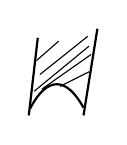
\begin{tikzpicture}[x=.88cm,y=.88cm,baseline]
\draw[thick] (0,0)--(.13,1.12) (.79,0)--(.99,1.25);
\draw[thick] (.02,.10) .. controls (.27,.58) and (.55,.55) .. (.79,.11);
\draw (.11,.79)--(.43,1.07);
\draw (.16,.59)--(.85,1.14);
\draw (.08,.35)--(.87,1.00);
\draw (.19,.38)--(.90,.88);
\draw (.45,.42)--(.87,.63);
\end{tikzpicture}}\endgroup}
\end{GelfandAdjacentEvidence}
\begin{GelfandAdjacentEvidence}{GELFAND-P000710}{3}


\underline{Теорема}: при нек-рых доп. усл. верно обратное, т. е.,
всякая решётка \uwave{арифметична}.
\uwave{Док-во} имеется в приложении к книге \uwave{Рагунатана}.

Для \(SL(2,\mathbb R)\) \uwave{неверно} --- есть параметры замощения плоскости Лобачевского, а арифм. подгрупп --- счётное число.

\underline{Гипотеза Сельберга}: для остальных групп она верна
Зигель тоже занимался.

\[
G=\prod G_i,\qquad G_i\text{ --- простые группы Ли}
\]
\uwave{Реш.} \(\Gamma\) наз. \uwave{приводимой}, если
\(G=G_1\times G_2\), \(\dim G_i>0\),
и \((G_1\cap\Gamma)\times(G_2\cap\Gamma)\) имеет конечный индекс в \(\Gamma\).

Изучаются \uwave{неприводимые решётки}.

\uwave{Гипотеза}: для неприв. подгруппы в \(G\ne SL(2,\mathbb R)/\{\pm E\}\)
[зачёркнуто: это?] \(\forall\) решётка арифметична.
\Unclear{GELFAND-P000710}{cancelled-before-universal}{Зачёркнутое слово перед \(\forall\) предположительно читается «это».}
\end{GelfandAdjacentEvidence}
\begin{GelfandAdjacentEvidence}{GELFAND-P000710}{4}


\uwave{Макаров, Винберг}: обнаружили неарифм. подгр. в группах движ. пр-в Лобачевского
\(SO(3,1)\), \(SO(4,1)\), \(SO(5,1)\)).

\underline{Ответ}: если
\[
\underline{\underline{\operatorname{rank}G\ge 2}},\quad\text{то теорема верна.}
\]
Параметр есть только в \(SL(2,\mathbb R)\).
В ост. случаях \uwave{жёсткость}. (Сельберг, А. Вейль)

\uwave{В ост. группах ранга 1 неизвестно}.

\uwave{Следствие теор. жёсткости} (Сельберг): \(\forall\) решётка
[зачёркнуто] в \(SL(n,\) [зачёркнуто] \(\mathbb R)\) сопряжена решётке с алгебраическими коэффициентами.
\Incomplete{GELFAND-P000710}{cancelled-after-lattice}{После «решётка» густо зачёркнута короткая запись.}
\end{GelfandAdjacentEvidence}
\begin{GelfandAdjacentEvidence}{GELFAND-P000710}{5}

\Incomplete{GELFAND-P000710}{cancelled-before-real-field}{В \(SL(n,\mathbb R)\) перед \(\mathbb R\) зачёркнут отдельный знак.}
\end{GelfandAdjacentEvidence}



\Needspace{7\baselineskip}
\begin{GelfandAdjacentEvidence}{GELFAND-P000711}{1}
\SourcePage{GELFAND-P000711}{44}
\underline{Основная лемма}.

Пусть \(G\) --- полупростая группа Ли,
[над строкой в обводке вставлено: \(\operatorname{rank}G\ge 2\)],
\(\Gamma\) --- [над строкой в обводке вставлено: неприводимая] решётка в \(G\),
[между строками вставлено: \(G\) не имеет компактных факторов],
\(k\) --- локальное поле хар-ки \(0\), т. е. \(\mathbb C\), \(\mathbb R\) или конечное расширение поля
\(\mathbb Q_p\), \(n\in\mathbb N\) и дан гомоморфизм
\(T:\Gamma\longrightarrow GL(n,k)\). Пусть

1) \(\overline{T(\Gamma)}\) связна и проста.
(замыкание по Зарисскому)

2) \(T(\Gamma)\) не является отн. компактной

Тогда

I. \(k=\mathbb C\) или \(\mathbb R\)
\(\Rightarrow\) \(T\) продолж. до предст. группы \(G\)

II. \(k=\mathbb Q_p\) \(\Rightarrow\) условия 1) и 2) противоречивы

\underline{Вывод теоремы из леммы}.

\(G=G(\mathbb R)\), \(K\) --- поле алг. чисел,
можно считать \(\Gamma\subset G(K)\)
(легко [над строкой вставлено: по теор. Сельберга] доказывается).

Пусть
\(\gamma_1,\ldots,\gamma_i\) --- образующие.
\Unclear{GELFAND-P000711}{last-generator-subscript}{Последний индекс предположительно \(i\); возможно \(l\).}
\end{GelfandAdjacentEvidence}
\begin{GelfandAdjacentEvidence}{GELFAND-P000711}{2}

Рассм. знаменатели соотв. матриц и вх. в их разложение простые множители \(p_1,\ldots,p_m\).
\Unclear{GELFAND-P000711}{last-prime-subscript}{Последний индекс в списке простых множителей исправлен; предположительно \(m\).}
\end{GelfandAdjacentEvidence}
\begin{GelfandAdjacentEvidence}{GELFAND-P000711}{3}


Дост. док., что образ
\Incomplete{GELFAND-P000711}{cancelled-before-gamma}{Перед \(\Gamma\) зачёркнута короткая запись.}
\end{GelfandAdjacentEvidence}
\begin{GelfandAdjacentEvidence}{GELFAND-P000711}{4}

\(\Gamma\) в \(G(\mathbb Q_p)\) относит. компактен.
Тогда знаменатели ограничены
\Incomplete{GELFAND-P000711}{cancelled-before-in-aggregate}{После «ограничены» зачёркнуто слово.}
\end{GelfandAdjacentEvidence}

в совок. (из устр. топологии в \(\mathbb Q_p\)).

Компактность следует из утв. II леммы. \(\blacksquare\)


\Needspace{7\baselineskip}
\begin{GelfandAdjacentEvidence}{GELFAND-P000712}{1}
\SourcePage{GELFAND-P000712}{unlabelled}
\underline{19/\(\overline{\underline{\mathrm{IX}}}\)---77 г.}
\quad \uwave{Сем. Гельфанда.}

\uwave{В. Дринфельд.} Рассм. \(S^4\) с конформной структурой, индуцированной стандартной метрикой.

\(\xi\) --- гладкое комплексное векторное расслоение над \(S^4\).

\Unclear{GELFAND-P000712}{preceding-physics-cancellation}{Зачёркнутая запись перед скобкой предположительно читается «Кир».}
\end{GelfandAdjacentEvidence}
\begin{GelfandAdjacentEvidence}{GELFAND-P000712}{2}

[Присутствует физик: Киржниц Давид Абрамович].

\uwave{Уравнения дуальности.} \quad \(A_\mu\) --- матричная ф-я 4-х перем.,
\begin{equation*}
F_{\mu\nu}=\partial_\mu A_\nu-\partial_\nu A_\mu+[A_\mu,A_\nu],
\qquad \mu=1,2,3,4.\tag{1}
\end{equation*}
\Unclear{GELFAND-P000712}{cancelled-before-duality}{Перед уравнением (2) зачёркнута запись, предположительно \(F_{ijk}\).}
\end{GelfandAdjacentEvidence}

\begin{equation*}
F_{ij}=\frac{1}{2}\varepsilon_{ijk\ell}F_{k\ell}
\qquad (\text{ур-я}\,\text{\uwave{дуальности}})\tag{2}
\end{equation*}
\begin{equation*}
[\partial_\mu+A_\mu,F_{\mu\nu}]=0
\qquad (\text{ур-я}\,\text{\uwave{Янга-Миллса}})\tag{3}
\end{equation*}


\Needspace{7\baselineskip}
\begin{GelfandAdjacentEvidence}{GELFAND-P000713}{1}
\SourcePage{GELFAND-P000713}{unlabelled}
\underline{Киржниц} \uwave{Давид Абрамович} (из ФИАН’а).

\uwave{О нек-рых характерных идеях теор. физики.}

\Unclear{GELFAND-P000713}{front-mark}{Перед «Передний край» отдельный знак, предположительно «4».}
\end{GelfandAdjacentEvidence}
\begin{GelfandAdjacentEvidence}{GELFAND-P000713}{2}

Передний край: 1) элем. частицы 2) космология 3) переход дин. систем в статист.

Всё это теперь тесно связано!

\Incomplete{GELFAND-P000713}{theory-mark}{Перед заголовком сильно переписанный или зачёркнутый знак.}
\end{GelfandAdjacentEvidence}
\begin{GelfandAdjacentEvidence}{GELFAND-P000713}{3}

\uwave{Теория элементарных частиц.}

Возн. \(\approx 50\) лет назад.

Первые 20 лет господств. идеи КТП, т. е. как в квант. механике.

\uwave{Конец 50-х годов}: сомнения.

\uwave{Ландау}: „Гамильт. метод --- труп. Наша зад. --- похоронить его со всеми причит. ему почестями!“

60-е годы --- групп. подход.

Теперь \uwave{ренессанс} полевого подхода. Виновата идея:

1. \uwave{Спонтанно нарушенная симметрия.}

Чувствит. к макроскоп. возд. (наруш. симметрии).

2. \uwave{Макроскопические воздействия.}

3. \uwave{История вселенной} --- пример
\(\overbrace{\text{наруш.}}^{\text{такого влияния}}\)
спонт. симм..

\uwave{Космология}

Вселенная горячая. Почему?

4. «Динамика --- статистика».

\uwave{Сначала о п. 4.} Неск. лет назад сказано принципиально новое слово:
\uwave{Hawking, Bekenstein}

обл. в фаз. пр-ве расползается (за счёт неустойчивости)
\SourceFigure{GELFAND-P000713}{phase-diagram}{%
\par\begingroup\color{black}\GelfandFitDiagram{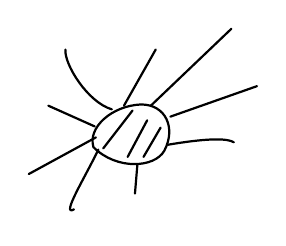
\begin{tikzpicture}[x=1.55cm,y=1.55cm,baseline,line cap=round]
\draw[thick] (-.32,-.12)
  .. controls (-.37,.04) and (-.17,.22) .. (.07,.23)
  .. controls (.27,.23) and (.36,.04) .. (.26,-.15)
  .. controls (.18,-.29) and (-.13,-.31) .. (-.32,-.12) -- cycle;
\draw[thick] (-.30,-.04)--(-.85,-.34)
  (-.28,-.14) .. controls (-.39,-.37) and (-.59,-.69) .. (-.48,-.63)
  (.04,-.26)--(.02,-.50)
  (.29,-.10) .. controls (.47,-.07) and (.75,-.03) .. (.83,-.08)
  (.31,.13)--(1.02,.38)
  (.15,.22)--(.81,.85)
  (-.07,.22)--(.19,.68)
  (-.17,.19) .. controls (-.37,.25) and (-.56,.56) .. (-.55,.68)
  (-.31,.05)--(-.69,.22);
\draw[thick] (-.24,-.13)--(.00,.18)
  (-.04,-.20)--(.12,.10)
  (.09,-.20)--(.23,.04);
\end{tikzpicture}}\endgroup}
\end{GelfandAdjacentEvidence}

--- было известно. (напр. биллиард Синая)

сист. с положит. энтропией.

\uwave{Информац. язык} (Сциллард, 1927 г, затем математики) здесь сработал.

Расползлось --- потеряли информацию
\[
\Delta I=\underline{\text{Информация}}=-\ln
\frac{P_f\;(\mathord{=}\text{число возм. ответа на вопр. в конце})}
{P_i\;(\mathord{=}\text{--- ″ --- в начале})}
\]

\uwave{Энтропия}

Макросост. опр. малым числом \uwave{параметров}. При них возможны различные распр. частиц (вырождение).

Энтропия \(S=\ln(N_{\text{микроскоп}})\)

\underline{И. М. Г.}: Энтропия: 27 монет, 1 фальш. легче др. --- 3 взвеш.

\(N\) монет, 1 фальш. отл. по весу, при каком \(N\) можно найти за 3 взвешивания:

\underline{Решение}: \uwave{вдвое меньше знаем} (\underline{\underline{13}}).

\(N\) взвеш. \((3^N-1)/2\).


\Needspace{7\baselineskip}
\begin{GelfandAdjacentEvidence}{GELFAND-P000714}{1}
\SourcePage{GELFAND-P000714}{47}
\underline{Алгоритм.}

Делить монеты надо. так, чтобы энтропия кучек была одинакова!!

(Дел. энтроп. на 3 одинаков. части).

Не надо перебора!

\begin{tabular}{@{}ll@{}}
монета & \(p\) --- вер. орла \\
       & \(q\) --- вер. решки
\end{tabular}
\[
S=p\ln p+q\ln q
\]
\Unclear{GELFAND-P000714}{binary-entropy-sign}{Перед \(p\ln p\) в рукописи минус не виден.}
\end{GelfandAdjacentEvidence}
\begin{GelfandAdjacentEvidence}{GELFAND-P000714}{2}


Из аддит. получ. разумность.

\uwave{\(N\) исх.} \quad \(-\sum p_i\ln p_i\)
\qquad Если \(p_i=\frac{1}{N}\), то получ. \(S=\ln N\)

\uwave{Информ.} \(=\) \uwave{изменение энтропии.}

\uwave{Реш. зад.}: смотреть измен. вероятностей.

Начало: \underline{\(4+4,5\)}
\[
\Delta I=-\ln\frac{N_f}{N_i}
\]

\uwave{К. Д. А.}\quad \uwave{\(\Delta S=-\Delta I.\)}

\underline{Пример}: газ
\SourceFigure{GELFAND-P000714}{gas-states}{%
\par\begingroup\color{black}\GelfandFitDiagram{\begin{tikzpicture}[x=.85cm,y=.85cm,baseline]
\draw (0,0) rectangle (1.45,.68);
\draw (.73,0)--(.73,.68);
\draw (.01,.34)--(.46,.62) (.13,.21)--(.60,.56)
  (.15,.12)--(.59,.40) (.14,.03)--(.63,.28);
\node[below] at (.725,0) {нач. сост.};
\draw (2.38,0) rectangle (3.83,.68);
\draw (2.38,.36)--(2.75,.68) (2.60,.20)--(3.12,.64)
  (2.82,.12)--(3.41,.65) (3.09,.05)--(3.65,.57)
  (3.47,.04)--(3.83,.37);
\node[below] at (3.105,0) {конечное};
\end{tikzpicture}}\endgroup}
\end{GelfandAdjacentEvidence}
\begin{GelfandAdjacentEvidence}{GELFAND-P000714}{3}

\[
S=\ln\frac{V}{N}\qquad(\text{на одну молекулу}).
\]
\begin{center}
\begingroup\color{black}\GelfandFitDiagram{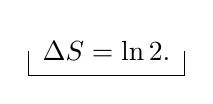
\begin{tikzpicture}
\node (delta) [inner sep=5pt] {\(\Delta S=\ln 2.\)};
\draw (delta.west)--(delta.south west)--(delta.south east)--(delta.east);
\end{tikzpicture}}\endgroup
\end{center}

Следствие: потеря инф. \(\Rightarrow\) рост энтропии

Приобрели инф. \(\Rightarrow\) уменьш. инф.
\Unclear{GELFAND-P000714}{acquisition-consequence}{Начало «уменьш.» переписано, а следующее сокращение читается «инф.».}
\end{GelfandAdjacentEvidence}
\begin{GelfandAdjacentEvidence}{GELFAND-P000714}{4}


Демон Максв. пониж. энтропию (следит за частицами)

Есть ли ещё способы потери инф.?

Может быть, есть
\Incomplete{GELFAND-P000714}{forces-cancellation}{После «есть» густо зачёркнуто слово.}
\end{GelfandAdjacentEvidence}
\begin{GelfandAdjacentEvidence}{GELFAND-P000714}{5}

силы, удерж. информацию
\Incomplete{GELFAND-P000714}{before-volume-cancellation}{Перед «в д. объёме» зачёркнут отдельный знак.}
\end{GelfandAdjacentEvidence}

в д. объёме.

\uwave{Изв. ситуация, когда информ. отсекается физич. средствами}

--- не выходит инф.

Есть такая сила: \underline{тяготение}! (и она единственная)

Дальнодейств. и одного знака (!)

«Чёрная дыра» --- тело, не выпускающ. информацию.

Придумал Лаплас: \uwave{Скор. света \(=2^{\underline{\text{й}}}\) космич. скор.}
\[
\frac{mv^2}{2}-\gamma\frac{mM}{R}=0
\]
\[
\frac{mc^2}{2}=\gamma\frac{mM}{R},
\]
\[
\boxed{R=\frac{2\gamma M}{c^2}=r_g}
\]

При таком радиусе свет не покинет тело (и никакой сигнал)

--- оказывается, верно и в точной науке


\Needspace{7\baselineskip}
\begin{GelfandAdjacentEvidence}{GELFAND-P000715}{1}
\SourcePage{GELFAND-P000715}{unlabelled}
\[
R_{\text{солнца}}=10^6\ \text{км}
\]
\Unclear{GELFAND-P000715}{mass-cancellation}{Перед «Для» густо зачёркнут один знак.}
\end{GelfandAdjacentEvidence}
\begin{GelfandAdjacentEvidence}{GELFAND-P000715}{2}

Для его массы нужен рад. \underline{\underline{\(7\) км.}}

О чёрной дыре принцип. ничего не можем знать, кроме неск. пар. ---
--- массы, заряда,
\Incomplete{GELFAND-P000715}{charge-cancellation}{Запись после «заряда» густо зачёркнута.}
\end{GelfandAdjacentEvidence}
\begin{GelfandAdjacentEvidence}{GELFAND-P000715}{3}

радиуса.

Как в случае газа. Микросост. огромное количество.
На самом деле это \uwave{термодин. объект}!!

\(\underset{\text{(раньше)}}{\text{\uwave{Хокинг}}}\):
пов. чёрной дыры \(S\) (!) возрастает при всех процессах.
Слияние 2-х чёрных дыр. Геом. ясно увелич. (из ф-мы Лапласа)

Буква \(S\) сыграла замеч. роль.
\[
\begingroup\color{black}\GelfandFitDiagram{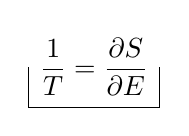
\begin{tikzpicture}[baseline=(definition.base)]
\node (definition) [inner sep=4pt] {\(\displaystyle \frac{1}{T}=\frac{\partial S}{\partial E}\)};
\draw (definition.west)--(definition.south west)--(definition.south east)--(definition.east);
\end{tikzpicture}}\endgroup
\quad\Rightarrow\quad T\text{ --- „темпер.“ чёрной дыры.}
\]

\(\underset{\text{(уч. Хокинга)}}{\text{\uwave{Bekenstein}}}\) ---
снял кавычки! Посчитал информацию, теряющуюся при постр. чёрных дыр!!
Совп. с энтр. информационной.

Кинем горячее тело на чёрную дыру. Оно увелич. пов. больше, чем холодное, в точн. соотв. возраст. энтропии.

[зачёркнуто: Хокинг.] \underline{\underline{Хокинг}}.
Слияние пар частиц. Чёрная дыра излучает и спектр планковский!
\[
\frac{1}{e^{\frac{\hbar\omega}{kT}}-1}
\]
\(T\) --- та температура.

Информ. тер. не стохастизацией!!, а уходит в чёрные дыры.
(механич. отсекается)

Другие способы

\uwave{\href{https://doi.org/10.1103/PhysRevD.14.870}{Uhnru?}}
\Unclear{GELFAND-P000715}{unruh-name}{Написание фамилии предположительно «Uhnru». По смыслу речь об \href{https://doi.org/10.1103/PhysRevD.14.870}{У. Г. Унру}.}
\end{GelfandAdjacentEvidence}
\begin{GelfandAdjacentEvidence}{GELFAND-P000715}{4}

Однор. поле тяготения.

Пусть в вакууме част. двиг. равномерно ускоренно.
До неё дойдёт свет не отовсюду.

\SourceFigure{GELFAND-P000715}{unruh-diagram}{%
\par\begingroup\color{black}\GelfandFitDiagram{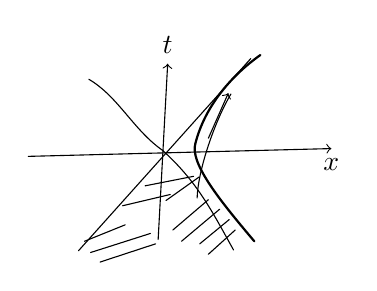
\begin{tikzpicture}[x=1.1cm,y=1.1cm,baseline,line cap=round]
\draw[->] (-1.55,-.07)--(1.95,.02) node[below] {\(x\)};
\draw[->] (-.05,-1.03)--(.06,1.0) node[above] {\(t\)};
\draw (-.97,-1.16)--(1.02,1.06);
\draw (-.85,.82) .. controls (-.51,.62) and (-.34,.24) .. (0,0)
  .. controls (.40,-.36) and (.57,-.70) .. (.82,-1.15);
\draw[thick] (1.06,-1.05) .. controls (.68,-.60) and (.31,-.15) .. (.38,.08)
  .. controls (.48,.47) and (.75,.83) .. (1.13,1.10);
\draw (.40,-.55) .. controls (.41,-.23) and (.60,.33) .. (.79,.65);
\draw[->] (.53,.14)--(.76,.66);
\draw (-.83,-1.18)--(-.14,-.96) (-.72,-1.29)--(-.08,-1.08)
  (-.90,-1.05)--(-.43,-.86) (-.46,-.64)--(.09,-.51)
  (-.20,-.41)--(.36,-.30) (.04,-.58)--(.42,-.31)
  (.12,-.92)--(.53,-.57) (.22,-1.05)--(.66,-.68)
  (.43,-1.08)--(.77,-.80) (.53,-1.20)--(.84,-.92);
\end{tikzpicture}}\endgroup\par\smallskip
В местах наложения правых кривых и штрихов их точное соединение неразличимо.}
\end{GelfandAdjacentEvidence}
\begin{GelfandAdjacentEvidence}{GELFAND-P000715}{5}


Получ., что свет дох. лишь от \uwave{половины пр-ва}.
Наблюд. увидит (расчёт) \uwave{планковское распред.}.
Нулевые колеб. он видит перекошенными.
Это тяжёлый счёт.

\(H\) --- гам. эл.-магн. поля.
\[
H\lvert\Phi\rangle=E_0\lvert\varphi\rangle
\]
\Unclear{GELFAND-P000715}{hamiltonian-state}{Знак состояния слева сильно обведён и выглядит как \(\Phi\); справа знак выглядит как \(\varphi\).}
\end{GelfandAdjacentEvidence}
\begin{GelfandAdjacentEvidence}{GELFAND-P000715}{6}


Вектор сост. с точки зр. неинерц. наблюд. \(\rightarrow\) Счит. вер.
\(1^{\underline{\text{го}}}\), \(2^{\underline{\text{х}}}\) и более

\Unclear{GELFAND-P000715}{outer-right-fragments}{За правой границей страницы видны два обрезанных фрагмента штрихов.}
\end{GelfandAdjacentEvidence}



\Needspace{7\baselineskip}
\begin{GelfandAdjacentEvidence}{GELFAND-P000716}{1}
\SourcePage{GELFAND-P000716}{48?}
\Unclear{GELFAND-P000716}{folio}{Последняя цифра номера предположительно 8, возможно 2.}
\end{GelfandAdjacentEvidence}
\begin{GelfandAdjacentEvidence}{GELFAND-P000716}{2}

фотонов.
\[
\begingroup\color{black}\GelfandFitDiagram{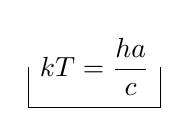
\begin{tikzpicture}[baseline=(temp.base)]
\node (temp) [inner sep=4pt] {\(\displaystyle kT=\frac{ha}{c}\)};
\draw (temp.west)--(temp.south west)--(temp.south east)--(temp.east);
\end{tikzpicture}}\endgroup\quad\Rightarrow\quad\text{температура}
\]
\Unclear{GELFAND-P000716}{temperature-constant}{Первый знак числителя читается \(h\); отдельная черта для \(\hbar\) неразличима.}
\end{GelfandAdjacentEvidence}
\begin{GelfandAdjacentEvidence}{GELFAND-P000716}{3}


Нагрев. газа на финише.

\uwave{Почему вселенная горячая?}

[Слева] Эксперимент --- остывает сейчас \(\Vert\)

[Справа] \underline{\underline{\(T=3^{\circ}\mathrm K\)}} --- из распр.
\Incomplete{GELFAND-P000716}{temperature-cancellation}{Перед «Планка» густо зачёркнуто слово.}
\end{GelfandAdjacentEvidence}
\begin{GelfandAdjacentEvidence}{GELFAND-P000716}{4}

Планка излуч. из космоса.
[под формулой: (реликтовое излучение)]

Область неизвестности была.
Возникла в какой-то момент времени. До этого бессмысленно [ниже: спрашивать].

\uwave{Есть горизонт событий}.
\SourceFigure{GELFAND-P000716}{horizon-drawing}{%
\par\begingroup\color{black}\GelfandFitDiagram{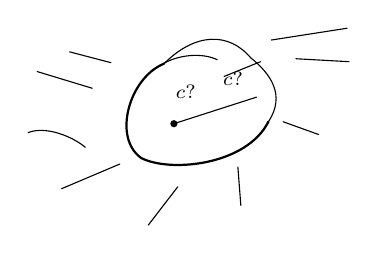
\begin{tikzpicture}[x=1.25cm,y=1.25cm,baseline,line cap=round]
\draw[thick] (-.30,.46) .. controls (-.65,.32) and (-.83,-.29) .. (-.53,-.50)
  .. controls (-.23,-.65) and (.54,-.57) .. (.76,-.13);
\draw (.76,-.13) .. controls (.94,.14) and (.78,.36) .. (.58,.52)
  .. controls (.36,.78) and (.02,.78) .. (-.30,.46);
\draw (-.31,.46) .. controls (-.11,.57) and (.12,.56) .. (.24,.50);
\draw (-1.26,.58)--(-.84,.47) (-1.59,.38)--(-1.03,.21)
  (-1.68,-.24) .. controls (-1.50,-.17) and (-1.23,-.28) .. (-1.10,-.39)
  (-1.34,-.81)--(-.75,-.56) (-.46,-1.18)--(-.16,-.79)
  (.48,-.98)--(.45,-.59) (.79,.70)--(1.56,.82)
  (1.04,.51)--(1.58,.48) (.91,-.13)--(1.27,-.26);
\fill (-.20,-.15) circle[radius=1.3pt];
\draw (-.20,-.15)--(.64,.12) (.31,.33)--(.68,.48);
\node at (-.08,.17) {\scriptsize\(c?\)};
\node at (.40,.31) {\scriptsize\(c?\)};
\end{tikzpicture}}\endgroup\par\smallskip
Концы внутренних линий и два малых знака различимы частично.}
\end{GelfandAdjacentEvidence}
\begin{GelfandAdjacentEvidence}{GELFAND-P000716}{5}

\underline{закрытая обл.} (свет не успел дойти оттуда).
(\(\Rightarrow\) поэтому для нас такая темпер.)

\begin{center}
\rule[.45ex]{1.4em}{.35pt}\,\(\cdot\)\,\rule[.45ex]{1.4em}{.35pt}
\end{center}
Спонтанное наруш. симм.
\SourceFigure{GELFAND-P000716}{symmetry-curves}{%
\par\begingroup\color{black}\GelfandFitDiagram{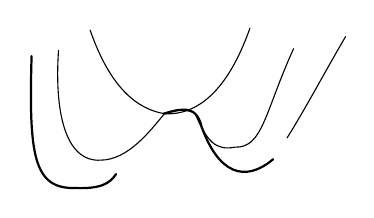
\begin{tikzpicture}[x=1.18cm,y=1.18cm,baseline,line cap=round]
\draw (-.84,.90) .. controls (-.62,.27) and (-.33,.05) .. (-.04,0)
  .. controls (.31,-.02) and (.64,.24) .. (.88,.92);
\draw (-1.18,.68) .. controls (-1.23,-.07) and (-1.07,-.52) .. (-.73,-.50)
  .. controls (-.43,-.50) and (-.19,-.18) .. (-.04,0)
  .. controls (.04,.05) and (.22,.06) .. (.29,.00)
  .. controls (.42,-.30) and (.51,-.40) .. (.72,-.36)
  .. controls (1.02,-.37) and (1.04,.02) .. (1.35,.70);
\draw[thick] (-1.47,.62) .. controls (-1.50,-.45) and (-1.45,-.81) .. (-1.00,-.80)
  .. controls (-.72,-.81) and (-.63,-.75) .. (-.56,-.65);
\draw[thick] (-.05,0) .. controls (.11,.04) and (.30,.12) .. (.36,-.14)
  .. controls (.54,-.64) and (.82,-.75) .. (1.13,-.49);
\draw (1.28,-.26) .. controls (1.47,.04) and (1.72,.51) .. (1.91,.83);
\end{tikzpicture}}\endgroup\par\smallskip
Точные продолжения линий в месте наложения неразличимы.}
\end{GelfandAdjacentEvidence}
\begin{GelfandAdjacentEvidence}{GELFAND-P000716}{6}

\uwave{эволюция ямы при наруш. температуры}
\Unclear{GELFAND-P000716}{minimum-temperature}{Подпись предположительно читается «эволюция ямы при наруш. температуры»; возможное чтение «мин» вместо «ямы».}
\end{GelfandAdjacentEvidence}


\begin{center}
\rule[.45ex]{2.1em}{.45pt}\,\(\cdot\)\,\rule[.45ex]{2.1em}{.45pt}
\end{center}
Идея \uwave{Сени Вишика}, о том, почему сем. Гельфанда нестерилизован:
„Чтобы успешно проинтегрировать большую область, надо пользоваться методом Монте-Карло“.


\Needspace{7\baselineskip}
\begin{GelfandAdjacentEvidence}{GELFAND-P000717}{1}
\SourcePage{GELFAND-P000717}{55}
\underline{3/\(\overline{\underline{\mathrm X}}\)---77 г.}
\qquad \underline{Сем. Гельфанда.}

\begin{flushright}
Будет систематически: «некоммутативная алгебраическая геометрия»
\end{flushright}

\underline{\underline{Л. А. Дикий.}}\qquad \underline{О новых алгебрах Ли.}

(\uwave{Гельф., Дикий}, \href{https://www.mathnet.ru/eng/faa2064}{Функ. анализ, 11:2}).

Def. 1. \quad \uwave{Алгебра \(A\).}

\Unclear{GELFAND-P000717}{cancelled-top}{Справа зачёркнуто «В» и ещё одно слово, предположительно «себе».}
\end{GelfandAdjacentEvidence}
\par\begingroup\setlength{\parindent}{0pt}\setlength{\parskip}{.4em}\raggedright


\[
u_k^{(i)},\qquad k=0,1,\ldots,n;\qquad i=0,1,2,\ldots
\]
\[
A=\left\{\sum a\,u_{k_1}^{(i_1)}u_{k_2}^{(i_2)}u_{k_3}^{(i_3)}
\cdots u_{k_N}^{(i_N)}\right\},\qquad a\in\underset{\text{(поле)}}{K},
\]
\begin{flushright}
\(A\) --- алг. многочленов\\
от образующих \(u_k^{(i)}\)\\
\fbox{\(A=K[u_k^{(i)}].\)}
\end{flushright}
\[
\xi=\sum a_{k,i}\frac{\partial}{\partial u_k^{(i)}},\qquad a_{k,i}\in A.
\]
(сумма бесконечна)\qquad \(\xi\) наз. дифференцированием
\[
\frac{d}{dx}=\sum_{k,i}u_k^{(i+1)}\frac{\partial}{\partial u_k^{(i)}}
\]
\[
\frac{d}{dx}u_k^{(i)}=u_k^{(i+1)};\qquad
u_k^{(i)}=\left(\frac{d}{dx}\right)^i u_k;\qquad
u_k\underset{\mathrm{def}}{=}u_k^{(0)}
\]

\underline{Def.} 2. \quad \uwave{Пространство} \(\widetilde A\) (пр-во функционалов)

В дальнейшем всегда \(u_n=1\), \(u_{n-1}=0\).
\[
\left\{f:\ \exists g,\ f=\frac{d}{dx}g\right\}=\frac{d}{dx}A;
\]
\[
\widetilde A=A\big/\frac{d}{dx}A
\]
\[
f\longmapsto f\bmod\frac{d}{dx}A=\widetilde f\in\widetilde A
\]
\[
A\underset{\int\cdots\,dx}{\longrightarrow}\widetilde A
\qquad\qquad
\widetilde f=\int f\,dx
\]

\underline{Задача.}
\[
f[u]\in\mathbb C[u_k^{(i)}];
\]
\[
\int_{-\infty}^{\infty}f[u(x)]\,dx=0,\quad\forall u\in S(\mathbb R^1)
\quad\Longleftrightarrow\quad
f\in\frac{d}{dx}\mathbb C[u].
\]

\par\endgroup
\begin{GelfandAdjacentEvidence}{GELFAND-P000717}{2}
\underline{Def. 3}. \quad
\(A^{n-1}={}\) пр-во наборов \((f_0,f_1,\ldots,f_{n-2})\), \(f_k\in A\)

[на левом поле: \(\frac{\delta}{\delta u}\).]
\[
\frac{\delta}{\delta u}:\widetilde A\longrightarrow A^{n-1}
\]
\[
\left(\frac{\delta\widetilde f}{\delta u}\right)_k
=\sum_{\ell=0}^{\infty}\left(-\frac{d}{dx}\right)^\ell
\frac{\partial f}{\partial u_k^{(\ell)}}
=\frac{\delta\widetilde f}{\delta u_k}
\]
\Unclear{GELFAND-P000717}{variational-numerator}{В числителе под суммой \(f\) обведено более толстыми штрихами.}
\end{GelfandAdjacentEvidence}

(здесь \(\widetilde f=f\bmod\frac{d}{dx}A\))


\Needspace{7\baselineskip}
\begin{GelfandAdjacentEvidence}{GELFAND-P000718}{1}
\SourcePage{GELFAND-P000718}{unlabelled}
\underline{Def. 4.}\quad \(\ell:A^{n-1}\longrightarrow A^{n-1}\)
\[
f=(f_0,\ldots,f_{n-2})
\]
\[
(\ell f)_r=\sum_s\ell_{rs}f_s
\]
\[
\begin{aligned}
\ell_{rs}&=\sum_{\gamma=0}^{n-1-r-s}
\Biggl[\binom{\gamma+r}{r}u_{r+s+\gamma+1}
\left(-i\frac{d}{dx}\right)^\gamma-\\
&\qquad-\binom{\gamma+s}{s}\left(i\frac{d}{dx}\right)^\gamma
u_{r+s+\gamma+1}\Biggr]
\end{aligned}
\]
\Unclear{GELFAND-P000718}{operator-line-break}{В рукописи минус повторён при переносе: в конце первой строки и в начале второй.}
\end{GelfandAdjacentEvidence}
\par\begingroup\setlength{\parindent}{0pt}\setlength{\parskip}{.4em}\raggedright


\underline{\(n=2,3\)} просто;\qquad \underline{\(n=4\)} --- 1-й содерж. пример.

\underline{Def. 5.}\quad \(\forall f\in A^{n-1}\) построим
\[
\partial_f=\sum_{k,\ell}f_k^{(\ell)}\frac{\partial}{\partial u_k^{(\ell)}}
\qquad\text{(дифференцирование)}
\]
Легко проверить, что
\[
\partial_f\frac{d}{dx}=\frac{d}{dx}\partial_f
\]
Поэтому определена операция \(\partial_f:\widetilde A\longrightarrow\widetilde A\).

\underline{Def. 6.}\quad Пусть \(f,g\in A^{n-1}\). Положим
\[
([f,g])_r=\partial_f g_r-\partial_g f_r
\]
Легко проверить, что
\[
[\partial_f,\partial_g]=\partial_{[f,g]}.
\]
Поэтому коммутатор \([\cdot,\cdot]\) определяет на \(A^{n-1}\) структуру алгебры Ли.

\underline{Def. 7.}\quad опр. коммутатор в \(\widetilde A\).
\[
\{\widetilde f,\widetilde g\}
=\int\sum_{r,s}\frac{\delta\widetilde f}{\delta u_r}\cdot
\ell_{rs}\frac{\delta\widetilde g}{\delta u_s}\,dx
\]

\par\endgroup
\begin{GelfandAdjacentEvidence}{GELFAND-P000718}{2}
\underline{Теорема:}
\Incomplete{GELFAND-P000718}{theorem-cancellation}{После «Теорема» густо зачёркнуто слово.}
\end{GelfandAdjacentEvidence}
\begin{GelfandAdjacentEvidence}{GELFAND-P000718}{3}

получается алгебра Ли
\Unclear{GELFAND-P000718}{theorem-verb}{Глагол предположительно «получается», возможно «получится».}
\end{GelfandAdjacentEvidence}

(т. е. выполнено тождество Якоби)

\underline{Задача:} доказать её попроще.

\underline{С. П. Новиков}\qquad
\(A=\frac{d^3}{dx^3}+\left(u\frac{d}{dx}+\frac{d}{dx}u\right)\)

тоже задаёт алгебру Ли.

(и с помощью него можно записать ур-е КдФ).


\Needspace{7\baselineskip}
\begin{GelfandAdjacentEvidence}{GELFAND-P000719}{1}
\SourcePage{GELFAND-P000719}{56}
\underline{С. И. Гельфанд.} о раб. И. М. Гельф., И. Н. Бернш. и свои.:
\Unclear{GELFAND-P000719}{heading-final-word}{Последнее слово заголовка предположительно читается «свои.»; конечные штрихи сливаются.}
\end{GelfandAdjacentEvidence}
\begin{GelfandAdjacentEvidence}{GELFAND-P000719}{2}


\begin{flushright}
\fbox{\parbox{.66\linewidth}{«Локальная структура категории модулей Хариш-Чандры»\\или «Некоммутативная алгебраическая геометрия I».}}
\end{flushright}

\(G\) --- вещественная группа Ли, полупростая

\(K\subset G\), \(K\) --- максимальная компактная подгруппа

\(\mathfrak g\) --- алгебра Ли группы \(G\)

\underline{Определение.} Модуль Хариш-Чандры \(M\) ---
это линейное пр-во над \(\mathbb C\) с действием \(\mathfrak g\) и \(K\) и с условиями
(кроме естеств. условий действия и согласования действий \(\mathfrak g\) и \(K\)).

1) действия [зачёркнуто: алгебры Ли группы \(K\)] \(\mathfrak g\) и \(K\) согласованы:

а) алг. Ли \(K\) действует на \(M\) как подалгебра в \(\mathfrak g\).

б) [зачёркнуто: а)?]
\Unclear{GELFAND-P000719}{canceled-condition-label}{После «б)» зачёркнут знак, предположительно «а)».}
\end{GelfandAdjacentEvidence}
\begin{GelfandAdjacentEvidence}{GELFAND-P000719}{3}

\[
T\bigl(\underset{\substack{\uparrow\\K}}{k}\,
\underset{\substack{\uparrow\\\mathfrak g}}{X}\,k^{-1}\bigr)
=T_1(k)T(X)T_1(k^{-1}).
\]
\(T\) --- действие \(\mathfrak g\), \(T_1\) --- действие \(K\)

2) \(M\) разбив. отн. \(K\) в прямую сумму [вставлено сверху: неприв.]
представлений и каждое [вставлено снизу: неприв.] предст. встречается конечное число раз.

М. Х.-Ч. обр. \uwave{категорию}. Морфизмы определяются естеств. образом.

\uwave{Задача}: описание этой категории.

\uwave{Идея}: есть некоммут. алгебра, к-рая за это ответственна.

\uwave{\href{https://www.mathnet.ru/eng/rm5609}{Гельфанд, Пономарев}}:
для группы Лоренца [вставлено снизу: \(SL(2,\mathbb C)\)] свод. к классификации таких пар матриц
\(A,B\), что \(AB=BA=0\),
[зачёркнуто: и]
\Incomplete{GELFAND-P000719}{canceled-matrices}{После «и» зачёркнуты ещё два слова.}
\end{GelfandAdjacentEvidence}
\begin{GelfandAdjacentEvidence}{GELFAND-P000719}{4}


\(U(\mathfrak g)\) --- обёртыв. алгебра \(\mathfrak g\)

\(Z(\mathfrak g)\) --- её центр

\[
M\rightsquigarrow J_M=\{z\in Z(\mathfrak g)\mid zM=0\}
\qquad\text{(идеал) в }Z(\mathfrak g).
\]

\(\Theta\) --- множество характеров \(\theta:Z(\mathfrak g)\to\mathbb C\).
(гомоморфизмов)

[зачёркнуто под формулой: (линейные ф-лы?)] \((\subset\mathbb C^N)\).
\Unclear{GELFAND-P000719}{canceled-theta-abbrev}{В зачёркнутой записи сокращение после «линейные» предположительно «ф-лы».}
\end{GelfandAdjacentEvidence}
\begin{GelfandAdjacentEvidence}{GELFAND-P000719}{5}

\Unclear{GELFAND-P000719}{theta-ambient-exponent}{В \(\mathbb C^N\) регистр показателя неясен: \(N\) или \(n\).}
\end{GelfandAdjacentEvidence}


\begin{gather*}
\operatorname{supp}M\subset\Theta\\
\operatorname{supp}M=\{\theta\mid J_M\subset\ker\theta\}
\end{gather*}
\(\operatorname{supp}M\) --- конечное мн-во.

Пусть \(D\subset\Theta\),
\[
C_D=\{M\mid\operatorname{supp}M\subset D\}.
\]


\Needspace{7\baselineskip}
\begin{GelfandAdjacentEvidence}{GELFAND-P000720}{1}
\SourcePage{GELFAND-P000720}{unlabelled}
Можно рассм. модули Х.-Ч. с носит. в точке \(C_{\{\theta\}}\)

\underline{Теорема} (лёгкая).
\[
C_D=\bigoplus_{\theta\in D}C_{\{\theta\}}
\]
\Incomplete{GELFAND-P000720}{canceled-sum-symbol}{Между знаком равенства и \(\bigoplus\) зачёркнут знак.}
\end{GelfandAdjacentEvidence}
\begin{GelfandAdjacentEvidence}{GELFAND-P000720}{2}

в нек-ром смысле,

(разлагаются и нет гомоморфизмов).

\underline{1-я основная теорема.} Пусть \(D\) --- огр. область в \(\Theta\)
(в компл. смысле). Тогда \(\exists\ Z(\mathfrak g)\)-алгебра \(Q\)
\Unclear{GELFAND-P000720}{algebra-canceled-sign}{Справа внизу от \(Q\) зачёркнут небольшой знак, возможно индекс.}
\end{GelfandAdjacentEvidence}
\begin{GelfandAdjacentEvidence}{GELFAND-P000720}{3}

[зачёркнуто: такая] с конечным числом \(a\) аддитивных \(Z(\mathfrak g)\)-образующих,
[вставлено сверху: такая что] [зачёркнуто: Тогда?]
\(C_D\) эквивалентна категории \(Q\)-модулей, которые конечномерны над \(\mathbb C\).
\Unclear{GELFAND-P000720}{canceled-theorem-word}{Зачёркнутое слово перед \(C_D\) предположительно «Тогда».}
\end{GelfandAdjacentEvidence}
\begin{GelfandAdjacentEvidence}{GELFAND-P000720}{4}


(\(\exists\) функтор, осущ. эквивалентность)

\(Q\) --- \(Z(\mathfrak g)\)

\begin{center}--- \(\cdot\) ---\end{center}

\(\underset{23/\overline{\underline{\mathrm{IX}}}\text{-}77}{\text{«Известия»}}\)
и
\(\underset{22/\overline{\underline{\mathrm{IX}}}\text{-}77}{\text{«Соц. индустрия»}}\)
[зачёркнуто: от 23]

сообщение из Петрозаводска о неопознанном летающем объекте

\begin{center}--- \(\cdot\) ---\end{center}

\underline{Пример.}
\begin{gather*}
G=SL_2(\mathbb R)/\{\pm1\}\\
Z(\mathfrak g)\cong\mathbb C[z]\\
\Theta=\mathbb C^1
\end{gather*}

\SourceFigure{GELFAND-P000720}{central-character-disk}{%
\par\begingroup\color{black}\GelfandFitDiagram{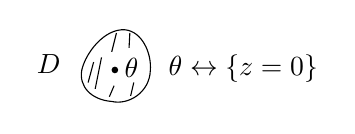
\begin{tikzpicture}[baseline]
\node at (-.87,.06) {\(D\)};
\draw (-.45,-.02) .. controls (-.40,.20) and (-.16,.51) .. (.10,.49)
  .. controls (.31,.47) and (.44,.20) .. (.42,-.03)
  .. controls (.41,-.30) and (.15,-.47) .. (-.07,-.42)
  .. controls (-.33,-.40) and (-.49,-.23) .. (-.45,-.02);
\draw (-.37,-.18)--(-.30,.08) (-.28,-.26)--(-.20,.14)
  (-.07,.21)--(-.01,.45) (.15,.26)--(.16,.45)
  (-.10,-.36)--(-.04,-.22) (.17,-.35)--(.21,-.18);
\fill (-.03,-.02) circle[radius=1.2pt];
\node at (.18,.00) {\(\theta\)};
\node at (1.60,.00) {\(\theta\leftrightarrow\{z=0\}\)};
\end{tikzpicture}}\endgroup}
\end{GelfandAdjacentEvidence}


Алгебру будем строить над аналит. ф-ями
\[
Q=(a_{ij}(z))_{i,j=1}^{3}\text{ --- матр. }3\times3,
\qquad a_{ij}(z)\text{ --- целые ф-и}
\]
\[
(a_{ij}(0))=
\begin{pmatrix}
*&0&0\\
*&*&0\\
*&0&*
\end{pmatrix}
\]


\Needspace{7\baselineskip}
\begin{GelfandAdjacentEvidence}{GELFAND-P000721}{1}
\SourcePage{GELFAND-P000721}{unlabelled}
\underline{10/\(\overline{\underline{\mathrm X}}\)---77 г.}
\qquad\underline{\underline{Сем. Гельфанда.}}

\underline{С. Гельфанд.}

\(G\) --- полупростая вещественная группа Ли

\(K\) --- максимальная компактная подгруппа

\(\mathfrak g\) --- алгебра Ли группы \(G\)

\(U(\mathfrak g)\) --- обёртывающая алгебра.

\(Z(\mathfrak g)\) --- центр \(U(\mathfrak g)\)

Модуль Хариш-Чандры (МХЧ) \(V\), если

[\underline{Теор. Х.-Ч.:} в непривод. предст. полупростой группы каждое
[вставлено сверху: неприв.] предст. макс. комп. группы \(K\) встреч. конечн. число раз]

В \(V\) заданы предст. \(T_1\) алг. \(U(\mathfrak g)\), \(T_2\) --- предст. группы \(K\).

1) \(V\) --- конечно порожд. \(U(\mathfrak g)\)-модуль.

2) \(\left.T_1\right|_{\mathfrak k}=dT_2\),
\[
T_2(k)T_1(X)T_2(k^{-1})=T_1(kXk^{-1})
\]

3) \(T_2=\bigoplus\) неприв. непр. предст. \(K\), причём каждое встречается конечное число раз.

(прямая сумма в букв. смысле).

\Incomplete{GELFAND-P000721}{canceled-result-heading}{Перед «Результат» густо зачёркнута короткая запись.}
\end{GelfandAdjacentEvidence}
\begin{GelfandAdjacentEvidence}{GELFAND-P000721}{2}

\underline{Результат:} пусть
\[
\Theta=\{\theta:Z(\mathfrak g)\to\mathbb C\}=\mathbb C^{r}
\]
\Unclear{GELFAND-P000721}{theta-exponent}{Показатель предположительно \(r\), возможно \(\tau\).}
\end{GelfandAdjacentEvidence}
\begin{GelfandAdjacentEvidence}{GELFAND-P000721}{3}

(кольцевые гомоморфизмы)

\[
V\mapsto\operatorname{supp}V\subset\Theta
\]
\[
\theta(z)\in\operatorname{supp}V
\Longleftrightarrow\exists\underset{\substack{\uparrow\\V}}{v}:
T_1(z)v=\theta(z)v,\quad z\in Z(\mathfrak g).
\]
\Unclear{GELFAND-P000721}{support-criterion}{Слева в рукописи стоит \(\theta(z)\), а условия \(v\ne0\) рядом нет.}
\end{GelfandAdjacentEvidence}
\begin{GelfandAdjacentEvidence}{GELFAND-P000721}{4}


На самом деле
\Incomplete{GELFAND-P000721}{canceled-support-symbol}{Под вставкой «\(\operatorname{supp}V\) —» густо зачёркнута короткая запись.}
\end{GelfandAdjacentEvidence}
\begin{GelfandAdjacentEvidence}{GELFAND-P000721}{5}

[вставлено сверху: \(\operatorname{supp}V\) ---] конечное мн-во.

Пусть есть огр. область \(D\subset\Theta\),
\[
C_D=\{V:\operatorname{supp}V\subset D\}.
\]
Для непересек. мн-в \(D_1\) и \(D_2\) получ. прямая сумма категорий.

\uwave{Эквивалентность категорий:}
\SourceFigure{GELFAND-P000721}{category-equivalence}{%
\par\begingroup\color{black}\GelfandFitDiagram{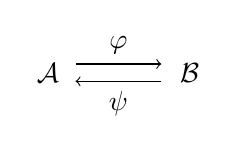
\begin{tikzpicture}[baseline]
\node (a) at (0,0) {\(\mathcal A\)};
\node (b) at (1.8,0) {\(\mathcal B\)};
\draw[->] (.35,.11)--(1.44,.11) node[midway,above] {\(\varphi\)};
\draw[->] (1.44,-.11)--(.35,-.11) node[midway,below] {\(\psi\)};
\end{tikzpicture}}\endgroup}
\end{GelfandAdjacentEvidence}
\begin{GelfandAdjacentEvidence}{GELFAND-P000721}{6}


\(\varphi,\psi\) --- функторы

\[
\varphi\circ\psi\underset{\uparrow}{\sim}\operatorname{id}_B,
\qquad
\psi\circ\varphi\underset{\nearrow}{\sim}\operatorname{id}_A
\]
[стрелки к обоим знакам из надписи] изоморфизм
\Incomplete{GELFAND-P000721}{bottom-cancellation}{Между «изоморфизм» и «функторов» густо зачёркнуто слово.}
\end{GelfandAdjacentEvidence}

функторов


\Needspace{7\baselineskip}
\begin{GelfandAdjacentEvidence}{GELFAND-P000722}{1}
\SourcePage{GELFAND-P000722}{61}
Изоморфизм функторов:
\[
\forall a:\qquad\psi\varphi(a)\longleftrightarrow a
\]
(не совпад., а изоморфно!)
и все диагр. коммутативны.

\uwave{Пример эквивал., но не изом. категорий:}

1) катег. конечномерных лин. пр-в над \(\mathbb C\)

2) --- ″ --- конечномерных модулей над \(M(2,\mathbb C)\).

Категория МХЧ [вставлено сверху в обводке: эквив.] нек-рой категории конечномерных модулей.
\Incomplete{GELFAND-P000722}{equiv-cancellation}{Под вставкой «эквив.» густо зачёркнуто слово.}
\end{GelfandAdjacentEvidence}
\begin{GelfandAdjacentEvidence}{GELFAND-P000722}{2}


\(\underset{\text{откр.}}{E}\subset\mathbb C^\ell\), \qquad \(B\) --- прям. сумма неск. матр. алгебр.
\Unclear{GELFAND-P000722}{dimension-ell}{Показатель при \(\mathbb C\) предположительно \(\ell\).}
\end{GelfandAdjacentEvidence}
\begin{GelfandAdjacentEvidence}{GELFAND-P000722}{3}


\(B(E)\) --- аналит. ф-и на \(E\) со знач. в \(B\)

\underline{\underline{Опр.}} Подалг. \(R\subset B(E)\) наз.
\uwave{приятной}, если

1) она сод. все скалярные ф-и:
\[
f(z)\mathbf 1_B\in R
\]

2) \(\{f(z), f\in R\}=B\) для почти всех \(z\in E\)

(т. е. для всех, кроме аналит. мн-ва меньшей размерности)

[зачёркнуто: Теорема?]
\Unclear{GELFAND-P000722}{theorem-cancellation}{Перечёркнутый заголовок предположительно «Теорема».}
\end{GelfandAdjacentEvidence}
\begin{GelfandAdjacentEvidence}{GELFAND-P000722}{4}

\(\operatorname{Mod} R\) --- катег. \(R\)-модулей, явл. конечномерными лин. пр-вами.

\underline{Теорема.}\qquad \(C_D\sim\operatorname{Mod} R\)

для нек-рой приятной алг. \(R\).

\(r\) --- ранг группы

\(\ell\) --- \uwave{расщепимый ранг группы}.
\Unclear{GELFAND-P000722}{split-rank}{Знак перед словами «расщепимый ранг» предположительно \(\ell\).}
\end{GelfandAdjacentEvidence}
\begin{GelfandAdjacentEvidence}{GELFAND-P000722}{5}


\begin{center}--- \(\cdot\) ---\end{center}
\uwave{Дальше всё будет на примере.}

\[
G=[\text{зачёркнуто }SL(2,\mathbb R)?]\quad SL_2(\mathbb R)/\{\pm1\},
\qquad
\underset{\text{алг. Ли}}{\mathfrak{sl}_2(\mathbb R)}=\{E_+,E_-,H\}
\]
\Unclear{GELFAND-P000722}{group-cancellation}{Зачёркнутая запись после \(G=\) предположительно \(SL(2,\mathbb R)\).}
\end{GelfandAdjacentEvidence}
\begin{GelfandAdjacentEvidence}{GELFAND-P000722}{6}

\[
Z(\mathfrak g)\ni 4E_-E_+-H^2+2H:=\Delta
\qquad
E_+=\begin{pmatrix}0&1\\0&0\end{pmatrix},\quad
E_-=\begin{pmatrix}0&0\\1&0\end{pmatrix},
\quad H=\begin{pmatrix}1&0\\0&-1\end{pmatrix}
\]
\Unclear{GELFAND-P000722}{casimir}{Перед \(H^2\) виден минус. Под знаком определения \(\Delta\) есть мелкие перечёркнутые штрихи.}
\end{GelfandAdjacentEvidence}
\begin{GelfandAdjacentEvidence}{GELFAND-P000722}{7}


Любой другой элемент \(Z(\mathfrak g)\) является полиномом
\Incomplete{GELFAND-P000722}{polynomial-cancellation}{После «полиномом» густо зачёркнута запись.}
\end{GelfandAdjacentEvidence}
\begin{GelfandAdjacentEvidence}{GELFAND-P000722}{8}

от \(\Delta\).

\(\Theta=\mathbb C^1\), \(D={}\) окрестность точки \(0\), дост. малая
\Unclear{GELFAND-P000722}{neighbourhood}{Знак после «точки» открыт справа и предположительно читается как 0.}
\end{GelfandAdjacentEvidence}


\uwave{Приятная подалгебра}:
\[
E=D,\qquad B=M_3(\mathbb C),\qquad
R\subset
\begin{pmatrix}
a_{11}(z)&a_{12}(z)&a_{13}(z)\\
\cdot&-&-\\
\cdot&-&-
\end{pmatrix}
=(a_{ij}(z))
\]


\Needspace{7\baselineskip}
\begin{GelfandAdjacentEvidence}{GELFAND-P000723}{1}
\SourcePage{GELFAND-P000723}{unlabelled}
\uwave{Условие, выделяющее \(R\):}
\[
a_{ij}(0)=
\begin{pmatrix}
\ast&0&0\\
\ast&\ast&0\\
\ast&0&\ast
\end{pmatrix}
\]

\uwave{Есть над ф-ями базис из 9 элементов.}
\[
e_{11}=
\begin{pmatrix}1&0&0\\0&0&0\\0&0&0\end{pmatrix},\quad
e_{12}
\begin{pmatrix}0&z&0\\0&0&0\\0&0&0\end{pmatrix},\quad
e_{21}=
\begin{pmatrix}0&0&0\\1&0&0\\0&0&0\end{pmatrix}
\]
и т. д.
\Unclear{GELFAND-P000723}{basis-e12-leading-zero}{В первом элементе матрицы при \(e_{12}\) нуль обведён густыми штрихами.}
\end{GelfandAdjacentEvidence}
\begin{GelfandAdjacentEvidence}{GELFAND-P000723}{2}

\Unclear{GELFAND-P000723}{basis-e12-gap}{Между \(e_{12}\) и открывающей скобкой знак равенства не виден.}
\end{GelfandAdjacentEvidence}
\begin{GelfandAdjacentEvidence}{GELFAND-P000723}{3}


\begin{center}
\begingroup\color{black}\GelfandFitDiagram{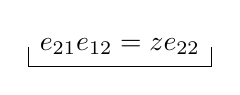
\begin{tikzpicture}
\node (product) [inner sep=4pt] {\(e_{21}e_{12}=ze_{22}\)};
\draw (product.west)--(product.south west)--(product.south east)--(product.east);
\end{tikzpicture}}\endgroup
\end{center}

Хотим найти конечномерные модули, чтобы умн. на \(z\) было нильпот. оператором.
\[
\underline{e_{ii}^{2}=e_{ii}}.
\]
\[
L_i=\{m:\ e_{ii}m=m\}.
\]
\[
M=L_1\oplus L_2\oplus L_3
\]

\SourceFigure{GELFAND-P000723}{diagram-right-directions}{%
\par\begingroup\color{black}\GelfandFitDiagram{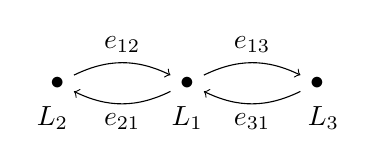
\begin{tikzpicture}[baseline,x=1cm,y=.92cm]
\node (l2) at (0,0) {\(\bullet\)};
\node (l1) at (1.65,0) {\(\bullet\)};
\node (l3) at (3.30,0) {\(\bullet\)};
\node at (-.06,-.48) {\(L_2\)};
\node at (1.65,-.48) {\(L_1\)};
\node at (3.38,-.48) {\(L_3\)};
\draw[->] (l2) to[bend left=26] node[above] {\(e_{12}\)} (l1);
\draw[->] (l1) to[bend left=26] node[below] {\(e_{21}\)} (l2);
\draw[->] (l1) to[bend left=26] node[above] {\(e_{13}\)} (l3);
\draw[->] (l3) to[bend left=26] node[below] {\(e_{31}\)} (l1);
\end{tikzpicture}}\endgroup\par\smallskip
На оригинале стрелка \(e_{13}\) идёт от \(L_1\) к \(L_3\), а \(e_{31}\) от \(L_3\) к \(L_1\).}
\end{GelfandAdjacentEvidence}


\[
e_{21}e_{12}=ze_{22}\qquad\text{нильпотентен}
\]
\[
e_{12}e_{21}=ze_{11}=e_{13}e_{31}
\]
отсюда катег. модулей над этим кольцом \(\cong\ldots\)

\underline{\uwave{Для \(SL(3,\mathbb R)\)}}\qquad
\uwave{ответ таков:}
\[
E=\{z_1,z_2\}\qquad\text{в окр. нуля:}
\]
\[
B=\underset{a_{ij}}{M_4}\oplus
\underset{b_{ij}}{M_3}\oplus
\underset{c_{ij}}{M_3}\oplus
\underset{d}{M_1}
\]
\underline{Условия.}
\[
1)\ \text{При }z_1=0\qquad\left\Vert\quad
\begin{aligned}
a_{13}=a_{14}=a_{23}=a_{24}=b_{12}=b_{13}=0\\
a_{33}=b_{22},\quad a_{34}=b_{23},\quad
a_{43}=b_{32},\quad a_{44}=b_{33}
\end{aligned}\right.
\]


\Needspace{7\baselineskip}
\begin{GelfandAdjacentEvidence}{GELFAND-P000724}{1}
\SourcePage{GELFAND-P000724}{62}
\SourceFigure{GELFAND-P000724}{top-matrix-consistency}{%
\begingroup\color{black}\GelfandFitDiagram{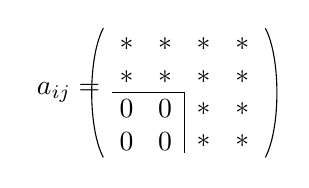
\begin{tikzpicture}[baseline=(current bounding box.center),x=.49cm,y=.41cm]
\node at (-1.5,-1.5) {\(a_{ij}=\)};
\foreach \row in {0,1} {
  \foreach \col in {0,1,2,3} {\node at (\col,-\row) {\(\ast\)};}
}
\foreach \row in {2,3} {
  \foreach \col in {0,1} {\node at (\col,-\row) {\(0\)};}
  \foreach \col in {2,3} {\node at (\col,-\row) {\(\ast\)};}
}
\draw (-.6,.5) .. controls (-1,-.4) and (-1,-2.6) .. (-.6,-3.5);
\draw (3.6,.5) .. controls (4,-.4) and (4,-2.6) .. (3.6,-3.5);
\draw (-.38,-1.5)--(1.5,-1.5)--(1.5,-3.35);
\end{tikzpicture}}\endgroup}
\end{GelfandAdjacentEvidence}
\begin{GelfandAdjacentEvidence}{GELFAND-P000724}{2}

\SourceFigure{GELFAND-P000724}{top-matrix-consistency-right}{%
\begingroup\color{black}\GelfandFitDiagram{\begin{tikzpicture}\node[inner sep=0pt] {\(\begin{pmatrix}\ast&\ast&\ast\\0&\ast&\ast\\0&\ast&\ast\end{pmatrix}\)};\end{tikzpicture}}\endgroup}
\end{GelfandAdjacentEvidence}
\begin{GelfandAdjacentEvidence}{GELFAND-P000724}{3}


\[
2)\ \text{При }z_2=0\qquad\left\Vert\quad
\begin{aligned}
a_{12}=a_{14}=a_{34}=c_{12}=c_{13}=a_{32}=0\\
a_{22}=c_{22},\quad a_{24}=c_{23},\quad
a_{42}=c_{32},\quad a_{44}=c_{33}
\end{aligned}\right.
\]

\[
3)\ \text{При }z_1+z_2=0.\qquad\left\Vert\quad
\begin{aligned}
b_{13}=b_{23}=c_{13}=c_{23}=0;\\
b_{33}=c_{33}.
\end{aligned}\right.
\]
\Unclear{GELFAND-P000724}{condition-three-sign}{Переписанный знак между \(z_1\) и \(z_2\) предположительно читается как \(+\).}
\end{GelfandAdjacentEvidence}



\Needspace{7\baselineskip}
\begin{GelfandAdjacentEvidence}{GELFAND-P000725}{1}
\SourcePage{GELFAND-P000725}{unlabelled}
\underline{24/X--77 г.}

\underline{С. И. Гельфанд.}\qquad\underline{Модули Хариш--Чандры}

МХЧ для
\[
\begin{aligned}
G&=SL(2,\mathbb R)/(\pm1)\\
K&=SO_2/(\pm1)\\[-.25ex]
 &\quad\text{(макс. комп. подгруппа)}
\end{aligned}
\]

\(\mathfrak g\) --- алгебра Ли
\[
\begin{array}{ccc}
E_+,&E_-,&H\\[.4ex]
\begin{pmatrix}0&1\\0&0\end{pmatrix},&
\begin{pmatrix}0&0\\1&0\end{pmatrix},&
\begin{pmatrix}1&0\\0&-1\end{pmatrix}
\end{array}
\qquad\text{--- образующие }\mathfrak g
\]
\[
\begin{array}{cl}
\mathfrak k&\subset\mathfrak g.\\[-.5ex]
\Vert&\\
\multicolumn{2}{l}{\left\{\begin{pmatrix}0&1\\-1&0\end{pmatrix}=X_c\right\}}
\end{array}
\]
\Unclear{GELFAND-P000725}{bottom-generator}{Подстрочный знак при \(X\) читается как открытая \(c\).}
\end{GelfandAdjacentEvidence}



\Needspace{7\baselineskip}
\begin{GelfandAdjacentEvidence}{GELFAND-P000726}{1}
\SourcePage{GELFAND-P000726}{67}
\uwave{Модуль} Х.--Ч. --- такое (бесконечномерное) предст. в [зачёркнуто] \(V\), что
\Unclear{GELFAND-P000726}{top-cancellation}{Зачёркнутый фрагмент перед \(V\) не читается.}
\end{GelfandAdjacentEvidence}
\begin{GelfandAdjacentEvidence}{GELFAND-P000726}{2}


1) \(X_0\) имеет лишь целочисленные соб. значения и притом чётные

2) [зачёркнуто] каждое собств. значение [вписано сверху: оператора \(X_0\)] конечнократно
\Unclear{GELFAND-P000726}{item-two-cancellation}{Густо зачёркнутый знак после номера 2) не читается.}
\end{GelfandAdjacentEvidence}
\begin{GelfandAdjacentEvidence}{GELFAND-P000726}{3}


3) \(V\) конечно порождён (над обёрт. алгеброй)

(\(\Leftrightarrow\) кратности соб. значений ограничены).

\(v_1,\ldots,v_n\) --- образующие

\begin{quote}
\small \textit{[На правом поле за двойной чертой]} 1) --- чтобы можно было проинтегрировать до предст. группы (\(e^{inx}\) и т. д.)
\end{quote}

\uwave{Определение.}\quad \(Z(\mathfrak g)\) --- центр обёрт. алгебры \(U(\mathfrak g)\)

(порожд. элементом \(z=4E_-E_+-H^2+2H\))
\Unclear{GELFAND-P000726}{casimir-sign}{В рукописи перед \(H^2\) стоит минус, а перед \(2H\) --- плюс.}
\end{GelfandAdjacentEvidence}
\begin{GelfandAdjacentEvidence}{GELFAND-P000726}{4}


\(\operatorname{supp} V={}\) мн-во собств. значений оператора \(z\) в \(V\)

\underline{Теорема:} это конечное мн-во для любого \(V\).

\uwave{Определение.} Пусть \(D\) --- область в \(\mathbb C\).
\[
C_D=\{V,\ \operatorname{supp}V\subset D\}
\]
Пусть \(D\) --- маленькая окрестность нуля (круг радиуса \(<1/2\)).
\[
R=\left\{\begin{pmatrix}
a_{11}(\lambda)&a_{12}(\lambda)&a_{13}(\lambda)\\
a_{21}(\lambda)&a_{22}(\lambda)&a_{23}(\lambda)\\
a_{31}(\lambda)&a_{32}(\lambda)&a_{33}(\lambda)
\end{pmatrix}\right.,\quad a_{ij}(\lambda)\text{ --- аналит. ф-и в }D
\]
\Unclear{GELFAND-P000726}{matrix-index-overwrite}{Первый знак индекса при \(a_{12}(\lambda)\) переписан, читается как \(1\).}
\end{GelfandAdjacentEvidence}
\begin{GelfandAdjacentEvidence}{GELFAND-P000726}{5}


\[
a_{ij}(0)=\begin{pmatrix}\ast&0&0\\\ast&\ast&0\\\ast&0&\ast\end{pmatrix}
\]
\Unclear{GELFAND-P000726}{matrix-value-notation}{Слева от равенства написано \(a_{ij}(0)\).}
\end{GelfandAdjacentEvidence}
\begin{GelfandAdjacentEvidence}{GELFAND-P000726}{6}


\[
\operatorname{Mod} R=
\left\{\underset{\substack{|\\R\text{-модуль}}}{M}:\ \dim_{\mathbb C}M<\infty\right\}
\]
\underline{Теорема.} Категория \(C_D\) эквивалентна категории \(\operatorname{Mod} R\).

\underline{Пример.}

\uwave{Категория модулей над кольцом матриц эквивалентна категории} [зачёркнуто: линей\ldots?] \uwave{конечномерных линейных пространств}
\Unclear{GELFAND-P000726}{cancelled-category}{Начало зачёркнутого слова предположительно читается как «линей»; конец не установлен.}
\end{GelfandAdjacentEvidence}
\begin{GelfandAdjacentEvidence}{GELFAND-P000726}{7}


(\(\sim\) предст. алг. матриц --- прямая сумма)

\(V\) --- станд. предст. алг. \(M_\ell\)
\Unclear{GELFAND-P000726}{matrix-subscript}{Индекс при \(M\) предположительно читается как \(\ell\); знак также похож на \(e\).}
\end{GelfandAdjacentEvidence}

\[
E\longmapsto V\underset{\mathbb C}{\otimes}E,\qquad
M_\ell\text{ действ. по 1-му переменному}
\]
\[
W\text{ --- }M_\ell\text{-модуль}\quad\longmapsto\quad
E=\operatorname{Hom}_{M_\ell}(V,W).
\]
(выписаны 2 функтора, задающие эквивалентность)

Старая формулировка: \(\forall\, M_\ell\) модуль разлагается в прямую сумму.


\Needspace{7\baselineskip}
\begin{GelfandAdjacentEvidence}{GELFAND-P000727}{1}
\SourcePage{GELFAND-P000727}{unlabelled}
\underline{Док-во теоремы.}

I. Пусть дан набор чисел \(n_1,\ldots,n_k\). Построим по нему кольцо \(Q_{n_1,\ldots,n_k}\)

а) \(J_{n_1\ldots n_k}\) --- левый идеал в \(U(\mathfrak g)\), порождённый элементом
\[
(X_0-2in_1)(X_0-2in_2)\cdots(X_0-2in_k)
\]

\[
\text{б)}\quad
N_{n_1,\ldots,n_k}=
\{u\in U(\mathfrak g)\mid
J_{n_1,\ldots,n_k}u\subset J_{n_1,\ldots,n_k}\}
\]
(наименьшая подалг., в к-рой \(J\) --- 2-стор. идеал
\Unclear{GELFAND-P000727}{normalizer-word}{В рукописи читается «наименьшая».}
\end{GelfandAdjacentEvidence}
\begin{GelfandAdjacentEvidence}{GELFAND-P000727}{2}


\[
Q_{n_1\ldots n_k}=N_{n_1,\ldots,n_k}/J_{n_1,\ldots,n_k}
\]

\uuline{Опред.}\quad \(V\) --- модуль Х.--Ч.
\[
\tau_{n_1,\ldots,n_k}(V)\underset{\mathrm{def}}{=}
\{v:\ (X_0-2in_1)\cdots(X_0-2in_k)v=0\}
\]

Это конечномерное подпр-во

Размерность \(={}\) сумме кратностей

\(N\) переводит его в себя

\(J\)\quad --- '' --- \quad в нуль
\[
\Rightarrow\quad Q_{n_1,\ldots,n_k}\text{ действует в }\tau_{n_1,\ldots,n_k}(V)
\]

Это [зачёркнуто: конструкция?], функтор
\Unclear{GELFAND-P000727}{functor-cancellation}{Зачёркнутое слово предположительно «конструкция».}
\end{GelfandAdjacentEvidence}
\begin{GelfandAdjacentEvidence}{GELFAND-P000727}{3}

\[
\text{Модули Х.--Ч.}\longrightarrow
\text{конечномерные модули над }Q_{n_1,\ldots,n_k}
\]
\Unclear{GELFAND-P000727}{overwritten-functor-subscript}{Первый знак последнего индекса у \(Q\) обведён. Читается \(n_k\).}
\end{GelfandAdjacentEvidence}
\begin{GelfandAdjacentEvidence}{GELFAND-P000727}{4}


Ясно, что
\[
z\in N_{n_1,\ldots,n_k}
\]
\[
\operatorname{supp} M=\{\text{соб. значения }z\}
\]
\[
(\operatorname{Mod} Q_{n_1,\ldots,n_k})_D
\]
(конечномерные модули с носителем в \(D\)).

\SourceFigure{GELFAND-P000727}{bottom-arrow}{%
\par\begingroup\color{black}\GelfandFitDiagram{\begin{tikzpicture}[baseline=(current bounding box.center)]
\draw[<-] (0,0)--(.8,0);
\draw (.8,-.15)--(.8,.15);
\end{tikzpicture}}\endgroup\par\smallskip
Короткая стрелка направлена влево. Справа видна поперечная черта. Связь с соседней строкой неясна.}
\end{GelfandAdjacentEvidence}


\uwave{Теорема} 1. Пусть \(D\) --- любая огр. область в \(\mathbb C^1\).
Тогда сущ. \(n_1,\ldots,n_k\), такие что \(C_D\) и
\((\operatorname{Mod} Q_{n_1,\ldots,n_k})_D\) эквив.


\Needspace{7\baselineskip}
\begin{GelfandAdjacentEvidence}{GELFAND-P000728}{1}
\SourcePage{GELFAND-P000728}{68}
\underline{II.}\quad \underline{Определение предст. основной серии.}

по \(s\) постр. модуль \(T^{(s)}=V\)
\[
V=\{\underset{\substack{\text{функции}\\\text{на плоск.}}}{f(x,y)}\}
\]
1) \(f(tx,ty)=|t|^sf(x,y)\)

2) \(f(+\sin\varphi,\cos\varphi)=P(\sin\varphi,\cos\varphi)\)
\Unclear{GELFAND-P000728}{plus-sine}{Перед \(\sin\varphi\) в первом аргументе стоит \(+\).}
\end{GelfandAdjacentEvidence}
\begin{GelfandAdjacentEvidence}{GELFAND-P000728}{2}


\(\underline{P}\) --- многочлен.

Алгебра Ли действ. естеств. образом (дифф. операторы)

(группа --- на аргумент)
\[
E_+\sim x\frac{\partial}{\partial y};\quad
E_-\sim y\frac{\partial}{\partial x};\quad
H\sim x\frac{\partial}{\partial x}-y\frac{\partial}{\partial y}.
\]
Огранич. на \(S^1\cong{}\) пр-во многочленов (чётных на окружности)
\[
L_0\simeq T^{(s)}\qquad\text{(при любом }s\text{).}
\]
\Unclear{GELFAND-P000728}{l0-degree}{Открывающая скобка в показателе \((s)\) обведена густо.}
\end{GelfandAdjacentEvidence}
\begin{GelfandAdjacentEvidence}{GELFAND-P000728}{3}


\underline{Лемма 1.} Пусть \(X\in U(\mathfrak g)\). Действие \(X\) полиномиально зависит от \(s\).

(Матричные элементы в базисе одночленов --- полиномы от \(s\))
\[
\tau_{n_1,\ldots,n_k}(T^{(s)})=L_{n_1,\ldots,n_k}
\]
\underline{Лемма 2.} Пусть \(q\in Q_{n_1,\ldots,n_k}\). Действие \(q\) полиномиально зависит от \(s\).

\uwave{Теорема 2.}\quad \uwave{Положим}
\[
B_{n_1,\ldots,n_k}=\operatorname{End}(L_{n_1,\ldots,n_k})
\]
Тогда существует отображение
\[
\psi_{n_1,\ldots,n_k}:
Q_{n_1,\ldots,n_k}\longrightarrow B_{n_1,\ldots,n_k}[s],
\]
\Unclear{GELFAND-P000728}{embedding-symbol}{Знак отображения предположительно \(\psi\).}
\end{GelfandAdjacentEvidence}
\begin{GelfandAdjacentEvidence}{GELFAND-P000728}{4}


[зачёркнуто: Теор.?] [вставлено сверху: так что] \(\psi\) --- \uwave{вложение}
\Unclear{GELFAND-P000728}{embedding-cancellation}{Зачёркнутый заголовок предположительно читается «Теор.».}
\end{GelfandAdjacentEvidence}
\begin{GelfandAdjacentEvidence}{GELFAND-P000728}{5}


(т. е. в основной серии в кач. под- и фактор- предст. содерж. \(\forall\) МХЧ)

\underline{III.}\quad \uwave{Объед. I и II этапов.}

\(D\) --- маленькая окр. нуля

\underline{Лемма 0.}

На \(T^{(s)}\) оператор \(z\) есть \((-s^2+2s)\operatorname{Id}\)
\Unclear{GELFAND-P000728}{scalar-casimir}{В рукописи написано \((-s^2+2s)\operatorname{Id}\).}
\end{GelfandAdjacentEvidence}
\begin{GelfandAdjacentEvidence}{GELFAND-P000728}{6}


\(z=0\) при \(s=0\) и \(s=2\).

\underline{Лемма 1.} Пусть \(s\) вблизи точки 0.

1) Тогда \(T^s\), \(s\ne 0\) неприводимо
\[
0\longrightarrow\operatorname{Id}\longrightarrow T^{(0)}
\longrightarrow T_+\oplus T_-\longrightarrow 0
\]
\Unclear{GELFAND-P000728}{identity-overtrace}{В обозначении \(\operatorname{Id}\) вторая буква густо обведена.}
\end{GelfandAdjacentEvidence}

и точн. послед. не расщепляется


\Needspace{7\baselineskip}
\begin{GelfandAdjacentEvidence}{GELFAND-P000729}{1}
\SourcePage{GELFAND-P000729}{unlabelled}
\[
2)\quad T^{(s)}\big|_K=\bigoplus_{j=-\infty}^{\infty}\delta_j.
\]
\(\delta_k={}\) соб. подпр. \(X_0\) с соб. знач. \(2ik\).

(1-мерное предст.)
\[
I\big|_K=\delta_0,\qquad
T_+\big|_K=\bigoplus_{j>0}\delta_j,\qquad
T_-\big|_K=\bigoplus_{j<0}\delta_j.
\]
\Unclear{GELFAND-P000729}{right-edge-mark}{За правой границей листа виден узкий знак, похожий на \(I\). Его связь с записью не установлена.}
\end{GelfandAdjacentEvidence}
\begin{GelfandAdjacentEvidence}{GELFAND-P000729}{2}


[На левом поле: В?] \underline{Лемма 2.} Вблизи \(s=2\)
\Unclear{GELFAND-P000729}{lemma-margin-letter}{Густо обведённый знак на поле предположительно читается «В».}
\end{GelfandAdjacentEvidence}
\begin{GelfandAdjacentEvidence}{GELFAND-P000729}{3}

\[
0\longrightarrow T_+\oplus T_-\longrightarrow T^{(2)}\longrightarrow I\longrightarrow0
\]
\(T^{(s)}\), \(s\ne2\) неприводимо

\underline{Лемма 3.}\quad \(s\ne0\qquad T^{(s)}\simeq T^{(2-s)}\)

\(s\) вблизи нуля
\Unclear{GELFAND-P000729}{lemma-three-superscript}{Открывающая скобка показателя в \(T^{(s)}\) обведена.}
\end{GelfandAdjacentEvidence}
\begin{GelfandAdjacentEvidence}{GELFAND-P000729}{4}


Рассмотрим числа \((n_1,n_2,n_3)=(-1,0,1)\) и кольцо
\[
Q_{(-1,0,1)}
\]
\(D\) --- дост. малая окр. нуля \(\qquad\Rightarrow\quad C_D\sim Q_{(-1,0,1)}\)

(\underline{объяснение:} в \(T_+\) есть предст. с \(+1\), в \(T_-\) --- '' --- с \(-1\) и т. д.)
\[
\tau_{-1,0,1}(T^{(s)})=\{e_{-1},e_0,e_1\}
\]
\(q\in Q_{-1,0,1}\)

\par\smallskip\noindent\dotfill\par\smallskip

\underline{Сделано}:\quad \(SL(2,\mathbb R)/(\pm1)\), \(SL(2,\mathbb R)\), \(PGL(2,\mathbb R)\),

\(SL(2,\mathbb C)\), \(SL(3,\mathbb R)\)

Наверное, можно \(SL(3,\mathbb C)\) и \(SU(2,1)\)

Рекомендуется, сосчит. \(SO(4,1)\) (легко), \(Sp(4,\mathbb C)\) (легко)

Трудно: \(SL(4,\mathbb R)/(\pm1)\), \(SL(4,\mathbb C)\).

Читать: раб. Хираи; Желобенко

Гельфанд, Граев

\underline{Кричевер}

\uwave{2 минуты для сенсационного сообщения.}

[На левом поле: \uwave{Об ур-и?}]
\[
[L_1,L_2]=0
\]
\Unclear{GELFAND-P000729}{margin-abbreviation}{Сокращение предположительно читается «Об ур-и», возможно «Об ур-й».}
\end{GelfandAdjacentEvidence}
\begin{GelfandAdjacentEvidence}{GELFAND-P000729}{5}


Коддингтон указал на раб.

\uwave{Burchnal}, \uwave{Chaundy}\quad
\href{https://doi.org/10.1112/plms/s2-21.1.420}{1922},
\href{https://doi.org/10.1098/rspa.1928.0069}{1928},
\href{https://doi.org/10.1098/rspa.1931.0208}{1931}

и \uwave{Baker} [зачёркнуто] \href{https://doi.org/10.1098/rspa.1928.0070}{1928}
\Unclear{GELFAND-P000729}{baker-cancellation}{Запись между «Baker» и «1928» густо зачёркнута.}
\end{GelfandAdjacentEvidence}


[Справа от списка работ:] --- возразили Baker'у, к-рый рекомендовал польз. алг. геом.

Поставлена и решена задача об описании коммут. опр. со скал. коэфф. взаимно простого пор.

ответ не через \(\Theta\)-ф-и и не достаточно эффективен

1-й через ф-и Ламе нашли (как Ахиезер). не увидели прямолин.


\Needspace{7\baselineskip}
\begin{GelfandAdjacentEvidence}{GELFAND-P000730}{1}
\SourcePage{GELFAND-P000730}{69}
пути на якобиане (и даже условной периодичности).

Забыли --- в раб. 1939 ссылок уже нет.

\SourceFigure{GELFAND-P000730}{proceedings-brackets}{%
\par\begingroup\color{black}\GelfandFitDiagram{\begin{tikzpicture}[x=1cm,y=1cm]
\foreach \x in {0,1.08} {
 \draw (\x,-.43) rectangle ++(.08,.86);
 \draw (\x-.07,.43)--++(.23,0) (\x-.07,-.43)--++(.23,0);
 \foreach \y in {-.35,-.24,-.13,-.02,.09,.20,.31}
  {\draw (\x,\y)--++(.08,.05);}
}
\node[anchor=west,inner sep=0pt] at (.23,.25) {Proc.};
\node[anchor=west,inner sep=0pt] at (.23,-.26) {Proc.};
\node[anchor=west,inner sep=0pt,text=black] at (1.28,.25)
  {Lond. Math. Soc. \href{https://doi.org/10.1112/plms/s2-21.1.420}{1922}.};
\node[anchor=west,inner sep=0pt,text=black] at (1.28,-.26)
  {Royal Soc. --- остальные};
\end{tikzpicture}}\endgroup\par}
\end{GelfandAdjacentEvidence}
\begin{GelfandAdjacentEvidence}{GELFAND-P000730}{2}


почти коммутир. [зачёркнуто] и пары Лакса \uuline{есть}.
\Unclear{GELFAND-P000730}{lax-cancellation}{После «коммутир.» зачёркнут небольшой знак.}
\end{GelfandAdjacentEvidence}
\begin{GelfandAdjacentEvidence}{GELFAND-P000730}{3}


[зачёркнуто] \underline{31/X--77 г.}\quad \underline{Сем. Гельфанда.}\quad
\uuline{С. П. Новиков.}\quad \uuline{Инстантоны.}
\Unclear{GELFAND-P000730}{date-cancellation}{Густо зачёркнутый знак перед датой не читается.}
\end{GelfandAdjacentEvidence}
\begin{GelfandAdjacentEvidence}{GELFAND-P000730}{4}


\[
\mathbb R^4\subset S^4\qquad(|x|\to\infty)
\]
\[
A=\text{[зачёркнуто]}\ A_\mu\,dx^\mu
\qquad\text{форма связности}
\]
\Unclear{GELFAND-P000730}{connection-cancellation}{В зачёркнутом фрагменте после \(A=\) предположительно видны \(A\) и \(d\). Индексы не читаются.}
\end{GelfandAdjacentEvidence}
\begin{GelfandAdjacentEvidence}{GELFAND-P000730}{5}


Если кривизна равна 0, то
\[
(1)\qquad A_\mu\longrightarrow\frac{\partial g}{\partial x^\mu}\,g^{-1}(x),
\qquad g(x)\in G
\]
\[
A_\mu(x)\in L_G\qquad\text{(алгебра Ли)}
\]
Форма кривизны:
\[
(2)\qquad F_{\nu\mu}=dA+[A,A]=\mathcal D A
\]
(ковариантная производная)

Чаще всего \(G=SU_2\) (Янг--Миллс).

\([A,A]\) --- внешнее произв., но умн. коэфф. --- в алг. Ли.

Другие обозначения: \(A\wedge A=[A,A]\), \(\mathcal D A=\nabla_A A\)

Требование, что всё на \(S^4\) --- чуть сильнее конечности энергии.

(\underline{Замеч.} Нелинейные (киральные) поля \(\leftrightarrow\) связность с 0-й кривизной;
задаётся ф-ями со знач. в группе.)

Положим
\[
(3)\qquad n=P(A)=\frac12\int\varepsilon_{abcd}F^{ab}F^{cd}\,d^4x
\]
\Unclear{GELFAND-P000730}{topological-integral}{В (3) перед произведением \(F^{ab}F^{cd}\) обозначение следа не написано.}
\end{GelfandAdjacentEvidence}
\begin{GelfandAdjacentEvidence}{GELFAND-P000730}{6}

(хар. класс Черна --- топ. инвариант --- целое число с точн. до множителя \(\frac{\pi^2}{16}\)).
\Unclear{GELFAND-P000730}{chern-factor}{Знаменатель дроби предположительно читается как \(16\).}
\end{GelfandAdjacentEvidence}
\begin{GelfandAdjacentEvidence}{GELFAND-P000730}{7}


\[
(4)\qquad S(A)=\frac1{g_c}\int_{\mathbb R^4}
       \operatorname{Sp}(F_{\mu\nu}F^{\mu\nu})\,d^4x
\]
\Unclear{GELFAND-P000730}{coupling-subscript}{Разомкнутый нижний индекс при \(g\) предположительно \(c\), возможно \(0\).}
\end{GelfandAdjacentEvidence}
\begin{GelfandAdjacentEvidence}{GELFAND-P000730}{8}

(ф-л Янга--Миллса)

\uwave{Классич. эл.-динамика} --- \(G=SU(1)\) или \(\mathbb R\)
\Unclear{GELFAND-P000730}{electrodynamics-group}{В рукописи написано \(SU(1)\).}
\end{GelfandAdjacentEvidence}
\begin{GelfandAdjacentEvidence}{GELFAND-P000730}{9}


в завис. от того, есть ли реал. заряды или нет.
\Unclear{GELFAND-P000730}{charges-adjective}{Бледное сокращение перед «заряды» предположительно читается «реал.».}
\end{GelfandAdjacentEvidence}


Ур-я Янга--Миллса:
\[
(5)\qquad \delta S=0.
\]
Классич. задача: найти все такие \(A\), что \(S(A)<+\infty\).

\underline{Замеч.} Метрика \(S^4\) конформно эквив. метрике \(\mathbb R^4\),
\[
g_{\mu\nu}(y)=g(y)\delta_{\mu\nu}
\]
Ур-я Максвелла и Янга--Миллса \uwave{конформно инвариантны}.

Гр. конформных преобр. евкл. пр-ва и сферы \(\qquad\Vert\qquad O(5,1)=K_4\)


\Needspace{7\baselineskip}
\begin{GelfandAdjacentEvidence}{GELFAND-P000731}{1}
\SourcePage{GELFAND-P000731}{unlabelled}
Решения умн. на скаляр под действ. конформной группы:
\[
f:X\longrightarrow X,\qquad f^*(g_{ij})=g(x)g_{ij}.
\]
(непрерывные конф. преобр.)
\Unclear{GELFAND-P000731}{parenthesis-word}{Первое слово в скобках предположительно читается «непрерывные».}
\end{GelfandAdjacentEvidence}
\begin{GelfandAdjacentEvidence}{GELFAND-P000731}{2}


[зачёркнуто: Непр. рассл. в?]
\Unclear{GELFAND-P000731}{top-cancellation}{В зачёркнутой строке предположительно «Непр. рассл. в».}
\end{GelfandAdjacentEvidence}
\begin{GelfandAdjacentEvidence}{GELFAND-P000731}{3}


Непр. отобр. баз переводит рассл. в рассл. и связность в связность.
Тогда новая связность снова удовл. ур-ю Янга--Миллса.

\(\underline{\underline{O(5,1)}}\)

На сфере \(S^4\) есть \(O(5)\)

Стереогр. преобр. \(S^4\) на \(\mathbb R^4\) и в \(\mathbb R^4\) берём подобные преобр..

Откуда \(O(5,1)\)?

Надо рассм. конус
\[
\underline{x_1^2+x_2^2+\cdots+x_5^2-x_6^2=0.}
\]
\SourceFigure{GELFAND-P000731}{null-cone-diagram}{%
\par\begingroup\color{black}\GelfandFitDiagram{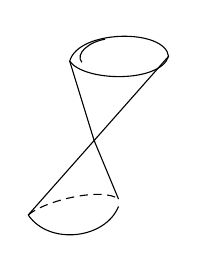
\begin{tikzpicture}[x=1.55cm,y=1.55cm]
\draw (-.20,.65) .. controls (-.13,.91) and (.58,.92) .. (.61,.69)
 .. controls (.54,.47) and (-.08,.48) .. (-.20,.65);
\draw (-.10,.64) .. controls (-.16,.71) and (-.04,.81) .. (.09,.83);
\draw (-.20,.65)--(0,0)--(.20,-.48);
\draw (.61,.69)--(0,0)--(-.54,-.61);
\draw (-.54,-.61) .. controls (-.37,-.86) and (.09,-.81) .. (.20,-.54);
\draw[densely dashed] (-.54,-.61) .. controls (-.40,-.49) and (.07,-.38) .. (.20,-.48);
\end{tikzpicture}}\endgroup\par}
\end{GelfandAdjacentEvidence}
\begin{GelfandAdjacentEvidence}{GELFAND-P000731}{4}

[неразобранный знак] и лин. преобр., сохр. конус.
\Unclear{GELFAND-P000731}{cone-caption-symbol}{Отдельный знак перед «и» не удалось прочитать.}
\end{GelfandAdjacentEvidence}
\begin{GelfandAdjacentEvidence}{GELFAND-P000731}{5}


Лучи конуса --- \(S^4\). Преобр. конформные на \(S^4\).

Конформная группа сохр. ф-л \(S(A)\)

\uwave{Инстантоны Белавина--Полякова.}
\[
(6)\qquad \min_{P(A)=n}S(A)=n.\qquad \text{(при }g_c=1\text{)}
\]
\Unclear{GELFAND-P000731}{coupling-condition}{Нижний индекс при \(g\) предположительно \(c\), возможно \(0\).}
\end{GelfandAdjacentEvidence}
\begin{GelfandAdjacentEvidence}{GELFAND-P000731}{6}


и на самом деле минимумы удовл. ур-ю [зачёркнуто]
\Unclear{GELFAND-P000731}{equation-cancellation}{Зачёркнутая запись похожа на \(F={*}F\); средние знаки не читаются уверенно.}
\end{GelfandAdjacentEvidence}
\begin{GelfandAdjacentEvidence}{GELFAND-P000731}{7}

\[
(7)\qquad \underline{F={*}F}
\]
(ур-я дуальности)

(\href{https://doi.org/10.1016/0370-2693(75)90163-X}{Белавин и Поляков})

И обратное, реш. этих ур-й с данным \(n\) --- реализ. строгий минимум в данном классе.

Явно представили ряд авторов (для \(\forall\,n\) хотя бы сущ. решение).

[зачёркнуто: Гер?] \underline{t' Hooft} нашёл явные ф-лы при \(\underline{n=2}\). (все решения!)
\Unclear{GELFAND-P000731}{hooft-cancellation}{Зачёркнутый фрагмент перед фамилией предположительно читается «Гер».}
\end{GelfandAdjacentEvidence}
\begin{GelfandAdjacentEvidence}{GELFAND-P000731}{8}


с пом. элем. подстановки.

Решения обр. \((8n-3)\)-мерное многообразие
(Шварц из теор. Атьи--Зингера). Это \(M^{8n-3}\).

Атья--Зингер на 3 месяца позже.

t' Hooft нашёл [зачёркнуто] мн-ие размерности \(\underline{\underline{5n+4}}\). (\(n\geq3\))
\Unclear{GELFAND-P000731}{family-cancellation}{Короткая зачёркнутая запись после «нашёл» не читается.}
\end{GelfandAdjacentEvidence}
\begin{GelfandAdjacentEvidence}{GELFAND-P000731}{9}


При \(n=2\) совпадают. Не ясно, нет ли ещё связной компоненты.

\underline{Д-во теор. Шварца}

Линеаризуем ур-я (7):
\[
(A_\mu)\longrightarrow A_\mu+a_\mu=A+\delta A
\]
линеариз. оператор\quad \(a_\mu\longrightarrow Ta_\mu\)
\Unclear{GELFAND-P000731}{final-speck}{Справа от \(Ta_\mu\) виден отдельный неразобранный след.}
\end{GelfandAdjacentEvidence}



\Needspace{7\baselineskip}
\begin{GelfandAdjacentEvidence}{GELFAND-P000732}{1}
\SourcePage{GELFAND-P000732}{70}
\[
\begin{aligned}
B(A)&=F-{*}F=0,\\
B(A+\delta A)&=T(\delta A)+O((\delta A)^2)
\end{aligned}
\]
\uwave{Счёт индекса}: \(cn\) --- линейная ф-я от \(n\); считаются знач. в \(0\) и \(1\).

\uuline{Коядро \(=0\)}\quad [зачёркнуто]\quad \(\Leftarrow\) хопфевы соображения.
\Unclear{GELFAND-P000732}{index-cancellation}{После «Коядро = 0» густо зачёркнут фрагмент. Справа видна стрелка влево.}
\end{GelfandAdjacentEvidence}
\begin{GelfandAdjacentEvidence}{GELFAND-P000732}{2}


Получ. \(\underline{\underline{8n}}\): 3 параметра лишних из калибр. \underline{инвариантности}.

Исп. конф. группы \(\Rightarrow\) При \(n=1\) все реш. сферич. симметричны.

\(O(5,1)\) действует на мн-ве реш.

\uwave{При \(n=1\) мн-во реш. 5-мерн.}\qquad [Справа:] \(\dim O(5,1)=15\).

на \(\forall\) связн. комп. действ. \(O(5,1)\).

Поэтому стац. подгруппа имеет разм. \(\geq10\). Но \(>10\) не бывает, т.к. стац. подгруппа компактна (есть метрика)

\(\Rightarrow\) они --- однор. пр-ва по \(SO(5)\), т. е. сферич. симметричны.

(сферич. симм. с точн. до калибров. инвариантности).

2-инстант. --- ещё не полностью.

Метод \uwave{Атьи} и \uwave{Захарова--Белавина}

Усл. \(\underline{F={*}F}\).

хотим предст. как усл. коммутативности дифф. операторов
\[
\left(\text{напр., }\left[L-\frac{\partial}{\partial t},\
 A-\frac{\partial}{\partial y}\right]=0\right)
\]
\underline{Теорема}
\[
(8)\quad [\widehat B_1(\lambda),\widehat B_2(\lambda)]=0,\ \forall\lambda
\quad\Longleftrightarrow\quad\text{ур-я дуальности (7)}.
\]
(по \(\lambda\) 1-го порядка).

[Справа, \(\Vert\)] (Захаров, Белавин, Ян).

Выделим реш. гипотезой рац. и неособен.
\Unclear{GELFAND-P000732}{solution-qualifier}{Слова после «Выделим реш.» читаются предположительно как «гипотезой рац.».}
\end{GelfandAdjacentEvidence}
\begin{GelfandAdjacentEvidence}{GELFAND-P000732}{3}

\SourceFigure{GELFAND-P000732}{complex-coordinate-labels}{%
\par\begingroup\color{black}\GelfandFitDiagram{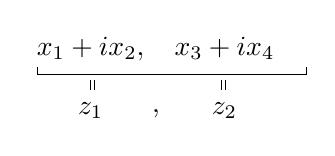
\begin{tikzpicture}[x=1cm,y=1cm]
\node at (.68,.30) {\(x_1+i x_2,\)};
\node at (2.38,.30) {\(x_3+i x_4\)};
\draw (0,.07)--(0,-.03)--(3.42,-.03)--(3.42,.07);
\draw (.68,-.10)--(.68,-.22) (.73,-.10)--(.73,-.22);
\draw (2.34,-.10)--(2.34,-.22) (2.39,-.10)--(2.39,-.22);
\node at (.68,-.48) {\(z_1\)};
\node at (1.51,-.52) {,};
\node at (2.38,-.48) {\(z_2\)};
\end{tikzpicture}}\endgroup\par}
\end{GelfandAdjacentEvidence}
\begin{GelfandAdjacentEvidence}{GELFAND-P000732}{4}


\(B_j(\lambda)\) выписывают сами как опер. ковар. дифф.
\[
(9)\quad \widehat B_1(\lambda)=\lambda\nabla_1+\overline{\nabla}_2,\qquad
\widehat B_2(\lambda)=\lambda\nabla_2+\overline{\nabla}_1.
\]
\Unclear{GELFAND-P000732}{lax-sign}{В обоих операторах (9) перед сопряжённой производной написан \(+\).}
\end{GelfandAdjacentEvidence}
\begin{GelfandAdjacentEvidence}{GELFAND-P000732}{5}

\[
(10)\quad
\nabla_1=A_1+iA_2+\frac{\partial}{\partial z_1},\qquad
\nabla_2=A_3+iA_4+\frac{\partial}{\partial z_2}.
\]
Связность \(=\{A_1,A_2,A_3,A_4\}\).

Мн-во компл. структур в \(\mathbb R^4\) (линейных) нумеруется одним компл. пар. \(\lambda\).
(На самом деле \(\lambda\) пробег. все компл. структуры).
\Unclear{GELFAND-P000732}{complex-structures}{В скобках написано «все компл. структуры». Других ограничений здесь не указано.}
\end{GelfandAdjacentEvidence}



\Needspace{7\baselineskip}
\begin{GelfandAdjacentEvidence}{GELFAND-P000733}{1}
\SourcePage{GELFAND-P000733}{unlabelled}
\uwave{Атья.}

(подход, сд. больше)
\SourceFigure{GELFAND-P000733}{top-arrow}{%
\par\begingroup\color{black}\GelfandFitDiagram{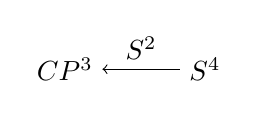
\begin{tikzpicture}[x=1cm,y=1cm]
\node (c) at (0,0) {\(\mathbb C P^3\)};
\node (s) at (1.78,0) {\(S^4\)};
\draw[<-] (c)-- node[above] {\(S^2\)} (s);
\end{tikzpicture}}\endgroup\par
В верхней записи стрелка направлена влево.}
\end{GelfandAdjacentEvidence}
\begin{GelfandAdjacentEvidence}{GELFAND-P000733}{2}

(рассл. Хопфа)

\SourceFigure{GELFAND-P000733}{hopf-composition}{%
\par\begingroup\color{black}\GelfandFitDiagram{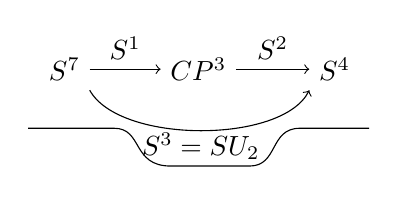
\begin{tikzpicture}[x=1cm,y=1cm]
\node (a) at (0,0) {\(S^7\)};
\node (b) at (1.7,0) {\(\mathbb C P^3\)};
\node (c) at (3.43,0) {\(S^4\)};
\draw[->] (a)--node[above]{\(S^1\)}(b);
\draw[->] (b)--node[above]{\(S^2\)}(c);
\draw[->] (a.south east) .. controls (.7,-.95) and (2.77,-.95) .. (c.south west);
\node at (1.73,-.98) {\(S^3=SU_2\)};
\draw (-.46,-.75)--(.63,-.75) .. controls (1,-.75) and (.85,-1.23) .. (1.35,-1.23)
 --(2.35,-1.23) .. controls (2.72,-1.23) and (2.6,-.75) .. (2.99,-.75)--(3.87,-.75);
\end{tikzpicture}}\endgroup\par}
\end{GelfandAdjacentEvidence}
\begin{GelfandAdjacentEvidence}{GELFAND-P000733}{3}


Важно:
\Unclear{GELFAND-P000733}{fibration-heading}{Заголовок предположительно читается «Важно».}
\end{GelfandAdjacentEvidence}
\begin{GelfandAdjacentEvidence}{GELFAND-P000733}{4}

\SourceFigure{GELFAND-P000733}{quaternion-fibration}{%
\par\begingroup\color{black}\GelfandFitDiagram{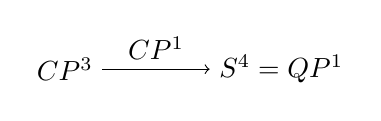
\begin{tikzpicture}[x=1cm,y=1cm]
\node (c) at (0,0) {\(\mathbb C P^3\)};
\node (s) at (2.75,0) {\(S^4=\mathbb Q P^1\)};
\draw[->] (c)--node[above]{\(\mathbb C P^1\)}(s);
\end{tikzpicture}}\endgroup\par}
\end{GelfandAdjacentEvidence}
\begin{GelfandAdjacentEvidence}{GELFAND-P000733}{5}


\(q_1,q_2\) --- кватернионы.
\[
q_1=(z_1,z_2),\qquad q_2=(z_3,z_4).
\]
\[
\vec z=e^{i\varphi}\vec z,\qquad
\vec q\to e^{ik}\vec q,\qquad |e^{ik}|=1.
\]
\Unclear{GELFAND-P000733}{complex-action-equality}{Между \(\vec z\) и экспонентой написано равенство.}
\end{GelfandAdjacentEvidence}
\begin{GelfandAdjacentEvidence}{GELFAND-P000733}{6}

\Unclear{GELFAND-P000733}{quaternion-exponent}{После \(i\) в показателе предположительно \(k\); знак похож также на \(\kappa\).}
\end{GelfandAdjacentEvidence}
\begin{GelfandAdjacentEvidence}{GELFAND-P000733}{7}


(ед. кватернион; они обр. гр. \(SU_2\)).
\[
\left(\underset{\text{кватерн.}}{\underline{z_1,z_2}}\ \middle|\
\underset{\text{кватерн.}}{\underline{z_3,z_4}}\right).
\]
Связн. \(A\) на \(S^4\) поднимем до [зачёркнуто: рассл.?]
[сверху вписано и обведено: связн.] [снизу вписано и обведено: \(\widetilde A\)] на \(\mathbb C P^3\).
\Unclear{GELFAND-P000733}{connection-cancellation}{Зачёркнутое слово предположительно «рассл.». Вставки обведены.}
\end{GelfandAdjacentEvidence}
\begin{GelfandAdjacentEvidence}{GELFAND-P000733}{8}


Связность с гр. \(SU_2\).
\[
SU_2=G
\]
\Unclear{GELFAND-P000733}{group-relation}{Знак перед \(G\) предположительно \(=\); нижняя черта густо обведена.}
\end{GelfandAdjacentEvidence}
\begin{GelfandAdjacentEvidence}{GELFAND-P000733}{9}


Связность порожд. квазикомплексную структуру.

(слои компл., а в гориз. пр-вах поднят. с базы).

\uwave{Слой \(\mathbb C^2\).}

Интегрируемость квазикомпл. структ. \(\Longleftrightarrow\) ур-я дуальности.

\(\Longleftrightarrow\) опер. \(\dfrac{\partial}{\partial z}\) коммутативны.
(предст. в виде коммут. пары)

\uwave{Повторение.}
\SourceFigure{GELFAND-P000733}{repeated-fibration}{%
\par\begingroup\color{black}\GelfandFitDiagram{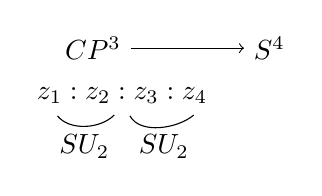
\begin{tikzpicture}[x=1cm,y=1cm]
\node (c) at (.48,0) {\(\mathbb C P^3\)};
\node (s) at (2.72,0) {\(S^4\)};
\draw[->] (c)--(s);
\node at (.85,-.6) {\(z_1:z_2:z_3:z_4\)};
\draw (.03,-.86) .. controls (.18,-1.05) and (.57,-1.03) .. (.75,-.85);
\draw (.95,-.86) .. controls (1.08,-1.10) and (1.56,-1.02) .. (1.76,-.85);
\node at (.37,-1.25) {\(SU_2\)};
\node at (1.38,-1.25) {\(SU_2\)};
\end{tikzpicture}}\endgroup\par}
\end{GelfandAdjacentEvidence}
\begin{GelfandAdjacentEvidence}{GELFAND-P000733}{10}

действуем здесь и там одними и теми же преобр. из \(SU_2\).

[зачёркнуто: \(SU_2\ldots\mathbb C P^3\)?]
\Unclear{GELFAND-P000733}{bottom-cancellation}{В зачёркнутой записи предположительно \(SU_2\) и \(\mathbb C P^3\). Знак между ними не установлен.}
\end{GelfandAdjacentEvidence}


\[
\text{Слой}=SU_2/(\text{диаг. матр.})=\mathbb C P^1.
\]
Есть компл. структура в базе и в слое.

Пусть на \(M^{2n}\) есть квазикомпл. структура

(способ превр. \(\forall\) кас. пр-во в комплексное)
\[
\begin{gathered}
\partial_1,\ldots,\partial_n\text{ --- базис векторов в кас. пр-ве}\\
\partial_{n+1},\ldots,\partial_{2n}
\end{gathered}
\]


\Needspace{7\baselineskip}
\begin{GelfandAdjacentEvidence}{GELFAND-P000734}{1}
\SourcePage{GELFAND-P000734}{71}
Пусть \(\nabla_j=\partial_j+i\partial_{n+j}\)
\[
\frac{\partial}{\partial y_\mu}\equiv i\frac{\partial}{\partial x_\mu}
\]
\Unclear{GELFAND-P000734}{coordinate-relation}{В рукописи между производными стоит знак из трёх черт \(\equiv\).}
\end{GelfandAdjacentEvidence}
\begin{GelfandAdjacentEvidence}{GELFAND-P000734}{2}

Треб., чтобы они \uwave{коммутировали}.

Это и есть интегрир. квазикомпл. структуры.
\Unclear{GELFAND-P000734}{integrability-overwrite}{В сокращении «квазикомпл.» средние буквы обведены густо.}
\end{GelfandAdjacentEvidence}



\Needspace{7\baselineskip}
\begin{GelfandAdjacentEvidence}{GELFAND-P000735}{1}
\SourcePage{GELFAND-P000735}{unlabelled}
\noindent\underline{15/XI-77.}\hspace{2em}\underline{Сем. Гельфанда.}

\underline{Б. С. Надь.}

Ряд зад. опер. прив. к постр. сжат. опер. на пр-вах \uwave{Харди}.
\Unclear{GELFAND-P000735}{opening-first-word}{Первое слово бледное, предположительно «Ряд».}
\end{GelfandAdjacentEvidence}
\begin{GelfandAdjacentEvidence}{GELFAND-P000735}{2}

\Unclear{GELFAND-P000735}{opening-second-word}{Второе слово читается предположительно как «зад.».}
\end{GelfandAdjacentEvidence}
\begin{GelfandAdjacentEvidence}{GELFAND-P000735}{3}

\Unclear{GELFAND-P000735}{opening-compressed}{Сокращение после «постр.» читается предположительно как «сжат.».}
\end{GelfandAdjacentEvidence}
\begin{GelfandAdjacentEvidence}{GELFAND-P000735}{4}


\(H^\infty\) --- огр. аналит. ф-и в круге.

[Зачёркнуто] \uwave{inner function}
\[
\underset{\mathrm{def}}{=}\quad |u\cdot e^{it}|=1
\]
\hspace*{2em} almost everywhere
\Unclear{GELFAND-P000735}{cancel-before-inner}{Зачёркнутые знаки перед «inner function» неразборчивы.}
\end{GelfandAdjacentEvidence}
\begin{GelfandAdjacentEvidence}{GELFAND-P000735}{5}

\Unclear{GELFAND-P000735}{boundary-product}{Между \(u\) и \(e^{it}\) в рукописи стоит точка.}
\end{GelfandAdjacentEvidence}
\begin{GelfandAdjacentEvidence}{GELFAND-P000735}{6}


\[
\bigwedge_\alpha u_\alpha
\]
--- наиб. внутр. делитель набора ф-й

\Unclear{GELFAND-P000735}{margin-right-curve}{На правом поле короткий изогнутый штрих. Его назначение неясно.}
\end{GelfandAdjacentEvidence}
\begin{GelfandAdjacentEvidence}{GELFAND-P000735}{7}

Blaschke decompos.:
\[
\forall\quad\text{[Зачёркнуто]}\quad u=u_i u_o
\]
\hspace*{2em} (теор. Смирнова)
\Unclear{GELFAND-P000735}{cancel-before-factorization}{Зачёркнутые знаки между \(\forall\) и \(u\) неразборчивы.}
\end{GelfandAdjacentEvidence}
\begin{GelfandAdjacentEvidence}{GELFAND-P000735}{8}

\Unclear{GELFAND-P000735}{outer-factor-subscript}{Последний нижний индекс предположительно \(o\).}
\end{GelfandAdjacentEvidence}
\begin{GelfandAdjacentEvidence}{GELFAND-P000735}{9}


\SourceFigure{GELFAND-P000735}{blaschke-diagram}{%
\par\begingroup\color{black}\GelfandFitDiagram{\begin{tikzpicture}[x=1cm,y=1cm]
\node at (0,0) {\(u_i=\)};
\node (b) at (1.05,0) {\(B\)};
\node at (1.56,0) {\(\cdot\)};
\node (s) at (2.02,0) {\(s\)};
\node (bl) at (.32,-1) [align=center] {произв.\\Блашке};
\node (sl) at (3.10,-.70) {singular};
\draw[->] (bl.north east) -- (b.south);
\draw[->] (sl.north west) -- (s.south east);
\end{tikzpicture}}\endgroup\par}
\end{GelfandAdjacentEvidence}
\begin{GelfandAdjacentEvidence}{GELFAND-P000735}{10}


ф-й с общим нулём и по мас. [Зачёркнуто].
\Unclear{GELFAND-P000735}{bottom-abbreviation}{Последнее сокращение предположительно «мас.».}
\end{GelfandAdjacentEvidence}
\begin{GelfandAdjacentEvidence}{GELFAND-P000735}{11}

\Unclear{GELFAND-P000735}{bottom-cancelled-group}{Зачёркнутая группа в конце строки неразборчива.}
\end{GelfandAdjacentEvidence}



\Needspace{7\baselineskip}
\begin{GelfandAdjacentEvidence}{GELFAND-P000736}{1}
\SourcePage{GELFAND-P000736}{unlabelled}
\SourceFigure{GELFAND-P000736}{singular-measure}{%
\par\begingroup\color{black}\GelfandFitDiagram{\begin{tikzpicture}[x=1cm,y=1cm]
\node at (0,0) {\(\displaystyle s(\lambda)=\exp\int_0^{2\pi}\frac{e^{it}+\lambda}{e^{it}-\lambda}\)};
\node (measure) at (2.67,0) {\(d\mu(t)\)};
\node (label) at (2.67,-.95) {синг. мера};
\draw[->] (label.north)--(measure.south);
\end{tikzpicture}}\endgroup\par}
\end{GelfandAdjacentEvidence}
\begin{GelfandAdjacentEvidence}{GELFAND-P000736}{2}

\Unclear{GELFAND-P000736}{initial-s-case}{Начальный знак предположительно \(s\), регистр не вполне ясен.}
\end{GelfandAdjacentEvidence}
\begin{GelfandAdjacentEvidence}{GELFAND-P000736}{3}


\SourceFigure{GELFAND-P000736}{divisor-labels}{%
\par\begingroup\color{black}\GelfandFitDiagram{\begin{tikzpicture}[x=1cm,y=1cm]
\node at (0,0) {\(\displaystyle\bigwedge_\alpha u_\alpha=\)};
\node (b) at (1.46,0) {\(B\)};
\node at (2.23,0) {\(\cdot\)};
\node (s) at (3.08,0) {\(S\)};
\node (zeros) at (1.35,-1.15) [align=center] {произв. по\\всем нулям};
\node[anchor=west] (lower) at ([xshift=1.5mm]zeros.east) [align=center] {соотв. нижней\\грани всех мер \(\mu_i\)};
\draw (b.south)--++(-.05,-.37);
\draw[->] (s.south)--(3.08,-.77);
\end{tikzpicture}}\endgroup\par}
\end{GelfandAdjacentEvidence}
\begin{GelfandAdjacentEvidence}{GELFAND-P000736}{4}

\Unclear{GELFAND-P000736}{factor-s-case}{Второй множитель предположительно прописное \(S\).}
\end{GelfandAdjacentEvidence}
\begin{GelfandAdjacentEvidence}{GELFAND-P000736}{5}


В алг. Харди неверно, что
\[
u\wedge v=xu+yv.
\]
Неверно, что даже

\SourceFigure{GELFAND-P000736}{outer-arrows}{%
\par\begingroup\color{black}\GelfandFitDiagram{\begin{tikzpicture}[x=1cm,y=1cm]
\node (h) at (0,0) {\(h\)};
\node at (1.14,0) {\((u\wedge v)=\)};
\node (ink) at (2.35,0) {\(\square\)};
\node at (3.56,0) {\((xu+yv)\)};
\node (outer) at (2.1,-.94) {внешняя};
\node[anchor=west] at ([xshift=1.1mm]outer.east) {(не им. внутр. делит.)};
\draw[->] (outer.west) to[out=180,in=290] (h.south east);
\draw[->,densely dashed] (outer.north) -- (ink.south);
\end{tikzpicture}}\endgroup\par}
\end{GelfandAdjacentEvidence}
\begin{GelfandAdjacentEvidence}{GELFAND-P000736}{6}

\Unclear{GELFAND-P000736}{overwritten-coefficient}{Знак перед скобками закрашен. Нижний штрих под ним также густо зачёркнут.}
\end{GelfandAdjacentEvidence}
\begin{GelfandAdjacentEvidence}{GELFAND-P000736}{7}

\Unclear{GELFAND-P000736}{margin-right-curve}{На правом поле прерывистый изогнутый штрих. Его назначение неясно.}
\end{GelfandAdjacentEvidence}
\begin{GelfandAdjacentEvidence}{GELFAND-P000736}{8}


\uwave{Фиксируем внутр. ф-ю \(\omega\).} Тогда \(\forall u,v\ \exists x,y\colon\)
\[
xu+yv=h_\omega(u\wedge v),\quad\text{где }h_\omega\wedge\omega=1
\]
(но \(h_\omega\) не обяз. внешний)
\Unclear{GELFAND-P000736}{outer-word}{Последнее слово предположительно «внешний». Средние буквы обведены густо.}
\end{GelfandAdjacentEvidence}
\begin{GelfandAdjacentEvidence}{GELFAND-P000736}{9}


На самом деле, можно выб. \(x,y=\mathrm{const}\)
\[
\text{\uwave{\(u+tv=h_t(u\wedge v)\)}}
\]
\uwave{M. Sherman} (красивые док-ва леммы)

\uwave{Обобщение:}

[зачёркнуто] \(\forall u_1,\ldots,u_r,\)
\Incomplete{GELFAND-P000736}{abandoned-before-quantifier}{Перед квантором переписанная группа неразборчива.}
\end{GelfandAdjacentEvidence}
\begin{GelfandAdjacentEvidence}{GELFAND-P000736}{10}

\[
u_1+tu_2+\cdots+t^{r-1}u_{r+1}
=h_t\Bigl(\bigwedge_k u_k\Bigr);\quad h_t\wedge\omega=1
\]
\Unclear{GELFAND-P000736}{sequence-final-index}{Последний нижний индекс предположительно \(r+1\).}
\end{GelfandAdjacentEvidence}
\begin{GelfandAdjacentEvidence}{GELFAND-P000736}{11}

\Incomplete{GELFAND-P000736}{sequence-index-underink}{Прежние штрихи под густой чертой в индексе неразборчивы.}
\end{GelfandAdjacentEvidence}
\begin{GelfandAdjacentEvidence}{GELFAND-P000736}{12}

(Кроме счётного мн-ва знач. \(t\))

и то же, для конечн. числа строчек

Дальше какие-то элем. преобр. матриц.

\underline{\underline{И. Кричевер.}}

\uwave{Рац. решения ур-я Кадомцева-Петвиашвили:}
\begin{equation*}
\tag*{(1)\hfill}
\frac34 u_{yy}+\frac{\partial}{\partial x}
\left\{\text{[зачёркнуто]}\frac{\partial u}{\partial t}
+\frac14(6uu_x+u_{xxx})\right\}=0
\end{equation*}
\Incomplete{GELFAND-P000736}{kp-cancel-before-time-derivative}{Зачёркнутый знак перед производной по времени неразборчив.}
\end{GelfandAdjacentEvidence}



\Needspace{7\baselineskip}
\begin{GelfandAdjacentEvidence}{GELFAND-P000737}{1}
\SourcePage{GELFAND-P000737}{78}
\underline{Теорема.} \uwave{Ищем рац. по \(x\) решения} \(u(x,y,t)\),
\uwave{убывающие при \(\lvert x\rvert\to\infty\).}
\uwave{Тогда} легко видеть, что
\Unclear{GELFAND-P000737}{easy-final-word}{Слово перед «видеть» читается как «легко». Последняя буква обведена густо.}
\end{GelfandAdjacentEvidence}
\begin{GelfandAdjacentEvidence}{GELFAND-P000737}{2}

\Incomplete{GELFAND-P000737}{easy-word-underink}{Прежние штрихи последней буквы под густой правкой неразборчивы.}
\end{GelfandAdjacentEvidence}
\begin{GelfandAdjacentEvidence}{GELFAND-P000737}{3}

\[
u(x,y,t)=\sum\frac{-2}{\bigl(x-x_j(y,t)\bigr)^2}
\]
\Unclear{GELFAND-P000737}{pole-argument-y}{Первый аргумент в \(x_j\) читается как \(y\) по нижней петле.}
\end{GelfandAdjacentEvidence}
\begin{GelfandAdjacentEvidence}{GELFAND-P000737}{4}

\Incomplete{GELFAND-P000737}{pole-argument-underink}{Прежние штрихи аргумента под правкой неразборчивы.}
\end{GelfandAdjacentEvidence}
\begin{GelfandAdjacentEvidence}{GELFAND-P000737}{5}


1) \uwave{Полюса по \(y\) движутся в соотв. с сист. Мозера} \uwave{с гамильтонианом}
\[
H=\frac12\sum p_j^2+\sum_{i<j}\frac{1}{(x_i-x_j)^2}
\]
(\(t\) \uwave{фиксировано})

2) \uwave{Полюса по \(t\) двиг.} [зачёркнуто] \uwave{по гамильтониану \(F_3\), явл. одним из интегралов сист. Мозера}
\Incomplete{GELFAND-P000737}{cancel-after-time-motion}{Зачёркнутый знак после «двиг.» неразборчив.}
\end{GelfandAdjacentEvidence}
\begin{GelfandAdjacentEvidence}{GELFAND-P000737}{6}


Получ. 2 коммутирующих потока, опред. [вписано сверху: (рац.)] реш. ур-я (1).

\SourceFigure{GELFAND-P000737}{separator}{%
\par\begingroup\color{black}\GelfandFitDiagram{\begin{tikzpicture}[x=1cm,y=1cm]
\draw (0,0)--(1.15,0);
\fill (1.49,-.01) circle[radius=.022];
\draw (2.21,-.01)--(3.64,-.06);
\end{tikzpicture}}\endgroup\par}
\end{GelfandAdjacentEvidence}
\begin{GelfandAdjacentEvidence}{GELFAND-P000737}{7}


\[
(1)\Longleftrightarrow
\left[\frac{\partial}{\partial y}-L_1,\frac{\partial}{\partial t}-L_2\right]=0,
\]
\[
L_1=\frac{d^2}{dx^2}+u,\qquad
L_2=\frac{d^3}{dx^3}+\frac32u\frac{d}{dx}+u
\]
\Incomplete{GELFAND-P000737}{l2-coefficient-underink}{Коэффициент читается как \(3/2\). Прежние штрихи под густой правкой неразборчивы.}
\end{GelfandAdjacentEvidence}
\begin{GelfandAdjacentEvidence}{GELFAND-P000737}{8}

\Unclear{GELFAND-P000737}{l2-final-term}{Последнее слагаемое записано как \(+u\).}
\end{GelfandAdjacentEvidence}
\begin{GelfandAdjacentEvidence}{GELFAND-P000737}{9}


Получ. коммутативные подалгебры в \(\mathcal D_n\) (тело частных кольца дифф. опер. с полин. коэфф. от \(n\) перем.)

След. раз \underline{Ю. И. Манин}
\Unclear{GELFAND-P000737}{bibliography-abbreviation}{Бледкое сокращение перед «раз» читается предположительно как «След.».}
\end{GelfandAdjacentEvidence}



\clearpage\pdfbookmark[0]{Глава 12}{gelfand-archive-chapter-12}
\section*{Глава 12}


\Needspace{7\baselineskip}
\begin{GelfandAdjacentEvidence}{GELFAND-P000738}{1}
\SourcePage{GELFAND-P000738}{6}
\noindent\underline{\underline{21/\(\overline{\underline{\mathrm{XI}}}\)-77.}}\qquad
\underline{\underline{Сем. Гельфанда.}}

\SourceFigure{GELFAND-P000738}{speaker-box}{%
\par{\setlength{\fboxsep}{3pt}\fcolorbox{red}{white}{\underline{\textbf{Ю. И. Манин.}}}}\par}
\end{GelfandAdjacentEvidence}
\begin{GelfandAdjacentEvidence}{GELFAND-P000738}{2}


(о работе с \uwave{В. Дринфельдом})

\underline{Описание автодуальных решений ур-й Янга-Миллса.}

\(\mathbb R^4\ni(x_1,x_2,x_3,x_4)\). \qquad Неизвестные функции:

\[
A_\mu(x)\in u(r),\qquad r\geq 2
\]
(эрмитовы или антиэрмитовы матрицы; в алгебре Ли)
\SourceFigure{GELFAND-P000738}{algebra-pointer}{%
\par\begingroup\color{black}\GelfandFitDiagram{\begin{tikzpicture}[x=1cm,y=1cm]
\node (algebra) at (0,0) {\(u(r)\)};
\draw (-.48,-.22)--(-.48,-.34)--(.46,-.34)--(.46,-.22);
\node (label) at (1.95,-.83) [align=left] {алгебра Ли \(U(r)\)};
\draw[->] (label.north west)--(.17,-.39);
\end{tikzpicture}}\endgroup\par}
\end{GelfandAdjacentEvidence}
\begin{GelfandAdjacentEvidence}{GELFAND-P000738}{3}

\(u(r)\) --- множество косоэрмитовых \(r\times r\) матриц.

\begin{equation*}
\tag*{(1)\hfill}
F_{\mu\nu}(x)\underset{\mathrm{def}}{=}
\frac{\partial}{\partial x_\mu}A_\nu
-\frac{\partial}{\partial x_\nu}A_\mu+[A_\mu,A_\nu]
\end{equation*}

1) \uwave{Уравнения дуальности:}

\(\rho\sigma\) --- доп. пара индексов к \(\mu\nu\), \quad \(F_{\mu\nu}=\pm F_{\rho\sigma}\); точнее:
\begin{equation*}
\tag*{(2)\hfill}
F_{\mu\nu}=\varepsilon^{\mu\nu\rho\sigma}F_{\rho\sigma}
\end{equation*}
(\(\varepsilon^{\mu\nu\rho\sigma}\) --- знак перестановки).

2) \uwave{Условия регулярности:} \quad А) в конечн. точках \quad Б) в бесконечности

А) особенности могут быть в конечных точках сняты калибровкой.

Точнее, рассм. расслоение \(\mathbb C^r\times\mathbb R^4\) и в нем базис сечений;
ковариантн. диффер., определяемое матрицами \(A_\mu\), задаётся формулой:
\begin{equation*}
\tag*{(3)\hfill}
\partial_\mu\begin{pmatrix}s_1\\ \vdots\\ s_r\end{pmatrix}
=A_\mu\begin{pmatrix}s_1\\ \vdots\\ s_r\end{pmatrix},
\qquad
\partial_\mu s_i=\sum_{i=1}^{r}A_\mu^{ij}s_j.
\end{equation*}
\Unclear{GELFAND-P000738}{eq-03-summation}{Нижний предел суммы написан \(i=1\). Индекс \(i\) у \(s_i\) слева обведён густо.}
\end{GelfandAdjacentEvidence}
\begin{GelfandAdjacentEvidence}{GELFAND-P000738}{4}

\SourceFigure{GELFAND-P000738}{section-pointer}{%
\par\begingroup\color{black}\GelfandFitDiagram{\begin{tikzpicture}[x=1cm,y=1cm]
\node at (0,0) {\(\partial_\mu\)};
\node (sections) at (.82,0) {\(\begin{pmatrix}s_1\\ \vdots\\ s_r\end{pmatrix}\)};
\node (basis) at (2.69,-1.22) [align=left] {базисные сечения\\ \(s_1,\ldots,s_r\)};
\draw[->] (basis.north west)--(sections.south);
\end{tikzpicture}}\endgroup\par}
\end{GelfandAdjacentEvidence}
\begin{GelfandAdjacentEvidence}{GELFAND-P000738}{5}


Перейдём к другому базису. Получим преобразование (калибровочное преобразование).
\begin{equation*}
\tag*{(4)\hfill}
A_\mu\mapsto u^{-1}\partial_\mu u+u^{-1}A_\mu u=A'_\mu
\end{equation*}

\uwave{Условие регулярности в конечной точке:} имеется настоящая связность без особенностей, т. е. особ. \(A_\mu\) можно ликвидировать калибровкой.

Переход:
\SourceFigure{GELFAND-P000738}{basis-change}{%
\par\begingroup\color{black}\GelfandFitDiagram{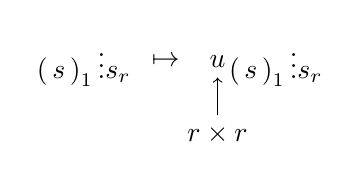
\begin{tikzpicture}[x=1cm,y=1cm]
\node at (0,0) {\(\begin{pmatrix}s_1\\ \vdots\\ s_r\end{pmatrix}\)};
\node at (1.04,0) {\(\mapsto\)};
\node (change) at (1.70,0) {\(u\)};
\node at (2.44,0) {\(\begin{pmatrix}s_1\\ \vdots\\ s_r\end{pmatrix}\)};
\node (size) at (1.70,-.92) {\(r\times r\)};
\draw[->] (size.north)--(change.south);
\end{tikzpicture}}\endgroup\par}
\end{GelfandAdjacentEvidence}
\begin{GelfandAdjacentEvidence}{GELFAND-P000738}{6}


Б) \uwave{Условия в} \(P=\infty\).

Расслоение на
\(\mathbb R^4\) продолжается до рассл. над \(S^4=\mathbb R^4\cup\{\infty\}\).
\SourceFigure{GELFAND-P000738}{bundle-projection}{%
\par\begingroup\color{black}\GelfandFitDiagram{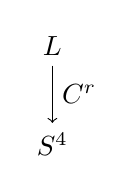
\begin{tikzpicture}[x=1cm,y=1cm]
\node (bundle) at (0,0) {\(L\)};
\node (sphere) at (0,-1.24) {\(S^4\)};
\draw[->] (bundle)--node[right]{\(\mathbb C^r\)}(sphere);
\end{tikzpicture}}\endgroup\par}
\end{GelfandAdjacentEvidence}

\(L\) --- пр-во нашего расслоения.

\uwave{Усл. регулярности:} Связность \(\partial_\mu\) продолжается до связности в \(L\) над \(S^4\)
(расслоение \(L\) уже не обязательно тривиально)


\Needspace{7\baselineskip}
\begin{GelfandAdjacentEvidence}{GELFAND-P000739}{1}
\SourcePage{GELFAND-P000739}{unlabelled}
Это тоже означает, что на бесконечности подкруткой можно ликвидировать особенность.

Существенный инвариант решения --- расслоение \(L\). Это дискретный инвариант. На \(L\) структура унитарного расслоения.

\uwave{Классификация} \(L\).

Склейка тривиализаций на экваторе даёт отображение \(S^3\to U(r)\), т. е. элемент \(\pi_3(U(r))=\mathbb Z\).

(\(SU(2)\subset U(r)\), \(SU(2)\cong S^3\); отсюда целочисленный достаточный инвариант
\(=\) степень отображения \(n\) \(=\) число Понтрягина)
\Unclear{GELFAND-P000739}{integer-invariant}{Слово после «целочисленный» читается как «достаточный». Первые буквы обведены густо.}
\end{GelfandAdjacentEvidence}
\begin{GelfandAdjacentEvidence}{GELFAND-P000739}{2}


вложение \(SU(2)\subset U(r)\) берётся вида
\SourceFigure{GELFAND-P000739}{block-embedding}{%
\par\begingroup\color{black}\GelfandFitDiagram{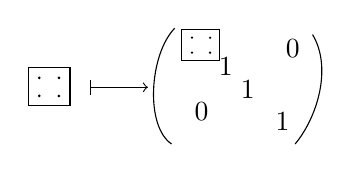
\begin{tikzpicture}[x=1cm,y=1cm]
\draw (0,0) rectangle (.53,.48);
\foreach \x in {.14,.39} \foreach \y in {.12,.35} {\fill (\x,\y) circle[radius=.019];}
\draw[|->] (.78,.23)--(1.52,.23);
\draw (1.86,.98) .. controls (1.54,.65) and (1.48,-.26) .. (1.82,-.49);
\draw (3.61,.90) .. controls (3.86,.49) and (3.68,-.14) .. (3.39,-.49);
\draw (1.95,.57) rectangle (2.43,.96);
\foreach \x in {2.08,2.31} \foreach \y in {.67,.86} {\fill (\x,\y) circle[radius=.016];}
\node at (2.51,.49) {\(1\)};
\node at (2.79,.20) {\(1\)};
\node at (3.23,-.20) {\(1\)};
\node at (3.36,.72) {\(0\)};
\node at (2.20,-.08) {\(0\)};
\end{tikzpicture}}\endgroup\par}
\end{GelfandAdjacentEvidence}
\begin{GelfandAdjacentEvidence}{GELFAND-P000739}{3}


\uwave{Будем считать} \(n\geq0\) и дуальные условия

(\(n<0\ \Rightarrow\) можно изменить знак в ур-и (2))\\
\hspace*{2em}--- антидуальные реш. --- свести к \(n>0\))
\Unclear{GELFAND-P000739}{extra-parenthesis}{После «(2)» и в конце следующей строки видны закрывающие скобки.}
\end{GelfandAdjacentEvidence}
\begin{GelfandAdjacentEvidence}{GELFAND-P000739}{4}


\uwave{План дальнейшего:}

[Зачёркнутая строка]
\Incomplete{GELFAND-P000739}{plan-deleted-line}{Строка под заголовком густо зачёркнута и не читается.}
\end{GelfandAdjacentEvidence}
\begin{GelfandAdjacentEvidence}{GELFAND-P000739}{5}


\SourceFigure{GELFAND-P000739}{diagram-plan}{%
\par\begingroup\color{black}\GelfandFitDiagram{\begin{tikzpicture}[x=.82cm,y=.85cm,font=\small]
\node (start) at (0,0) {\(\left(\begin{gathered}L\\\downarrow\\S^4\end{gathered},\,A_\mu\right)\)};
\draw[->] plot[smooth] coordinates {(1.0,0) (1.15,.07) (1.29,-.045) (1.45,.07) (1.61,-.04) (1.79,.03) (2.08,.015)};
\draw (2.60,.54)--(2.40,.54)--(2.40,-2.57)--(2.60,-2.57);
\node (trivial) at (3.39,.47) {\(H\times S^4\)};
\node (base) at (3.40,-.61) {\(S^4\)};
\draw[->] (trivial.south)--(base.north);
\node (rank) at (3.88,1.32) {\(2n+r\)};
\draw[->] (rank.south west)--(trivial.north west);
\node at (6.39,.14) {\(H=\mathbb C^{2n+r}\),};
\node[anchor=west,align=left] at (2.53,-1.68) {Здесь:\\{[зачёркнуто]}\\эрмитова метрика\\тривиальная связность};
\draw[->] (1.99,-1.64)--(.82,-.66);
\node (orthogonal) at (.18,-3.55) [align=left] {Явно конструируемое\\разл. на ортог. части};
\draw[->] (orthogonal.north)--(1.19,-1.18);
\end{tikzpicture}}\endgroup\par}
\end{GelfandAdjacentEvidence}
\begin{GelfandAdjacentEvidence}{GELFAND-P000739}{6}

\Incomplete{GELFAND-P000739}{diagram-deleted-caption}{Внутри большой скобки зачёркнуто короткое словосочетание. Начальная буква похожа на «с».}
\end{GelfandAdjacentEvidence}
\begin{GelfandAdjacentEvidence}{GELFAND-P000739}{7}


\SourceFigure{GELFAND-P000739}{rank-decomposition}{%
\par\begingroup\color{black}\(\begin{array}{lccccc}
\text{Размерности:}&2n+r&&r&&2n\\
&\downarrow&&\downarrow&&\downarrow\\
\text{Разложение:}&H\times S^4&=&L&\oplus&L^\perp
\end{array}\)\endgroup\par}
\end{GelfandAdjacentEvidence}
\begin{GelfandAdjacentEvidence}{GELFAND-P000739}{8}


\(\{A_\mu\}\) --- прямое слагаемое тривиальной связности в \(H\times S^4\)

(Дифференцируем и проектируем на \(L\)).

Унитарность связности доказывается.

[Это обобщение того, что риманово пр-во можно вложить в евклидово; можно ли [вписано сверху: всегда] вложить расслоение со связностью?]
\Unclear{GELFAND-P000739}{riemannian-space}{После «риманово» написано сокращение «пр-во».}
\end{GelfandAdjacentEvidence}
\begin{GelfandAdjacentEvidence}{GELFAND-P000739}{9}


Какие разложения приводят к автодуальным полям?

Надо от базы \(S^4\) перейти к её \uwave{комплексификации}.

В \(\mathbb C^4\) рассмотрим отобр.
\[
\sigma:\ z\mapsto(-\overline z_2,\overline z_1,-\overline z_4,\overline z_3).
\]
\SourceFigure{GELFAND-P000739}{coordinate-pointer}{%
\par\begingroup\color{black}\GelfandFitDiagram{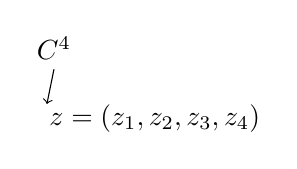
\begin{tikzpicture}[x=1cm,y=1cm]
\node (space) at (0,.89) {\(\mathbb C^4\)};
\node at (1.28,0) {\(z=(z_1,z_2,z_3,z_4)\)};
\draw[->] (space.south)--(-.09,.18);
\end{tikzpicture}}\endgroup\par}
\end{GelfandAdjacentEvidence}

(в кватернионах умножение на \(i\))

У \(\sigma\) нет неподв. точек (\(\text{кроме }0\)) и неподв. прямых, а есть инвар. плоскости
\begin{equation*}
\tag*{(5)\hfill}
\mathbb C z+\mathbb C\sigma(z)\subset\mathbb C^4
\end{equation*}


\Needspace{7\baselineskip}
\begin{GelfandAdjacentEvidence}{GELFAND-P000740}{1}
\SourcePage{GELFAND-P000740}{7}
Будем называть их \uwave{вещественными} (или \uwave{\(\sigma\)-инвариантными})
(\(\sigma\) --- инволюция).

\begin{equation*}
\tag*{(6)\hfill}
\{\sigma\text{-инвар. плоскости}\}=S^4
\end{equation*}
(\uwave{док-во опускается})

(в \(\mathbb C P^3\) это мн-во \(\sigma\)-инвар. прямых).

\(E^4\subset\) [зачёркнуто] \(S^4=E^4\cup\{\infty\}\).
\Incomplete{GELFAND-P000740}{compactification-cancel}{Между знаком включения и \(S^4\) густо зачёркнут знак.}
\end{GelfandAdjacentEvidence}
\begin{GelfandAdjacentEvidence}{GELFAND-P000740}{2}


Отсюда есть отображение
\begin{equation*}
\tag*{(7)\hfill}
\mathbb C^4\setminus\{0\}\overset{D}{\longrightarrow}S^4\supset E^4.
\end{equation*}
\[
z\longmapsto \sigma\text{-инвар. плоск., прох. через }z.
\]
Напишем \(D\) в координатах (\(\text{в } E^4\) координаты \((x_i)\)).
Нормировка как у Захарова-Белавина.

\[
(z_1,z_2,z_3,z_4)\longmapsto
\begin{cases}
x_2+i x_1=\dfrac{z_1\bar z_3+\bar z_2 z_4}{|z_3|^2+|z_4|^2},\\[6pt]
x_4+i x_3=\dfrac{\bar z_2 z_3-z_1\bar z_4}{|z_3|^2+|z_4|^2}.
\end{cases}
\]
(плюккеровы координаты [вписано сверху: \(\sigma\)-инв.] плоскости, проходящей через т. \(z\))
\Unclear{GELFAND-P000740}{plane-insertion}{Сокращение «\(\sigma\)-инв.» вписано над строкой с указанием места вставки.}
\end{GelfandAdjacentEvidence}
\begin{GelfandAdjacentEvidence}{GELFAND-P000740}{3}


Это отображение
\[
\mathbb C^4\setminus\{z_3=z_4=0\}\longrightarrow E^4.
\]
\underline{Замечание:} для восстан. \(\sigma\)-инв. пл. достаточно 3-х координат.

\underline{\underline{Лемма 1}}
\(\bigl(\overset{4}{\text{А}}\,
\overset{2}{\text{У}}\,
\overset{1?}{\text{Б}}\,
\overset{3}{\text{З}}\bigr.\)
--- Атья, Уорд, Белавин, Захаров).
\Unclear{GELFAND-P000740}{attribution-numeral}{Над «Б» густой вертикальный штрих, предположительно 1. Остальные цифры читаются 4, 2 и 3.}
\end{GelfandAdjacentEvidence}
\begin{GelfandAdjacentEvidence}{GELFAND-P000740}{4}

\Unclear{GELFAND-P000740}{belavin-correction}{Начало фамилии «Белавин» обведено густо.}
\end{GelfandAdjacentEvidence}
\begin{GelfandAdjacentEvidence}{GELFAND-P000740}{5}


а)
\[
D^*(dx_\mu\wedge dx_\nu+\varepsilon^{\mu\nu\rho\sigma}dx_\rho\wedge dx_\sigma)
\quad\text{--- форма типа }(1,1).
\]
(Рассмотрим такие формы; поднимем их на \(\mathbb C^4\setminus0\) с помощью \(D\))

б)
\[
\left[D^*\left(\begin{array}{l}
dx_1\wedge dx_2,\\
dx_1\wedge dx_3,\\
dx_1\wedge dx_4
\end{array}\right)\right]^{2,0}
\qquad\text{линейно независимы.}
\]
[зачёркнуто]
\Incomplete{GELFAND-P000740}{independence-cancel}{После «линейно независимы» густо зачёркнут короткий фрагмент.}
\end{GelfandAdjacentEvidence}
\begin{GelfandAdjacentEvidence}{GELFAND-P000740}{6}


\((2,0)\)-компоненты.

\underline{Следствие 1} (АУ).

\begin{equation*}
\tag*{(8)\hfill}
\left[D^*\left(\sum F_{\mu\nu}\,dx_\mu\wedge dx_\nu\right)\right]=0
\quad\Longleftrightarrow\quad
F_{\mu\nu}=\varepsilon^{\mu\nu\rho\sigma}F_{\rho\sigma}.
\end{equation*}
\Unclear{GELFAND-P000740}{corollary-projection}{У закрывающей квадратной скобки в (8) показатель компоненты не указан.}
\end{GelfandAdjacentEvidence}



\Needspace{7\baselineskip}
\begin{GelfandAdjacentEvidence}{GELFAND-P000741}{1}
\SourcePage{GELFAND-P000741}{unlabelled}
\underline{Следствие \(1'\)} (БЗ)

\SourceFigure{GELFAND-P000741}{derivative-annotations}{%
\par\begingroup\color{black}\GelfandFitDiagram{\begin{tikzpicture}[x=1cm,y=1cm]
\node at (-.70,0) {\((9)\)};
\node at (1.75,0) {\(\displaystyle\left[\frac{\partial}{\partial z_\mu},
  \frac{\partial}{\partial z_\nu}\right]=0\)};
\node (covariant) at (1.45,-1.49) [align=center] {ковариантные\\производные};
\draw[->] ([xshift=-5mm]covariant.north)--(1.02,-.57);
\draw[->] ([xshift=4mm]covariant.north)--(1.99,-.57);
\end{tikzpicture}}\endgroup\par}
\end{GelfandAdjacentEvidence}
\begin{GelfandAdjacentEvidence}{GELFAND-P000741}{2}

\Unclear{GELFAND-P000741}{covariant-ending}{Окончание слова «ковариантные» густо обведено.}
\end{GelfandAdjacentEvidence}
\begin{GelfandAdjacentEvidence}{GELFAND-P000741}{3}


\underline{\underline{Белавин.}} Или:
\begin{equation*}
\tag{10}
[\nabla_\mu,\nabla_\nu]=0,
\end{equation*}
где
\begin{equation*}
\tag{11}
\nabla_\mu=\frac{\partial}{\partial z_\mu}+C_\mu,
\end{equation*}
\begin{equation*}
\tag{12}
\left[D^*\left(\sum A_\mu\,dx_\mu\right)\right]^{1,0}=\sum C_a\,dz_a
\end{equation*}
\Unclear{GELFAND-P000741}{equation-number}{Цифра 2 в номере формулы (12) густо обведена.}
\end{GelfandAdjacentEvidence}
\begin{GelfandAdjacentEvidence}{GELFAND-P000741}{4}

\Unclear{GELFAND-P000741}{form-index}{Индексы в правой части (12) предположительно \(a\), возможно \(\alpha\).}
\end{GelfandAdjacentEvidence}
\begin{GelfandAdjacentEvidence}{GELFAND-P000741}{5}


Или: положим
\begin{equation*}
\tag{13}
C_i(z)=\frac{\partial x_\mu}{\partial z_i}A_\mu(x)
\end{equation*}
\Unclear{GELFAND-P000741}{coordinate-retraced}{Знак \(z\) в знаменателе (13) густо обведён.}
\end{GelfandAdjacentEvidence}
\begin{GelfandAdjacentEvidence}{GELFAND-P000741}{6}


Тогда
\begin{equation*}
\tag{14}
\text{[зачёркнуто]}\quad
\frac{\partial C_k}{\partial z_i}-\frac{\partial C_i}{\partial z_k}+[C_i,C_k]=0
\end{equation*}
\Incomplete{GELFAND-P000741}{equation14-cancel}{Первый знак зачёркнутой группы похож на \(\partial\). Остальные знаки неразборчивы.}
\end{GelfandAdjacentEvidence}
\begin{GelfandAdjacentEvidence}{GELFAND-P000741}{7}

в силу уравнений дуальности.

Или:
\begin{equation*}
\tag{15}
[L_1,L_2]=0,
\end{equation*}
где
\begin{equation*}
\tag{\(16'\)}
L_1=\lambda(\nabla_1-i\nabla_2)+(\nabla_3+i\nabla_4),
\end{equation*}
\Unclear{GELFAND-P000741}{lax-i-retraced}{Знак после минуса в (16′) обведён густо, предположительно \(i\).}
\end{GelfandAdjacentEvidence}
\begin{GelfandAdjacentEvidence}{GELFAND-P000741}{8}

\begin{equation*}
\tag{\(16''\)}
L_2=\lambda(\nabla_3-i\nabla_4)-(\nabla_1+i\nabla_2),
\end{equation*}
\Unclear{GELFAND-P000741}{lax-sign}{Между скобками в (16″) густая горизонтальная черта и короткие вертикальные следы. Читается предположительно как минус.}
\end{GelfandAdjacentEvidence}
\begin{GelfandAdjacentEvidence}{GELFAND-P000741}{9}

\begin{equation*}
\tag{17}
\nabla_\mu\equiv\partial_\mu+A_\mu
\end{equation*}

\underline{\underline{М.}} \underline{Конструкция расслоений.} Они будут конструироваться слева.
\SourceFigure{GELFAND-P000741}{bundle-diagram}{%
\par\begingroup\color{black}\GelfandFitDiagram{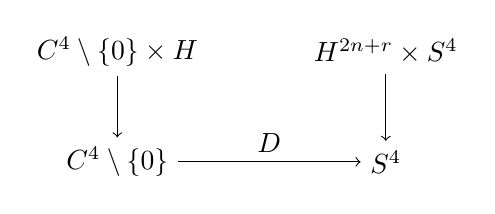
\begin{tikzpicture}[x=1cm,y=1cm]
\node (left) at (0,0) {\(\mathbb C^4\setminus\{0\}\times H\)};
\node (right) at (3.41,0) {\(H^{2n+r}\times S^4\)};
\node (leftbase) at (0,-1.40) {\(\mathbb C^4\setminus\{0\}\)};
\node (rightbase) at (3.41,-1.40) {\(S^4\)};
\draw[->] (left)--(leftbase);
\draw[->] (right)--(rightbase);
\draw[->] (leftbase)--node[above]{\(D\)}(rightbase);
\end{tikzpicture}}\endgroup\par}
\end{GelfandAdjacentEvidence}
\begin{GelfandAdjacentEvidence}{GELFAND-P000741}{10}


\uwave{Объекты линейной алгебры} \(\Rightarrow\) прямое слаг. в \(H\times S^4\).

\(H\) --- \((2n+r)\)-мерное эрмитово пространство,\\
\hspace*{2em}форма \(Q\).

Рассмотрим [зачёркнуто]
\begin{equation*}
\tag{18}
I\subset H\otimes_{\mathbb C}\mathbb C^4\qquad(*)
\end{equation*}
\Incomplete{GELFAND-P000741}{object-mark}{Перед (18) отдельно виден небольшой зачёркнутый знак.}
\end{GelfandAdjacentEvidence}
\begin{GelfandAdjacentEvidence}{GELFAND-P000741}{11}

\(I\) --- \(n\)-мерное подпространство

\SourceFigure{GELFAND-P000741}{object-bracket}{%
\par\begingroup\color{black}\GelfandFitDiagram{\begin{tikzpicture}[x=1cm,y=1cm]
\draw (0,.81)--(.16,.81)--(.16,-.81)--(0,-.81);
\node[anchor=west] at (.31,0) {\uwave{объект}};
\end{tikzpicture}}\endgroup\par
Правая скобка охватывает запись от определения \(H\) до строки о подпространстве \(I\).}
\end{GelfandAdjacentEvidence}



\Needspace{7\baselineskip}
\begin{GelfandAdjacentEvidence}{GELFAND-P000742}{1}
\SourcePage{GELFAND-P000742}{8}
\uwave{Условия.}

По объекту строим что-то вроде расслоения.

\(L(*)=\) «система линейных пр-в над \(S^4\)».

\SourceFigure{GELFAND-P000742}{plane-description}{%
\par\begingroup\color{black}\GelfandFitDiagram{\begin{tikzpicture}[x=1cm,y=1cm]
\node (vector) at (-.30,1.19) {\(z\in\mathbb C^4\)};
\node (plane) at (0,0) {\([z,\sigma(z)]\)};
\draw[->] (vector.south)--(-.45,.31);
\node[anchor=west] at (.79,0) {\(=\text{плоскость.}=\left\{\begin{array}{l}
\ell_1=0\\ \ell_2=0
\end{array}\right\}\)};
\end{tikzpicture}}\endgroup\par}
\end{GelfandAdjacentEvidence}
\begin{GelfandAdjacentEvidence}{GELFAND-P000742}{2}

\(\ell_{1,2}:\mathbb C^4\to\mathbb C\) --- линейные формы.

\SourceFigure{GELFAND-P000742}{image-diagram}{%
\par\begingroup\color{black}\GelfandFitDiagram{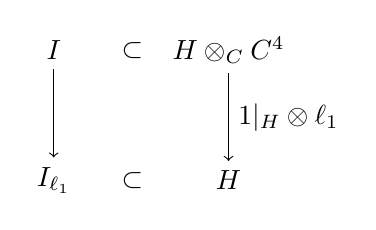
\begin{tikzpicture}[x=1cm,y=1cm]
\node (i) at (0,0) {\(I\)};
\node at (1,0) {\(\subset\)};
\node (tensor) at (2.22,0) {\(H\otimes_{\mathbb C}\mathbb C^4\)};
\node (image) at (0,-1.65) {\(I_{\ell_1}\)};
\node at (1,-1.65) {\(\subset\)};
\node (h) at (2.22,-1.65) {\(H\)};
\draw[->] (i)--(image);
\draw[->] (tensor)--node[right]{\(1|_H\otimes\ell_1\)}node[left]{\(\square\)}(h);
\end{tikzpicture}}\endgroup\par}
\end{GelfandAdjacentEvidence}
\begin{GelfandAdjacentEvidence}{GELFAND-P000742}{3}

\Incomplete{GELFAND-P000742}{image-diagram-mark}{Слева от правой стрелки густо обведённый знак неразборчив.}
\end{GelfandAdjacentEvidence}
\begin{GelfandAdjacentEvidence}{GELFAND-P000742}{4}

\Unclear{GELFAND-P000742}{identity-subscript}{Справа от стрелки написано \(1|_H\otimes\ell_1\).}
\end{GelfandAdjacentEvidence}
\begin{GelfandAdjacentEvidence}{GELFAND-P000742}{5}


Аналогично строится \(I_{\ell_2}\).

Итак, построено 2 подпр-ва \(I_{\ell_1},I_{\ell_2}\subset H\)

Оказывается, что
\[
I_{\ell_1}+I_{\ell_2}\quad \text{[зачёркнуто: зависит?]}
\]
\Unclear{GELFAND-P000742}{dependence-cancel}{Зачёркнутое слово справа от суммы предположительно «зависит».}
\end{GelfandAdjacentEvidence}
\begin{GelfandAdjacentEvidence}{GELFAND-P000742}{6}

зависит лишь от \(\sigma\)-инвар. плоскости \([z,\sigma(z)]\), т. е. точки \(S^4\)
\[
(I_{\ell_1}+I_{\ell_2})^\perp
=\text{лин. подпр-во в }H,\ \text{отвечающее }[z,\sigma(z)].
\]

\uwave{Условие 1.} Должно получиться расслоение
(размерности максимальны, т. е. правильны), а именно
\begin{equation*}
\tag{19}
\dim(I_{\ell_1}+I_{\ell_2})^\perp=r
\end{equation*}

\uwave{Условие} 2. Эрмитовость расслоения.

Форма \(Q|_{I_{\ell_1}+I_{\ell_2}}>0\)

(a priori \(Q\) не предполагается \(>0\), но оказывается, что при этом условии это так).

Получается прямое слагаемое. Связность получается проектированием тривиальной.

\underline{Теорема 1.} \uwave{Так получаются все} [вписано сверху: \uwave{автодуальные}]
\uwave{решения уравнения Я.-М.}, \uwave{неизом. рассл. отвечают неэквив. решения}.
\Unclear{GELFAND-P000742}{self-dual-insertion}{Слово «автодуальные» вписано над словом «решения» и подчёркнуто волнистой чертой.}
\end{GelfandAdjacentEvidence}


Пропущено ещё одно условие.

Ур-я берём:
\[
\left\{\begin{array}{l}
\ell(z)=0\\
\ell(\sigma z)=0
\end{array}\right\}
\]


\Needspace{7\baselineskip}
\begin{GelfandAdjacentEvidence}{GELFAND-P000743}{1}
\SourcePage{GELFAND-P000743}{unlabelled}
\underline{Условие} 0.

\begin{equation*}
\tag{20}
Q(I_\ell,I_{\ell\circ\sigma})=0
\end{equation*}
\uwave{т. е.} \(I_\ell\) и \(I_{\ell\circ\sigma}\) \uwave{ортогональны}.

Получилась задача линейной алгебры.

\underline{\underline{Г.}} она содержится в неопубл. работе Гельфанда и Пономарёва о четверках с автоморфизмом.

\underline{Пономарёв:}
\[
I\hookrightarrow H\oplus H\oplus H\oplus H\longrightarrow A\longrightarrow 0
\]
\Unclear{GELFAND-P000743}{sequence-inclusion}{У первого включения виден наконечник. Первый знак прямой суммы густо обведён.}
\end{GelfandAdjacentEvidence}
\begin{GelfandAdjacentEvidence}{GELFAND-P000743}{2}

Образы компонент \(H\) в \(A\) дают 4 подпр-ва.

Комплексные инварианты 4-ки описаны.

Эрмитовость: классифиц. не все четверки, а инвар. отн. операции \(\perp\)
\Unclear{GELFAND-P000743}{orthogonal-abbreviation}{Сокращение перед «операции» предположительно «отн.». Средние штрихи обведены густо.}
\end{GelfandAdjacentEvidence}
\begin{GelfandAdjacentEvidence}{GELFAND-P000743}{3}


а) лагранжевы подпр-ва и т. д.

\SourceFigure{GELFAND-P000743}{paragraph-divider}{%
\par\begingroup\color{black}\GelfandFitDiagram{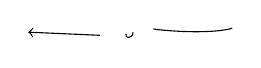
\begin{tikzpicture}[x=1cm,y=1cm]
\draw[<-] (0,.04)--(.91,0);
\draw (1.24,.02) .. controls (1.22,-.045) and (1.33,-.048) .. (1.33,.04);
\draw (1.59,.08) .. controls (1.93,.035) and (2.40,.03) .. (2.59,.09);
\end{tikzpicture}}\endgroup\par}
\end{GelfandAdjacentEvidence}
\begin{GelfandAdjacentEvidence}{GELFAND-P000743}{4}


М. \uwave{Превращение всего этого в числа.}

\SourceFigure{GELFAND-P000743}{parameter-bracket}{%
\par\begingroup\color{black}\GelfandFitDiagram{
\begin{tikzpicture}[x=1cm,y=1cm]
\node[inner sep=4pt] (i) {\(I\subset H\otimes\mathbb C^4\)};
\draw (i.north west)--(i.south west)--(i.south east)--(i.north east);
\end{tikzpicture}}\endgroup\par}
\end{GelfandAdjacentEvidence}
\begin{GelfandAdjacentEvidence}{GELFAND-P000743}{5}

--- параметры многоинстантонного решения

изоморфизм диаграмм приводит к одинаковым решениям.

\SourceFigure{GELFAND-P000743}{diagram-isomorphism}{%
\par\begingroup\color{black}\GelfandFitDiagram{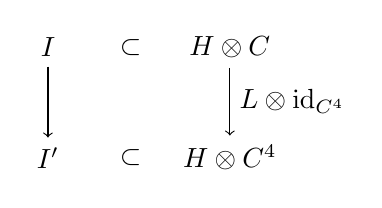
\begin{tikzpicture}[x=1cm,y=1cm]
\node (i) at (0,0) {\(I\)};
\node at (1.05,0) {\(\subset\)};
\node (top) at (2.31,0) {\(H\otimes\mathbb C\)};
\node (j) at (0,-1.40) {\(I'\)};
\node at (1.05,-1.40) {\(\subset\)};
\node (bottom) at (2.31,-1.40) {\(H\otimes\mathbb C^4\)};
\draw[->] (i)--(j);
\draw[->] (top)--node[right]{\(L\otimes\mathrm{id}_{\mathbb C^4}\)}(bottom);
\end{tikzpicture}}\endgroup\par}
\end{GelfandAdjacentEvidence}
\begin{GelfandAdjacentEvidence}{GELFAND-P000743}{6}

\Unclear{GELFAND-P000743}{diagram-upper-space}{Сверху написано \(H\otimes\mathbb C\), снизу \(H\otimes\mathbb C^4\).}
\end{GelfandAdjacentEvidence}
\begin{GelfandAdjacentEvidence}{GELFAND-P000743}{7}


такие изом. диаграмм разрешаются

\(L\) сохр. эрмитову форму.

\uwave{Схема вычисления} \(A_\mu(x)\).

\begin{gather*}
(I\subset H\otimes\mathbb C^4,\quad e_1,\ldots,e_r\ \text{--- базис } I)
\longmapsto 4n\ \text{векторов в }H\\
(e_{ij}),\quad i=1,\ldots,n;\quad j=1,\ldots,4.\\
\dim H=2n+r.
\end{gather*}
\Unclear{GELFAND-P000743}{basis-terminal-index}{Последний индекс в перечне базисных векторов читается предположительно как \(r\).}
\end{GelfandAdjacentEvidence}
\begin{GelfandAdjacentEvidence}{GELFAND-P000743}{8}


Построим по ним матрицу \(\widetilde Q\)

из \((n\times n)\) -блоков размера \(4\times4\)

\((k\ell)\)-й блок на месте \((rs)\) имеем
\[
\underset{\text{числовая матрица}}{Q(e_{kr},e_{\ell s})}
\]
\Unclear{GELFAND-P000743}{form-first-index}{Второй индекс первого аргумента обведён густо. Предположительно \(e_{kr}\).}
\end{GelfandAdjacentEvidence}


Матрица \(\widetilde Q\) задаёт всю ситуацию

\uwave{Предположение}: \(\operatorname{rk}\widetilde Q=2n+r\)
(\(\Leftrightarrow L\) не имеет нетривиальных горизонтальных сечений)
--- опускаем такие вырождения для простоты.


\Needspace{7\baselineskip}
\begin{GelfandAdjacentEvidence}{GELFAND-P000744}{1}
\SourcePage{GELFAND-P000744}{9}

\uwave{Какие \(\widetilde Q\) получаются:}

а) \(\widetilde Q\) эрмитова;

б) \(\operatorname{rk}\widetilde Q=2n+r\);

в) «Условие 0». Это условие на все \(4\times4\) блоки

\SourceFigure{GELFAND-P000744}{block-matrix}{%
\par\begingroup\color{black}\GelfandFitDiagram{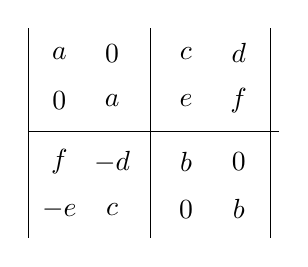
\begin{tikzpicture}[x=.67cm,y=.60cm]
\node at (0,0) {\(a\)}; \node at (1,0) {\(0\)};
\node at (2.4,0) {\(c\)}; \node at (3.4,0) {\(d\)};
\node at (0,-1) {\(0\)}; \node at (1,-1) {\(a\)};
\node at (2.4,-1) {\(e\)}; \node at (3.4,-1) {\(f\)};
\node at (0,-2.3) {\(f\)}; \node at (1,-2.3) {\(-d\)};
\node at (2.4,-2.3) {\(b\)}; \node at (3.4,-2.3) {\(0\)};
\node at (0,-3.3) {\(-e\)}; \node at (1,-3.3) {\(c\)};
\node at (2.4,-3.3) {\(0\)}; \node at (3.4,-3.3) {\(b\)};
\draw (-.59,.53)--(-.59,-3.91);
\draw (1.72,.53)--(1.72,-3.91);
\draw (4.01,.53)--(4.01,-3.91);
\draw (-.59,-1.65)--(4.16,-1.65);
\end{tikzpicture}}\endgroup\par}
\end{GelfandAdjacentEvidence}
\begin{GelfandAdjacentEvidence}{GELFAND-P000744}{2}

на диаг. скалярные;

симметричн. отн. диаг. \Unclear{GELFAND-P000744}{cancelled-word}{Зачёркнутое слово предположительно «блоки». Середина закрыта штрихами.}
\end{GelfandAdjacentEvidence}
\begin{GelfandAdjacentEvidence}{GELFAND-P000744}{3}

связаны как выписано.

\uwave{Условия 1 и 2 опускаются} (они тоже могут быть выписаны).

Дальше используются \(e_{ij}\), но в ур-я они реально не входят.
\[
H\times S^4=L\oplus L^\perp
\]
\(L^\perp\) порождено глобально \(2n\) сечениями расслоения \(M\times S^4\);
\Unclear{GELFAND-P000744}{bundle-letter}{В этой строке читается \(M\times S^4\).}
\end{GelfandAdjacentEvidence}
\begin{GelfandAdjacentEvidence}{GELFAND-P000744}{4}


\begin{align*}
(21)_1\qquad h_{k1}&=(x_2+ix_1)e_{k1}+(x_4-ix_3)e_{k2}+e_{k3}\\
(21)_2\qquad h_{k2}&=-(x_4+ix_3)e_{k1}+(x_2-ix_1)e_{k2}+e_{k4}
\end{align*}

\SourceFigure{GELFAND-P000744}{column-grouping}{%
\par\begingroup\color{black}\GelfandFitDiagram{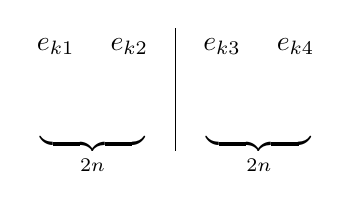
\begin{tikzpicture}[x=.76cm,y=.76cm]
\node at (0,0) {\(e_{k1}\)};
\node at (1.23,0) {\(e_{k2}\)};
\node at (2.78,0) {\(e_{k3}\)};
\node at (4.01,0) {\(e_{k4}\)};
\draw (2,.3)--(2,-1.75);
\node at (.615,-1.8) {\(\underbrace{\hspace{1.33cm}}_{2n}\)};
\node at (3.395,-1.8) {\(\underbrace{\hspace{1.33cm}}_{2n}\)};
\end{tikzpicture}}\endgroup\par}
\end{GelfandAdjacentEvidence}
\begin{GelfandAdjacentEvidence}{GELFAND-P000744}{5}


На бесконечности всё тривиализуется.

«Инстантон живёт недолго и притом в мнимом времени ---\\
--- человекоподобное образование»

Выберем среди \(e_{ij}\) базис \(H\),\qquad \(B\subset(e_{ij})\)

\(\Leftrightarrow\) \((2n+r)\)-диагональный минор в \(\widetilde Q\)

(один такой минор)

По нему разложим систему порождающих сечений \(L\).
\[
(22)\qquad \sum X_b\,Q\bigl(b,\underset{h_{k2}}{h_{k1}}\bigr)=0,\qquad
k=1,\ldots,n,\qquad b\in B.
\]
\Unclear{GELFAND-P000744}{equation22}{\(h_{k2}\) подписано под \(h_{k1}\), ниже скобок.}
\end{GelfandAdjacentEvidence}


это система \(2n\) ур-й для \(2n+r\) неизвестных \(X_b\).

Фунд. система решений \(X^{(i)}\), \(i=1,\ldots,r\).

Ортонормируем её до \([Y^{(i)}]\) и теперь напишем ответ:


\Needspace{7\baselineskip}
\begin{GelfandAdjacentEvidence}{GELFAND-P000745}{1}
\SourcePage{GELFAND-P000745}{unlabelled}

\SourceFigure{GELFAND-P000745}{formula-bracket}{%
\par\begingroup\color{black}\GelfandFitDiagram{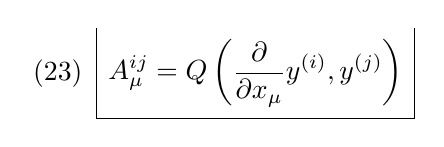
\begin{tikzpicture}
\node[inner sep=4pt] (a) {\(\displaystyle A_\mu^{ij}=Q\left(\frac{\partial}{\partial x_\mu}y^{(i)},y^{(j)}\right)\)};
\node[anchor=east,inner sep=2pt] at ([xshift=-3pt]a.west) {\((23)\)};
\draw (a.north west)--(a.south west)--(a.south east)--(a.north east);
\end{tikzpicture}}\endgroup\par}
\end{GelfandAdjacentEvidence}
\begin{GelfandAdjacentEvidence}{GELFAND-P000745}{2}

\Unclear{GELFAND-P000745}{formula-y-case}{Обе буквы в (23) имеют нижний выносной штрих и читаются как строчные \(y\).}
\end{GelfandAdjacentEvidence}
\begin{GelfandAdjacentEvidence}{GELFAND-P000745}{3}


\(X^{(i)}\) --- рациональные ф-и со значениями в \(H\);

при ортонормировании возникнут корни из рациональных ф-й.

\uwave{Геометрическая теорема}.

Диаграммы \(I\subset H\otimes\mathbb C^4\) с какими-то усл. \ldots

классифицируют расслоения над \(\mathbb{C}P^3\) с условиями.

1) \(H^i(L(-2))=0\) и то же для \(L^*\);
\Unclear{GELFAND-P000745}{cohomology-index}{У верхнего индекса \(i\) видна точка в месте тонкой горизонтальной полосы скана.}
\end{GelfandAdjacentEvidence}


2) \(H^2(L(-1))=0\);

3) \(H^0(L(-1))=0\).


\Needspace{7\baselineskip}
\begin{GelfandAdjacentEvidence}{GELFAND-P000746}{1}
\SourcePage{GELFAND-P000746}{15}

\underline{28/\(\overline{\underline{\mathrm{XI}}}\)-77.}\qquad
\underline{Сем. Гельфанда.}

\fcolorbox{red}{white}{\underline{\underline{Л. Д. Фаддеев.}}}\qquad
\underline{Солитоны как частицы.}

I. \(u(x,t)\) --- поле, \(x\in\mathbb R^d\), \(d=1,2,3\).

\[
\Box=\frac{\partial^2}{\partial t^2}-\frac{\partial^2}{\partial x^2}
\]
\begin{equation*}
\Box u+m^2u+\varepsilon V'(u)=0
\tag{1}
\end{equation*}
\begin{equation*}
\mathcal L=\int\left[\tfrac12\,\partial u\cdot\partial u
-\tfrac12 m^2u^2-\varepsilon V(u)\right]dx
\tag{2}
\end{equation*}
\[
\partial_0u(x,t)\underset{\mathrm{def}}{=}\pi(x,t)
\]
\begin{equation*}
\{u(x,t),\pi(y,t)\}=\delta(x-y)
\tag{3}
\end{equation*}
\begin{equation*}
H=\int\left[\tfrac12\pi^2+\tfrac12(\nabla u)^2
+\tfrac12m^2u^2+\varepsilon V(u)\right]dx
\tag{4}
\end{equation*}

\uwave{Свободное поле}: \(\varepsilon=0\)

В квантовой теории \(u,\pi\) --- операторы.

Преобр. Фурье при \(\varepsilon=0\):
\begin{equation*}
H=\int\sqrt{k^2+m^2}\,a^*(k)a(k)\,dk
\tag{5}
\end{equation*}
\begin{equation*}
\{a^*(k),a(k')\}=i\delta(k-k')
\tag{6}
\end{equation*}

\uwave{Квантование}: пусть \(a,a^*\) --- операторы, оператор
\begin{equation*}
\hat\rho(k)=\hat a^*(k')\hat a(k)
\tag{7}
\end{equation*}
\Unclear{GELFAND-P000746}{eq7-argument}{В первом множителе виден штрих у \(k'\). Во втором множителе у \(k\) штриха нет.}
\end{GelfandAdjacentEvidence}
\begin{GelfandAdjacentEvidence}{GELFAND-P000746}{2}


имеет соб. значения:
\begin{equation*}
\rho'(k)=\sum\left[\delta(k-k_1)+\dots+\delta(k-k_n)\right]
\tag{8}
\end{equation*}
\Unclear{GELFAND-P000746}{eq8-summation}{После знака равенства стоит \(\sum\) без пределов, затем квадратная скобка.}
\end{GelfandAdjacentEvidence}


\uwave{Спектр гамильтониана интерпретируется в терминах частиц}.
\begin{equation*}
E(k_1,\dots,k_n)=\omega(k_1)+\dots+\omega(k_n),\qquad
\omega=\sqrt{k^2+m^2}
\tag{9}
\end{equation*}

(см.: аналогия с осциллятором)


\Needspace{7\baselineskip}
\begin{GelfandAdjacentEvidence}{GELFAND-P000747}{1}
\SourcePage{GELFAND-P000747}{unlabelled}

\uwave{В классич. терминах}: если реш. с конечной энергией ур-я (1) асимптотически приближ. на \(\infty\) к реш. свободного ур-я, то эта картина естественна.
\Unclear{GELFAND-P000747}{top-cancelled-word}{Зачёркнутое слово предположительно «Тогда».}
\end{GelfandAdjacentEvidence}
\begin{GelfandAdjacentEvidence}{GELFAND-P000747}{2}

Тогда \(H(u)=H(u_0)\), т. к. \(H\) --- интеграл.

Солитоны --- контрпример к этой гипотезе.

\uwave{Солитоны}: «всё, что не удовл. условию \(u\to u_0\) при \(|t|\to\infty\)»

«Определение»: \uwave{солитон --- то, что}
\Unclear{GELFAND-P000747}{definition-cancelled-start}{Зачёркнуто, предположительно «не уд».}
\end{GelfandAdjacentEvidence}
\begin{GelfandAdjacentEvidence}{GELFAND-P000747}{3}

\uwave{не расплывается на бесконечности, имея конечную энергию}.

\uwave{Пример}: решение стационарного ур-я.

\(u_s(x)\) --- одно решение \(\Rightarrow\) преобр. Лоренца даёт
\Unclear{GELFAND-P000747}{eq10-deleted-factor}{Перед левой скобкой густо зачёркнута запись. Сверху вписано \(u_s\).}
\end{GelfandAdjacentEvidence}
\begin{GelfandAdjacentEvidence}{GELFAND-P000747}{4}

\begin{equation*}
u_s\left(\frac{x-x_0-vt}{\sqrt{1-v^2}}\right)=u_s(x,t\mid x_0,v)
\tag{10}
\end{equation*}
\Unclear{GELFAND-P000747}{eq10-right-correction}{Возле правого конца дробной черты небольшой зачёркнутый знак. Скобка обведена и продлена вниз.}
\end{GelfandAdjacentEvidence}
\begin{GelfandAdjacentEvidence}{GELFAND-P000747}{5}


уже солитон, завис. от 2-х параметров.

При больших временах: если \(v_1\ne v_2\) то
\begin{equation*}
u(x,t\mid x_{01},v_1)+u(x,t\mid x_{02},v_2)
\tag{11}
\end{equation*}
асимптотически решение.

Тогда асимптотика: при \(|t|\to\infty\)
\begin{equation*}
u\to u_0+\sum u(x,t\mid v_i,x_{0i})
\tag{12}
\end{equation*}
\Unclear{GELFAND-P000747}{eq12-argument-order}{После вертикальной черты написано \(v_i,x_{0i}\).}
\end{GelfandAdjacentEvidence}


(в общем случае --- гипотеза; в моделях --- теорема)

При \(t\to+\infty\) и при \(t\to-\infty\) разные.

Энергия
\begin{equation*}
H(u)=H(u_0)+\sum_{i=1}^{n}H_s(v_i)
\tag{13}
\end{equation*}
По релятив. ф-ле ясно, что
\begin{equation*}
H_s(v)=\frac{M}{\sqrt{1-v^2}}=\sqrt{p^2+M^2}
\qquad\text{(«энергия солитона»)}
\tag{14}
\end{equation*}

\(M\) --- энергия статич. солитона («масса» по определению).

(14) --- определение \(p\).

Получилось 2 части фазового пр-ва. Энергия:
\begin{equation*}
\int\omega(k)\rho(k)\,dk+\sum_i^n\sqrt{p_i^2+M^2}
\tag{15}
\end{equation*}

Солитоны дали вклад ещё в классике. В квантовой механике входит \(\dfrac{M}{\hbar c}\);
солитоны сохраняются при \(\hbar\to+0\).


\Needspace{7\baselineskip}
\begin{GelfandAdjacentEvidence}{GELFAND-P000748}{1}
\SourcePage{GELFAND-P000748}{16}

В квант. механике спектр. будет
\begin{equation*}
\sum_{i=1}^{N}\sqrt{k_i^2+m^2}+\sum_i^n\sqrt{p_i^2+M^2}
\tag{16}
\end{equation*}
Из одного поля 2 сорта частиц (по квазиклассике)

\uwave{Периодич. решение.}
\begin{equation*}
u_p(x,t\mid x_0,\bar v,\beta,\alpha)
\tag{17}
\end{equation*}
\Unclear{GELFAND-P000748}{eq17-beta}{Переписанный знак читается предположительно как \(\beta\).}
\end{GelfandAdjacentEvidence}
\begin{GelfandAdjacentEvidence}{GELFAND-P000748}{2}

\(\beta\) связано с \(T\) (период), \(\alpha\) (нач. фаза) параметры

В этом случае
\begin{equation*}
\sum_{i=1}^{N}\sqrt{k^2+m^2}+\sum_i^n\sqrt{p_i^2+M^2}
+\sum_k^\tau\sqrt{p_k^2+M(\alpha_k)}
\tag{18}
\end{equation*}
\Unclear{GELFAND-P000748}{eq18-first-radicand}{В первом радикале написано \(k^2\), без видимого нижнего индекса.}
\end{GelfandAdjacentEvidence}
\begin{GelfandAdjacentEvidence}{GELFAND-P000748}{3}

\Unclear{GELFAND-P000748}{eq18-upper-index}{Верхний предел последней суммы предположительно \(\tau\). Возможное чтение \(r\).}
\end{GelfandAdjacentEvidence}
\begin{GelfandAdjacentEvidence}{GELFAND-P000748}{4}

\Unclear{GELFAND-P000748}{eq18-last-radicand}{В последнем радикале написано \(M(\alpha_k)\), без видимого показателя \(2\).}
\end{GelfandAdjacentEvidence}
\begin{GelfandAdjacentEvidence}{GELFAND-P000748}{5}


\uwave{Основная модельная задача:}
\begin{equation*}
v(u)=1-\cos u-\frac{u^2}{2}
\tag{19}
\end{equation*}
\Unclear{GELFAND-P000748}{eq19-potential-glyph}{Начальный знак перед \((u)\) передан как \(v\). Возможно \(\upsilon\).}
\end{GelfandAdjacentEvidence}
\begin{GelfandAdjacentEvidence}{GELFAND-P000748}{6}

Ур-е имеет вид:
\begin{equation*}
\Box u+m^2\sin u=0
\tag{20}
\end{equation*}
(ур-е \((\sin\varphi)_2\))

Ещё один параметр: в скобке Пуассона поставим
\begin{equation*}
\{\partial_0u,u\}=\gamma\delta(\ldots)
\tag{21}
\end{equation*}
Тогда оказывается, что
\begin{equation*}
M=\frac{8m}{\gamma}\qquad\text{(«тяжёлая частица»)}
\tag{22}
\end{equation*}
\begin{equation*}
M_2(\alpha)=\frac{16m}{\gamma}\sin\alpha,\qquad 0<\alpha\leq\frac{\pi}{2}.
\tag{23}
\end{equation*}
Этими \Unclear{GELFAND-P000748}{cancelled-word}{Зачёркнутое слово предположительно «двумя».}
\end{GelfandAdjacentEvidence}

решениями всё определяется.

При этом надо брать
\begin{equation*}
\alpha=\frac{\gamma}{16}n,\quad n=1,2,\ldots
\tag{24}
\end{equation*}
(Тахтаджан, \underline{Фаддеев}, \(\approx1974\) г.)

Сейчас должен выйти подробный обзор (по английски).


\Needspace{7\baselineskip}
\begin{GelfandAdjacentEvidence}{GELFAND-P000749}{1}
\SourcePage{GELFAND-P000749}{unlabelled}

\underline{II.} \uwave{Последовательное квантование и \(S\)-матрица}.

Найти настоящие соб. ф-и пока не удалось.
\Unclear{GELFAND-P000749}{eigenfunction-abbreviation}{В первой строке сокращение читается как «соб.».}
\end{GelfandAdjacentEvidence}
\begin{GelfandAdjacentEvidence}{GELFAND-P000749}{2}

 Но \(S\)-матрица вычислена! (обходным путём: континуальный интеграл)

Определения: написать
\begin{equation*}
H=\int\left[\frac{\pi^2}{2}+\frac{(\nabla u)^2}{2}+\frac{m^2}{2}u^2+V(u)\right]
\tag{25}
\end{equation*}
и считаем \(\pi\) и \(u\) операторами с соотношением
\begin{equation*}
[\hat\pi(x),\hat u(y)]=i\delta(x-y)
\tag{26}
\end{equation*}
Противоречия нет, но надо начать с перенормировок.

\uwave{Glimm, Jaffe:}

\uwave{Frohlich}
\Unclear{GELFAND-P000749}{latin-surname}{Средние буквы фамилии не вполне ясны. Предположительное чтение «Frohlich».}
\end{GelfandAdjacentEvidence}
\begin{GelfandAdjacentEvidence}{GELFAND-P000749}{3}

\[
\left[\begin{gathered}
\frac{m^2}{\gamma}(1-\cos\gamma u)\quad\text{при малых }\gamma\quad\text{построили}\\
\text{гамильтониан аккуратно}\quad(\text{при }x\in\mathbb R^1).
\end{gathered}\right.
\]
\Unclear{GELFAND-P000749}{small-coupling}{В знаменателе и перед \(u\) написано \(\gamma\), без видимого показателя \(2\).}
\end{GelfandAdjacentEvidence}
\begin{GelfandAdjacentEvidence}{GELFAND-P000749}{4}


\underline{Лемма 1} (из обычной квант. механики). \uwave{Рассм. ур-е}
\begin{equation*}
i\frac{\partial\Psi}{\partial t}=H\Psi
\tag{27}
\end{equation*}
\begin{equation*}
H=-\frac{\Delta}{2m}+v(x),\quad v\text{ быстро убывает}
\tag{28}
\end{equation*}
\Unclear{GELFAND-P000749}{eq28-potential}{Округлый знак перед \((x)\) и далее передан как \(v\). Возможно \(\upsilon\).}
\end{GelfandAdjacentEvidence}

\uwave{Тогда сущ. предел}
\begin{equation*}
S=\lim_{\substack{t''\to\infty\\t'\to-\infty}}
e^{iH_0t''}e^{-iH(t''-t')}e^{-iH_0t'}
\tag{29}
\end{equation*}
(\(S\)-матрица) \uwave{и} \(S\) --- \uwave{унитарный оператор}.

Лучше считать в импульсном представлении: ядро обозначается \(S(p'',p')\). Достаточно знать ядро опер. эволюции
\(e^{-iH(t''-t')}=K\)
\[
K(x'',t''\mid x',t')
\]
Надо взять
\begin{equation*}
\begin{cases}
x''=\dfrac{p''}{m}t''\\
x'=\dfrac{p'}{m}t'
\end{cases}
\tag{30}
\end{equation*}
(по классическим ф-лам со свободным \(H_0\)). Тогда
\begin{equation*}
S(p'',p')=\lim_{\substack{t''\to+\infty\\t'\to-\infty}}
\frac{K\left(\frac{p''}{m}t'',t''\mid\frac{p'}{m}t',t'\right)}
{K_0\left(\frac{p''}{m}t'',t''\mid0,0\right)
K_0\left(0,0\mid\frac{p'}{m}t',t'\right)}
\tag{31}
\end{equation*}
(аналогична (29))


\Needspace{7\baselineskip}
\begin{GelfandAdjacentEvidence}{GELFAND-P000750}{1}
\SourcePage{GELFAND-P000750}{17}

Правая часть (31) считается континуальным интегралом по траекториям с классическими асимптотиками.

\uwave{Комментарий к} (31): применяем к \(\Psi\), рассматривая волновой пакет
\begin{equation*}
\Psi(x,t)=\left[\frac1{2\pi}\int\Psi(p)e^{ipx}e^{-i\frac{p^2}{2m}t}\,dp\right]
\underset{\substack{\uparrow\\\text{метод стац.}\\\text{фазы}}}{\cong}
\widetilde\Psi\left(\frac{mx}{t}\right)e^{i\frac{x^2}{2mt}}
\tag{32}
\end{equation*}
\Unclear{GELFAND-P000750}{eq32-integrand-psi}{Над знаком \(\Psi\) под интегралом видна короткая отметка. Тильда неясна.}
\end{GelfandAdjacentEvidence}
\begin{GelfandAdjacentEvidence}{GELFAND-P000750}{2}

\Unclear{GELFAND-P000750}{eq32-exponent-overwrite}{Последний знак знаменателя показателя экспоненты густо обведён, предположительно \(t\).}
\end{GelfandAdjacentEvidence}
\begin{GelfandAdjacentEvidence}{GELFAND-P000750}{3}

\[
\Psi(t)=e^{-iH_0t'}\Psi
\]
\Unclear{GELFAND-P000750}{unnumbered-time-argument}{Слева написано \(\Psi(t)\), справа в показателе экспоненты \(t'\).}
\end{GelfandAdjacentEvidence}
\begin{GelfandAdjacentEvidence}{GELFAND-P000750}{4}

Получим
\begin{equation*}
K(.\ .\mid\tfrac{p}{m}t,t)\,\widetilde\Psi(p)\sqrt{\frac mt}\,dp
\tag{33}
\end{equation*}
с множителями (в каждой части переходим в свою систему координат).
\SourceFigure{GELFAND-P000750}{triangle}{%
\par\begingroup\color{black}\GelfandFitDiagram{
\begin{tikzpicture}
\fill (0,0)--(.03,.30)--(.34,.19)--cycle;
\end{tikzpicture}}\endgroup\par}
\end{GelfandAdjacentEvidence}
\begin{GelfandAdjacentEvidence}{GELFAND-P000750}{5}


\underline{Континуальный интеграл.} Сначала для квантовой механики
\begin{equation*}
K(x'',t''\mid x',t')=\frac1N\int
e^{i\int_{t'}^{t''}\left[\frac{m\dot x^2}{2}-v(x)\right]dt}
\prod_{t'\leq t\leq t''}dx(t),
\tag{34}
\end{equation*}
\Unclear{GELFAND-P000750}{eq34-potential}{Начальный знак в \(v(x)\) округлый. Возможно \(\upsilon\).}
\end{GelfandAdjacentEvidence}
\begin{GelfandAdjacentEvidence}{GELFAND-P000750}{6}

по таким траекториям, что
\begin{equation*}
x(t')=x',\quad x(t'')=x''
\tag{35}
\end{equation*}
\(N\) --- нормирующий множитель (зависящий от времени).

Теперь нужно считать, что \(x(t')=\dfrac{pt'}m\), \(x(t'')=\dfrac{pt''}m\).

В теории поля надо написать
\begin{equation*}
K(u''(x),t''\mid u'(x),t')=\frac1N\int
\exp\left\{i\int\mathcal L(x)\,dx\right\}
\prod_{\substack{t'\leq t\leq t''\\-\infty<x<\infty}}
du\,\text{[зачёркнуто]}(x,t)
\tag{36}
\end{equation*}
\Incomplete{GELFAND-P000750}{eq36-cancelled-argument}{После \(du\) зачёркнут фрагмент перед \((x,t)\). Чтение под штрихами не установлено.}
\end{GelfandAdjacentEvidence}
\begin{GelfandAdjacentEvidence}{GELFAND-P000750}{7}

по таким \(u\), что
\begin{equation*}
\begin{cases}
u(x,t'')=u''(x)\\
u(x,t')=u'(x)
\end{cases}
\tag{37}
\end{equation*}
В качестве нач. и конечных конфигураций надо взять суммы по солитонам. Получаются вероятности перехода.

Хорошего квантового варианта обратной задачи пока нет.
\Unclear{GELFAND-P000750}{good-word-crossing}{Тонкий диагональный штрих пересекает конец слова «Хорошего» и уходит вправо вниз.}
\end{GelfandAdjacentEvidence}
\begin{GelfandAdjacentEvidence}{GELFAND-P000750}{8}


Для \(S\)-матрицы sin-Гордона угадана точная формула
(\uwave{Замолодчиков} из ИТЭФ; см. Comm. on Math. Physics)

\Incomplete{GELFAND-P000750}{hypothesis-prefixed-mark}{Перед «Гипотеза» находятся зачёркнутые штрихи с частью прямоугольной рамки. Чтение не установлено.}
\end{GelfandAdjacentEvidence}

Гипотеза: все классич. решаемые задачи решаются и в квантовом варианте


\Needspace{7\baselineskip}
\begin{GelfandAdjacentEvidence}{GELFAND-P000751}{1}
\SourcePage{GELFAND-P000751}{unlabelled}

\begin{equation*}
\langle u''(x)\mid e^{-iH(t''-t')}\mid u'(x)\rangle
\tag{38}
\end{equation*}
--- матр. элемент, задаваемый континуальным интегралом. Теперь надо делить и устремлять \(t\) к \(\pm\infty\).

Поправки к
\Incomplete{GELFAND-P000751}{top-cancel}{Между «к» и «классической» зачёркнут короткий фрагмент. Он не разобран.}
\end{GelfandAdjacentEvidence}
\begin{GelfandAdjacentEvidence}{GELFAND-P000751}{2}

классической массе возникают на уровне одного солитона.

\uwave{Задачи, возникающие при вычислении интеграла.}

Метод стационарной фазы.
\begin{equation*}
u(x,t)=U_{cl}(x,t)+\sqrt h\,\varphi(x,t)+\ldots
\tag{39}
\end{equation*}
\Incomplete{GELFAND-P000751}{cancel-before-operator}{Перед «Возникает оператор» густо зачёркнута фраза. Чтение не установлено.}
\end{GelfandAdjacentEvidence}
\begin{GelfandAdjacentEvidence}{GELFAND-P000751}{3}

Возникает оператор
\begin{equation*}
A\varphi=\Box\varphi+m^2\varphi+V''(u_\varphi)\varphi
\tag{40}
\end{equation*}
\Unclear{GELFAND-P000751}{operator-mass-term}{После \(m^2\) густо обведённые знаки читаются предположительно \(\varphi+\).}
\end{GelfandAdjacentEvidence}
\begin{GelfandAdjacentEvidence}{GELFAND-P000751}{4}

\Unclear{GELFAND-P000751}{operator-u-index}{Нижний знак у \(u\) читается предположительно как \(\varphi\).}
\end{GelfandAdjacentEvidence}
\begin{GelfandAdjacentEvidence}{GELFAND-P000751}{5}

Поправки вычисляются через \(\det A\).

Он выражается через \(S\)-матрицу для вспомогательного линейного уравнения. Дальше петли возникают.
Нужно знать обратный оператор \(R=A^{-1}\) и ядро \underline{\(R(x,y)\)}, а именно
\begin{equation*}
\int R^3(x,x)\,d^2x
\tag{41}
\end{equation*}
\uwave{Надежды}: не исключено, что такие функционалы явно считаются.
\Unclear{GELFAND-P000751}{cancel-quadratures}{Зачёркнуто, предположительно «в квадратурах».}
\end{GelfandAdjacentEvidence}
\begin{GelfandAdjacentEvidence}{GELFAND-P000751}{6}


Пусть \(u_1\) --- односолитонное решение (стационарное),
\begin{equation*}
V''(u_1(x))=q(x).
\tag{42}
\end{equation*}
Вычисление
\begin{equation*}
\det\left(\frac{d^2}{dt^2}-\frac{d^2}{dx^2}+q(x)\right)
\tag{43}
\end{equation*}
сводится к спектр. плотности стац. оператора (переменные разделяются). Получается \(q(x)=\frac1{\operatorname{ch}^2x}\)
и явно находятся все соб. функции (простейший потенциал Баргмана).

\(\det A\) выраж. через соб. ф-ю с нулевым соб. значением.

Поправки к массе
\Incomplete{GELFAND-P000751}{cancel-before-soliton}{Перед «солитона» густо зачёркнуто короткое слово. Чтение не установлено.}
\end{GelfandAdjacentEvidence}
\begin{GelfandAdjacentEvidence}{GELFAND-P000751}{7}

солитона:
\begin{equation*}
M=\frac{8m}{\gamma}-\frac m\pi+O(\gamma)
\tag{44}
\end{equation*}
\underline{Гипотеза}: для sine-Gordon
\begin{equation*}
M=\frac{8m}{\gamma}-\frac m\pi,
\tag{45}
\end{equation*}
т. е. высших поправок нет. (оправд. Замолодчиковым)
\Unclear{GELFAND-P000751}{justified-abbreviation}{Сокращение перед фамилией читается предположительно «оправд.». Первая буква может быть «с».}
\end{GelfandAdjacentEvidence}


При \(\gamma\leq8\pi\) всё хорошо, а дальше солитон исчезает.


\Needspace{7\baselineskip}
\begin{GelfandAdjacentEvidence}{GELFAND-P000752}{1}
\SourcePage{GELFAND-P000752}{18}

\uwave{Формулы \(S\)-матрицы для sin-Гордона.}

Надо Сосчитать укороченное действие для 2-солитонного решения.
\begin{equation*}
S_{sa}(p_1'',p_2'';p_1',p_2')
=\delta(p_1''-p_1')\delta(p_2''-p_2')e^{i\Theta(p_1,p_2)}
\tag{46}
\end{equation*}
\Unclear{GELFAND-P000752}{equation-46-separator}{Разделитель аргументов густо обведён. Предположительно точка с запятой.}
\end{GelfandAdjacentEvidence}
\begin{GelfandAdjacentEvidence}{GELFAND-P000752}{2}

(Есть солитон и антисолитон)

Действие (классическое)
\begin{equation*}
\Theta=\frac8\gamma\int_0^\pi d\alpha
\left[\ln\frac{e^{i(\beta-\alpha)}+1}{e^{i\beta}+e^{-i\alpha}}\right]
\tag{47}
\end{equation*}
[Зачёркнуто: При \(\gamma=\frac{8\pi}{N}\), \(N\) --- целое]
\Incomplete{GELFAND-P000752}{cancel-after-47}{Конец зачёркнутой строки после «целое» не разобран.}
\end{GelfandAdjacentEvidence}
\begin{GelfandAdjacentEvidence}{GELFAND-P000752}{3}

(интеграл не берётся).

Надо взять \(\gamma=\frac{8\pi}{N}\), \(N\) --- целое число
\begin{equation*}
\Theta\longrightarrow\sum\ln(\ldots)
\tag{48}
\end{equation*}
Замолодчиков считал, что это верно для \(\gamma=\frac{8\pi}{N}\) и проинтерполировал.

В результате sin-Гордон оказался похож на квантовомеханич. систему [Зачёркнуто: и] с
\begin{equation*}
H=-\frac{d^2}{dx^2}+\frac{a}{\operatorname{ch}^2\alpha x}
\tag{49}
\end{equation*}
\Unclear{GELFAND-P000752}{potential-numerator}{Числитель предположительно \(a\), возможно \(q\).}
\end{GelfandAdjacentEvidence}
\begin{GelfandAdjacentEvidence}{GELFAND-P000752}{4}

[Зачёркнуто: Соб. значение \(\alpha(\ell+\tfrac12)^2\)]
\Unclear{GELFAND-P000752}{cancel-eigenvalue-formula}{Зачёркнутая формула читается предположительно \(\alpha(\ell+\tfrac12)^2\).}
\end{GelfandAdjacentEvidence}
\begin{GelfandAdjacentEvidence}{GELFAND-P000752}{5}

\Incomplete{GELFAND-P000752}{cancel-eigenvalue-end}{Конец зачёркнутой строки не разобран. Видно предположительно «с пр…».}
\end{GelfandAdjacentEvidence}
\begin{GelfandAdjacentEvidence}{GELFAND-P000752}{6}


\underline{Замечательная дин. система}

связана с полем (киральным)
\begin{equation*}
n(x):R^2\longrightarrow S^n\subset R^{n+1}
\tag{50}
\end{equation*}
\begin{equation*}
\mathcal L=\frac12\int\partial n\cdot\partial n\,dx
\tag{51}
\end{equation*}
нетривиален из-за значений (есть нелинейность).

\(L\)-\(A\) пара написана ([Зачёркнуто: Фоль; надписано: Поль]майер (?); Захаров и Михайлов)
\Unclear{GELFAND-P000752}{name-correction}{Начало фамилии исправлено с предположительного «Фоль» на «Поль».}
\end{GelfandAdjacentEvidence}
\begin{GelfandAdjacentEvidence}{GELFAND-P000752}{7}


[Зачёркнуто: На]
\Incomplete{GELFAND-P000752}{cancel-before-quantization}{Продолжение зачёркнутой фразы перед «Квантование» не разобрано.}
\end{GelfandAdjacentEvidence}

Квантование слабо связано с классикой.

Массивные частицы появляются как солитоны.

По этому поводу будет доклад на сем. им. И. Г. Петровского.


\Needspace{7\baselineskip}
\begin{GelfandAdjacentEvidence}{GELFAND-P000753}{1}
\SourcePage{GELFAND-P000753}{unlabelled}

\underline{13/II-78 г.}\qquad \uwave{Сем. Гельфанда.}

\underline{И. М. Г.} в теории категорий есть 2 перв. понятия:
1) Topos\quad 2) Производная категория.

\SourceFigure{GELFAND-P000753}{speaker-box}{\begingroup\color{black}\GelfandFitDiagram{\begin{tikzpicture}
\node[draw=red,inner sep=3pt,text=black]{\underline{С. Гельфанд}};
\end{tikzpicture}}\endgroup}
\end{GelfandAdjacentEvidence}
\begin{GelfandAdjacentEvidence}{GELFAND-P000753}{2}


\underline{Задача}: описать все алгебраические расслоения над
\Incomplete{GELFAND-P000753}{cancel-before-projective}{Перед обозначением проективного пространства густо зачёркнут короткий знак.}
\end{GelfandAdjacentEvidence}
\begin{GelfandAdjacentEvidence}{GELFAND-P000753}{3}

\(\mathbb P^n\).
(\(n\)-мерное проект. пр-во; например, над \(\mathbb C\)).

\(\Xi\) --- аффинное пр-во.
\[
\xi\sim\alpha\xi,\quad \alpha\in\mathbb C^*,\quad (\xi\ne0);
\qquad \text{Тогда}\ \Xi/{\sim}=\mathbb P^n.
\]
\Unclear{GELFAND-P000753}{scalar-choice}{Множитель и следующий знак читаются предположительно \(\alpha\).}
\end{GelfandAdjacentEvidence}
\begin{GelfandAdjacentEvidence}{GELFAND-P000753}{4}


\(\Lambda\) --- грассманова алгебра от \((n+1)\)-го переменного
(\Incomplete{GELFAND-P000753}{cancel-before-algebra}{В начале скобки густо зачёркнуто сокращение; чтение не установлено.}
\end{GelfandAdjacentEvidence}
\begin{GelfandAdjacentEvidence}{GELFAND-P000753}{5}

алг. над \(\Xi\)).
\[
\Lambda=\{\xi_0,\ldots,\xi_n\mid
\xi_i\xi_j+\xi_j\xi_i=0\}.
\]
\[
\dim\Lambda=2^{n+1}.
\]
Введём на \(\Lambda\) градуировку:
\begin{equation*}
\Lambda=\Lambda_0\oplus\Lambda_{-1}\oplus\cdots\oplus\Lambda_{-(n+1)},
\qquad [\text{Зачёркнуто: }\Lambda_0\text{ --- поле констант}]
\tag{1}
\end{equation*}
где
\[
\Lambda_{-k}\ [\text{Зачёркнуто: }\Lambda_k?]
=\{\xi_{i_1}\cdots\xi_{i_k}\},\qquad
\Lambda_0\text{ --- поле констант}.
\]
\Unclear{GELFAND-P000753}{cancel-grading-symbol}{Перед знаком равенства зачёркнута запись, предположительно \(\Lambda_k\).}
\end{GelfandAdjacentEvidence}
\begin{GelfandAdjacentEvidence}{GELFAND-P000753}{6}


\uwave{Объекты}: градуир. конечномерное представление
\(\Lambda\) или градуир. \(\Lambda\)-модуль:
\begin{equation*}
V=\bigoplus V_j,\qquad \dim V<\infty.
\tag{2}
\end{equation*}
\begin{equation*}
\Lambda_{-k}V_j\subset V_{j-k}.
\tag{3}
\end{equation*}

Пусть \(\xi_0,\ldots,\xi_n\) --- базис в \(\Xi\), \(\xi\in\Xi\).
\begin{equation*}
\xi=c_0\xi_0+\cdots+c_n\xi_n.
\tag{4}
\end{equation*}
\((-k)\) --- по историческим причинам (от статьи Серра).

Тогда \(\xi:V_j\longrightarrow V_{j-1}\).
Отсюда т. к. \(\deg\xi=-1\), то
\SourceFigure{GELFAND-P000753}{complex-diagram}{\begingroup\color{black}\GelfandFitDiagram{\begin{tikzcd}[ampersand replacement=\&,column sep=large]
\cdots\arrow[r]\&V_1\arrow[r,"\xi"]\&V_0\arrow[r,"\xi"]\&
V_{-1}\arrow[r]\&\cdots
\end{tikzcd}}\endgroup}
\end{GelfandAdjacentEvidence}
\begin{GelfandAdjacentEvidence}{GELFAND-P000753}{7}


\(\xi^2=0\ \Rightarrow\) получили комплекс.

Итак, По элементу \(\xi\ne0\) и модулю \(V\) строится комплекс
\begin{equation*}
L_\xi(V)=
\{\cdots\longrightarrow V_1\xrightarrow{\xi}V_0
\xrightarrow{\xi}V_{-1}\longrightarrow\cdots\}.
\tag{5}
\end{equation*}

\uwave{Определение}. \(V\) наз. \dashuline{правильным}, если
\begin{equation*}
\forall\xi\ne0,\qquad H_i(L_\xi(V))=0\quad\text{при }i\ne0.
\tag{6}
\end{equation*}
Здесь:
\begin{equation*}
H_i\ [\text{Зачёркнуто: ?}]\ (L_\xi(V))
=\ker(V_i\longrightarrow V_{i-1})/
\operatorname{Im}(V_{i+1}\longrightarrow V_i)
\tag{7}
\end{equation*}
\Incomplete{GELFAND-P000753}{cancel-homology-symbol}{Между индексом и скобкой в (7) густо зачёркнут знак.}
\end{GelfandAdjacentEvidence}
\begin{GelfandAdjacentEvidence}{GELFAND-P000753}{8}

\Unclear{GELFAND-P000753}{homology-equation-number}{Номер формулы обведён густо; предположительно (7).}
\end{GelfandAdjacentEvidence}
\begin{GelfandAdjacentEvidence}{GELFAND-P000753}{9}


--- [Зачёркнуто: факторпространства?]
\Unclear{GELFAND-P000753}{cancel-homology-word}{Зачёркнутое слово предположительно «факторпространства»; начало закрыто густыми штрихами.}
\end{GelfandAdjacentEvidence}

\uwave{гомологии комплекса}.


\Needspace{7\baselineskip}
\begin{GelfandAdjacentEvidence}{GELFAND-P000754}{1}
\SourcePage{GELFAND-P000754}{43}

В этом случае
\[
\dim H_0^{?}(L_\xi(V))=\mathrm{const}
\]
\Unclear{GELFAND-P000754}{top-homology-mark}{Над \(H_0\) плотный знак, внутренние штрихи которого неразличимы. В наборе отмечен вопросительным знаком.}
\end{GelfandAdjacentEvidence}
\begin{GelfandAdjacentEvidence}{GELFAND-P000754}{2}

(не зависит от \(\xi\))

в силу формулы Эйлера

(лев. часть — эйлерова характеристика \(\xi\)?
\Unclear{GELFAND-P000754}{euler-overwritten-mark}{После «характеристика» переписанный знак, возможно \(\xi\).}
\end{GelfandAdjacentEvidence}
\begin{GelfandAdjacentEvidence}{GELFAND-P000754}{3}

равная \(\sum(-1)^i\dim V_i\).)

Расслоение: \(\xi\longmapsto H_0(L_\xi(V))\).

[Зачёркнуто: Если \(\xi\) и]
\Unclear{GELFAND-P000754}{cancelled-line}{Короткая зачёркнутая строка читается предположительно «Если ξ и».}
\end{GelfandAdjacentEvidence}


Для \(\xi\) и \(\alpha\xi\) одно и то же (есть естеств. изоморфизм).

\uwave{Пример}. \(V=\Lambda\) (регулярное представление).

\(V_j=\Lambda_j\) (градуировка та же, что была).

\uwave{Ответ}:
\(H_i(L_\xi(V))=0,\quad\forall i,\quad\forall\xi\ne0\).

Получаем нулевое расслоение.

Прямые суммы дадут тот же результат.

\(V_j=\Lambda_{j+\ell}\quad(\ell\text{ --- фиксировано})\)

\(\Rightarrow\) снова получаем трив. расслоение.

Отсюда свб. модули приводят к трив. расслоениям.

\uuline{Теорема 1}
\uwave{Любое расслоение получ. такой конструкцией,
причём \(V\) определено однозначно с точностью до добавления свободного модуля.}

(Бернштейн, С. Гельфанд, И. Гельфанд;
независимо близкий рез. Бейлинсон, студ. 3-го курса)

\dashuline{Уточнение конструкции расслоения.}

\(V\) --- произвольный \(\Lambda\)-модуль.

\(O(k)\) --- стандартные расслоения
(их сеч. — однородные рац. ф-и степени \(k\in\mathbb Z\)), одномерные.

Рассмотрим
\begin{equation*}
\mathcal L_j=V_{-j}\otimes O(j).
\tag{8}
\end{equation*}
--- расслоение над \(\mathbb P^n\);
каждый слой умножается на \(V_{-j}\).

\(O(1)\) --- то, у которого есть сечение.

Построим
\begin{equation*}
d:\mathcal L_j\longrightarrow\mathcal L_{j+1}.
\tag{9}
\end{equation*}
\(f(\xi)\) --- сеч. \(\mathcal L_j\) над открытым мн-вом

однор. ф-я степ. \(j\) со знач. в \(V_{-j}\)
\begin{equation*}
d(f(\xi))=\xi(f(\xi)).
\tag{10}
\end{equation*}
(справа действие \(\xi\) на \(V_{-j}\), дающее \(V_{-j-1}\)).


\Needspace{7\baselineskip}
\begin{GelfandAdjacentEvidence}{GELFAND-P000755}{1}
\SourcePage{GELFAND-P000756}{44}

Построим теперь 2 \(\Lambda\)-модули
\begin{equation*}
V=C_N\otimes\Lambda
\tag{18}
\end{equation*}
(на \(C_N\) трив. действие \(\Xi?\);
\Unclear{GELFAND-P000756}{action-overwritten-symbol}{Знак после «действие» густо обведён; чтение \(\Xi\) предположительное.}
\end{GelfandAdjacentEvidence}
\begin{GelfandAdjacentEvidence}{GELFAND-P000756}{2}

на \(\Lambda\) обычное действие)
\begin{equation*}
V'=C_{N+1}\otimes\Lambda.
\tag{\(18'\)}
\end{equation*}
Имеем
\begin{equation*}
\partial:V\longrightarrow V'
\tag{19}
\end{equation*}
\begin{equation*}
\partial(c\otimes\lambda)=\sum_{i=0}^n X_i(c)\otimes\xi_i\lambda
\tag{20}
\end{equation*}
От базиса \(\partial\) не зависит.
Положим \(W=\operatorname{Ker}\partial\).

Это \(\Lambda\)-модуль. Теперь надо сдвинуться обратно \(N\) раз
\[
0\longrightarrow W'\longrightarrow P\longrightarrow W\longrightarrow0
\]
\(W\longmapsto W'\) проделать \(N\) раз
(со сдвигом градуировки).

Это и есть то самое представление (тот самый \(\Lambda\)-модуль)

\underline{И.М.Г.}\quad\uwave{Классиф. расслоений}
--- не совсем прав. задача (не образуют абелеву категорию).
Надо разрешить слоям менять
\Incomplete{GELFAND-P000756}{cancelled-dimension-word}{Между «менять» и «размерность» густо зачёркнуто короткое слово.}
\end{GelfandAdjacentEvidence}
\begin{GelfandAdjacentEvidence}{GELFAND-P000756}{3}

размерность --- ввести пучки.
Излаг. работа — развитие теор. Серра.

\uwave{Теорема Серра}
\[
\{\text{Пучки на }\mathbb CP^n\}\Leftrightarrow
\left\{
\begin{array}{l}
\text{конечно-порожд. }\overset{\text{(градуир.)}}{\text{модули}}\\
\text{над }\mathbb C[x_0,\ldots,x_n]
\end{array}
\Big/
\begin{array}{l}
\text{с точн.}\\
\text{до конечн.}\\
\text{числа однор.}\\
\text{компонент}
\end{array}
\right\}
\]

\(\xi?\)
\Unclear{GELFAND-P000756}{book-left-mark}{Отдельный переписанный знак слева от примечания, возможно \(\xi\); его роль не установлена.}
\end{GelfandAdjacentEvidence}
\begin{GelfandAdjacentEvidence}{GELFAND-P000756}{4}

(статья в сб. “Расслоенные пр-ва”; 1953 года).
\Incomplete{GELFAND-P000756}{book-right-cancellation}{После примечания о сборнике зачёркнут короткий фрагмент.}
\end{GelfandAdjacentEvidence}
\begin{GelfandAdjacentEvidence}{GELFAND-P000756}{5}


Построим пучок по модулю \(M\).

Зададим его сечения над \(E_i=\{x.\ x_i\ne0\}\)

[Зачёркнуто: \(\Gamma(E_i,M)?\)]
\Unclear{GELFAND-P000756}{cancelled-section-formula}{Зачёркнутая формула читается предположительно \(\Gamma(E_i,M)\); диагональные штрихи мешают различить аргументы.}
\end{GelfandAdjacentEvidence}

\[
\Gamma(E_i,\underset{\text{наш пучок}}{L})
=\left\{\frac{m}{x_i^s},\
\begin{array}{l}
\deg m=s\\
m\in M
\end{array}\right\}.
\]

\(O(N)\) возникает из \(M=\mathbb C[x_0,\ldots,x_n]\)
со сдвинутой градуировкой
\[
M_i=\{\mathbb C[x_0,\ldots,x_n]\}_{i+N}.
\]


\Needspace{7\baselineskip}
\begin{GelfandAdjacentEvidence}{GELFAND-P000757}{1}
\SourcePage{GELFAND-P000757}{unlabelled}

\uuline{27/II-78 г.}\qquad \underline{Сем. Гельфанда.}

\SourceFigure{GELFAND-P000757}{speaker-box}{\begingroup\color{black}\GelfandFitDiagram{\begin{tikzpicture}
\node[draw=red,inner sep=3pt,text=black]{\uwave{С. И. Гельфанд}};
\end{tikzpicture}}\endgroup}
\end{GelfandAdjacentEvidence}
\begin{GelfandAdjacentEvidence}{GELFAND-P000757}{2}


\uwave{Задача}: описать алгебраические векторные расслоения над проективным пр-вом.

\(\Xi\) --- \((n+1)\)-мерное пространство (векторное).

\(\mathbb P=\mathbb P(\Xi)\) --- проективное \(n\)-мерное пространство

[Зачёркнуто]
\Incomplete{GELFAND-P000757}{cancelled-word}{Перед «Выберем базис» зачёркнуто короткое слово; цельное чтение не установлено.}
\end{GelfandAdjacentEvidence}

Выберем базис \(\Xi\): \(\xi_0,\ldots,\xi_n\)

и пусть
\[
\Lambda=\Lambda(\Xi)\quad\text{--- внешняя алгебра }\Xi
\]
\[
\Lambda=\bigoplus_{i=-n-1}^{0}\Lambda_i
\]
\(\Lambda\) имеет образующие \(\xi_0,\ldots,\xi_n\) и соотношения
\(\xi_i\xi_j+\xi_j\xi_i=0,\quad\xi_i^2=0;\)
\[
\Lambda_{-k}=\{\xi_{i_1}\ldots\xi_{i_k}\}.
\]


\Needspace{7\baselineskip}
\begin{GelfandAdjacentEvidence}{GELFAND-P000758}{1}
\SourcePage{GELFAND-P000758}{unlabelled}

\[
\dim\Lambda_{-k}=\binom{n+1}{k}
\]
\uwave{Замечание}: пусть \(\xi\in\Lambda_{-1}\).
Тогда \(\xi^2=0\).
(и это эквивалентно всем соотнош.).

\dashuline{Объект}: градуированный конечномерный \(\Lambda\)-модуль
\[
V=\bigoplus_j V_j,\qquad
\lambda\in\Lambda_i,\ v\in V_j\Rightarrow\lambda v\in V_{i+j}
\]
(\(j\) могут быть любые целые).

По каждому \(V\) построим набор векторных расслоений над \(\mathbb P(\Xi)\)
и их отображений (комплекс расслоений).

\(\forall j\) построим расслоения \(O(j)\)

\uwave{3 опред.} \(O(j)\)

1) ф-и перехода \((z_k/z_\ell)^j\);

2) сечения над откр. мн-вом \(=\) однор. рац. ф-и степени \(j\);

3) \(j\)-я тенз. степень антихопфовского расслоения.

Соотв. пучок можно определять так:
\[
\Gamma(O(j),U)=
\{\text{рац. ф-и степени }j\text{ без особ. в }\bar U\}
\]
\(U\subset\mathbb P^n\), \(\bar U\) --- прообраз \(U\) в \(\Xi\)

\uwave{Задача}: почему получается 1-мерное расслоение?

\SourceFigure{GELFAND-P000758}{separator}{\begingroup\color{black}\GelfandFitDiagram{\begin{tikzpicture}
\draw (0,0)--(.62,0);
\fill (.91,0) circle (1pt);
\draw (1.22,0)--(1.96,0);
\end{tikzpicture}}\endgroup}
\end{GelfandAdjacentEvidence}
\begin{GelfandAdjacentEvidence}{GELFAND-P000758}{2}


Положим
\[
\mathcal L^j=V_{-j}\otimes O(j)\qquad\text{--- расслоение.}
\]
\Unclear{GELFAND-P000758}{middle-index-correction}{Нижний индекс у \(\mathcal L\) замазан, сверху написано \(j\). Зачёркнутый нижний индекс предположительно \(j\).}
\end{GelfandAdjacentEvidence}
\begin{GelfandAdjacentEvidence}{GELFAND-P000758}{3}


\(V_{-j}\) означает постоянное расслоение со слоем \(V_{-j}\)
\[
\Gamma(\mathcal L^j,U)=
\left\{\begin{gathered}
\text{рац. ф-и со знач. в }V_{-j},\\
\text{степ. однор. }j,\ \text{неособые в }\bar U
\end{gathered}\right\}.
\]
\Unclear{GELFAND-P000758}{sections-index-correction}{В \(\Gamma(\mathcal L^j,U)\) нижний индекс также замазан, сверху написано \(j\). Зачёркнутый индекс предположительно \(j\).}
\end{GelfandAdjacentEvidence}
\begin{GelfandAdjacentEvidence}{GELFAND-P000758}{4}


Построим отображения:
\[
d:\mathcal L^j\longrightarrow\mathcal L^{j+1}
\]
\dashuline{На сечениях}: пусть
\(f(\xi)\in\Gamma(\mathcal L^j,U)\),
\[
\xi\in\Lambda_{-1}=\Xi
\]
\[
(df)(\xi)=\xi[f(\xi)]
\]
(справа действие \(\xi\) как элемента внешней алгебры на \(V_{-j}\)).

Получается комплекс расслоений:
\[
\mathcal L(V)=\{\mathcal L^j,d\},\qquad d^2=0.
\]

\uwave{Правильный \(\Lambda\)-модуль}:

пусть \(\xi\in\Xi,\quad\xi\ne0\).
[Зачёркнуто: \(\xi'\in\mathbb P\) --- \(\xi'\) соответствующая \(\xi\).]
\Unclear{GELFAND-P000758}{bottom-cancelled-projective-point}{Зачёркнутая запись о проективной точке предположительно читается \(\xi'\in\mathbb P\) — \(\xi'\) соответствующая \(\xi\). Отдельные перечёркнутые знаки не вполне ясны.}
\end{GelfandAdjacentEvidence}


Рассмотрим послед. векторных пр-в (комплекс)
\[
\{\ldots\longrightarrow V_{-j+1}
\xrightarrow{\xi}V_{-j}\xrightarrow{\xi}V_{-j-1}
\longrightarrow\ldots\}=L_\xi.
\]


\Needspace{7\baselineskip}
\begin{GelfandAdjacentEvidence}{GELFAND-P000759}{1}
\SourcePage{GELFAND-P000759}{56}

\underline{Определение}. \(V\) \uwave{правильный}, если
\[
H^i(L_\xi)=0,\quad\forall i\ne0,\quad\forall\xi\ne0.
\]
\(L_\xi\) --- комплекс, полученный из \(\mathcal L(V)\) в точке \(\xi\).

Для правильного \(V\)
\[
\dim H^0(L_\xi)=\mathrm{const}
\]
Пр-ва \(H^0(L_\xi)\) склеиваются в векторное расслоение.
Точное опред. таково: положим
\[
\begin{aligned}
\Phi(V)&=H^0(\mathcal L(V))\\
&=\operatorname{Ker}(d:\mathcal L^0\to\mathcal L^1)
\big/\operatorname{Im}(d:\mathcal L^{-1}\to\mathcal L^0).
\end{aligned}
\]

\underline{Теорема 1}.
1) \uwave{Любое алг. вект. рассл. \(\mathcal E\) имеет вид
\(\Phi(V)\) для нек-рого правильного \(V\).}

2)
\[
\Phi(V)\cong\Phi(V')\Longleftrightarrow
V\oplus P\cong V'\oplus P'
\]
для свободных \(P,P'\).
\Unclear{GELFAND-P000759}{theorem-stable-relation}{Во втором отношении над двумя горизонтальными чертами слабый штрих: предположительно \(\cong\), возможно \(=\).}
\end{GelfandAdjacentEvidence}
\begin{GelfandAdjacentEvidence}{GELFAND-P000759}{2}


\underline{Обратное отображение}.

\uwave{Когерентные пучки модулей на} \(\mathbb P^n\)

(\(=\) фактор-пучки пучков сечений расслоений).

Это удобнее, т.к. можно брать образ, коядро и т.д..

(\(\sim\) присоед. разностей).

\underline{Теорема Серра}:
\[
X=\Xi^*,\qquad S=S(X)\text{ --- алг. многочленов.}
\]
\SourceFigure{GELFAND-P000759}{dual-space-pointer}{\begingroup\color{black}\GelfandFitDiagram{\begin{tikzpicture}
\node[text=black] (dual) at (0,0){\(\Xi^*\)};
\node[text=black] (label) at (1.6,.48){двойств. пр-во};
\draw (dual.north east)--(label.west);
\end{tikzpicture}}\endgroup}
\end{GelfandAdjacentEvidence}
\begin{GelfandAdjacentEvidence}{GELFAND-P000759}{3}


Кат. пучков на \(\mathbb P^n\) (когер.)
[зачёркнуто: по?]
\Unclear{GELFAND-P000759}{serre-cancelled-word}{Зачёркнутое слово перед «эквивал.» предположительно «по», возможно «до».}
\end{GelfandAdjacentEvidence}
\begin{GelfandAdjacentEvidence}{GELFAND-P000759}{4}

\uwave{эквивал.} категории градуированных \(S(X)\)-\uwave{модулей}
с точн. до конечномерных.

\SourceFigure{GELFAND-P000759}{module-insertion}{\begingroup\color{black}\GelfandFitDiagram{\begin{tikzpicture}
\node[text=black] (module) at (0,.65){модулей};
\node[draw,ellipse,text=black,inner sep=3pt] (insert) at (0,0){(с кон. числом образ.)};
\draw (module.south)--(insert.north);
\end{tikzpicture}}\endgroup}
\end{GelfandAdjacentEvidence}
\begin{GelfandAdjacentEvidence}{GELFAND-P000759}{5}


\[
\mathcal E\longmapsto M=\bigoplus M_j,\qquad
M_j=\Gamma(\mathcal E\otimes O(j),\mathbb P^n)
\]
\[
S_k=\Gamma(O(k),\mathbb P^n)
\]
Структура модуля вводится очевидным образом.

\SourceFigure{GELFAND-P000759}{separator}{\begingroup\color{black}\GelfandFitDiagram{\begin{tikzpicture}
\draw (0,0)--(1,0);
\fill (1.34,0) circle (1pt);
\draw (1.64,0)--(2.84,0);
\end{tikzpicture}}\endgroup}
\end{GelfandAdjacentEvidence}
\begin{GelfandAdjacentEvidence}{GELFAND-P000759}{6}


\underline{Доказательство теоремы 1}.

\(1^\circ\).
\uwave{По \(\Lambda\)-модулю \(V\)
строим комплекс \(S\)-модулей}
\(W=(W^k,d)\):
\[
W^k=V_{-k}\otimes_{\mathbb C}S(X)
\]
Пусть \(x_0,\ldots,x_n\) --- базис в \(X\), двойств. к базису в \(\Xi\).
положим
\[
d(v\otimes s)=\sum\xi_i v\otimes x_i s.
\]
\SourceFigure{GELFAND-P000759}{memberships}{\begingroup\color{black}\GelfandFitDiagram{\begin{tikzpicture}
\node[text=black] at (0,.7){\(v\)};
\node[text=black] at (0,.33){\rotatebox{90}{\(\in\)}};
\node[text=black] at (0,0){\(V\)};
\node[text=black] at (1.4,.7){\(s\)};
\node[text=black] at (1.4,.33){\rotatebox{90}{\(\in\)}};
\node[text=black] at (1.4,0){\(S(X)\)};
\end{tikzpicture}}\endgroup}
\end{GelfandAdjacentEvidence}


Легко проверить, что \(d:W^k\to W^{k+1}\) и \(d^2=0\).

В каждом \(W^k\) задаётся градуировка:
\[
(W^k)_j=V_{-k}\otimes S_{j+k}
\]
\(d\) --- морфизм градуир. модулей (он не меняет степени).


\Needspace{7\baselineskip}
\begin{GelfandAdjacentEvidence}{GELFAND-P000760}{1}
\SourcePage{GELFAND-P000760}{unlabelled}

(Это алгебр. вариант данной выше геометрич. конструкции)

\(V\longmapsto\) комплекс расслоений \(\mathcal L(V)\)

\(\overline W\) --- Это алгебр. аналог \(\mathcal L(V)\).
\Unclear{GELFAND-P000760}{w-upper-stroke}{Короткий отдельный штрих над левой частью \(W\) передан как надчёркивание.}
\end{GelfandAdjacentEvidence}
\begin{GelfandAdjacentEvidence}{GELFAND-P000760}{2}


\uwave{Обобщение}: рассмотрим комплекс \(\Lambda\)-модулей
\[
\ldots\xrightarrow{\partial}V^i\xrightarrow{\partial}V^{i+1}
\xrightarrow{\partial}V^{i+2}\xrightarrow{\partial}\ldots
\]
\uwave{Неточно}: построим \(W^{i,k}\) (бикомплекс) и сумма по диагоналям

(комплекс по бикомплексу)
\[
V^i=\bigoplus(V^i)_j;\qquad
W^k_j=\bigoplus_{\ell} V^{\ell+k}_{j-\ell}\otimes S_\ell
\]
\[
d(v\otimes s)=\partial v\otimes s+\sum\xi_i v\otimes x_i s
\]
\Unclear{GELFAND-P000760}{total-differential-sign}{Между слагаемыми стоит плюс. Перед суммой дополнительного знакового множителя не видно.}
\end{GelfandAdjacentEvidence}
\begin{GelfandAdjacentEvidence}{GELFAND-P000760}{3}


Он не меняет [зачёркнуто: его?]
\Unclear{GELFAND-P000760}{cancelled-before-lower-index}{Короткая зачёркнутая запись может читаться «его» или \(j\).}
\end{GelfandAdjacentEvidence}
\begin{GelfandAdjacentEvidence}{GELFAND-P000760}{4}

нижн. индекс, а верхний — на 1 увелич..

\SourceFigure{GELFAND-P000760}{separator}{\begingroup\color{black}\GelfandFitDiagram{\begin{tikzpicture}
\draw (0,0)--(.8,0);
\fill (1.14,0) circle (1pt);
\draw (1.45,0)--(2.55,0);
\end{tikzpicture}}\endgroup}
\end{GelfandAdjacentEvidence}
\begin{GelfandAdjacentEvidence}{GELFAND-P000760}{5}


\(2^\circ\).
\uwave{Комплекс градуир. \(S\)-модулей}
\(\longmapsto\)
\uwave{компл. градуир. \(\Lambda\)-модулей}
\[
\ldots\longrightarrow W^k\xrightarrow{d}W^{k+1}\xrightarrow{d}\ldots
\]

Положим \(\underline{\overline W}=\bigoplus W^k\)
\Unclear{GELFAND-P000760}{total-w-stroke}{На этот раз \(W\) подчёркнуто, и над его левой частью есть ещё короткий штрих.}
\end{GelfandAdjacentEvidence}
\begin{GelfandAdjacentEvidence}{GELFAND-P000760}{6}

и \(\underline V=\operatorname{Hom}_{\mathbb C}(\Lambda,W)\)

Введём градуировку в \(\underline V\):
\[
v\in V^i_j\Longleftrightarrow v(\Lambda_k)\subset W_{j+k}^{i-j-k}
\quad\text{для всех }k.
\]

Положим:
\[
\partial:V^i\longrightarrow V^{i+1}
\]
\[
\partial(v)(\lambda)=d(v(\lambda))+\sum x_i v(\xi_i\lambda)
\]
\uwave{Это отобр. в нек-ром смысле обратно предыдущему.}

\SourceFigure{GELFAND-P000760}{comparison}{\begingroup\color{black}\GelfandFitDiagram{\begin{tikzpicture}
\node[text=black] at (0,0) {\(\begin{array}{ccc}
\text{“}S\text{-модули”}&\longleftrightarrow&\text{“}\Lambda\text{-модули”}\\
\text{(комплексы)}&&\text{(комплексы)}\\
\text{симм.}&\longleftrightarrow&\text{кососимм.}\\
\text{бозе}&\longleftrightarrow&\text{ферми}\\
\text{беск.-мерн.}&\longleftrightarrow&\text{конечномерн.}
\end{array}\)};
\end{tikzpicture}}\endgroup}
\end{GelfandAdjacentEvidence}
\begin{GelfandAdjacentEvidence}{GELFAND-P000760}{7}


\(2^\circ\). \(C^b(\Lambda)\) --- категория компл. конечной длины из \(\Lambda\)-модулей.
\SourceFigure{GELFAND-P000760}{graded-insertion}{\begingroup\color{black}\GelfandFitDiagram{\begin{tikzpicture}
\node[text=black] (grade) at (0,.65){градуир.};
\node[text=black] at (.5,0){из \(\Lambda\)-модулей};
\draw (-.58,.54) to[out=-82,in=157] (-.05,.31) to[out=-27,in=93] (.06,.17);
\draw (.57,.54) to[out=-98,in=25] (.17,.31) to[out=-154,in=84] (.06,.17);
\end{tikzpicture}}\endgroup}
\end{GelfandAdjacentEvidence}


\(C^b(S)\) --- \rule{1em}{.35pt} “ \rule{1.5em}{.35pt}
из конечно-порожд. градуир. \(S\)-модулей

(дифф. сохр. градуировку)


\Needspace{7\baselineskip}
\begin{GelfandAdjacentEvidence}{GELFAND-P000761}{1}
\SourcePage{GELFAND-P000761}{57}

\(C(\Lambda)\) --- категория беск. комплексов град. \(\Lambda\)-модулей
(но бесконечномерных)

Построены функторы:
\begin{align*}
F:\ C^b(\Lambda)&\longrightarrow C^b(S)\\
V&\longmapsto W\qquad(\text{см. п. }1^\circ).
\end{align*}
\Unclear{GELFAND-P000761}{functor-w-stroke}{Левый верхний штрих касается \(W\), поэтому он передан как часть буквы.}
\end{GelfandAdjacentEvidence}
\begin{GelfandAdjacentEvidence}{GELFAND-P000761}{2}

\[
G:\ C^b(S)\longrightarrow C(\Lambda)\qquad(\text{см. п. }2^\circ).
\]

\underline{Основная}\quad\underline{технич.}\quad\underline{теорема}.

\uwave{Рассмотрим естеств. вложение}
\(i:C^b(\Lambda)\longrightarrow C(\Lambda)\).
\uwave{Существует морфизм функторов}
\(i\longrightarrow G\circ F\),
\uwave{индуцирующий изоморфизм когомологий}.

Это значит, что имеется естеств. отображение
\begin{gather*}
\varphi: V\rightsquigarrow\operatorname{Hom}(\Lambda,S\otimes V)\\
\varphi(v):\quad 1\rightsquigarrow\sum x_i\otimes\xi_i v.
\end{gather*}
\Unclear{GELFAND-P000761}{natural-map-source-convention}{В рукописи значение при \(1\) записано как \(\sum x_i\otimes\xi_i v\).}
\end{GelfandAdjacentEvidence}
\begin{GelfandAdjacentEvidence}{GELFAND-P000761}{3}


(\(\forall V\) надо постр. гомом.
\Incomplete{GELFAND-P000761}{map-cancelled-symbol}{После «гомом.» густо зачёркнут знак.}
\end{GelfandAdjacentEvidence}
\begin{GelfandAdjacentEvidence}{GELFAND-P000761}{4}

\(V\longrightarrow G\circ F(V)\))

\(V\) --- 1-мерн. трив. модуль \(\Rightarrow\) справа комплекс Кошуля.

\SourceFigure{GELFAND-P000761}{separator}{\begingroup\color{black}\GelfandFitDiagram{\begin{tikzpicture}
\draw (0,0)--(.9,0);
\fill (1.11,0) circle (1pt);
\draw (1.32,0)--(2.61,0);
\end{tikzpicture}}\endgroup}
\end{GelfandAdjacentEvidence}
\begin{GelfandAdjacentEvidence}{GELFAND-P000761}{5}


\(A\) --- категория (абелева),
\(C(A)\) --- категория комплексов над \(A\) (бесконечных)

\SourceFigure{GELFAND-P000761}{chain-map}{\begingroup\color{black}\GelfandFitDiagram{\begin{tikzcd}[ampersand replacement=\&,column sep=small,row sep=small]
X^\bullet=\{\ldots\arrow[r,"d"] \& X^i\arrow[r,"d"]\arrow[d,"f^i"] \&
X^{i+1}\arrow[r,"d"]\arrow[d,"f^{i+1}"] \& \ldots\}\\
Y^\bullet=\{\ldots\arrow[r] \& Y^i\arrow[r,"d"] \& Y^{i+1}\arrow[r] \& \ldots\}
\end{tikzcd}}\endgroup}
\end{GelfandAdjacentEvidence}
\begin{GelfandAdjacentEvidence}{GELFAND-P000761}{6}

морфизм \(\{f^i\}\) --- диагр. \uwave{коммутативна}.

Когомологии:
\[
H^i(X^\bullet)=\ker d/\operatorname{Im}d
\]

отобр.
\[
X^\bullet\xrightarrow{f}Y^\bullet
\rightsquigarrow f_i^*:H^i(X^\bullet)\longrightarrow H^i(Y^\bullet)
\]
\(f\) наз. \uwave{квазиизоморфизмом}, если оно индуц. изом. всех когомологий.

\underline{Грубо}: производная кат. получ. обращением квазиизоморфизмов.

\uwave{Точное определение}.

\(S\) --- множество квазиизоморфизмов.\qquad (“ensemble” у Вердье)
\[
\operatorname{Ob}(D(A))=\operatorname{Ob}(C(A))
\]
\(\operatorname{Hom}_{D(A)}(X,Y)\) ---
[зачёркнуто: тройки?]
\Unclear{GELFAND-P000761}{roof-cancelled-word}{Зачёркнутое слово предположительно «тройки». Выше в обводке «из троек:».}
\end{GelfandAdjacentEvidence}
\begin{GelfandAdjacentEvidence}{GELFAND-P000761}{7}

[надписано в обводке: из троек:]
\SourceFigure{GELFAND-P000761}{roof-diagram}{\begingroup\color{black}\GelfandFitDiagram{\begin{tikzcd}[ampersand replacement=\&,column sep=small,row sep=small]
Z\arrow[d,"S\ni s"']\arrow[dr,"f"] \& {}\\
X \& Y
\end{tikzcd}}\endgroup}
\end{GelfandAdjacentEvidence}



\Needspace{7\baselineskip}
\begin{GelfandAdjacentEvidence}{GELFAND-P000762}{1}
\SourcePage{GELFAND-P000762}{unlabelled}

[Зачёркнуто: 2 тройки наз. эквив., если]

Отобр. троек: коммут. диаграмма.
\SourceFigure{GELFAND-P000762}{roof-comparison}{\begingroup\color{black}\GelfandFitDiagram{\begin{tikzcd}[ampersand replacement=\&,row sep=large,column sep=large]
Z\arrow[d,"s"']\arrow[dr,"f",near end] \&
Z'\arrow[l,"S\ni s_1"']\arrow[dl,"s'"',near start]\arrow[d,"f'"]\\
X \& Y
\end{tikzcd}}\endgroup}
\end{GelfandAdjacentEvidence}
\begin{GelfandAdjacentEvidence}{GELFAND-P000762}{2}


\(\operatorname{Hom}_{D(A)}(X,Y)\) --- инд. предел по таким тройкам.

Элемент:
\[
Z\longleftarrow Z'\longleftarrow Z''\longleftarrow\cdots
\]
отождествл., если с нек-рого места совпадают

\underline{2 места, где изл.}:

1) \underline{Hartshorne}\qquad\underline{20}\quad\underline{вып.}\quad\underline{L.N.}

\uwave{Residues and duality}

2) \underline{Verdier}\quad автореф дисс. (1963), перепеч.?
\Unclear{GELFAND-P000762}{verdier-reprint-abbreviation}{Сокращение между датой и «в 569 вып.» предположительно «перепеч.».}
\end{GelfandAdjacentEvidence}
\begin{GelfandAdjacentEvidence}{GELFAND-P000762}{3}

в 569 вып. \uuline{Lect.Notes}

(здесь нет док-в)

\underline{Более общая констр} (аксиом.)
\SourceFigure{GELFAND-P000762}{upper-divider}{\begingroup\color{black}\GelfandFitDiagram{\begin{tikzpicture}
\draw (0,0)--(.8,0);
\fill (1.03,0) circle (1pt);
\draw (1.28,0)--(2.15,0);
\end{tikzpicture}}\endgroup}
\end{GelfandAdjacentEvidence}
\begin{GelfandAdjacentEvidence}{GELFAND-P000762}{4}


[Зачёркнуто: А…]
\Incomplete{GELFAND-P000762}{axioms-cancelled-heading}{В зачёркнутом заголовке различима начальная «А». Остаток закрыт густыми штрихами.}
\end{GelfandAdjacentEvidence}
\begin{GelfandAdjacentEvidence}{GELFAND-P000762}{5}


[На левом поле: (для квазиизм. выполнимы)]
\Unclear{GELFAND-P000762}{axioms-margin-abbreviation}{Конец полевого сокращения «квазиизм.» читается предположительно.}
\end{GelfandAdjacentEvidence}
\begin{GelfandAdjacentEvidence}{GELFAND-P000762}{6}


1)
\[
\left.
\begin{gathered}
s_1\in S,\quad s_2\in S\\
s_1s_2\text{ --- сущ}
\end{gathered}
\right\}\Rightarrow s_1s_2\in S.
\]

2)
\SourceFigure{GELFAND-P000762}{ore-square}{\begingroup\color{black}\GelfandFitDiagram{\begin{tikzcd}[ampersand replacement=\&,column sep=small,row sep=small]
P\arrow[r,"g"]\arrow[d,"s'"] \& Y\arrow[d,"s"]\\
Z\arrow[r,"f"] \& X
\end{tikzcd}}\endgroup}
\end{GelfandAdjacentEvidence}
\begin{GelfandAdjacentEvidence}{GELFAND-P000762}{7}

\[
\begin{gathered}
\forall\ Z,X,Y,\ f,s\\
\exists\ P,g,s'
\end{gathered}
\]

3) Пусть \(f:X\longrightarrow Y\). Тогда эквив. св-ва
\begin{align*}
\text{(i)}\qquad&\exists\ s\in S:\ sf=0\\
\text{(ii)}\qquad&\exists\ s'\in S:\ fs'=0
\end{align*}

\SourceFigure{GELFAND-P000762}{lower-divider}{\begingroup\color{black}\GelfandFitDiagram{\begin{tikzpicture}
\draw (0,0)--(.9,0);
\fill (1.18,0) circle (1pt);
\draw (1.43,0)--(2.37,0);
\end{tikzpicture}}\endgroup}
\end{GelfandAdjacentEvidence}


\uwave{Что надо для постр. морфизма функторов?}

(нужного нам).

1) Строится.

2) Надо пров., что для 1-мерного \(V\) всё в порядке
(простые вычисл. с комплексом Кошуля)

3) Ввести фильтрации, факторы стандартны.

Произв. категория: редукция к факторам.


\Needspace{7\baselineskip}
\begin{GelfandAdjacentEvidence}{GELFAND-P000763}{1}
\SourcePage{GELFAND-P000763}{62}

6/III--78 г.\quad\underline{Сем. Гельфанда.}

[\uuline{И. М. Г.}] Пучок \(C^\infty\)-ф-й \uwave{на} \((-1,1)\),
обр. в \(0\) в точке \(0\) --- пучок сеч. вект. расслоения?

\SourceFigure{GELFAND-P000763}{multiplication-diagram}{%
\par\begingroup\color{black}\GelfandFitDiagram{\begin{tikzpicture}[every node/.style={font=\scriptsize},x=1cm,y=1cm]
\node (label) at (0,0) {$Mx:$};
\node (domain) at (1.35,0) {$C^\infty(a,b)$};
\node (range) at (3.55,0) {$C^\infty_{(0)}(a,b)$};
\draw[->] (domain.east)--(range.west);
\node[anchor=west] at (-.25,-.64) {\uwave{умн. на} \(x\)};
\foreach \x in {.80,3.00} {
  \draw (\x,-.25)--++(1.1,0) (\x,-.42)--++(1.1,0);
  \draw (\x,-.42) --++(.14,.17) --++(.14,-.17)
   --++(.14,.17) --++(.14,-.17) --++(.14,.17)
   --++(.14,-.17) --++(.14,.17);
}
\end{tikzpicture}}\endgroup\par
изом. \(\underline{\underline{C^\infty(a,b)}}\)-модулей.}
\end{GelfandAdjacentEvidence}
\begin{GelfandAdjacentEvidence}{GELFAND-P000763}{2}


\SourceFigure{GELFAND-P000763}{speaker-box}{%
\tikz[baseline=(speaker.base)]{\node[draw=red,text=black,inner sep=2pt] (speaker) {\uuline{Аомото}};}}
\end{GelfandAdjacentEvidence}
\begin{GelfandAdjacentEvidence}{GELFAND-P000763}{3}


\underline{Точно решаемые модели в нейтральных массивных теориях поля}. (на \(\mathbb R^2\))
\Unclear{GELFAND-P000763}{title-ending}{Конечная «х» в «нейтральных» наведена повторно.}
\end{GelfandAdjacentEvidence}
\begin{GelfandAdjacentEvidence}{GELFAND-P000763}{4}


\uwave{3 типа полей}.

\(1^\circ\). \uwave{Вспомогат. фермионы} (на \(\mathbb R\))

\uwave{на} \(\mathbb R\); \(u\in\mathbb R\); поля ковар. по отн. к действию \(\mathbb R^+\) на \(\mathbb R\);

\(\psi(u)^+\) и \(\psi(u)\) --- опер. рожд. и уничтожения;
\begin{equation*}
\tag{1}
\psi(-u)=\psi^+(u);
\end{equation*}
\begin{equation*}
\tag{2}
[\psi(u),\psi(u')]_+=2\pi|u|\delta(u+u');
\end{equation*}
\Unclear{GELFAND-P000763}{eq2-u-marks}{Над \(u\) в модуле видны короткие раздельные штрихи. Отдельный знак не установлен.}
\end{GelfandAdjacentEvidence}
\begin{GelfandAdjacentEvidence}{GELFAND-P000763}{5}


лев. ч. \(\underset{\mathrm{def}}{=}\psi(u)\psi(u')+\psi(u')\psi(u),\)

\(2^\circ\). \uwave{\(\varphi_F(x),\ \varphi^F(x)\)}. (\uwave{на} \(\mathbb R^2\))

Рассмотрим пару функций:
\[
w(x)=(w_+(x),w_-(x))
\]
\begin{equation*}
\tag{3}
\frac{\partial w_\pm}{\partial x^\pm}\mp m w_\mp(x)=0,
\end{equation*}
(ур-е Дирака)\qquad (2 ур-я), \(m\) --- число.

где
\[
x^\pm=\frac{x^0\pm x^1}{2},\qquad p^\pm=p^0\pm p^1.
\]
\begin{equation*}
\tag{4}
\langle w,w'\rangle=\int_{-\infty}^{\infty}dx^1
\bigl(w_+(x)w'_+(x)+w_-(x)w'_-(x)\bigr)
\end{equation*}
\begin{equation*}
\tag{5}
\psi_\pm(x)=\int_{-\infty}^{\infty}\underline{du}\,
\sqrt{0+iu}^{\,\pm}\psi(u)
\exp\!\left(-im\left(x^-u+\frac{x^+}{u}\right)\right),
\end{equation*}
\Unclear{GELFAND-P000763}{eq5-small-oval}{Над правой скобкой виден небольшой овал. Его значение не установлено.}
\end{GelfandAdjacentEvidence}
\begin{GelfandAdjacentEvidence}{GELFAND-P000763}{6}


\SourceFigure{GELFAND-P000763}{pairing-margin}{%
\par(ф-я от \(x^0\) --- времени)\par
\(\Vert\) \(\langle w,w'\rangle\) не зависит от \(x^0\) в силу ур-й.}
\end{GelfandAdjacentEvidence}


Здесь
\[
\underline{du}=\frac{du}{2\pi|u|}
\]


\Needspace{7\baselineskip}
\begin{GelfandAdjacentEvidence}{GELFAND-P000764}{1}
\SourcePage{GELFAND-P000764}{unlabelled}

\(\pm\) над корнем --- выбор ветви \(+0\) или \(-0\)
\begin{equation*}
\tag{6}
w(x)\longleftrightarrow\int_{-\infty}^{\infty}dx^1
(w_+\psi_++w_-\psi_-)=\psi(x^0,w)
\end{equation*}
\Unclear{GELFAND-P000764}{eq6-corrected-argument}{В первом аргументе после \(x\) видна плотная правка, над которой различим \(0\). Чтение \(x^0\) предположительно.}
\end{GelfandAdjacentEvidence}
\begin{GelfandAdjacentEvidence}{GELFAND-P000764}{2}


Это уже оператор

Имеет место ортог. разложение пр-ва решений:
\begin{equation*}
\tag{7}
W=\left\{w\ \middle|\ \frac{\partial w_\pm}{\partial x^\pm}\mp m w_\mp=0\right\}
=W_x^+\oplus W_x^-,
\end{equation*}
где
\begin{equation*}
\tag*{\((8)_1\)}
W_x^+=\{w\in W\mid w=0\text{ в области заштрих.}\}
\end{equation*}
\SourceFigure{GELFAND-P000764}{cone-left}{%
\par\begingroup\color{black}\GelfandFitDiagram{\begin{tikzpicture}[scale=1.0]
\begin{scope}
\clip (-.9,.9)--(0,0)--(-.9,-.75)--cycle;
\foreach \k in {-1.8,-1.6,...,.4} {\draw[thin] (\k,-1.1)--++(1.7,2.2);}
\foreach \k in {-.85,-.65,...,-.05} {\draw[thin] (\k,-.75)--++(0,1.65);}
\end{scope}
\draw[->] (-.88,-.76)--(.97,.92) node[above right] {$x^+$};
\draw[->] (.55,-.7)--(-.9,.9) node[above] {$x^-$};
\node at (0,-.50) {$x$};
\end{tikzpicture}}\endgroup}
\end{GelfandAdjacentEvidence}
\begin{GelfandAdjacentEvidence}{GELFAND-P000764}{3}


\begin{equation*}
\tag*{\((8)_2\)}
W_x^-=\{\ldots\mid w=0\text{ в заштр. обл.}\}.
\end{equation*}
\SourceFigure{GELFAND-P000764}{cone-right}{%
\par\begingroup\color{black}\GelfandFitDiagram{\begin{tikzpicture}[scale=1.0]
\begin{scope}
\clip (0,0)--(.96,.78)--(1.19,-.18)--(.66,-.86)--cycle;
\foreach \k in {-1.0,-.8,...,1.2} {\draw[thin] (\k,-1.1)--++(1.45,2.2);}
\foreach \k in {-.2,.03,...,1.65} {\draw[thin] (\k,-1.1)--++(-.50,2.2);}
\end{scope}
\draw (-.9,-.70)--(.96,.78);
\draw (-.56,.63)--(.66,-.86);
\node at (.01,.32) {$x$};
\end{tikzpicture}}\endgroup}
\end{GelfandAdjacentEvidence}
\begin{GelfandAdjacentEvidence}{GELFAND-P000764}{4}


Если бы не ферми, а бозе, то ф-и --- аналог лагранжева разложения на \(p\) и \(q\) (на 2 лагр. плоскости).

\(A(W)\) --- [Зачёркнуто: …] Клиффордова алгебра над \(W\)
\Incomplete{GELFAND-P000764}{clifford-cancelled-word}{Короткая зачёркнутая запись перед «Клиффордова» закрыта наклонными штрихами.}
\end{GelfandAdjacentEvidence}
\begin{GelfandAdjacentEvidence}{GELFAND-P000764}{5}

\[
\{\psi_\mu^\pm\}\quad\text{--- базисы в }W_x^\pm
\]
Клифф. алг. порожд. ими с соотн.
\begin{equation*}
\tag*{\((9)_1\)}
\psi_\mu^+\psi_\nu^-+\psi_\nu^-\psi_\mu^+
\underset{\mathrm{def}}{=}[\psi_\mu^+,\psi_\nu^-]=\delta_{\mu\nu}
\end{equation*}
\begin{equation*}
\tag*{\((9)_2\)}
[\psi_\mu^+,\psi_\nu^+]=[\psi_\mu^-,\psi_\nu^-]=0
\end{equation*}
\Unclear{GELFAND-P000764}{eq9-last-superscript}{Верхний знак у последней \(\psi_\nu\) густо зачёркнут. Минус передан предположительно.}
\end{GelfandAdjacentEvidence}
\begin{GelfandAdjacentEvidence}{GELFAND-P000764}{6}


\uwave{Обозначение}:
\[
\underline{\underline{\psi_\mu^-=\psi_\mu}}
\]

\uwave{Соотношение}:
\begin{equation*}
\tag{10}
A(W)=\Lambda(W_x^+)\cdot\Lambda(W_x)
\end{equation*}
\Unclear{GELFAND-P000764}{eq10-second-factor}{Во втором множителе \(\Lambda(W_x)\) виден нижний индекс \(x\), без верхнего знака.}
\end{GelfandAdjacentEvidence}


Базисы ортогональные отн. скал. произведения (4).

Есть отображение:
\[
\begin{aligned}
A(W)&\longrightarrow\Lambda W_x^+\wedge\Lambda W_x^-\qquad\text{изоморфизм}\\
\lambda\cdot\mu&\overset{N}{\longrightarrow}\lambda\wedge\mu
\end{aligned}
\]
обратное отображение:
\[
{:}\varphi{:}\ \longleftarrow\ \varphi
\]
(произведение Вика)

В бозе-случае это „символ оператора“.


\Needspace{7\baselineskip}
\begin{GelfandAdjacentEvidence}{GELFAND-P000765}{1}
\SourcePage{GELFAND-P000765}{63}

\underline{Определение.}
\[
\varphi_F(x)\in A(W)
\]
\[
\operatorname{Spin}(W_x)=\{g\in A(W_x)\mid gW_xg^{-1}\subset W_x\}
\]
На самом деле
\[
\varphi_F(x)\in\operatorname{Spin}(W)
\]
Есть отображение:
\begin{equation*}
\tag{11}
\operatorname{Spin}(W)\overset{T}{\longrightarrow}O(W);
\qquad\text{а именно:}\quad T_gw=gwg^{-1};
\end{equation*}
[Зачёркнуто: а …]
\Incomplete{GELFAND-P000765}{eq11-cancelled}{Между \(O(W)\) и \(T_gw\) различимы «а» и знак, возможно \(T(g)\). Остаток записи густо зачёркнут. «а именно:» вписано сверху.}
\end{GelfandAdjacentEvidence}
\begin{GelfandAdjacentEvidence}{GELFAND-P000765}{2}


\(W\) имеет скал. произв. и, след., определено \(O(W)\).
\begin{equation*}
\tag{12}
T_{\varphi_F(x)}(w^++w^-)\underset{\mathrm{def}}{=}w^+-w^-
\end{equation*}
(это определение \(\varphi_F(x)\)).

\(T\) не мономорфно; поэтому пока некорр. опред. Точнее,
\begin{equation*}
\tag{13}
\varphi_F(x)={:}\exp L_F(x){:}
\end{equation*}
где
\begin{equation*}
\tag{14}
\begin{aligned}
\Lambda W\ni L_F(x)={}&
\frac12\int_{-\infty}^{\infty}\int_{-\infty}^{\infty}
\underline{du}\,\underline{du'}\,\frac{-i(u-u')}{u+u'-i0}\cdot
\Psi(u)\Psi(u')\\
&{}\qquad\exp\biggl(-im\biggl(x^-(u+u')+{}\\
&\hphantom{{}\qquad\exp\biggl(-im\biggl(}{}+
x^+\biggl(\frac1u+\frac1{u'}\biggr)\biggr)\biggr).
\end{aligned}
\end{equation*}
[Зачёркнуто: Можно говорить?]
\Unclear{GELFAND-P000765}{eq14-cancelled-words}{Под (14) два густо зачёркнутых слова. Чтение «Можно говорить» предположительно.}
\end{GelfandAdjacentEvidence}
\begin{GelfandAdjacentEvidence}{GELFAND-P000765}{3}


Далее,

[Зачёркнуто: …]
\Incomplete{GELFAND-P000765}{eq15-cancelled-symbol}{Слева над (15) знак закрыт густыми наклонными штрихами.}
\end{GelfandAdjacentEvidence}
\begin{GelfandAdjacentEvidence}{GELFAND-P000765}{4}

\begin{equation*}
\tag{15}
\varphi^F(x)=\Psi_0(x)\exp L_F(x),
\end{equation*}
где
\begin{equation*}
\tag{16}
W\ni\Psi_0(x)=\int_{-\infty}^{\infty}\underline{du}\,\Psi(u)
\exp\biggl(-im\biggl(x^-u+\frac{x^+}{u}\biggr)\biggr)
\end{equation*}

Есть [Зачёркнуто: векторы?] 2 объекта:
\Unclear{GELFAND-P000765}{vacuum-cancelled-word}{Зачёркнутое слово перед «2 объекта» предположительно читается «векторы».}
\end{GelfandAdjacentEvidence}

\[
\langle \mathrm{vac}|,\qquad |\mathrm{vac}\rangle
\]
\begin{equation*}
\tag*{\((17)_1\)}
A(W)/A(W)W_x^-=|\mathrm{vac}\rangle
\end{equation*}
\begin{equation*}
\tag*{\((17)_2\)}
W_x^+A(W)\backslash A(W)=\langle\mathrm{vac}|
\end{equation*}
Свойства:
\begin{equation*}
\tag{18}
W_x^-|\mathrm{vac}\rangle=0,\qquad\langle\mathrm{vac}|W_x^+=0
\end{equation*}
(естественные для вакуума).

Рассмотрим функцию
\begin{equation*}
\tag{19}
\langle\mathrm{vac}|\Psi(x_1)\ldots
\Psi(x_k)\varphi_F(a_1)\ldots\varphi_F(a_m)|\mathrm{vac}\rangle;
\end{equation*}
(\(\Psi(x)\) из формулы (6)).

определённую на \((\mathbb R^2)^k\)

Все \(a_\nu\) фиксированы.

(2-мерн. модель Изинга ?)


\Needspace{7\baselineskip}
\begin{GelfandAdjacentEvidence}{GELFAND-P000766}{1}
\SourcePage{GELFAND-P000766}{unlabelled}

\(\underline{\underline{k=1}}\quad\Rightarrow\)
\begin{equation*}
\tag{20}
\langle\mathrm{vac}|\Psi(x)\varphi_F(a_1)\cdot\varphi^F(a_i)
\ldots\varphi_F(a_n)|\mathrm{vac}\rangle
\underset{\mathrm{def}}{=}W^i_{F,n}(x)
\end{equation*}
\uwave{Получается система ур-й}; положим
\begin{equation*}
\tag{21}
M_F=z\partial_z-\bar z\partial_{\bar z}+\frac12
\begin{pmatrix}1&0\\0&-1\end{pmatrix}
\end{equation*}
1-е ур-е имеет вид:
\begin{equation*}
\tag{22}
M_Fw=(Bm^{-1}\partial_z-\bar Bm^{-1}\partial_{\bar z}+E)w
\end{equation*}
\[
z=(x^0+x^1),\qquad\bar z=(x^0-x^1)
\]
\(B,E\) --- пост. матрицы

2-е ур-е
\begin{equation*}
\tag{23}
(m-\Gamma)w=0,\qquad\Gamma=\begin{pmatrix}0&1\\1&0\end{pmatrix}
\end{equation*}
\Unclear{GELFAND-P000766}{eq23-scalar-m}{В (23) перед \(\Gamma\) написано \(m-\).}
\end{GelfandAdjacentEvidence}
\begin{GelfandAdjacentEvidence}{GELFAND-P000766}{2}

\[
w_i=\begin{pmatrix}w_{i+}\\w_{i-}\end{pmatrix},\qquad
\begin{pmatrix}w_1\\w_n\end{pmatrix}
\]
\Unclear{GELFAND-P000766}{eq23-column-end}{В нижнем элементе правого столбца индекс читается как \(n\).}
\end{GelfandAdjacentEvidence}
\begin{GelfandAdjacentEvidence}{GELFAND-P000766}{3}


(22)--(23) --- система максимально переопред.

(на самом деле это связность Гаусса--Манина).

Рассмотрим ещё
\begin{equation*}
\tag{24}
\langle\mathrm{vac}|\varphi_F(a_1)\ldots\varphi_F(a_n)|\mathrm{vac}\rangle=\tau
\end{equation*}
как функцию от \(a\). (\(\tau\)-ф-я)

При \(n=2\) это ф-я Пенлеве 3-го рода.

[Под «Пенлеве» вписано: \underline{(Painleve)}]

\uwave{Wu, Mc Coy, Tracy}, Phys. Rev. B 13 (1976)

[Под фамилиями] что-то о ф-ях Пенлеве.

\uuline{И. М. Г.}

\uwave{Garnier} --- мемуар о ф-ях Пенлеве.

6 типов ур-й; 2-й пор.; особые точки неподвижны; самое общее
\begin{equation*}
\tag{\text{А}}
\begin{aligned}
\frac1y y''={}&\frac a{x^2}+\frac b{(x-1)^2}+\frac c{(x-t)^2}
+\frac d{x(x-1)}+\frac3{4(x-\lambda)^2}\\
&{}+\frac\alpha{x(x-1)(x-t)}+\frac\beta{x(x-1)(x-\lambda)}
\end{aligned}
\end{equation*}
Периоды (монодр.) не зависят от параметров \(\Leftrightarrow\)
\begin{equation*}
\tag{\text{Б}}
\begin{aligned}
\Leftrightarrow\quad\lambda''={}&\frac12
\biggl(\frac1\lambda+\frac1{\lambda-1}+\frac1{\lambda-t}\biggr)(\lambda')^2\\
&{}-\biggl(\frac1t+\frac1{t-1}\mathbin{[?]}
\frac1{t-\lambda}\biggr)\lambda'+{}\\
&{}+2\frac{\lambda(\lambda-1)(\lambda-t)}{t^2(t-1)^2}
\biggl[a+b+c+d+1-\biggl(a+\frac14\biggr)\frac{1}{\lambda^2}\\
&\qquad{}+\biggl(b+\frac14\biggr)\frac{t-1}{(\lambda-1)^2}
-\frac{ct(t-1)}{(\lambda-t)^2}\biggr]
\end{aligned}
\end{equation*}
\Unclear{GELFAND-P000766}{eqb-overwritten-sign}{Между \(1/(t-1)\) и \(1/(t-\lambda)\) знак закрыт густой правкой.}
\end{GelfandAdjacentEvidence}
\begin{GelfandAdjacentEvidence}{GELFAND-P000766}{4}

\Unclear{GELFAND-P000766}{eqb-first-numerator}{В числителе первого члена с \(\lambda^2\) написано \(1\).}
\end{GelfandAdjacentEvidence}


У них одних --- неподв. особые точки.

Постоянство матр. монодромии (А) \(\Leftrightarrow\) неподв. особых точек (Б)

\(t\), \(\lambda\) меняются соглас. с (Б)


\Needspace{7\baselineskip}
\begin{GelfandAdjacentEvidence}{GELFAND-P000767}{1}
\SourcePage{GELFAND-P000767}{unlabelled}

\SourceFigure{GELFAND-P000767}{date-notation}{%
\(\underline{13/\overline{\underline{\mathrm{III}}}-78}\)
\quad\underline{Сем. Гельфанда}}
\end{GelfandAdjacentEvidence}
\begin{GelfandAdjacentEvidence}{GELFAND-P000767}{2}


\SourceFigure{GELFAND-P000767}{aomoto-box}{%
\tikz[baseline=(speaker.base)]{\node[draw=red,text=black,inner sep=2pt] (speaker) {\uuline{Аомото}};}.}
\end{GelfandAdjacentEvidence}
\begin{GelfandAdjacentEvidence}{GELFAND-P000767}{3}


\underline{Об обобщ. классич. гипергеом. ф-и с пом. интегралов}

\underline{типа}\quad\underline{Бернштейна} (И.)
\Unclear{GELFAND-P000767}{bernstein-initial}{После «Бернштейна» в скобках стоит «И.». Сокращение оставлено без раскрытия.}
\end{GelfandAdjacentEvidence}


\par\noindent
\begin{tabular}{@{}p{.27\linewidth}||p{.64\linewidth}@{}}
\uwave{Ф-я Аппеля}.\par Случай 2-х перем.. &
И. М. Г.\par \uwave{Классич. гипергеом. ф-я}:
{\small
\[
\sum_{n=0}^{\infty}x^n
\frac{\alpha(\alpha+1)\ldots(\alpha+n-1)\,\beta(\beta+1)\ldots(\beta+n-1)}
{\gamma(\gamma+1)\ldots(\gamma+n-1)\,n!}
\]
}
\end{tabular}


\Needspace{7\baselineskip}
\begin{GelfandAdjacentEvidence}{GELFAND-P000768}{1}
\SourcePage{GELFAND-P000768}{unlabelled}

\begin{equation*}
\tag{1}
F_1=\sum_{m,n\geq 0}
\frac{(\alpha,m+n)(\beta,m)(\beta',n)}
{(\gamma,m+n)(1,m)(1,n)}x^m y^n
\end{equation*}

\begin{center}---\quad\(\cdot\)\quad---\end{center}

\underline{И. М. Г.}\quad\underline{Од.? опр. гипергеом. ф-и:}
\Unclear{GELFAND-P000768}{upper-heading}{Первое сокращение перед «опр.» читается предположительно как «Од.».}
\end{GelfandAdjacentEvidence}
\begin{GelfandAdjacentEvidence}{GELFAND-P000768}{2}

\[
\begin{gathered}
\bigl((x^2-1)^n\bigr)^{(n)}\qquad\text{(полин. Лежандра)}\\
\Vert\\
\bigl[((x-1)(x+1))^n\bigr]^{(n)}
\end{gathered}
\]

\uwave{Обобщение}:
\[
\bigl[(x-1)^{\alpha-1}(x+1)^{\beta-1}\bigr]^{(\gamma)}
\]

Интегралы порядка \(\alpha\).
\[
I_\alpha f=\int_0^x\frac{(x-t)^{\alpha-1}}{\underbrace{(\alpha-1)!}_{\Gamma(\alpha)}}f(t)\,dt,
\qquad D^\alpha=I_{-\alpha}\quad\text{(аналитич. прод.)}
\]
\[
\bigl[x^{\alpha-1}(1-x)^{\beta-1}\bigr]^{(\gamma)}
\]

Гипергеом. ф-я: 1) хор. разл. в ряды\quad
2) хорошее дифф. ур-е\quad
3) хороший интеграл.
\[
\int_0^x t^{\alpha-1}(1-t)^{\beta-1}(x-t)^{\gamma-1}\,dt
\]

\(B\)-ф-и проще.

\begin{center}---\quad\(\cdot\)\quad---\end{center}

\[
(\alpha,n)=\alpha(\alpha+1)\ldots(\alpha+n-1)
\]
\begin{equation*}
\tag{2}
F_4=\sum_{m,n\geq 0}
\frac{(\alpha,m+n)(\beta,m+n)}
{(\gamma,m)(\gamma',n)(1,m)(1,n)}
\end{equation*}
\Unclear{GELFAND-P000768}{series-f4}{В (2) после дроби множитель \(x^m y^n\) не написан.}
\end{GelfandAdjacentEvidence}
\begin{GelfandAdjacentEvidence}{GELFAND-P000768}{3}


Имеется интегральное представление [Зачёркнуто: …] для \(F_1\)
\Incomplete{GELFAND-P000768}{lower-heading-cancellation}{Короткий знак перед «для \(F_1\)» закрыт наклонными штрихами.}
\end{GelfandAdjacentEvidence}
\begin{GelfandAdjacentEvidence}{GELFAND-P000768}{4}


(3)
\SourceFigure{GELFAND-P000768}{diagram-01}{%
\par\begingroup\color{black}\GelfandFitDiagram{\begin{tikzpicture}[x=1cm,y=1cm]
\draw (.64,.20)--(.96,2.88);
\draw (.58,2.75)--(1.69,.30);
\draw (.04,2.34)--(3.18,.86);
\draw (.13,1.10)--(3.62,1.38)--(3.52,1.45);
\node at (.36,.48) {$1$};
\node at (1.94,.24) {$2$};
\node at (3.01,.46) {$3$};
\node at (3.98,1.13) {$4$};
\end{tikzpicture}}\endgroup\par
У правого конца прямой 4 виден короткий отгиб. Его назначение неясно.}
\end{GelfandAdjacentEvidence}
\begin{GelfandAdjacentEvidence}{GELFAND-P000768}{5}


\[
\int f_1^{\lambda_1}f_2^{\lambda_2}f_3^{\lambda_3}f_4^{\lambda_4}\,da\,db
\]
\Unclear{GELFAND-P000768}{integral-differential}{В \(db\) видны наложенные петли. Чтение \(b\) предположительно.}
\end{GelfandAdjacentEvidence}
\begin{GelfandAdjacentEvidence}{GELFAND-P000768}{6}


\(f_j\) --- лин. формы; \(x,y\) сод. среди коэффициентов.

3 прямые прив. к прост. виду (афф. преобр.) и фиксируются

4-я зад. параметрами \(a,b\).

\(F_2,F_3\) получ. аналогично, но с другим [Зачёркнуто: расп.?] расп. прямых, (не общего полож.):
\Unclear{GELFAND-P000768}{lower-cancelled-word}{Зачёркнутое слово предположительно начинается с «расп».}
\end{GelfandAdjacentEvidence}
\begin{GelfandAdjacentEvidence}{GELFAND-P000768}{7}

[Зачёркнуто: \(F_1\)?]
\Unclear{GELFAND-P000768}{bottom-cancellation}{Внизу слева зачёркнута буква, похожая на \(F\), с коротким штрихом справа внизу. \(F_1\) --- предположительное чтение.}
\end{GelfandAdjacentEvidence}
\begin{GelfandAdjacentEvidence}{GELFAND-P000768}{8}

\SourceFigure{GELFAND-P000768}{diagram-02}{%
\par\begingroup\color{black}\GelfandFitDiagram{\begin{tikzpicture}[x=1cm,y=1cm]
\draw (.55,.07)--(.70,1.60)--(.87,2.65);
\draw (1.49,.07)--(1.67,1.62);
\draw (.04,.35)--(2.88,.57);
\draw (.16,.94)--(2.61,1.11);
\draw (.53,2.46)--(.67,2.34);
\draw (.88,2.16)--(1.67,1.62)--(3.11,.07);
\end{tikzpicture}}\endgroup}
\end{GelfandAdjacentEvidence}



\Needspace{7\baselineskip}
\begin{GelfandAdjacentEvidence}{GELFAND-P000769}{1}
\SourcePage{GELFAND-P000769}{68}

\(F_4:\)
\SourceFigure{GELFAND-P000769}{F4-conic}{%
\par\begingroup\color{black}\GelfandFitDiagram{\begin{tikzpicture}[x=1cm,y=1cm]
\draw (0,0) ellipse (.62 and .46);
\draw (-.73,-.59)--(.73,.64);
\draw (-.70,.59)--(.70,-.54);
\end{tikzpicture}}\endgroup}
\end{GelfandAdjacentEvidence}
\begin{GelfandAdjacentEvidence}{GELFAND-P000769}{2}

вместо 2-х прямых берётся квадр. форма.

\uwave{Число лин. независ. реш. соотв. дифф. ур-й = числу огранич. связных компонент соотв. картины.}

\uwave{Общее замеч. о коэфф.}: отношение соседних = рац. ф-я от \(m,n\).

[Зачёркнуто: …]
\Incomplete{GELFAND-P000769}{cancelled-opening}{Начальные слова перед «Аналогичную задачу» закрыты густыми горизонтальными и косыми штрихами.}
\end{GelfandAdjacentEvidence}
\begin{GelfandAdjacentEvidence}{GELFAND-P000769}{3}

Аналогичную задачу можно делать с любым числом гиперплоскостей
\begin{equation*}
\tag{4}
f_i=\sum_{\nu=1}^{n}a_{i\nu}x_\nu+a_{i0}
\end{equation*}
\[
1\le i\le m
\]
\[
f_{m+1}=1\qquad\text{Обычно }m\ge n.
\]
Рассмотрим матрицу из набора коэффициентов форм
\begin{equation*}
\tag{5}
A=\begin{pmatrix}
a_{10}&\ldots&&a_{1n}\\
\vdots&&&\\
a_{m0}&\ldots&&a_{mn}\\
1&\ldots&0&0
\end{pmatrix}
\in\mathbb C^{m(n+1)}
\end{equation*}
Там действует афф. группа от \(n\) переменных

(на \(x\) она действует)

--- Замена переменного по \(x\)

Пусть
\[
\mathcal M\subset\mathbb C^{m(n+1)}\times\mathbb C^n
\]
состоит из пар
\[
\{(A,x):f_j(x)\ne0\}\qquad\text{(не удовл. ни одно ур-е)}
\]
(дополн. ко всем гиперплоскостям)

\SourceFigure{GELFAND-P000769}{projection-space}{%
\par\begingroup\color{black}\GelfandFitDiagram{\begin{tikzcd}[ampersand replacement=\&]
\mathbb C^{m(n+1)}\times\mathbb C^n\arrow[d,"\pi"]\\
\mathbb C^{m(n+1)}
\end{tikzcd}}\endgroup}
\end{GelfandAdjacentEvidence}
\begin{GelfandAdjacentEvidence}{GELFAND-P000769}{4}


\[
\gamma\subset\mathcal M
\]
м-во таких ур-й, что гиперпл. не в общем положении

\(\underline{\text{ранг}\le n}\)
\Unclear{GELFAND-P000769}{rank-correction}{Неравенство после «ранг» переписано густыми штрихами. Чтение \(\le n\) предположительно.}
\end{GelfandAdjacentEvidence}
\begin{GelfandAdjacentEvidence}{GELFAND-P000769}{5}


\[
[i_1\ldots i_{n+1}]=
\begin{vmatrix}
a_{i_1 0}&\ldots&a_{i_1 n}\\
\vdots&&\\
a_{i_n 0}&&i_n n
\end{vmatrix}
\qquad\text{(минор, получ. из строк }i_1,\ldots,i_n\text{)}
\]
\Unclear{GELFAND-P000769}{minor-indices}{В скобке слева \(i_{n+1}\), в последней строке и пояснении \(i_n\). Нижний правый элемент написан \(i_n n\).}
\end{GelfandAdjacentEvidence}
\begin{GelfandAdjacentEvidence}{GELFAND-P000769}{6}


Проекция [Зачёркнуто: \(\gamma\)?] \(\gamma\) зад. усл. на миноры:
\Unclear{GELFAND-P000769}{projection-cancelled-symbol}{После «Проекция» перед чистой \(\gamma\) зачёркнут знак с петлёй, возможно \(\gamma\).}
\end{GelfandAdjacentEvidence}
\begin{GelfandAdjacentEvidence}{GELFAND-P000769}{7}

\begin{equation*}
\tag{6}
Y=\{A\mid[i_1,\ldots,i_{n+1}]=0\}
\end{equation*}
\SourceFigure{GELFAND-P000769}{projection-gamma}{%
\par\begingroup\color{black}\GelfandFitDiagram{\begin{tikzcd}[ampersand replacement=\&]
\gamma\arrow[d,"\pi"]\\
Y
\end{tikzcd}}\endgroup}
\end{GelfandAdjacentEvidence}
\begin{GelfandAdjacentEvidence}{GELFAND-P000769}{8}

\Unclear{GELFAND-P000769}{bottom-cancelled-symbol}{Под (6) слева отдельно стоит густо обведённый знак, предположительно \(\gamma\).}
\end{GelfandAdjacentEvidence}



\Needspace{7\baselineskip}
\begin{GelfandAdjacentEvidence}{GELFAND-P000770}{1}
\SourcePage{GELFAND-P000770}{unlabelled}

\SourceFigure{GELFAND-P000770}{fibre-leader}{%
\par\begingroup\color{black}\GelfandFitDiagram{\begin{tikzpicture}[every node/.style={font=\scriptsize}]
\node at (-1.0,0) {\(\pi^{-1}(A)\cong\mathbb C^n\setminus\)};
\node (set) at (1.15,0) {\(S_A\)};
\node at (3.0,0) {\(,\quad A\in X\setminus Y\)};
\node[text width=5cm,align=center] (explanation) at (1.15,-1.0) {объед. \(m\) гиперпл. общего положения};
\draw (set.south)--(explanation.north);
\end{tikzpicture}}\endgroup}
\end{GelfandAdjacentEvidence}
\begin{GelfandAdjacentEvidence}{GELFAND-P000770}{2}


\(\Omega_A^\bullet\) --- комплекс рац. форм в \(\mathbb C^n\) с полюсами на \(S_A\)

(внешнее диффер.)

\(\forall\varphi\in\Omega_A\) есть ф-ла
\[
U=f_1^{\lambda_1}\ldots f_m^{\lambda_m},
\]
\SourceFigure{GELFAND-P000770}{connection-brace}{%
{\scriptsize
\[
d_x(U\varphi)=U\underbrace{(\omega\wedge\varphi+d_x\varphi)}_{=\nabla_\omega\varphi},
\]
}
}
\end{GelfandAdjacentEvidence}
\begin{GelfandAdjacentEvidence}{GELFAND-P000770}{3}


Здесь
\[
\omega=\sum_{1}^{m}\lambda_j\frac{df_j}{f_j}
\qquad(\nabla_\omega\text{ --- связность}).
\]
\(\omega\) --- форма связности
\[
\nabla_\omega:\Omega_A^p\longrightarrow\Omega_A^{p+1}
\]
\[
\nabla_\omega\varphi=\omega\wedge\varphi+d_x\varphi
\]
(связность в тривиальном расслоении)

Имеем:
\[
d\omega+\omega\wedge\omega=0
\]
(усл. интегрируемости)

Отсюда вытекает, что \(\nabla_\omega^2=0\) и мы получаем комплекс.

\uwave{Делинь, Гротендик}: возник. теория рац. гиперкогомологий де Рама.

\underline{Предположение.}
\[
\lambda_{m+1}=-\lambda_1-\ldots-\lambda_m
\]
\(\forall\) наб.
\[
1\le i_1<\ldots<i_\nu\le m+1,\qquad1\le\nu\le n.
\]
\uwave{Условие}:
\[
\lambda_{i_1}+\ldots+\lambda_{i_\nu}\notin\mathbb Z^+
\qquad
\mathbb Z^+=\{n\in\mathbb Z,\ n>0\}
\]

\underline{Предл..}
\[
H^p(\Omega_A,\nabla_\omega)=0,\quad p\ne n
\]
\[
\begin{aligned}
H^n(\Omega_A,\nabla_\omega)
&=\chi(\mathbb C^n\setminus S_A)\\
&\cong\frac{
\underset{\substack{=\ \mathrm{def}\\\Omega^n(\log\langle S\rangle)}}{
\left\{\dfrac{df_{i_1}}{f_{i_1}}\wedge\ldots\wedge\dfrac{df_{i_n}}{f_{i_n}}\right\}}
}{\omega\wedge\Omega^{n-1}(\log\langle S\rangle)}
\end{aligned}
\]
\Unclear{GELFAND-P000770}{cohomology-euler}{В рукописи \(H^n(\Omega_A,\nabla_\omega)=\chi(\mathbb C^n\setminus S_A)\). Перед \(H^n\) знак \(\dim\) не написан.}
\end{GelfandAdjacentEvidence}



\Needspace{7\baselineskip}
\begin{GelfandAdjacentEvidence}{GELFAND-P000771}{1}
\SourcePage{GELFAND-P000771}{69}

\underline{Пояснение:}
\[
\Omega^1(\log\langle S\rangle)=\left\{\frac{df_i}{f_i}\right\}_{i\le m}
\]
\[
\bigwedge\Omega^1(\log\langle S\rangle)/\sim\ =\Omega^\bullet(\log\langle S\rangle)
\]
\SourceFigure{GELFAND-P000771}{logarithmic-complex}{%
\par\begingroup\color{black}\GelfandFitDiagram{\begin{tikzcd}[ampersand replacement=\&,column sep=small]
0\arrow[r]\&\mathbb C\arrow[r,"\omega\wedge"]\&\Lambda^1\arrow[r,"\omega\wedge"]\&
\cdots\arrow[r,"\omega\wedge"]\&\Lambda^n\arrow[r]\&0
\end{tikzcd}}\endgroup}
\end{GelfandAdjacentEvidence}
\begin{GelfandAdjacentEvidence}{GELFAND-P000771}{2}


(Они замкнуты: \(\nabla_\omega=\omega\wedge\) для таких форм)
\[
\begin{aligned}
\chi(\mathbb C^n\setminus S_A)&=\binom{m-1}{n}\\
&=\text{число (относит.) компактных связных}
\end{aligned}
\]
компонент \(\mathbb R^n\setminus S_A\)
\Unclear{GELFAND-P000771}{euler-count}{Перед \(\binom{m-1}{n}\) в рукописи нет дополнительного знакового множителя.}
\end{GelfandAdjacentEvidence}
\begin{GelfandAdjacentEvidence}{GELFAND-P000771}{3}

\Unclear{GELFAND-P000771}{compact-insertion}{«(относит.)» вставлено над строкой перед «компактных».}
\end{GelfandAdjacentEvidence}
\begin{GelfandAdjacentEvidence}{GELFAND-P000771}{4}


\begin{center}--- , ---\end{center}

\(\displaystyle\int U\varphi\)\qquad [Зачёркнуто: …]\quad Двойственность

\(\varphi\in\Omega_A\)
\Incomplete{GELFAND-P000771}{cancelled-duality}{Короткая запись между интегралом и «Двойственность» густо зачёркнута.}
\end{GelfandAdjacentEvidence}
\begin{GelfandAdjacentEvidence}{GELFAND-P000771}{5}


\(U\) многозначна \(\Rightarrow\) при обходе получаем предс. фунд. группы:
\[
\ell_U:\pi_1(\mathbb C^n-S_A)\longrightarrow\mathbb C^*
\]
(при обходе умн. на ненулевое компл. число)

Пусть взята соотв. лок. система
\[
\zeta_\ell\text{ --- лок. система},\qquad
\zeta_\ell^*\text{ --- дуальная}.
\]
\Unclear{GELFAND-P000771}{local-system-symbol}{Петлеобразное обозначение локальной системы с индексом \(\ell\) передано предположительно как \(\zeta_\ell\).}
\end{GelfandAdjacentEvidence}
\begin{GelfandAdjacentEvidence}{GELFAND-P000771}{6}


Есть двойств.
\[
H^n(\mathbb C^n\setminus S_A,\zeta_\ell)\times
H_n(\mathbb C^n-S_A,\zeta_\ell^*)\longrightarrow\mathbb C
\]

\(\forall\) комп. связной компоненте \(\longrightarrow\) эл \(\in\)
\[
H_n(\mathbb C^n-S_A,\zeta_\ell)
\]
\Unclear{GELFAND-P000771}{component-coefficient}{Последний знак локальной системы сильно обведён. Отдельная звёздочка, в отличие от предыдущего спаривания, неразличима.}
\end{GelfandAdjacentEvidence}



\Needspace{7\baselineskip}
\begin{GelfandAdjacentEvidence}{GELFAND-P000772}{1}
\SourcePage{GELFAND-P000772}{unlabelled}

\uuline{20/III--78 г.}\qquad\underline{Сем. Гельфанда}

\SourceFigure{GELFAND-P000772}{speaker-box}{%
\par\begingroup\color{black}\GelfandFitDiagram{\begin{tikzpicture}[baseline=(speaker.base)]
\node[draw=red,rectangle,inner sep=4pt] (speaker) {В. М. Бухштабер.};
\draw ([yshift=-2pt]speaker.south west)--([yshift=-2pt]speaker.south east);
\end{tikzpicture}}\endgroup}
\end{GelfandAdjacentEvidence}
\begin{GelfandAdjacentEvidence}{GELFAND-P000772}{2}


(+ А. В. Шокуров)
\Unclear{GELFAND-P000772}{co-speaker}{Начертание фамилии после «А. В.» предположительно читается «Шокуров».}
\end{GelfandAdjacentEvidence}
\begin{GelfandAdjacentEvidence}{GELFAND-P000772}{3}


\underline{Алгебры Ландвебера--Новикова и форм. вект. полей на прямой.}
[Зачёркнуто: …]
\Incomplete{GELFAND-P000772}{title-cancellation}{Небольшая запись под заглавием закрыта густыми штрихами.}
\end{GelfandAdjacentEvidence}
\begin{GelfandAdjacentEvidence}{GELFAND-P000772}{4}


\(\mathbb R^1\), \(\operatorname{Diff}_1\) --- форм. диффеом. прямой с доп. условием: \(\varphi'(0)=1\)
\[
\varphi(0)=0,\qquad\varphi'(0)=1
\]

Группа \(=\underset{\longleftarrow}{\lim}\) конечномерных групп

(в струях пор. \(n\))

Алг. Ли --- алг. Ли форм. вект. полей на \(\mathbb R^1\) --- это \(L_1\).
\[
t+a_1t^2+\ldots+a_nt^{n+1}+\ldots
\]
\(a_j\) --- координаты.

Кольцо функций: \(\underline P\) (полиномы от всех \(a_j\)).
\Unclear{GELFAND-P000772}{function-ring}{Название кольца записано как \(P\) с нижним штрихом.}
\end{GelfandAdjacentEvidence}
\begin{GelfandAdjacentEvidence}{GELFAND-P000772}{5}


\underline{Род Хирцебруха}: \(M\) --- компл. или стаб. комплексное мн-ие

[Зачёркнуто: …]
\Incomplete{GELFAND-P000772}{genus-cancellation}{Перед \(M\) стоит густо зачёркнутый знак.}
\end{GelfandAdjacentEvidence}

\(M\rightsquigarrow M(\varphi)\) --- полином на \(\operatorname{Diff}_1\).
\[
\frac{t}{\varphi(t)}=\psi(t)
\]
\[
\prod_{j=1}^{N}\psi(\beta_jt),\qquad N>\dim_{\mathbb C}M
\]

Коэффициент при \(t^n\) = симметрическая ф-я от \(\beta_j\) =

\(=\Omega(\sigma_1,\ldots,\sigma_N)\), \(\sigma_j\) --- элем. симм. полиномы


\Needspace{7\baselineskip}
\begin{GelfandAdjacentEvidence}{GELFAND-P000773}{1}
\SourcePage{GELFAND-P000773}{75}

\(\sigma_j\rightsquigarrow j\)-й класс Черна

Рассмотрим
\[
\langle\Omega(\sigma_1,\ldots,\sigma_N),M\rangle
\]
это и есть ф-я на \(\operatorname{Diff}_1\).

[Зачёркнуто: …]
\Unclear{GELFAND-P000773}{top-cancellation}{Несколько слов перед строкой об операциях скрыты густыми штрихами.}
\end{GelfandAdjacentEvidence}
\begin{GelfandAdjacentEvidence}{GELFAND-P000773}{2}

Операции над мн-иями \(\rightsquigarrow\) операции над полиномами.

левоинв. дифф.-операторы --- ?

1) \(M\times M_1\)

2)
\SourceFigure{GELFAND-P000773}{canonical-bundle}{%
\(\begingroup\color{black}\GelfandFitDiagram{\begin{tikzcd}[ampersand replacement=\&,row sep=small]\tau\arrow[d]\\M\end{tikzcd}}\endgroup\)}
\end{GelfandAdjacentEvidence}
\begin{GelfandAdjacentEvidence}{GELFAND-P000773}{3}

--- кан. рассл.

\(c_1(\tau)\rightsquigarrow\) двойств. ему цикл \(M_1\subset M\)
\[
\operatorname{Codim}_{\mathbb C}M_1=1.
\]
(нули сечений кан. расслоения).

Аналог: двойств. к \(\forall\) полиному от классов Черна.

Ландвебер--Новиков; ничего другого нет. (это все естеств. когомологич. операции)

\underline{Теорема 1.}

\SourceFigure{GELFAND-P000773}{operation-correspondence}{%
\[
\begingroup\color{black}\GelfandFitDiagram{\begin{tikzcd}[ampersand replacement=\&,column sep=large]
M\arrow[d,"c_\omega"] \& M(\varphi)\arrow[d]\\
M_\omega \& D_\omega M(\varphi)
\end{tikzcd}}\endgroup
\]}
\end{GelfandAdjacentEvidence}
\begin{GelfandAdjacentEvidence}{GELFAND-P000773}{4}


\(c_\omega\) --- полином от кл. Черна

\(D_\omega\) --- левоинв. дифф. оператор.

\(\Longleftrightarrow\) вз. однозн. соответствие

\(M(\varphi)\) --- целочисл. полиномы

Когда полиномы отвечают мн-ям?

\underline{Ответ:}

\uuline{Теор. 2.}

\(\operatorname{Diff}_1(\mathbb Z)\) --- форм. дифф. с целочисл. коорд.

Род Тодда \(\varphi=\uwave{1-\exp(-t)}\) (диффеоморфизм)

\uwave{Полином должен принимать целые знач. на правом}

\uwave{смежном классе этого \(\varphi\)}
[Зачёркнуто: в?]
\Unclear{GELFAND-P000773}{todd-cancellation}{Сильно обведённая и перечёркнутая буква предположительно читается «в».}
\end{GelfandAdjacentEvidence}
\begin{GelfandAdjacentEvidence}{GELFAND-P000773}{5}

\(\uwave{\operatorname{Diff}_1(\mathbb Z)}\).

[Зачёркнуто: …]
\Unclear{GELFAND-P000773}{stong-cancellation}{Перед ссылкой на теорему остаётся отдельная перечёркнутая запись.}
\end{GelfandAdjacentEvidence}

(\(\sim\) Теор. \underline{Стонга--Хаттори})

\begin{center}\(\text{---}\,\cdot\,\text{---}\)\end{center}

\(S\) --- мн-во всех опер. Ландвебер--Новиков; это алгебра.

Сложение: несвязное объединение, умн. --- композиция.

\uwave{Когомологии этой алг.} важны. Через них выраж. все гомотопич. инвар. непр. отобр. (Новиков)

\underline{Теор. 3}
\[
\operatorname{Ext}_S^*(\mathbb Q,\mathbb Q)=H^*(L_1)
\]

Когом. алгебры = когом. обёрт. алг.

\(H^*(L_1)\) посчитано в раб. Гельф., Фукса, Гончаровой

\underline{Задача:} посчитать когомологии группы \(\operatorname{Diff}_1(\mathbb Z)\).


\Needspace{7\baselineskip}
\begin{GelfandAdjacentEvidence}{GELFAND-P000774}{1}
\SourcePage{GELFAND-P000774}{unlabelled}

\uuline{Калоджеро.} (и A. De gasperis).

Класс нелин. эволюц. ур-й, решаемых с пом. спектр. преобр., ассоц.
\textbf{с} Шредингером.
\Unclear{GELFAND-P000774}{heading-preposition}{Предлог сильно обведён; читается «с».}
\end{GelfandAdjacentEvidence}
\begin{GelfandAdjacentEvidence}{GELFAND-P000774}{2}


\begin{equation}
u_t(x,t)=\alpha(\underline L,t)u_x(x,t)\tag{1}
\end{equation}
\begin{equation}
\begin{split}
\underline L f(x)={}&f_{xx}-4u(x,t)f(x)\\
&+2u_x(x,t)\int_x^\infty dx'\,f(x')
\end{split}\tag{2}
\end{equation}

Реш. [Над строкой, со знаком вставки: лин.] зад. Коши свод. к лин. задаче для пр. Фурье
\SourceFigure{GELFAND-P000774}{cauchy-insertion}{%
\par\begingroup\color{black}\GelfandFitDiagram{\begin{tikzpicture}
\node (a) {Реш.};
\node[right=4mm of a] (b) {зад.};
\node[above=3mm of a.east,anchor=south] (c) {лин.};
\draw[->] (c.south)--([yshift=1pt]a.east);
\end{tikzpicture}}\endgroup}
\end{GelfandAdjacentEvidence}
\begin{GelfandAdjacentEvidence}{GELFAND-P000774}{3}


\[
u(x,t)\underset{\text{Фурье}}{\Longleftrightarrow}u(k,t)
\]
\[
u_t(x,t)=-i\omega\left(-i\frac{\partial}{\partial x},t\right)u(x,t)
\]
\[
\hat u_t(k,t)=-i\omega(k)\hat u(k,t)
\]
\Unclear{GELFAND-P000774}{fourier-notation}{Справа в первой строке \(u(k,t)\) без видимой шляпки; в последней строке \(\omega(k)\) без аргумента \(t\).}
\end{GelfandAdjacentEvidence}
\begin{GelfandAdjacentEvidence}{GELFAND-P000774}{4}


\begin{quote}
Более шир. класс:
\SourceFigure{GELFAND-P000774}{margin-extension}{%
\[
\left\Vert\begin{aligned}
u_t&=\cdots-ix\omega'(\ldots)\\
\hat u_t&=\cdots\quad\cdots\frac{\partial\hat u}{\partial k}
\end{aligned}\right.
\]}
\end{quote}
\end{GelfandAdjacentEvidence}
\begin{GelfandAdjacentEvidence}{GELFAND-P000774}{5}


можно реш. более шир. класс. ур-й:
\begin{equation}
\begin{split}
u_t(x,t)={}&\alpha(\underline L,t)u_x(x,t)\\
&+\beta(\underline L,t)[xu_x(x,t)+2u(x,t)]
\end{split}\tag{3}
\end{equation}

\(\alpha\) --- ф-я от оператора

\(\beta\) --- тоже

\[
\alpha(\underline L,t)=-\underline L\quad\Rightarrow\quad
\mathrm{KdV}\quad(\text{при }\beta=0)
\]

Здесь есть и высшие KdV: \(\alpha(z,t)=z^k\).

Для (3) есть линейная спектр. задача, опис. эволюцию \(u\).
\[
u(x,t)\Longleftrightarrow\{R(k,t);p_n,c_n^2\}
\]
\Unclear{GELFAND-P000774}{spectral-letter}{\(p_n\) или \(\rho_n\); тот же знак повторяется в (4′).}
\end{GelfandAdjacentEvidence}
\begin{GelfandAdjacentEvidence}{GELFAND-P000774}{6}

(реш. ур-я Гельф. --- Левитана)

\begin{equation}
\begin{split}
R_t(k,t)={}&2ik\alpha(-4k^2,t)R(k,t)\\
&-k\beta(-4k^2,t)R_k(k,t)
\end{split}\tag{4}
\end{equation}
\begin{equation}
p_t(t)=p(t)\beta(-4p^2,t)\tag{4'}
\end{equation}
\Unclear{GELFAND-P000774}{spectral-equation}{Начертание \(p\) во всех трёх местах допускает чтение \(\rho\).}
\end{GelfandAdjacentEvidence}


для \(c\) ур-е как для \(R\) (не выписывается)

Скорость солитонов не сохраняется и амплитуда тоже.

\underline{Законы сохранения.}
\begin{equation}
c^{(n)}=\int_{-\infty}^{\infty}dx\,\underline L^n[xu_x(x,t)+2u(x,t)]\tag{5}
\end{equation}

\underline{Теорема 1.} \(\beta\equiv0\quad\Rightarrow\quad(c^{(n)})_t=0\)

(в частности: \(\mathrm{KdV}\)).


\Needspace{7\baselineskip}
\begin{GelfandAdjacentEvidence}{GELFAND-P000775}{1}
\SourcePage{GELFAND-P000775}{76}

AKNS

(Ablowitz, Kaup, Newell, ---)

--- такая запись высших KdV.

Для 2-х гам. структур запис. KdV.

Скобок Пуасс. --- беск. число.

Запись высш. KdV с \underline{интегралом}: \(\displaystyle\int_{-\infty}^\infty u^2dx\).

(Фаддеев и др. --- ленинградцы)

\uwave{и сложной гам. структ.}

\[
I_0=\int u^2dx;
\]
\SourceFigure{GELFAND-P000775}{hamiltonian-emphasis}{%
\par\begingroup\color{black}\GelfandFitDiagram{\begin{tikzpicture}
\node[inner sep=3pt] (eq) {\(\displaystyle u_t=A_n\frac{\delta I_0}{\delta u(x)};\)};
\draw ([yshift=1pt]eq.south west)--([yshift=-4pt]eq.south west)--([yshift=-4pt]eq.south east)--([yshift=1pt]eq.south east);
\draw ([yshift=-7pt]eq.south west)--([yshift=-7pt]eq.south east);
\end{tikzpicture}}\endgroup}
\end{GelfandAdjacentEvidence}
\begin{GelfandAdjacentEvidence}{GELFAND-P000775}{2}

это высш. KdV

\SourceFigure{GELFAND-P000775}{operator-emphasis}{%
\par\begingroup\color{black}\GelfandFitDiagram{\begin{tikzpicture}
\node[inner sep=3pt] (eq) {\(\displaystyle A_n=\underline L^n\frac{\partial}{\partial x}\)};
\draw ([yshift=1pt]eq.south west)--([yshift=-4pt]eq.south west)--([yshift=-4pt]eq.south east)--([yshift=1pt]eq.south east);
\draw ([yshift=-6pt]eq.south west)--([yshift=-6pt]eq.south east);
\foreach \p in {0.04,0.12,...,0.96} {
\draw ($(eq.south west)!\p!(eq.south east)+(0,-6pt)$)--++(1pt,2pt);
}
\end{tikzpicture}}\endgroup}
\end{GelfandAdjacentEvidence}
\begin{GelfandAdjacentEvidence}{GELFAND-P000775}{3}


Законы преобр. инв. относит. сдвига по \(x\), а в интеграл входит \(x\).

\uwave{Новиков:}
\[
L_3c_n=\frac{\partial}{\partial x}c_{n+1}
\quad\Rightarrow\quad
\left[\left(\frac{\partial}{\partial x}\right)^{-1}L_3\right]c_n=c_{n+1}
\]
\(\Rightarrow\) возник. степени опер.
\[
\underline L=\partial^{-1}L_3
\]
\Unclear{GELFAND-P000775}{operator-order}{В обеих записях обратная производная стоит слева от \(L_3\); порядок множителей сохранён.}
\end{GelfandAdjacentEvidence}
\begin{GelfandAdjacentEvidence}{GELFAND-P000775}{4}


Рассм. ур-е Шред.
\begin{equation}
\Psi_{xx}=[u(x)-k^2]\Psi\tag{6}
\end{equation}
\[
\Psi(k,x)\underset{x\to-\infty}{\longrightarrow}T(k)e^{-ikx}
\]
\[
\Psi(k,x)\underset{x\to+\infty}{\longrightarrow}e^{-ikx}+R(k)e^{ikx}
\]
\[
T(k)=|T(k)|e^{2i\varphi(k)}
\]
\[
T(\pm k)=|T(k)|e^{\pm2i\varphi(k)}
\]
\begin{equation}
\varphi(k)=\sum_{n=0}^N k^{-(2n+1)}\varphi^{(n)}+O(k^{-(2N+3)}).\tag{7}
\end{equation}

Тогда
\SourceFigure{GELFAND-P000775}{phase-coefficient}{%
\begin{equation}
\boxed{\varphi^{(n)}=(-1)^{n+1}[2(2n+1)]^{-1}c^{(n)}}\tag{8}
\end{equation}}
\end{GelfandAdjacentEvidence}

\begin{equation}
\begin{split}
u_t(x,t)={}&\alpha(\underline L,t)u_x(x,t)\\
&+\beta(\underline L,t)[xu_x(x,t)+2u(x,t)]
\end{split}\tag{9}
\end{equation}


\Needspace{7\baselineskip}
\begin{GelfandAdjacentEvidence}{GELFAND-P000776}{1}
\SourcePage{GELFAND-P000776}{unlabelled}

Пусть
\begin{equation}
\beta(z,t)=\sum\beta_n(t)z^n\tag{10}
\end{equation}
Тогда получ. беск. система:
\begin{equation}
C_t^{(n)}(t)=n\sum_m\beta_m(t)c^{(n+m)}(t)\tag{11}
\end{equation}
\Unclear{GELFAND-P000776}{integral-case}{Регистр знака \(C/c\) в (11): слева более крупный \(C\), справа более мелкий \(c\).}
\end{GelfandAdjacentEvidence}
\begin{GelfandAdjacentEvidence}{GELFAND-P000776}{2}


\(\beta\) --- полином по \(z\) \(\Rightarrow\) сист. треугольная.

\(\beta_0=i\omega\) \(\Rightarrow\) все величины периодич. по \(t\).

(следствие структуры)

\uuline{След. раз. --- о пр. Бэклунда}

\bigskip
\SourceFigure{GELFAND-P000776}{lecture-date}{%
\(\underline{21/\overline{\underline{\mathrm{III}}}\text{--}78.}\)}
\end{GelfandAdjacentEvidence}
\begin{GelfandAdjacentEvidence}{GELFAND-P000776}{3}

\underline{В. П. Паламодов}\qquad\underline{на обществе.}

\underline{Лакуны, резкие фронты и деформации особенностей.}

\SourceFigure{GELFAND-P000776}{diagram-parabolic}{%
\par\begingroup\color{black}\GelfandFitDiagram{\begin{tikzpicture}[x=0.009cm,y=-0.009cm,line width=.55pt]
\draw (26,14)..controls(25,125)and(27,185)..(101,202)
..controls(181,221)and(220,161)..(221,16);
\draw (46,13)..controls(45,89)and(49,148)..(54,175);
\draw (200,14)..controls(201,82)and(193,152)..(181,176);
\draw (82,16)--(84,194);
\draw (54,175)--(134,132);
\draw (84,194)--(132,124);
\draw (181,176)..controls(155,151)and(124,144)..(106,145);
\draw (105,139)--(134,149);
\draw (119,155)--(145,123);
\node[align=center,right] at (257,113) {параболич.\\зеркало};
\end{tikzpicture}}\endgroup
\par{\small Короткие перекрещённые штрихи над дном; наконечники стрелок не различимы.}}
\end{GelfandAdjacentEvidence}
\begin{GelfandAdjacentEvidence}{GELFAND-P000776}{4}


\SourceFigure{GELFAND-P000776}{diagram-spherical}{%
\par\begingroup\color{black}\GelfandFitDiagram{\begin{tikzpicture}[x=0.009cm,y=-0.009cm,line width=.55pt]
\draw (36,34)..controls(37,136)and(84,173)..(142,175)
..controls(235,182)and(253,113)..(279,33);
\draw (57,35)--(54,120);
\draw (91,37)--(88,148);
\draw (124,40)--(113,169);
\draw (54,120)--(246,76);
\draw (88,148)--(245,70);
\draw (113,169)--(237,69);
\draw[line width=1.05pt] (24,69)..controls(106,73)and(146,78)..(156,134)
..controls(169,89)and(187,82)..(253,72);
\draw[line width=.8pt] (156,134)..controls(164,100)and(193,77)..(237,62);
\node[align=center,right] at (375,110) {сферич.\\зеркало};
\end{tikzpicture}}\endgroup
\par{\small Часть пересечений и слияний густых линий неразличима.}}
\end{GelfandAdjacentEvidence}
\begin{GelfandAdjacentEvidence}{GELFAND-P000776}{5}


Каустика --- «жгучая», «горячая» (по гречески)

Отраженные от сферич. зеркала лучи касаются кривой с особенн. ---

--- каустики.

Динамич. картина: волн. фронты

\SourceFigure{GELFAND-P000776}{diagram-wave-fronts}{%
\par\begingroup\color{black}\GelfandFitDiagram{\begin{tikzpicture}[x=0.014cm,y=-0.014cm,line width=.55pt]
\draw (40,67)..controls(37,150)and(56,240)..(113,239)
..controls(180,239)and(199,126)..(211,65);
\draw (76,70)..controls(79,148)and(83,204)..(113,205)
..controls(149,206)and(163,129)..(178,74);
\draw (122,14)--(128,63)--(67,157);
\draw (140,21)--(120,66)--(181,143);
\draw (153,27)..controls(143,83)and(121,111)..(104,156);
\draw (105,38)--(127,106);
\draw (63,151)..controls(100,120)and(145,121)..(180,143);
\draw[line width=1.05pt] (98,68)..controls(110,120)and(107,148)..(111,179)
..controls(135,137)and(151,95)..(185,64);
\draw[line width=.8pt] (109,179)--(106,112)--(132,108);
\end{tikzpicture}}\endgroup
\par{\small Некоторые тонкие ветви пересекаются и сливаются с густыми штрихами; все соединения не установлены.}}
\end{GelfandAdjacentEvidence}
\begin{GelfandAdjacentEvidence}{GELFAND-P000776}{6}


в момент образования каустики особ. \(\uuline{y=x^{4/3}}\)

Есть поверхность, гориз. сеч. к-той совпадают с положениями фронта

\SourceFigure{GELFAND-P000776}{diagram-surface}{%
\par\begingroup\color{black}\GelfandFitDiagram{\begin{tikzpicture}[x=0.012cm,y=-0.012cm,line width=.55pt]
\draw (93,25)..controls(139,35)and(171,81)..(231,139);
\draw (46,179)..controls(124,169)and(193,122)..(244,47);
\draw (230,139)..controls(206,149)and(203,173)..(196,203)
..controls(188,232)and(184,259)..(173,281)
..controls(148,308)and(89,323)..(46,326);
\draw (93,25)--(93,84);
\draw[dashed] (91,105)--(90,125);
\draw (41,180)--(31,319);
\draw[dashed] (90,159)..controls(85,180)and(83,191)..(88,201)
..controls(133,207)and(162,229)..(170,273);
\draw (196,104)--(197,202);
\draw (244,47)..controls(227,75)and(225,109)..(231,139);
\fill (196,104) circle[radius=4];
\fill (197,173) circle[radius=4];
\fill (173,281) circle[radius=3];
\end{tikzpicture}}\endgroup
\par{\small Разрывы, пересечения и возможное перекрытие частей поверхности не всегда различимы; подписей нет.}}
\end{GelfandAdjacentEvidence}
\begin{GelfandAdjacentEvidence}{GELFAND-P000776}{7}


Рассмотрим гиперболическое ур-е
\begin{equation}
\mathcal L(x,D)u=0,\tag{1}
\end{equation}
например
\begin{equation}
\left(\frac{\partial^2}{\partial t^2}-\frac1{c^2}\Delta\right)u=0\tag{2}
\end{equation}

Фундаментальное решение:
\SourceFigure{GELFAND-P000776}{initial-data}{%
\begin{equation}
\begin{gathered}
\mathcal L(x,D)E=0,\quad t>0,\\
\left.\frac{\partial^j E}{\partial t^j}\right|_{t=0}
=\delta(x')\delta_{j,m-1},\qquad
j=0,1,\ldots,m-1
\end{gathered}\tag{3}
\end{equation}}
\end{GelfandAdjacentEvidence}



\clearpage\pdfbookmark[0]{Глава 13}{gelfand-archive-chapter-13}
\section*{Глава 13}


\Needspace{7\baselineskip}
\begin{GelfandAdjacentEvidence}{GELFAND-P000777}{1}
\SourcePage{GELFAND-P000777}{unlabelled}

\underline{27/III--78.}
[Зачёркнуто: С…]
\Incomplete{GELFAND-P000777}{heading-cancelled}{Между датой и заглавием сохраняется начальная С; остальной текст густо перечёркнут.}
\end{GelfandAdjacentEvidence}
\begin{GelfandAdjacentEvidence}{GELFAND-P000777}{2}

\underline{Сем. Гельфанда.}

\uuline{Ф. Калоджеро.}\qquad\underline{О преобр. Бэклунда.}

(всё это вместе с A. Degasperis)

\begin{equation}
\begin{gathered}
\Psi_{xx}(x,k)=[q(x)\mathbin{\text{[?]}}k^2]\Psi(x,k),\\
-\infty<x<+\infty
\end{gathered}\tag{1}
\end{equation}
\Unclear{GELFAND-P000777}{eq01-sign}{Знак между \(q(x)\) и \(k^2\) закрыт густой правкой; чтение не установлено.}
\end{GelfandAdjacentEvidence}
\begin{GelfandAdjacentEvidence}{GELFAND-P000777}{3}

\begin{equation}
q(x)\to0\quad\text{при }|x|\to\infty\quad\text{дост. быстро}\tag{2}
\end{equation}

Пусть \(\Psi\) --- такое реш., что
\begin{equation}
\left\{\begin{aligned}
\Psi(x,k)&\underset{x\to+\infty}{\longrightarrow}e^{-ikx}+R(k)e^{ikx},\\
\Psi(x,k)&\underset{x\to-\infty}{\longrightarrow}T(k)e^{-ikx}
\end{aligned}\right.\tag{3}
\end{equation}

\SourceFigure{GELFAND-P000777}{scattering-map}{%
\par\begingroup\color{black}\GelfandFitDiagram{\begin{tikzpicture}
\node (q) {\(q(x)\)};
\node[right=8mm of q] (s) {\(S\)};
\draw[|->] (q.east)--(s.west);
\node[right=1mm of s] {\(:\{R(k),\ -\infty<k<+\infty;\)};
\node[below=8mm of s,anchor=north] (label) {спектр. преобр.};
\draw (s.south)--([yshift=2pt]label.north);
\end{tikzpicture}}\endgroup
\par\(\text{и нек-рая инф. о дискр. спектре}\}\).}
\end{GelfandAdjacentEvidence}
\begin{GelfandAdjacentEvidence}{GELFAND-P000777}{4}


Для широкого класса потенциалов дискр. сп. = полюса \(R(k)\):
\begin{equation}
R(k)\sim\frac{ic_n^2}{k-i\rho_n}\tag{4}
\end{equation}

Потенциал \(q\) определяется по \(R(k)\).

[Зачёркнуто:]
\SourceFigure{GELFAND-P000777}{cancelled-correspondence}{%
\par\begingroup\color{black}\GelfandFitDiagram{\begin{tikzpicture}
\node (line) {\sout{Сущ. вз. однозн. соотв.}};
\draw ([yshift=1pt]line.west)--([yshift=1pt]line.east);
\end{tikzpicture}}\endgroup}
\end{GelfandAdjacentEvidence}
\begin{GelfandAdjacentEvidence}{GELFAND-P000777}{5}


Пусть [зачёркнуто: \(q(x)\)]
\Unclear{GELFAND-P000777}{cancelled-before-q}{Сильно зачёркнутое выражение предположительно читается \(q(x)\).}
\end{GelfandAdjacentEvidence}
\begin{GelfandAdjacentEvidence}{GELFAND-P000777}{6}

\(q=q(x,t)\), \(R=R(k,t)\).

\underline{В каких случаях}

\(R\) мен. просто, а \(q\) мен. интересно?

[У левого края кадра, за линией поля: …а))]
\Unclear{GELFAND-P000777}{gutter-fragment}{Запись обрезана левым краем изображения; виден конец а-подобной буквы и два изогнутых штриха.}
\end{GelfandAdjacentEvidence}
\begin{GelfandAdjacentEvidence}{GELFAND-P000777}{7}


\uwave{Техника:} т.к. \(R(k)\) опр. асимпт., то естеств. исп. \uwave{вронскианы}.

\uuline{2 ур-я.} Пусть есть \(q,q'\longleftrightarrow R,R'\).

\begin{multline}
2ikf(-4k^2)[R'(k)-R(k)]\\
=\int_{-\infty}^{\infty}dx\,\Psi'(x,k)\Psi(x,k)f(\underline\Lambda)[q'(x)-q(x)]\tag{5}
\end{multline}
\begin{multline}
(2ik)^2g(-4k^2)[R'(k)+R(k)]\\
=\int_{-\infty}^{\infty}dx\,\Psi'(x,k)\Psi(x,t)g(\underline\Lambda)\underline\Gamma\cdot1\tag{6}
\end{multline}
\Unclear{GELFAND-P000777}{eq06-psi-argument}{Второй множитель в (6) видимо записан \(\Psi(x,t)\), хотя первый имеет аргумент \(k\).}
\end{GelfandAdjacentEvidence}



\Needspace{7\baselineskip}
\begin{GelfandAdjacentEvidence}{GELFAND-P000778}{1}
\SourcePage{GELFAND-P000778}{unlabelled}

\(\underline\Lambda\) --- интегро-диф. опр., зав. от \(u\) и \(u'\)
\Unclear{GELFAND-P000778}{top-variables}{В начальном определении написано \(u\) и \(u'\), в отличие от \(q,q'\) в (7), (8).}
\end{GelfandAdjacentEvidence}
\begin{GelfandAdjacentEvidence}{GELFAND-P000778}{2}


\(\underline\Gamma\) --- тоже оператор

Здесь
\begin{equation}
\begin{split}
\underline\Lambda F(x)={}&F_{xx}(x)-2[q'(x)+q(x)]F(x)\\
&+\underline\Gamma\int_x^\infty dx'\,F(x');
\end{split}\tag{7}
\end{equation}
\begin{equation}
\begin{split}
\underline\Gamma G(x)={}&[q'_x(x)+q_x(x)]G(x)\\
&+[q'(x)-q(x)]\int_x^\infty dx'[q'(x')-q(x')]G(x');
\end{split}\tag{8}
\end{equation}

\(f,g\) --- произв. ф-и.

[Зачёркнуто: …]
\Unclear{GELFAND-P000778}{cancelled-before-property}{Короткая запись перед «Свойство» перечёркнута косыми штрихами.}
\end{GelfandAdjacentEvidence}
\begin{GelfandAdjacentEvidence}{GELFAND-P000778}{3}

Свойство \(\underline\Lambda\):
\begin{multline}
\int_{-\infty}^\infty dx\,\Psi'(x,k)\Psi(x,k)\underline\Lambda F(x)\\
=-4k^2\int_{-\infty}^{+\infty}dx\,\Psi'(x,k)\Psi(x,k)F(x).\tag{9}
\end{multline}

Пусть \(q\) и \(q'\) различны (потом будет взят предел).

Если \(q\) и \(q'\) таковы, что
\begin{equation}
f(\underline\Lambda)[q'(x)-q(x)]+g(\underline\Lambda)\underline\Gamma\,1=0,\tag{10}
\end{equation}
то
\begin{equation}
R'(k)=\frac{f(-4k^2)-2ikg(-4k^2)}{f(-4k^2)+2ikg(-4k^2)}R(k)\tag{11}
\end{equation}
[Зачёркнуто: …]
\Unclear{GELFAND-P000778}{cancelled-before-parenthesis}{Короткая запись слева от скобок зачёркнута; чтение не установлено.}
\end{GelfandAdjacentEvidence}
\begin{GelfandAdjacentEvidence}{GELFAND-P000778}{4}

(это получается из формул (5), (6))

Всё это для стац. ур-я Шрё.

Теперь надо инфинитезим. деформации брать
\[
q=q(x,t),\qquad q'=q(x,t+dt)
\]
\begin{align*}
R'-R&\longmapsto R_t(k,t)\\
q'-q&\longmapsto q_t(x,t)\\
\underline\Lambda&\longmapsto\underline L\qquad(=\underline\Lambda|_{q'=q})
\end{align*}

\(\underline\Gamma\) [зачёркнуто: и?]
\Unclear{GELFAND-P000778}{cancelled-before-gamma-arrow}{Перечёркнутая запись между знаком оператора и стрелкой предположительно читается «и».}
\end{GelfandAdjacentEvidence}
\begin{GelfandAdjacentEvidence}{GELFAND-P000778}{5}

\(\longmapsto\) умн. на \(2q_x(x)\)

Получаем:
\begin{equation}
\begin{split}
\underline L F(x)={}&F_{xx}(x)-4q(x,t)F(x)\\
&+2q_x(x,t)\int_x^\infty dx'\,F(x')
\end{split}\tag{12}
\end{equation}

\underline{Гельф.} (и Дикий):
\[
L=\left(\frac{d^3}{dx^3}+2q\frac{d}{dx}+2\frac{d}{dx}q\right)
\left(\frac{d}{dx}\right)^{-1}
\]
\Unclear{GELFAND-P000778}{alternative-l-signs}{В этой записи оба знака перед членами с \(q\) --- «+».}
\end{GelfandAdjacentEvidence}
\begin{GelfandAdjacentEvidence}{GELFAND-P000778}{6}


[Зачёркнуто:]
\SourceFigure{GELFAND-P000778}{bottom-cancellation}{%
\par\begingroup\color{black}\GelfandFitDiagram{\begin{tikzpicture}
\node (c) {\sout{= опр., к-рый}};
\draw ([yshift=1pt]c.west)--([yshift=1pt]c.east);
\end{tikzpicture}}\endgroup}
\end{GelfandAdjacentEvidence}


--- опр., к-рый был в прошлый раз.


\Needspace{7\baselineskip}
\begin{GelfandAdjacentEvidence}{GELFAND-P000779}{1}
\SourcePage{GELFAND-P000779}{5}

появл. во многих местах.

a) [Зачёркнуто: и?]
\Unclear{GELFAND-P000779}{cancelled-top-symbol}{Короткий перечёркнутый знак после a) предположительно читается «и».}
\end{GelfandAdjacentEvidence}
\begin{GelfandAdjacentEvidence}{GELFAND-P000779}{2}

\(\Psi_1,\Psi_2\) уд. ур-ю 2-го пор. \(\Rightarrow\Psi_1\Psi_2\) удовл. ур-ю 3-го пор..

Гельф. Дикий; Лакс; \underline{Марченко}; \underline{Мосе…ка}; и др.
\Unclear{GELFAND-P000779}{top-surname}{Фамилия после «Марченко» начинается с «Мосе…» и заканчивается ка-подобными буквами; полное чтение не установлено.}
\end{GelfandAdjacentEvidence}
\begin{GelfandAdjacentEvidence}{GELFAND-P000779}{3}


Св-во \(\underline\Lambda\).
\begin{equation}
\int_{-\infty}^\infty dx\,\Psi'(x,k)\Psi(x,k)(\underline\Lambda+4k^2)F(x)=0\tag{13}
\end{equation}
\(\Psi=\Psi'\Rightarrow\underline\Lambda\) заменяется на \(\underline L\).

[Над следующей строкой: ряд точек.]
\[
\cdot\quad\cdot\quad\cdot\quad\cdot\quad\cdot\quad\cdot
\]
Для \(f(\underline L)=\underline L\) имеем
\begin{equation}
\begin{gathered}
q_t(x,t)=\alpha(\underline L)q_x(x,t)\\
\Longleftrightarrow
R_t(k,t)=2ik\alpha(-4k^2)R(k,t)
\end{gathered}\tag{14}
\end{equation}
\(\alpha\) --- полином \(\Rightarrow\mathrm{KdV}\) и высшие \(\mathrm{KdV}\)
\Unclear{GELFAND-P000779}{polynomial-symbol}{Во всех трёх местах знак передан как \(\alpha\); начертание также допускает каллиграфическую \(L\).}
\end{GelfandAdjacentEvidence}
\begin{GelfandAdjacentEvidence}{GELFAND-P000779}{4}


\(R'\leftrightarrow R\) по ф-ле (11) и \(R\) --- реш. лин. ур-я \((14)_2\), то \(R'\) тоже решение.

Тогда \(q'\), постр. по \(q\), удовл. ур-ю \((14)_1\) вместе с \(q\).

\((14)_1\) --- высшие \(\mathrm{KdV}\) в форме \(AKNS\)

Самое простое: пусть [зачёркнуто: \(f,g=\mathrm{const}\)] \(g=1\), \(f=2\rho\).
\SourceFigure{GELFAND-P000779}{cancelled-constants}{%
\par\begingroup\color{black}\GelfandFitDiagram{\begin{tikzpicture}
\node (c) {\(\displaystyle f,g=\mathrm{const}\)};
\draw (c.south west)--(c.north east);
\draw ([yshift=2pt]c.west)--([yshift=2pt]c.east);
\end{tikzpicture}}\endgroup}
\end{GelfandAdjacentEvidence}
\begin{GelfandAdjacentEvidence}{GELFAND-P000779}{5}


Получ. самое простое преобразование:
\begin{equation}
R'(k,t)=-\frac{k+i\rho}{k-i\rho}R(k,t)\tag{15}
\end{equation}
Это добавл. солитона (доб. [зачёркнуто: …; вписано сверху с соединительной линией: соб. знач.] и умн. на коэффициент)

\SourceFigure{GELFAND-P000779}{cancelled-eigenword}{%
\par\begingroup\color{black}\GelfandFitDiagram{\begin{tikzpicture}
\node (old) {\sout{\(\ldots\)}};
\node[above=4mm of old] (new) {соб. знач.};
\draw (new.east) to[out=0,in=90] ([xshift=-1pt]old.west);
\end{tikzpicture}}\endgroup
\par{\small Слово под вставкой густо зачёркнуто; его чтение не установлено.}}
\end{GelfandAdjacentEvidence}
\begin{GelfandAdjacentEvidence}{GELFAND-P000779}{6}


Соотн. между потенц. выписывается:

пусть
\begin{equation}
Q(x,t)=\int_x^\infty dx'\,q(x',t)\tag{16}
\end{equation}
\begin{equation}
\begin{split}
Q'_x(x,t)+Q_x(x,t)={}&-\tfrac12[Q'(x,t)-Q(x,t)]\\
&\quad\cdot[4\rho+Q'(x,t)-Q(x,t)]
\end{split}\tag{17}
\end{equation}
\(Q\equiv0\Rightarrow Q'\) --- односолитонное решение, (для \(q_t=q_{xxx}-6q_xq\))

(17) --- ур-е \underline{Риккати} (отн. \(Q'\) или отн. \(Q\))

Все интегр. получаются послед. прим. преобр. Бэклунда из тривиального \(\int u^2\,dx\)

\uwave{Другое применение}

\SourceFigure{GELFAND-P000779}{diagram-commutativity}{%
\begin{equation}
\begingroup\color{black}\GelfandFitDiagram{\begin{tikzcd}[ampersand replacement=\&,row sep=small,column sep=small]
Q\arrow[r,"\rho_1"]\arrow[dr,"\rho_2"']\&
Q_1\arrow[r,"\rho_2"]\& Q''\\
\&Q_2\arrow[ur,"\rho_1"']\&
\end{tikzcd}}\endgroup\tag{18}
\end{equation}}
\end{GelfandAdjacentEvidence}

\underline{коммутативность!}


\Needspace{7\baselineskip}
\begin{GelfandAdjacentEvidence}{GELFAND-P000780}{1}
\SourcePage{GELFAND-P000780}{unlabelled}

Это сразу видно; т. к. на ф-ях \(R\) просто умножение.
На ф-ях \(q\) же нетривиально.
Получ. принцип нелин. суперпозиции:
\begin{equation}
Q''(x,t)=Q(x,t)-
\frac{(\rho_1+\rho_2)[Q_1(x,t)-Q_2(x,t)]}
{\left\{\rho_1-\rho_2+\tfrac12[Q_1(x,t)\mathbin{\text{[?]}}Q_2(x,t)]\right\}}
\tag{19}
\end{equation}
[В рукописи дробь в (19) записана через косую черту в конце первой строки и в начале второй.]
\Unclear{GELFAND-P000780}{equation19-denominator-sign}{Между \(Q_1(x,t)\) и \(Q_2(x,t)\) знак густо переписан; возможны \(+\) и \(-\).}
\end{GelfandAdjacentEvidence}
\begin{GelfandAdjacentEvidence}{GELFAND-P000780}{2}


\begin{center}\(\text{---}\,\cdot\,\text{---}\)\end{center}

\(f\) и \(g\) могут зависеть от \(t\)!
Соотн. между (10) и (11) всё равно верно.
\begin{equation}
q_t(x,t)=\alpha(\underline L)q_x(x,t)\tag{20}
\end{equation}
\begin{equation}
R(k,t)=e^{2ik\alpha(-4k^2)(t-t_0)}R(k,t_0)\tag{21}
\end{equation}
\Unclear{GELFAND-P000780}{equations20-21-polynomial-glyph}{В (20), (21) условно передано \(\alpha\); почерк допускает также \(\mathcal L\).}
\end{GelfandAdjacentEvidence}
\begin{GelfandAdjacentEvidence}{GELFAND-P000780}{3}


Выберем \(f\) и \(g\) так, чтобы дробь в (11) совпад. с выписанной экспонентой в (21).
Тогда получим соответствие \(q(x,t)\) и \(q(x,t_0)\) (ф-ла (10)).

Эволюция по \(t\) --- также преобр. Бэкл.!

Есть аналогия с преобр. Фурье:
\[
u(x,t)=e^{(t-t_0)\psi(\frac{\partial}{\partial x})}u(x,t_0),
\]
\Unclear{GELFAND-P000780}{fourier-overwritten-u}{Первое \(u\) переписано поверх более раннего неразборчивого знака.}
\end{GelfandAdjacentEvidence}
\begin{GelfandAdjacentEvidence}{GELFAND-P000780}{4}

при
\[
u_t(x,t)=\psi\left(\frac{\partial}{\partial x}\right)u(x,t).
\]
\Unclear{GELFAND-P000780}{fourier-function-glyph}{В обеих строках условно передано \(\psi\); возможное другое чтение --- \(\varphi\).}
\end{GelfandAdjacentEvidence}
\begin{GelfandAdjacentEvidence}{GELFAND-P000780}{5}


\begin{center}\(\text{---}\,\cdot\,\text{---}\)\end{center}

Рассм. ур-е
\begin{equation}
\Psi_{tt}+\tfrac12\Psi_{xx}-x\Psi_x+n\Psi=0,\tag{22}
\end{equation}
где \(n\in\mathbb Z\)

[Зачёркнуто, предположительно: Его. Над строкой вписано: Рассм.]
\Unclear{GELFAND-P000780}{cancelled-word-before-solution}{Зачёркнутое слово возможно читается «Его» или «Её».}
\end{GelfandAdjacentEvidence}
\begin{GelfandAdjacentEvidence}{GELFAND-P000780}{6}

решение (вида):
\begin{equation}
\Psi(x,t)=\prod_{j=1}^n(x-x_j(t))\tag{23}
\end{equation}

[Справа от (23) зачёркнуто:]
\SourceFigure{GELFAND-P000780}{cancelled-expansion}{%
\par\begingroup\color{black}\GelfandFitDiagram{\begin{tikzpicture}
\node (eq) {\(\displaystyle=2^{-n}\sum_{m=0}^n c_m(t)H_{n-m}(x)\)};
\draw (eq.south west)--(eq.north east);
\draw ([yshift=-2pt]eq.west)--([yshift=-2pt]eq.east);
\end{tikzpicture}}\endgroup}
\end{GelfandAdjacentEvidence}
\begin{GelfandAdjacentEvidence}{GELFAND-P000780}{7}


Тогда
\begin{equation}
\ddot x_j=-x_j(t)+\sum_{k=1}^n{}'
\frac{1+2\dot x_j(t)\dot x_k(t)}{x_j(t)-x_k(t)}
\tag{24}
\end{equation}
(Мозер)
[Справа зачёркнуто слово; различимо лишь возможное начальное М или Н.]
\Incomplete{GELFAND-P000780}{bottom-cancelled-name}{Зачёркнутое слово справа от «Мозер» не удаётся прочесть.}
\end{GelfandAdjacentEvidence}
\begin{GelfandAdjacentEvidence}{GELFAND-P000780}{8}


[Ниже вписано одно под другим, справа скобка:]
\SourceFigure{GELFAND-P000780}{added-names-brace}{%
\[
\left.\begin{gathered}
\text{(Мозер)}\\
\text{Маккин}\\
\text{Эро}
\end{gathered}\right\}
\]}
\end{GelfandAdjacentEvidence}
\begin{GelfandAdjacentEvidence}{GELFAND-P000780}{9}

\Unclear{GELFAND-P000780}{bottom-added-name-makkin}{«Маккин» --- чтение предположительно.}
\end{GelfandAdjacentEvidence}
\begin{GelfandAdjacentEvidence}{GELFAND-P000780}{10}

\Unclear{GELFAND-P000780}{bottom-added-name-ero}{«Эро» --- чтение предположительно.}
\end{GelfandAdjacentEvidence}



\Needspace{7\baselineskip}
\begin{GelfandAdjacentEvidence}{GELFAND-P000781}{1}
\SourcePage{GELFAND-P000781}{6}

Другая форма:
\begin{equation}
\Psi(x,t)=2^{-n}\sum_{m=0}^n c_m(t)H_{n-m}(x)\tag{25}
\end{equation}
\SourceFigure{GELFAND-P000781}{hermite-label}{%
\[
\underset{\substack{\uparrow\\\text{полиномы Эрмита}}}{H_{n-m}(x)}
\]}
\end{GelfandAdjacentEvidence}
\begin{GelfandAdjacentEvidence}{GELFAND-P000781}{2}


Тогда
\begin{equation}
\ddot c_m(t)+mc_m(t)=0\tag{26}
\end{equation}

Нелинейное соответствие:
\[
\{x_j\}\leftrightarrow\{c_m\}
\]
\uwave{От корней к коэфф.} --- получ. лин. сист. дифф. ур-й.

Равновесные решения (24)
\begin{equation}
\bar x_j=\sum_{k=1}^n{}'(\bar x_j-\bar x_k)^{-1}\tag{27}
\end{equation}

В этом случае \(c_m\equiv0\),
[Зачёркнуто: …]
\Unclear{GELFAND-P000781}{equilibrium-cancelled-condition}{Короткая математическая запись густо зачёркнута; возможно \(\forall t\).}
\end{GelfandAdjacentEvidence}
\begin{GelfandAdjacentEvidence}{GELFAND-P000781}{3}

\(m=1,2,\ldots,n\); \(c_0=1\)

полож. равновесия --- нули полинома Эрмита порядка \(n\)

\underline{Следствие:}

нули полин. Эрмита удовл. (27).

(Stieltjes; 1885)

Без \(\Psi_{tt}\) ур-е (22) --- ур-е для полиномов Эрмита.

\uwave{Малые осцилляции вокруг полож. равновесия:}
\begin{equation}
x_j=\bar x_j+\varepsilon_j(t)\tag{28}
\end{equation}
\[
A_{jk}=\delta_{jk}\sum_{\ell=1}^n{}'
(\bar x_j-x_\ell)^{-2}
-(1-\delta_{jk})(\bar x_j-\bar x_k)^{-2}
\]
\Unclear{GELFAND-P000781}{matrix-unbarred-xell}{В первом слагаемом написано \(x_\ell\) без видимой черты; в другом слагаемом черты видны.}
\end{GelfandAdjacentEvidence}
\begin{GelfandAdjacentEvidence}{GELFAND-P000781}{4}

\[
\ddot\varepsilon_j(t)+A_{jk}\varepsilon_k(t)=0
\]
\Unclear{GELFAND-P000781}{oscillation-missing-identity}{В уравнении написано \(A_{jk}\varepsilon_k(t)\), без отдельного слагаемого \(\varepsilon_j(t)\).}
\end{GelfandAdjacentEvidence}


Соб. числа целые ---
\[
Av^{(s)}=a_s v^{(s)},\qquad a_s=s-1,\quad s=1,2,\ldots,n.
\]

\begin{center}\(\text{---}\,\cdot\,\text{---}\)\end{center}


\Needspace{7\baselineskip}
\SourcePage{GELFAND-P000782}{unlabelled}

\uuline{3/IV-78 г.}\qquad\underline{Сем. Гельфанда.}

\underline{Д. Б. Фукс} (и \underline{И. М. Гельфанд})

\underline{Вычисление} \underline{когомологий} \underline{различных} \underline{алгебр Ли.}

\(g\) --- веществ. алгебра Ли;

\(C_q(g)\) --- группа \(q\)-мерных цепей
\[
C_q(g)\underset{\mathrm{def}}{=}\Lambda^q g
\qquad\text{(внешняя степень)}
\]
\begin{equation}
d:C_q(g)\longrightarrow C_{q-1}(g)\tag{1}
\end{equation}
\begin{equation}
\begin{aligned}
d(g_1\wedge\ldots\wedge g_q)
&=\sum_{1\leq s<t\leq q}(-1)^{s+t-1}
[g_s,g_t]\wedge g_1\wedge\ldots\\
&\qquad\wedge\hat g_s\wedge\ldots\wedge\hat g_t\wedge\ldots\wedge g_q
\end{aligned}\tag*{(1)'}
\end{equation}


\Needspace{7\baselineskip}
\begin{GelfandAdjacentEvidence}{GELFAND-P000783}{1}
\SourcePage{GELFAND-P000783}{11}

Легко видно, что \(d^2=0\) и отсюда возникают \underline{гомологии},
обозначаемые \(H_q(g)\).

Двойственная конструкция даёт когомологии (в непр. случае берутся непр.
\Unclear{GELFAND-P000783}{dual-parenthesis-abbreviation}{Сокращение: «ф-лы» / «ф-ии».}
\end{GelfandAdjacentEvidence}
\begin{GelfandAdjacentEvidence}{GELFAND-P000783}{2}
)
\begin{equation}
\delta:C^{q-1}(g)\longrightarrow C^q(g)\tag{2}
\end{equation}
\(C^q(g)\) ---
\Unclear{GELFAND-P000783}{cochain-abbreviation}{Сокращение: «ф-лы» / «ф-ли».}
\end{GelfandAdjacentEvidence}
\begin{GelfandAdjacentEvidence}{GELFAND-P000783}{3}

на \(C_q(g)\)

\(H^q(g)\) --- гомологии двойств. компл. с дифф. \(\delta\);

Скалярное произведение позволяет отождествить \(C^q\) и \(C_q\). Получаем:
\begin{align*}
d &: C_q(g)\longrightarrow C_{q-1}(g)\\
\delta &: C_q(g)\longrightarrow C_{q+1}(g)
\end{align*}
Положим
\begin{equation}
\Delta=d\delta+\delta d\tag{3}
\end{equation}
(опер. Лапласа)

\(\Delta\) перестановочен с \(d\) и \(\delta\).

Легко показать, что в каждом классе гомологий есть ровно один \uwave{гармонический} элемент.
\begin{equation}
\Delta a=0\quad\Longleftrightarrow\quad da=0\text{ и }\delta a=0\tag{4}
\end{equation}

Рассмотрим алгебру Ли [над строкой вставлено: (форм.)] вект. полей на \(\mathbb R\) вида:
\begin{equation}
f(x)\frac{d}{dx},\tag{5}
\end{equation}
где
\begin{equation}
f(x)=\sum_{k\geq2}a_kx^k.\tag{6}
\end{equation}
Положим
\[
e_n=x^{n+1}\frac{d}{dx}
\qquad\text{(элемент «размерности» \(n\))}
\]

Когомологии вычислены Л. Гончаровой, но с тех пор были ещё попытки понять это.

Алгебра \(W_1\) не имеет даже локальной группы Ли

[Под \(W_1\) вписано \(\{a(x)\tfrac{d}{dx}\}\);
два коротких вертикальных штриха связывают надпись с \(W_1\).]

[Зачёркнуто: …]
\Unclear{GELFAND-P000783}{cancelled-word-before-group}{Короткое зачёркнутое слово; возможно «Но» или «Ново».}
\end{GelfandAdjacentEvidence}
\begin{GelfandAdjacentEvidence}{GELFAND-P000783}{4}

У группы формальных диффеом. алгебра Ли:
\(\{a(x)\tfrac{d}{dx},\ a(0)=0\}\)
\begin{equation}
\begin{gathered}
L_0\underset{\mathrm{def}}{=}
\left\{a(x)\frac{d}{dx},\ a(0)=0\right\}\\
\text{--- она алгебра Ли форм. группы}
\end{gathered}\tag{7}
\end{equation}
\begin{equation}
W_1\underset{\mathrm{def}}{=}
\left\{a(x)\frac{d}{dx},\ a\text{ --- форм. ряд}\right\}\tag{8}
\end{equation}
\begin{equation}
L_1\underset{\mathrm{def}}{=}
\left\{a(x)\frac{d}{dx},\ a(0)=0,\ a'(0)=0\right\}\tag{9}
\end{equation}

[В нижней части слева, за границей листа:
\Unclear{GELFAND-P000783}{gutter-lower-fragment}{обрезанный фрагмент знака}
\end{GelfandAdjacentEvidence}
.]


\Needspace{7\baselineskip}
\begin{GelfandAdjacentEvidence}{GELFAND-P000784}{1}
\SourcePage{GELFAND-P000784}{unlabelled}
\[
L_0\subset W_1,\qquad \dim W_1/L_0=1.
\]
\(L_0\) интегрируется в группу

\(W_1\) не интегрируется в группу.

Поэтому сущ. вся
\Unclear{GELFAND-P000784}{reason-abbreviation}{«следу.» (сокр.; чтение неуверенное).}
\end{GelfandAdjacentEvidence}
\begin{GelfandAdjacentEvidence}{GELFAND-P000784}{2}

история.

\Unclear{GELFAND-P000784}{reference-heading-one}{\underline{Спрв. / Справ. 1.}}
\end{GelfandAdjacentEvidence}
\begin{GelfandAdjacentEvidence}{GELFAND-P000784}{3}


\uwave{Алг. Ли} наз. алгеброй \uwave{конечного дефекта}, если она
имеет подалг. конечной коразмерности, интегрир. в группу Ли.
Миним. коразм. наз. \uwave{дефектом}.

\underline{С чего началось:} группы автоморфизмов.

\Unclear{GELFAND-P000784}{reference-heading-two}{\underline{Спрв. / Справ. 2.}}
\end{GelfandAdjacentEvidence}
\begin{GelfandAdjacentEvidence}{GELFAND-P000784}{4}

Пусть нет центра; тогда группа автоморфизмов [зачёркнуто:
\Unclear{GELFAND-P000784}{cancelled-word-after-automorphisms}{Короткое слово; возможно «имеет».}
\end{GelfandAdjacentEvidence}
\begin{GelfandAdjacentEvidence}{GELFAND-P000784}{5}
]
имеет алгебру Ли, явл.
\Unclear{GELFAND-P000784}{automorphism-algebra-word}{надалгеброй / подалгеброй}
\end{GelfandAdjacentEvidence}
\begin{GelfandAdjacentEvidence}{GELFAND-P000784}{6}

самой алгебры.

Когомологии \(W_1\) и \(L_0\) находятся легко (Гельфанд, Фукс);
а от \(L_1\) труднее.

[Короткая подчёркнутая надпись с диагональной штриховкой:
\Unclear{GELFAND-P000784}{hatched-short-heading}{Фукс; / Факт;}
\end{GelfandAdjacentEvidence}
\begin{GelfandAdjacentEvidence}{GELFAND-P000784}{7}
.]

\(L_1\) порождена элементами \(e_1,e_2,\ldots\)
\begin{equation}
[e_n,e_m]=(m-n)e_{m+n}\tag{10}
\end{equation}
\begin{equation}
\begin{aligned}
d(e_{i_1}\wedge\cdots\wedge e_{i_q})
={}&\sum_{s<t}(-1)^{s+t-1}(i_t-i_s)e_{i_s+i_t}\wedge e_1\wedge\cdots\\
&\wedge\overset{'}{e}_{i_s}\wedge\cdots\wedge\overset{'}{e}_{i_t}
\wedge\cdots\wedge e_{i_q}
\end{aligned}\tag{11}
\end{equation}
\Unclear{GELFAND-P000784}{equation-eleven-first-factor}{После \(e_{i_s+i_t}\) написано \(e_1\), без видимого \(i\) в индексе.}
\end{GelfandAdjacentEvidence}
\begin{GelfandAdjacentEvidence}{GELFAND-P000784}{8}

\Unclear{GELFAND-P000784}{equation-eleven-overmarks}{Над \(e_{i_s}\) и \(e_{i_t}\) стоят короткие почти вертикальные штрихи; форма помет не вполне ясна.}
\end{GelfandAdjacentEvidence}
\begin{GelfandAdjacentEvidence}{GELFAND-P000784}{9}


Видно, что сумма индексов не меняется! Получается
\Unclear{GELFAND-P000784}{decomposition-word}{расслоение / разложение}
\end{GelfandAdjacentEvidence}
\begin{GelfandAdjacentEvidence}{GELFAND-P000784}{10}

в прямую сумму конечномерных комплексов.

\underline{Теорема 1} (Л. Гончарова)

a) \(\forall q\geq1\quad\Rightarrow\quad\uuline{\dim H_q(L_1)=2}\)

б) «вес» образующих
\[
\frac{3q^2\pm q}{2}
\]
(сумма индексов)

\begin{center}\(\text{---}\,\cdot\,\text{---}\)\end{center}

\(C_{q,n}\) --- \(q\)-цепи веса \(n\). Есть оператор Лапласа:
\begin{equation}
\Delta:C_{q,n}\longrightarrow C_{q,n}\tag{12}
\end{equation}

[\uwave{Введем ещё структуру}]
\Unclear{GELFAND-P000784}{hatched-structure-heading}{Строка покрыта диагональной штриховкой; выделение это или зачёркивание, неясно.}
\end{GelfandAdjacentEvidence}


\(\delta\) сопряженный по скал. произведению, в к-ром мономы
\(\underset{i_1<\cdots<i_q}{e_{i_1}\wedge\cdots\wedge e_{i_q}}\)
образуют ортонормированный базис.


\Needspace{7\baselineskip}
\begin{GelfandAdjacentEvidence}{GELFAND-P000785}{1}
\SourcePage{GELFAND-P000785}{12}

3 кандидата на ортонорм. базис:
\[
e_k,\qquad\frac{e_k}{k!},\qquad\alpha_ke_k.
\]
\Unclear{GELFAND-P000785}{third-basis-coefficient}{Коэффициент в третьем кандидате: \(\alpha_k\) / \(\lambda_k\).}
\end{GelfandAdjacentEvidence}
\begin{GelfandAdjacentEvidence}{GELFAND-P000785}{2}

Здесь используется \(e_k\)

На внешние степени переносится.

Получаем опер. Лапласа (12).

\underline{Факты}
\Unclear{GELFAND-P000785}{facts-extra-mark}{После заголовка высокий заштрихованный знак, возможно III.}
\end{GelfandAdjacentEvidence}
\begin{GelfandAdjacentEvidence}{GELFAND-P000785}{3}


А. Все \(\big]\) соб. значения --- целые!
\Unclear{GELFAND-P000785}{all-eigenvalues-mark}{После «Все» высокий знак, похожий на закрывающую квадратную скобку.}
\end{GelfandAdjacentEvidence}
\begin{GelfandAdjacentEvidence}{GELFAND-P000785}{4}


Б. они перечисляются!

В пр-ве
\[
C_{*,n}=\bigoplus_q C_{q,n}
\]

[Зачёркнуто: соб. числа …
\Incomplete{GELFAND-P000785}{cancelled-spectral-phrase}{Средняя часть фразы неразборчива; справа возможно «способ…».}
\end{GelfandAdjacentEvidence}
\begin{GelfandAdjacentEvidence}{GELFAND-P000785}{5}
]

Число разных соб. значений \(=\)
\newline
\(=\) числу разложений \(n\) в сумму
\begin{equation}
n=i_1+\cdots+i_q\tag{13}
\end{equation}
\begin{equation}
\begin{cases}
i_1\geq1\\
i_2-i_1\geq3\\
\cdots\\
i_q-i_{q-1}\geq3
\end{cases}\tag{14}
\end{equation}
Разложению (13) отвечает количество
\begin{equation}
C_{i_1}^3+\cdots+C_{i_q}^3-\sum_{s<t}i_si_t\tag{15}
\end{equation}
соб. значений (кратность)
\Unclear{GELFAND-P000785}{spectral-count-wording}{Слова «количество» и «соб. значений (кратность)» переданы буквально.}
\end{GelfandAdjacentEvidence}
\begin{GelfandAdjacentEvidence}{GELFAND-P000785}{6}


\underline{Упражнение:}

число (15) \(\geq0\) и \(=0\)
\[
\Longleftrightarrow\quad
\begin{aligned}
&\text{в }1,4,7,\ldots\quad\smile\qquad
\Sigma=\frac{3q^2-q}{2}\\
&\text{или }2,5,8,\ldots\quad\smile\qquad
\Sigma=\frac{3q^2+q}{2}
\end{aligned}
\]
\Unclear{GELFAND-P000785}{exercise-arc-marks}{После каждой последовательности стоит короткая дуга, открытая вверх; значение помет неясно.}
\end{GelfandAdjacentEvidence}


Соб. вектора выписываются

\uwave{Символич. исчисление:}
\[
z=e_1,\quad e_2=z^2,\quad e_3=z^3;\ \ldots
\]

\underline{Опис. соб. вектора:}
\[
\left(\prod_{1\leq i<j\leq q}(z_i-z_j)\right)^3
\]
умножить на
\[
\prod z_i\qquad\text{или}\qquad\prod z_i^2
\]
Получ. кососим. многочлен. Он предст. в виде комб.
\[
z_1^{i_1}\cdots z_q^{i_q}+\underbrace{\cdots}_{\text{с нужн. знаками}}
\]
Заменяем на
\[
e_{i_1}\wedge\cdots\wedge e_{i_q}
\]

\underline{След. заседание} \(4/\mathrm{IV}\text{-}78\) г.


\clearpage\pdfbookmark[0]{Глава 14}{gelfand-archive-chapter-14}
\section*{Глава 14}


\Needspace{7\baselineskip}
\begin{GelfandAdjacentEvidence}{GELFAND-P000786}{1}
\SourcePage{GELFAND-P000786}{4}

\underline{30.10.78.}\qquad\underline{Сем. Гельфанда}
\Unclear{GELFAND-P000786}{heading-date}{Месяц читается скорее как 10. Разрыв второго знака допускает чтение 11.}
\end{GelfandAdjacentEvidence}
\begin{GelfandAdjacentEvidence}{GELFAND-P000786}{2}


\underline{Крускал}

\underline{Surreal numbers}

есть 2 книги:
\underline{John Conway} --- (“combinatorial games”).

\(\{\)\underline{Knuth} D. “[зачёркнуто: \ldots{}] --- novel”\(\}\)
\Incomplete{GELFAND-P000786}{book-cancellation}{Густая штриховка закрывает запись перед «--- novel».}
\end{GelfandAdjacentEvidence}
\begin{GelfandAdjacentEvidence}{GELFAND-P000786}{3}


\uuline{Def.}

\underline{Число} \(=\) \uwave{отобр. вполне упоряд. мн-ва в мн-во из 2-х элем.} \(\uparrow\) и \(\downarrow\).
\Incomplete{GELFAND-P000786}{definition-bar}{Под волнистой чертой густо закрашенный горизонтальный след. Буквы не различаются.}
\end{GelfandAdjacentEvidence}
\begin{GelfandAdjacentEvidence}{GELFAND-P000786}{4}


\(x\ne y\) --- сравн. стрелки (лексикографич.).
\[
\widehat{\uparrow}=\uparrow\uparrow\uparrow\ldots=\omega
\]
\(\widehat{\phantom{x}}\leftrightarrow\) (периодич.)

\(\widehat{\uparrow\downarrow}\qquad\widehat{\downarrow}\)

\SourceFigure{GELFAND-P000786}{number-line}{%
\par\begingroup\color{black}\GelfandFitDiagram{\begin{tikzpicture}[x=.80cm,y=.80cm,every node/.style={font=\small,inner sep=1pt}]
\draw (0,0)--(6.8,0);
\draw[fill=white] (1.43,0) circle (.055);
\node[below] at (1.43,-.05) {\(0\)};
\node[above] at (2.25,.04) {\(\uparrow\)};
\node[above] at (3.08,.04) {\(\uparrow\uparrow\)};
\draw (3.94,0)--(3.94,.27)--(4.08,.43)--(4.22,.27)--(4.22,0)--cycle;
\fill (4.02,0) rectangle (4.13,.19);
\draw[->] (4.54,.82) to[bend left=20] (4.22,.47);
\node at (4.45,1.03) {\sout{\ldots}\quad дом};
\node[above] at (5.06,.04) {\(\uparrow\uparrow\uparrow\downarrow\)};
\node[above] at (6.08,.04) {\(\uparrow\uparrow\uparrow\)};
\end{tikzpicture}}\endgroup
\par Зачёркнутое слово перед «дом» не читается.}
\end{GelfandAdjacentEvidence}
\begin{GelfandAdjacentEvidence}{GELFAND-P000786}{5}


\SourceFigure{GELFAND-P000786}{binary-tree}{%
\par\begingroup\color{black}\GelfandFitDiagram{\begin{tikzpicture}[x=1.02cm,y=.88cm,every node/.style={font=\small,inner sep=1pt}]
\coordinate (O) at (0,0);
\coordinate (U) at (1.45,.54);
\coordinate (D) at (1.39,-.76);
\coordinate (UU) at (2.49,1.02);
\coordinate (UD) at (2.43,.06);
\coordinate (DU) at (2.42,-.52);
\coordinate (DD) at (2.33,-1.43);
\draw (O)--(U)--(UU)--(3.60,1.50) node[right] {\(\uparrow\uparrow\uparrow\)};
\draw (UU)--(3.60,.82) node[right] {\(\uparrow\uparrow\downarrow\)};
\draw (U)--(UD)--(3.60,.45) node[right] {\(\uparrow\downarrow\uparrow\)};
\draw (UD)--(3.60,-.16) node[right] {\(\uparrow\downarrow\downarrow\)};
\draw[->] (O)--(.96,-.51);
\draw (.96,-.51)--(D)--(DU)--(3.60,-.43) node[right] {\(\downarrow\uparrow\uparrow\)};
\draw (DU)--(3.60,-.92) node[right] {\(\downarrow\uparrow\downarrow\)};
\draw (D)--(DD)--(3.60,-1.23) node[right] {\(\downarrow\downarrow\uparrow\)};
\draw (DD)--(3.60,-2.04) node[right] {\(\downarrow\downarrow\downarrow\)};
\foreach \vertex in {O,UU,DU,DD}{\draw[fill=white] (\vertex) circle (.037);}
\foreach \vertex in {U,UD,D}{\fill (\vertex) circle (.051);}
\node[left] at (-.09,.03) {\(0\)};
\node[above] at (1.50,.63) {\(\uparrow\)};
\node[above] at (2.49,1.13) {\(\uparrow\uparrow\)};
\node[below] at (2.03,-.03) {\(\uparrow\downarrow\)};
\node[below] at (1.36,-.86) {\(\downarrow\)};
\node[above] at (2.02,-.58) {\(\downarrow\uparrow\)};
\node[below] at (2.21,-1.54) {\(\downarrow\downarrow\)};
\end{tikzpicture}}\endgroup}
\end{GelfandAdjacentEvidence}
\begin{GelfandAdjacentEvidence}{GELFAND-P000786}{6}


\(\ldots\}\,=\,\ldots\)
\Incomplete{GELFAND-P000786}{faint-formula-right}{Под числовой прямой видны правая фигурная скобка и знак равенства. Остальные слабые штрихи не дают прочитать выражение.}
\end{GelfandAdjacentEvidence}


\[
x\underset{\substack{\vert\\\text{earlier}\\\text{(раньше)}}}{\longleftarrow}y
\]
(т. е. \(x\) на пути от \(0\) к \(y\))

\(y]\) --- элемент мн-ва чисел, идущих раньше \(y\)

\uwave{Опер. усечения} --- \(x\) из меньшего числа стрелок

\(y\rceil\) число раньше \(y\), но больше его

\(y\rfloor\) ---\,\textquotedblleft\,--- и меньше его

\(x<y\) определено тоже
\begin{gather*}
\{y]\}=\{y\rfloor\}\cup\{y\rceil\},\\
\{y\rceil\}\cap\{y\rfloor\}=\Lambda
\end{gather*}

\underline{Пример:}

\uwave{Основное опр.:}


\Needspace{7\baselineskip}
\begin{GelfandAdjacentEvidence}{GELFAND-P000787}{1}
\SourcePage{GELFAND-P000787}{unlabelled}

\underline{Теор. 1}

(простая)

\(A,B\) --- \uwave{мн-ва чисел}

\(\forall a\in A,b\in B\); [зачёркнуто: \ldots{}] \(a<b\)
\Unclear{GELFAND-P000787}{theorem-one-cancellation}{Между точкой с запятой и неравенством густо перечёркнутый знак.}
\end{GelfandAdjacentEvidence}
\begin{GelfandAdjacentEvidence}{GELFAND-P000787}{2}


\uwave{Тогда} \(\exists x:\quad a<x<b.\)

\uwave{и сущ. единств. самое раннее} \(\underline{x}\).

\underline{Доказ-во:} трансфин. инд., смотрим \(x=0\) и если не смогли найти \(x\) до нек-рого места, то смотрим дальше.

\underline{Обозначение:}

\SourceFigure{GELFAND-P000787}{looped-braces}{%
\par\begingroup\color{black}\GelfandFitDiagram{\begin{tikzpicture}[every node/.style={inner sep=1pt}]
\node (notation) {\(\displaystyle \mathopen{{\scriptstyle\circ}\mkern-5mu\{} A:B \mathclose{\}\mkern-5mu{\scriptstyle\circ}}\quad\text{\sout{…}}\quad
  \text{или}\quad \mathopen{{\scriptstyle\circ}\mkern-5mu\{} a:b \mathclose{\}\mkern-5mu{\scriptstyle\circ}}\)};
\node[anchor=north west] at ([yshift=-2mm]notation.south west) {скобки с петлёй};
\end{tikzpicture}}\endgroup}
\end{GelfandAdjacentEvidence}
\begin{GelfandAdjacentEvidence}{GELFAND-P000787}{3}

\Unclear{GELFAND-P000787}{notation-cancellation}{Зачёркнутый знак перед «или» похож на «и».}
\end{GelfandAdjacentEvidence}
\begin{GelfandAdjacentEvidence}{GELFAND-P000787}{4}


\underline{Сложение.}

с пом. трансфин. индукции.

\underline{Теорема 2}
\[
x=\mathopen{{\scriptstyle\circ}\mkern-5mu\{} x\rfloor:x\rceil \mathclose{\}\mkern-5mu{\scriptstyle\circ}}
\]
(очевидно)

\underline{Опр. сложения.}
\[
x+y=\mathopen{{\scriptstyle\circ}\mkern-5mu\{} x\rfloor+y,\ x+y\rfloor:\ x\rceil+y,\ x+y\rceil \mathclose{\}\mkern-5mu{\scriptstyle\circ}}
\]

\underline{Теорема 3.}

а) \(0+0=\mathopen{{\scriptstyle\circ}\mkern-5mu\{} : \mathclose{\}\mkern-5mu{\scriptstyle\circ}}=0.\)

[Под формулой:] нет условий, значит вообще самое раннее

б) [зачёркнуто: \ldots{}] \(x+0=x\) по индукции
\Unclear{GELFAND-P000787}{zero-quantifier-cancellation}{Перечёркнутые штрихи напоминают \(\forall x\).}
\end{GelfandAdjacentEvidence}
\begin{GelfandAdjacentEvidence}{GELFAND-P000787}{5}


\underline{Д-во:}
\SourceFigure{GELFAND-P000787}{induction-pointer}{%
\par\begingroup\color{black}\GelfandFitDiagram{\begin{tikzpicture}[every node/.style={inner sep=1pt}]
\node {\(\displaystyle
\begin{aligned}
x+0&=\mathopen{{\scriptstyle\circ}\mkern-5mu\{} x\rfloor+0:x\rceil+0 \mathclose{\}\mkern-5mu{\scriptstyle\circ}}\\
&\underset{\text{инд.}}{=}\mathopen{{\scriptstyle\circ}\mkern-5mu\{} x\rfloor:x\rceil \mathclose{\}\mkern-5mu{\scriptstyle\circ}}
\underset{\substack{\nearrow\\\text{Теор. 2.}}}{=}x
\end{aligned}\)};
\end{tikzpicture}}\endgroup}
\end{GelfandAdjacentEvidence}
\begin{GelfandAdjacentEvidence}{GELFAND-P000787}{6}


В обычн. теории нет понятия раньше!

\(x+y\) --- простейшее число, монот. по каждому аргументу

а) монот. по \(x,y\)

б) среди всех таких самое раннее.

Вып. обычные св-ва
\begin{gather*}
x+y=y+x\\
(x+y)+z=x+(y\mathbin{\text{[?]}}z)
\end{gather*}
\Unclear{GELFAND-P000787}{associativity-sign}{Знак между \(y\) и \(z\) похож на \(\ge\). Чтение \(+\) также возможно.}
\end{GelfandAdjacentEvidence}


\uwave{Есть обр. операция.}

Противоп. к \(x\) --- обращ. стрелок\qquad
\(x+\operatorname{opp}.x=0\).


\Needspace{7\baselineskip}
\begin{GelfandAdjacentEvidence}{GELFAND-P000788}{1}
\SourcePage{GELFAND-P000810}{unlabelled}
Пусть \(\underline{\underline{u\in Z(\mathfrak g)}}\) действует в \(E\) как умн. на скаляр
\[
\text{\uwave{\(\displaystyle u\cdot e=\chi(u)e\)}}
\]
Тогда \(\chi\in\operatorname{Hom}(Z(\mathfrak g),\mathbb C)\)

\uwave{это инфинит. характер.}

\(H^1(\mathfrak g,\operatorname{Hom}(E,F))\) — \uwave{есть}

\(H^1(\mathfrak g,\mathfrak h,\operatorname{Hom}(E,F))\),\qquad
\(\mathfrak h\subset\mathfrak g\)

[Справа на поле: \(\ldots\).]
\Unclear{GELFAND-P000810}{right-margin-mark}{Изолированный неразборчивый знак}
\end{GelfandAdjacentEvidence}
\begin{GelfandAdjacentEvidence}{GELFAND-P000810}{2}


(описывает расширения, тривиальные с точки зрения \(\mathfrak h\)).
\[
Z^1(\mathfrak g,\mathfrak h,\operatorname{Hom}(E,F))
=\{f\in Z^1(\mathfrak g,\ldots),\quad f|_{\mathfrak h}=0\}
\]
\[
H^1(\mathfrak g,\mathfrak h,\ldots)\in H^1(\mathfrak g,\ldots)
\]
\Unclear{GELFAND-P000810}{relative-relation}{Между группами в рукописи стоит знак \(\in\).}
\end{GelfandAdjacentEvidence}
\begin{GelfandAdjacentEvidence}{GELFAND-P000810}{3}


\uline{Комментарии}:

\uwave{Можно с пом. дифференциала}:
\[
(df)(x,y)=f([x,y])-xf(y)+yf(x)
\]
\(xf(y)\) — \uuline{действие} алг. Ли

(выше запис. с пом. \uwave{коммутатора})

3. \uwave{Расширения модулей над группами Ли}.

\(G\)-модуль — топ. вект. пр-во, \(G\) действ. непрерывно.

\(\mathfrak g\) — алг. Ли

\(\begin{array}{@{}l@{}} K\subset G\\[-3pt] \vert\\[-3pt]\text{макс. комп. подгр.},\end{array}\)

\(\mathfrak k\) — соотв. алг.,

\(E,F\) — т.в.п.

\uwave{1-я идея.}\quad \uwave{коциклы}
\[
f:G\longrightarrow\operatorname{Hom}(E,F)
\]
\((e,g)\longmapsto f(g)e\)\qquad непр. по \(g\) и \(e\).

\uwave{2-я идея}: вместо \(E,F\) — пр-во дифф. векторов \(E_\infty,F_\infty\)

хороши, но не совершенны при \(\underline{\underline{E=\mathbb C}}\). Пусть так.
\Unclear{GELFAND-P000810}{differentiable-vectors-phrase}{Рукопись не уточняет смысл слов «не совершенны».}
\end{GelfandAdjacentEvidence}
\begin{GelfandAdjacentEvidence}{GELFAND-P000810}{4}


\uline{Теорема}:
\SourceFigure{GELFAND-P000810}{theorem-attributions}{%
\par\begingroup\color{black}\GelfandFitDiagram{\begin{tikzpicture}[x=1cm,y=.85cm, every node/.style={font=\scriptsize}]
\node[anchor=west,inner sep=0] at (0,0) {\(H^1(G,F)\)};
\node (a) at (1.30,0) {\(\cong\)};
\node[inner sep=0] at (2.31,0) {\(H^1(G,F_\infty)\)};
\node (b) at (3.34,0) {\(\cong\)};
\node[anchor=west,inner sep=0] at (3.60,0) {\(H^1(\mathfrak g,\mathfrak k,F_\infty)\)};
\node (db) at (1.08,-1) {Delorme — Blanc};
\node (ve) at (3.34,-1) {Van Est};
\draw[->] (a.south) -- (db.north);
\draw[->] (b.south) -- (ve.north);
\end{tikzpicture}}\endgroup\par}
\end{GelfandAdjacentEvidence}
\begin{GelfandAdjacentEvidence}{GELFAND-P000810}{5}

\Unclear{GELFAND-P000810}{theorem-arrows}{Первая буква алгебры в правой группе обведена и читается предположительно как \(\mathfrak g\).}
\end{GelfandAdjacentEvidence}
\begin{GelfandAdjacentEvidence}{GELFAND-P000810}{6}


\uwave{Для \(\mathbb R\) нетрив.}
\[
\begin{pmatrix}1&at\\0&1\end{pmatrix}
\]
— \uwave{расширение} трив. \(\mathbb R\)-модуля тривиальным

нет соотв. предст. групп и алгебр

(\uwave{в когом.}: надо брать когом., трив.
[зачёркнуто: \(\ldots\)] на компактной подгруппе).
\Incomplete{GELFAND-P000810}{bottom-cancellation}{слово закрыто штрихами}
\end{GelfandAdjacentEvidence}



\Needspace{7\baselineskip}
\begin{GelfandAdjacentEvidence}{GELFAND-P000811}{1}
\SourcePage{GELFAND-P000811}{44}
\uwave{Несовершенство}:

даже если \(F\) — неприв. унит. предст., то может быть
\[
\underline{\dim H^1(G,F)\mathrel{\overset{?}{=}}+\infty}
\]
\Unclear{GELFAND-P000811}{dimension-sign}{Знак имеет две почти горизонтальные черты и наложенный угловой штрих. По начертанию возможно \(\geq\); равенство согласуется со следующим примером.}
\end{GelfandAdjacentEvidence}
\begin{GelfandAdjacentEvidence}{GELFAND-P000811}{2}


\uline{Пример}\qquad \(G\) — афф. гр. прямой\quad
\quad \(ax+b\)
\Unclear{GELFAND-P000811}{affine-mark}{Знак похож на \(R\), но отдельные штрихи могут быть зачёркиванием.}
\end{GelfandAdjacentEvidence}
\begin{GelfandAdjacentEvidence}{GELFAND-P000811}{3}


\(B^1\) всюду плотно в \(Z^1\), но \(\underline{\underline{\dim Z^1/B^1=+\infty}}\)

Причина: \(F\) слабо содержит тривиальное предст.

Для полупростых групп всё хорошо,
[зачёркнуто: \(\ldots\)]
\Incomplete{GELFAND-P000811}{semisimple-cancellation}{исходные знаки не читаются}
\end{GelfandAdjacentEvidence}
\begin{GelfandAdjacentEvidence}{GELFAND-P000811}{4}


Пусть \(G\) — полупростая;

\uwave{унит. неприв. предст}.

Известно, когда \(H^1=0\).

Для неполупростых:
\[
\text{\uwave{\(\displaystyle SO_0(m,n)\)}}
\]
не сущ. неунит. предст. с ненулевыми когом.

\Unclear{GELFAND-P000811}{nonsemisimple-context}{В рукописи при \(SO_0(m,n)\) стоят рубрика «Для неполупростых» и сокращение «неунит.»}
\end{GelfandAdjacentEvidence}
\begin{GelfandAdjacentEvidence}{GELFAND-P000811}{5}


\uwave{Доб. недостаток \(1^{\text{й}}\) идеи}.

Лемма об инфинит. хар. неверна!

Контрпример есть [зачёркнуто: \(\ldots\)] для \(SL(2,\mathbb R)\)
\Unclear{GELFAND-P000811}{counterexample-cancellation}{Возможно «все», но поперечные штрихи закрывают часть букв.}
\end{GelfandAdjacentEvidence}
\begin{GelfandAdjacentEvidence}{GELFAND-P000811}{6}


\uwave{2-я идея}: верна лемма об инфин. хар-рах, но

[На левом поле, зачёркнуто: \(\ldots\)]
\Unclear{GELFAND-P000811}{second-margin-cancellation}{Возможно, повторено «но».}
\end{GelfandAdjacentEvidence}
\begin{GelfandAdjacentEvidence}{GELFAND-P000811}{7}

\[
H^1(G,\operatorname{Hom}(E_\infty,F_\infty))
\]
трудно вычислить.

\[
L_\infty^2\longrightarrow L_\infty^2
\]
[Слева и строкой ниже, зачёркнуто: \sout{\(L_\infty^2\longrightarrow\ldots\)};\quad
\sout{Задача \(\ldots\)}]
\Incomplete{GELFAND-P000811}{long-cancellations}{Начало верхней записи предположительно \(L_\infty^2\), дальше видна стрелка. В нижней строке после «Задача» слова и знаки закрыты штрихами.}
\end{GelfandAdjacentEvidence}
\begin{GelfandAdjacentEvidence}{GELFAND-P000811}{8}


\uline{3-я идея}.
\[
E,F\rightsquigarrow E_K,F_K
\]
(векторы, включ. в конечномерные предст. \(K\)).

\Incomplete{GELFAND-P000811}{k-cancellations}{Два текстовых фрагмента зачёркнуты. Отдельные петли видны, но слова не читаются.}
\end{GelfandAdjacentEvidence}
\begin{GelfandAdjacentEvidence}{GELFAND-P000811}{9}


\(K\)-конечные;\qquad \uwave{\(K\) — макс. комп. подгруппа}

\(SL(2,\mathbb R)\) — для всех непр. модулей Хариш-Чандры можно выч.
\Unclear{GELFAND-P000811}{hc-abbreviation}{Сокращение «непр.» предположительно означает «неприводимых».}
\end{GelfandAdjacentEvidence}
\begin{GelfandAdjacentEvidence}{GELFAND-P000811}{10}

\[
H^1(\mathfrak g,\mathfrak k,\operatorname{Hom}(E_K,F_K))
\]
алгебра без топологии.

4. \uwave{Случай полупрямого произведения}.
\[
G=B\underset{\text{полупр.}}{\times}A\underset{\sigma}{=}B\wedge A,
\qquad B=\mathbb R^n,\quad A\text{ — гр. Ли}
\]
\Unclear{GELFAND-P000811}{product-equality-mark}{Знак под равенством предположительно читается как \(\sigma\), возможно \(g\). Между \(B\) и \(A\) стоит \(\wedge\).}
\end{GelfandAdjacentEvidence}


(напр., афф. гр. прямой).

\(B^*\) — сопр. пр-во,\qquad \(\langle b,x\rangle\) — двойств.

\(X=A\)-орбита в \(B^*\)

(действие \(A\) в \(B\) есть и опр. полупрямого произвед.)


\Needspace{7\baselineskip}
\begin{GelfandAdjacentEvidence}{GELFAND-P000812}{1}
\SourcePage{GELFAND-P000812}{unlabelled}
[Слева от даты зачёркнуто: \(\ldots\).]
\Incomplete{GELFAND-P000812}{date-cancellation}{слово или цифры не читаются}
\end{GelfandAdjacentEvidence}
\begin{GelfandAdjacentEvidence}{GELFAND-P000812}{2}


\uuline{12/II-79 г.}\qquad \uline{Сем. Гельфанда.}

\uwave{Что нужно знать?} (по \uline{А. А. Белавину}):

I.\quad \uline{Фейнман}.

\hspace{1em}1.\quad Курс для домохозяек, гг. 8, 9.

\hspace{1em}2.\quad Статистическая физика

\hspace{1em}3.\quad Интегралы по путям (с Гиббсом)
\Unclear{GELFAND-P000812}{feynman-coauthor}{В рукописи «Гиббсом». Вероятно, имеется в виду А. Р. Хиббс, соавтор книги Фейнмана об интегралах по путям.}
\end{GelfandAdjacentEvidence}
\begin{GelfandAdjacentEvidence}{GELFAND-P000812}{3}


\(\overline{\underline{\mathrm{II}}}\).\quad \uline{Хуанг} «Статист. механика» Глава: Решение Онзагера.

\(\overline{\underline{\mathrm{III}}}\).\quad \uline{Ф. Клейн} «Лекции по истории математики в \uuline{XIX} столетии»

[Зачёркнут номер: \(\ldots\)]
\Unclear{GELFAND-P000812}{list-cancellation}{возможно IV}
\end{GelfandAdjacentEvidence}
\begin{GelfandAdjacentEvidence}{GELFAND-P000812}{4}

[4. Книжки с синими кубиками на обложке (на белом фоне)

\hspace{1em}(Фейнман: «Фунд. зак. физики»).]

\SourceFigure{GELFAND-P000812}{list-placement-arrow}{%
\par\begingroup\color{black}\GelfandFitDiagram{\begin{tikzpicture}[x=.8cm,y=.83cm]
\draw[->] (1.12,0) .. controls (-.4,-.15) and (-.52,2.4) .. (1.87,2.4);
\node at (1.21,1.91) {\(\overline{\underline{\mathrm{II}}}\).};
\node at (1.21,1.10) {\(\overline{\underline{\mathrm{III}}}\).};
\draw (1.9,.62) -- (1.67,.62) -- (1.67,-.02) -- (1.9,-.02);
\node at (2.12,.3) {4.};
\end{tikzpicture}}\endgroup\par
Стрелка по левому полю ведёт от зачёркнутого номера к промежутку перед II.}
\end{GelfandAdjacentEvidence}
\begin{GelfandAdjacentEvidence}{GELFAND-P000812}{5}


\(\overline{\underline{\mathrm{IV}}}\).\quad \uline{Дирак} Статья в книге «Монополь Дирака»

\hspace{1em}книги. «Лекции по квантовой механике»

\hspace{1em}«[знаки повтора слов «Лекции по»] теории поля»

\hspace{1em}«Общая теория относительности»

\(\overline{\underline{\mathrm{V}}}\).\quad \uline{Ахиезер}, \uline{Берестецкий} «Квантовая электродинамика»

\hspace{1em}(надо знать содержание, но не читать)

\(\overline{\underline{\mathrm{VI}}}\).\quad Сборник «Частицы и компенсирующие поля», Статья \uwave{Янга и Миллса}.

\(\overline{\underline{\mathrm{VII}}}\).\quad \uline{Коноплёва}, \uline{Попов}: «Калибровочные поля» (часть, написанная Поповым)

\uline{Белавин}

Задача, выдв. на конкурс черноголовским королевским физ. об-вом: или

Что осталось нереш. об инстантонах?

\(A,B\) — 2 кватернионные матрицы \(N\times(N+1)\)

Надо найти такую параметризацию [вставлено над строкой: «таких»] пар матриц \(A\) и \(B\), что
если \(M=xA+B\), то \(MM^+\) вещественна (при любом кватернионе \(x\)),
с точностью до действия группы
\[
GMV
\]
\[
\begin{aligned}
G&\qquad N\times N\\
V&\qquad (N+1)\times(N+1)\qquad VV^+=1
\end{aligned}
\]
\Unclear{GELFAND-P000812}{group-letter}{Один и тот же рукописный знак условно набран как \(V\). Начертание допускает также \(U\) или \(\upsilon\).}
\end{GelfandAdjacentEvidence}
\begin{GelfandAdjacentEvidence}{GELFAND-P000812}{6}


Всего должно быть \(8N-3\) параметров.

Надо найти красивую параметризацию таких матриц.

\uwave{О некоторых точно решаемых 2-мерных задачах КТП}.

Наивный аргумент по поводу \uwave{невылетания}. (Вильсон)
\[
\psi(x)\qquad S[\psi,\ldots]\text{ — действие},
\qquad \delta S=0\text{ — ур-я движ.}
\]
\[
\psi(x)\longrightarrow e^{i\alpha(x)}\psi(x)
\qquad\text{— калибр. инвариантность}
\]
\Unclear{GELFAND-P000812}{final-argument}{В левой части формулы \(x\) наведён по более ранним штрихам. Первоначальный знак не читается.}
\end{GelfandAdjacentEvidence}



\Needspace{7\baselineskip}
\begin{GelfandAdjacentEvidence}{GELFAND-P000813}{1}
\SourcePage{GELFAND-P000823}{unlabelled}
\uline{А. Бейлинсон}

на \(G(4,2)\) рассм. полн. пр-во флагов \(F\) (прямая, плоскость, гиперпл.)

\SourceFigure{GELFAND-P000823}{left-margin-sketches}{%
\begingroup\color{black}\GelfandFitDiagram{\begin{tikzpicture}[x=.95cm,y=.95cm]
\draw (-.14,.15)--(-.10,.71);
\draw (-.14,.15)--(.47,.15);
\draw (-.03,.72)--(.14,.73) (.18,.73)--(.38,.74) (.41,.76)--(.45,.80);
\draw (.48,.25)--(.47,.36) (.47,.42)--(.47,.49);
\draw (-.04,.15)--(.43,.72);
\fill[rotate around={53:(.19,.44)}] (.19,.44) ellipse[x radius=.092cm,y radius=.032cm];
\draw (-.30,-1.32)--(.02,-.94);
\fill (.02,-.94) circle[radius=.04cm];
\end{tikzpicture}}\endgroup\par
Верхний и правый края прерывисты. На наклонных чертах видны утолщения.}
\end{GelfandAdjacentEvidence}
\begin{GelfandAdjacentEvidence}{GELFAND-P000823}{2}


\SourceFigure{GELFAND-P000823}{flag-projections}{%
\begingroup\color{black}\GelfandFitDiagram{\begin{tikzpicture}[x=.84cm,y=.76cm,every node/.style={inner sep=1pt}]
\node (lf) at (0,0) {\(F\)};
\node (lg) at (0,-1.1) {\(G(4,2)\)};
\draw[->] (lf)--(lg);
\node[font=\scriptsize,anchor=west] at (.22,-.48) {— \uwave{забываем крайние}};
\begin{scope}[xshift=1.48cm]
\node (rf) at (3.07,0) {\(F\)};
\node (rq) at (3.07,-1.1) {\(Q\)};
\draw[->] (rf)--(rq);
\node at (3.49,-1.1) {\(\hookrightarrow\)};
\node at (4,-1.1) {\(P^3\)};
\node at (4.32,-1.1) {\(\times\)};
\node at (4.81,-1.1) {\(P^{3*}\)};
\draw (3.94,-1.35)--(3.83,-1.63) (4.79,-1.35)--(4.93,-1.62);
\node[font=\scriptsize] at (3.53,-1.85) {точки};
\node[font=\scriptsize] at (5.20,-1.85) {гиперпл.};
\end{scope}
\end{tikzpicture}}\endgroup\par
В правой схеме от \(Q\) вправо идёт крюкообразная стрелка.}
\end{GelfandAdjacentEvidence}
\begin{GelfandAdjacentEvidence}{GELFAND-P000823}{3}


[Справа от правого \(F\) зачёркнуто: \sout{…}]
\Incomplete{GELFAND-P000823}{cancelled-right-projection}{Вертикальная запись закрыта штрихами. Исходный знак не читается.}
\end{GelfandAdjacentEvidence}
\begin{GelfandAdjacentEvidence}{GELFAND-P000823}{4}


\SourceFigure{GELFAND-P000823}{point-hyperplane-sketches}{%
\begingroup\color{black}\GelfandFitDiagram{\begin{tikzpicture}[x=1cm,y=1cm]
\draw (0,0)--(.14,.57) (.17,.59)--(.85,.72) (0,0)--(.86,.20);
\draw (.86,.25)--(.86,.38) (.87,.56)--(.87,.60);
\fill (.32,.42) circle[radius=.046cm];
\fill (1.74,.81) circle[radius=.039cm];
\draw (3.11,.45)--(3.17,.84) (3.19,.89)--(3.77,.93) (3.11,.45)--(3.77,.46);
\draw (3.74,.54)--(3.78,.69) (3.79,.75)--(3.82,.82);
\draw (3.90,.95)--(4.03,1.09);
\end{tikzpicture}}\endgroup\par
Между двумя фигурами отдельная точка. Вверху справа короткий штрих, связь с контуром неясна.}
\end{GelfandAdjacentEvidence}
\begin{GelfandAdjacentEvidence}{GELFAND-P000823}{5}


\[
\begin{gathered}
(E,\nabla)\\
\text{рассл. со связностью}\\
\text{на }G(4,2)
\end{gathered}
\]

\uwave{Слой правого рассл. изом.} \(\mathbb{C}P^1\)

При левой проекции он перех. в \(\mathbb{C}P^1\)

на \(\mathbb{C}P^1\) рассл. тривиализуется (канонически), т.к. кривизна \(=0\) ввиду одномерности

(фунд. группа \(=0\)).

Связность (\(\omega\)) поднимаем на \(F\) и пытаемся спустить на \(Q\).
\Unclear{GELFAND-P000823}{connection-parenthesis}{Знак в скобках предположительно читается \(\omega\). Здесь его начертание отличается от \(\nabla\) в паре \((E,\nabla)\).}
\end{GelfandAdjacentEvidence}
\begin{GelfandAdjacentEvidence}{GELFAND-P000823}{6}


[Под строкой] (с \(G(4,2)\))

Она на \(\forall\) слое тривиальна \(\Rightarrow\) может быть передана на \(Q\)

Получ. \(\widetilde E\) — голом. вект. расслоение на \(Q\)
\Unclear{GELFAND-P000823}{bundle-accent}{Над первым \(E\) видна толстая, почти горизонтальная черта. Ниже волнистый знак выражен отчётливее.}
\end{GelfandAdjacentEvidence}
\begin{GelfandAdjacentEvidence}{GELFAND-P000823}{7}


\SourceFigure{GELFAND-P000823}{lower-notation}{%
\((E,\nabla)\longleftrightarrow\widetilde E\)\par
\(\widetilde E\) трив. на \(\mathbb{C}P^1\times\mathbb{C}P^1\)\par
\begingroup\color{black}\GelfandFitDiagram{\begin{tikzpicture}
\draw[semithick] (0,0)--(.54,.02) (1.14,.03)--(1.76,0);
\fill (.82,.01) circle[radius=.014cm];
\end{tikzpicture}}\endgroup\par
Под последней строкой две черты с точкой между ними.}
\end{GelfandAdjacentEvidence}



\Needspace{7\baselineskip}
\begin{GelfandAdjacentEvidence}{GELFAND-P000824}{1}
\SourcePage{GELFAND-P000824}{unlabelled}
\uuline{5/III-79} \qquad \uline{Сем. Гельфанда}

\uuline{Д. Б. Фукс.}

\uuline{О \(\infty\)-мерных алгебрах Ли}

(построение и классификация).

\uwave{Градуир. алг. Ли}:
\[
\mathfrak g=\bigoplus_{i\in\mathbb{Z}}\mathfrak g_i,\qquad
[\mathfrak g_i,\mathfrak g_j]\subset\mathfrak g_{i+j}
\]
отсюда \(\mathfrak g_0\) — подалг., а все \(\mathfrak g_i\) —
\(\mathfrak g_0\)-модули.

\uwave{Картановская конструкция}:
\begin{equation*}
\mathfrak g_i=0\quad\text{при }i<i_0.\tag{1}
\end{equation*}
\uwave{Транзитивность}: имеется гомом.
\begin{equation*}
\mathfrak g_i\to\operatorname{Hom}(\mathfrak g_{-1},\mathfrak g_{i-1})\tag{2}
\end{equation*}
\begin{equation*}
\mathfrak g_i\to\operatorname{Hom}(\mathfrak g_1,\mathfrak g_{i+1})\tag{3}
\end{equation*}
\begin{equation*}
\left\{\begin{aligned}
i\ge0&\ \Rightarrow\ (2)\ \text{мономорфно}\\
i\le0&\ \Rightarrow\ (3)\ \text{мономорфно}
\end{aligned}\right.\tag{4}
\end{equation*}
Тогда есть теор. Картана о классификации: есть 4 серии.

1) \(W_n\) — полиномиальные вект. поля на \(\mathbb{C}^n\):
\begin{equation*}
\sum p_i(x_1,\ldots,x_n)\frac{\partial}{\partial x_i}\tag{5}
\end{equation*}
\(\deg\frac{\partial}{\partial x_i}=-1,\)
[зачёркнуто: \sout{…}]
\(\deg x_i=1.\)
\Incomplete{GELFAND-P000824}{degree-cancel}{Между двумя степенями зачёркнут знак. Исходное начертание не читается.}
\end{GelfandAdjacentEvidence}
\begin{GelfandAdjacentEvidence}{GELFAND-P000824}{2}


Здесь

\(\mathfrak g_0\) — \uwave{алг. матриц}(!)
(порожд. полями \(x_j\frac{\partial}{\partial x_i}\)).

2) бездиверг. вект. поля \(S_n\)
\Unclear{GELFAND-P000824}{divergence-series-mark}{У правого верхнего края \(S\) есть короткий восходящий штрих, соединённый с буквой. Возможно, это её окончание или знак штриха.}
\end{GelfandAdjacentEvidence}


3) гамильтоновы \(H_n\)

4) контактные \(K_n\) \qquad сохр. конт. стр. в \(\mathbb{C}^{2n+1}\)

(описание градуир. опускается)

(все — полиномиальные)

\uline{Идея док-ва}:

карт. продолжение.

Для простоты считаем \(i_0=-1\) (в (1))
\begin{equation*}
\mathfrak g=\mathfrak g_{-1}\oplus\mathfrak g_0\oplus\cdots\tag{6}
\end{equation*}
По \(\mathfrak g_0\) и \(\mathfrak g_{-1}\) всё восстанавливается


\Needspace{7\baselineskip}
\begin{GelfandAdjacentEvidence}{GELFAND-P000825}{1}
\SourcePage{GELFAND-P000825}{10}
Имеем:
\begin{equation*}
\mathfrak g_1\subset\operatorname{Hom}(\mathfrak g_{-1},\mathfrak g_0)\tag{7}
\end{equation*}
\[
\begin{gathered}
f\in\operatorname{Hom}(\mathfrak g_{-1},\mathfrak g_0),\quad
\alpha_1,\alpha_2\in\mathfrak g_{-1}\quad\Rightarrow\\
\Rightarrow
\end{gathered}
\]
\begin{equation*}
f(\alpha_1)\alpha_2=f(\alpha_2)\alpha_1\tag{8}
\end{equation*}
(из тожд. Якоби)
\Unclear{GELFAND-P000825}{eq8-retraced-index}{Индекс у второго \(\alpha\) в левой части наведён. Видимое начертание читается как 2.}
\end{GelfandAdjacentEvidence}
\begin{GelfandAdjacentEvidence}{GELFAND-P000825}{2}


Пусть
\begin{equation*}
\mathfrak g_1=\{f\in\operatorname{Hom}(\mathfrak g_{-1},\mathfrak g_0)
\mid f(\alpha_1)\alpha_2=f(\alpha_2)\alpha_1\}\tag{9}
\end{equation*}
\begin{equation*}
\begin{aligned}
\mathfrak g_2 &\subset\operatorname{Hom}(\mathfrak g_{-1},\mathfrak g_1)
\subset\operatorname{Hom}(\mathfrak g_{-1},\operatorname{Hom}(\mathfrak g_{-1},\mathfrak g_0))=\\
&=\operatorname{Hom}(\mathfrak g_{-1}\otimes\mathfrak g_{-1},\mathfrak g_0)
\end{aligned}\tag{10}
\end{equation*}
Тожд. Якоби \(\Rightarrow\)
\begin{equation*}
f(\alpha_1\otimes\alpha_2)\alpha_3\text{ — симм. по всем 3-м перем.}\tag{11}
\end{equation*}
Положим
\begin{equation*}
\mathfrak g_2=\left\{\begin{aligned}
&f\in\operatorname{Hom}(\mathfrak g_{-1}\otimes\mathfrak g_{-1},\mathfrak g_0)\mid\\
&f(\alpha_1\otimes\alpha_2)\alpha_3\text{ симм. по всем пер.}
\end{aligned}\right\}\tag{12}
\end{equation*}
и далее
\begin{equation*}
\mathfrak g_k=\left\{\begin{aligned}
&f\in\operatorname{Hom}(\overset{k}{\bigotimes}\mathfrak g_{-1},\mathfrak g_0)\mid\\
&f(\alpha_1\otimes\cdots\otimes\alpha_k)\alpha_{k+1}\text{ симметрично}
\end{aligned}\right\}\tag{13}
\end{equation*}
Коммутатор в \(\bigl[\bigoplus \mathfrak g_k\bigr]\) — ?

с \(\mathfrak g_{-1}\) коммут. определён уже, с \(\mathfrak g_0\) — тоже.
\[
\alpha\in\mathfrak g_k,\quad \beta\in\mathfrak g_\ell\quad\Rightarrow\quad
\text{для опр. }[\alpha,\beta]\text{ нужно задать}
\]
\[
[[\alpha,\beta],\delta],\qquad\delta\in\mathfrak g_{-1}
\]
\Unclear{GELFAND-P000825}{bracket-letter}{Одинаковая буква в обоих местах предположительно читается \(\delta\). Возможна \(\gamma\).}
\end{GelfandAdjacentEvidence}
\begin{GelfandAdjacentEvidence}{GELFAND-P000825}{3}


Тожд. Якоби \(\rightsquigarrow\) в члены, опр. по индукции.

[Зачёркнуто: \sout{Надо, чтобы \(\mathfrak g_0\) и \(\mathfrak g_{-1}\) были …}]
\Unclear{GELFAND-P000825}{cancel-prefix}{Начало зачёркнутой строки дано предположительно. Связка между двумя \(\mathfrak g\) и знак перед индексом 1 пересечены штрихами.}
\end{GelfandAdjacentEvidence}
\begin{GelfandAdjacentEvidence}{GELFAND-P000825}{4}


\Incomplete{GELFAND-P000825}{cancel-ending}{Окончание зачёркнутой строки не читается.}
\end{GelfandAdjacentEvidence}


\(\mathfrak g_0,\mathfrak g_{-1}\) могут быть любыми. Простота — доп. условие.

Но: как правило, получ. конечномерная алгебра!!

\(\infty\)-мерность — \uline{везение}.

\uline{Другая констр.}

Пусть \(\mathfrak g_{-1},\mathfrak g_0\) заданы,\qquad
\(\mathfrak g_0\subset\operatorname{End}(\mathfrak g_{-1})\).


\Needspace{7\baselineskip}
\begin{GelfandAdjacentEvidence}{GELFAND-P000826}{1}
\SourcePage{GELFAND-P000826}{unlabelled}
В \(\mathfrak g_{-1}\) рассм. полин. вект. поля. В ней указ. подалгебра.
\[
\sum_i p_i\frac{\partial}{\partial x_i}\in\mathfrak g,\quad
\text{если }\forall x^0\in\mathfrak g_{-1},
\]
лин. часть тейл. разл. в т. \(x^0\) принадлежит \(\mathfrak g_0\).
\begin{equation*}
\sum a_i\frac{\partial}{\partial x_i}
+\sum
\underset{\substack{\rotatebox[origin=c]{-90}{\(\in\)}\\\mathfrak g_0}}
{\underline{\underline{a_{ij}}}}
(x_j-x_j^0)\frac{\partial}{\partial x_i}\tag{14}
\end{equation*}
\Unclear{GELFAND-P000826}{degree-marks}{Под дважды подчёркнутым \(a_{ij}\) написан повёрнутый знак принадлежности, затем \(\mathfrak g_0\).}
\end{GelfandAdjacentEvidence}
\begin{GelfandAdjacentEvidence}{GELFAND-P000826}{2}


Естеств. градуир. — по \uuline{степеням}.

\uline{Это совпад. с постр. выше алг. Ли}

\uuline{Лемма Вилсона}

(см. ст. Guilleminа и др. — страниц 6–7).

(3 автора) в „Математике“.)
\Unclear{GELFAND-P000826}{reference-name}{Фамилия предварительно читается «Guilleminа». Последнее «а» может быть падежным окончанием. Название в нижней строке — «Математике».}
\end{GelfandAdjacentEvidence}
\begin{GelfandAdjacentEvidence}{GELFAND-P000826}{3}


\uwave{Карт. прод. прив. к} \(\infty\)\uwave{-мерн. алг. Ли} \(\Longleftrightarrow\)
[зачёркнуто: \sout{\(\exists\xi\in\mathfrak g_0\)}]
\Unclear{GELFAND-P000826}{criterion-cancel}{Зачёркнутая формула предположительно читается \(\exists\xi\in\mathfrak g_0\). Несколько штрихов знаков перекрываются.}
\end{GelfandAdjacentEvidence}
\begin{GelfandAdjacentEvidence}{GELFAND-P000826}{4}


\begin{equation*}
\exists\underset{\substack{\rotatebox[origin=c]{-90}{\(\in\)}\\\mathfrak g_0}}{\xi}:\quad
\xi:\mathfrak g_{-1}\to\mathfrak g_{-1}\quad
\text{\uwave{имеет ранг}}\ 1\tag{15}
\end{equation*}
(к простоте это не имеет отношения)

Доп. усл. из литр. [зачёркнуто: \sout{…}] что-то должно быть редуктивно,

\mbox{—″———″—} неприводимо
\Unclear{GELFAND-P000826}{additional-intro}{Сокращение после «из» условно передано «литр.».}
\end{GelfandAdjacentEvidence}
\begin{GelfandAdjacentEvidence}{GELFAND-P000826}{5}


\Incomplete{GELFAND-P000826}{additional-cancel}{Короткое слово перечёркнуто. Исходные буквы не читаются.}
\end{GelfandAdjacentEvidence}
\begin{GelfandAdjacentEvidence}{GELFAND-P000826}{6}


\uline{Пример.}

\(\mathfrak g_0=W_n,\qquad
\mathfrak g_{-1}=\text{полиномы}=\mathbb{C}[x_1,\ldots,x_n]\)
\Unclear{GELFAND-P000826}{example-w}{Над левым краем \(W\) отдельный короткий штрих. Это может быть засечка или черта над буквой.}
\end{GelfandAdjacentEvidence}
\begin{GelfandAdjacentEvidence}{GELFAND-P000826}{7}


карт. расшир. (1-й способ) \(\Rightarrow\) алг., почти не отл. от гам. полей

(алг. \uline{Пуассона} — нек-рая скобка есть)

\SourceFigure{GELFAND-P000826}{poisson-divider}{%
\begingroup\color{black}\GelfandFitDiagram{\begin{tikzpicture}
\draw[thick] (0,0)--(.70,0) (1.22,.02)--(2.13,.04);
\fill (.02,0) circle[radius=.024cm];
\fill (.91,0) circle[radius=.015cm];
\end{tikzpicture}}\endgroup}
\end{GelfandAdjacentEvidence}


\uuline{Ещё один способ}, \uline{прив. к алгебрам Kac-Moody} [над «Kac» написано «Каца-»]

(\(\Rightarrow\) тожд. Каца-Макдональда)

Нужна кв. матрица (Картана)
\begin{equation*}
A=(n_{\alpha\beta})\quad\text{пор. }N,\quad\text{целочисл.}\tag{16}
\end{equation*}
\begin{equation*}
\left\{\begin{aligned}
n_{\alpha\alpha}&=2,\quad\text{вне диаг. — целые }\le0,\\
n_{\alpha\beta}&\text{ и }n_{\beta\alpha}\text{ обр. в }0\ \text{лишь одновременно}.
\end{aligned}\right.\tag{17}
\end{equation*}
(18) \uline{Симметризуемость}: прив. к симм. матрице в объемлющем пр-ве гомотетиями по коорд. осям:
\[
n_{\alpha\beta}\mapsto n_{\alpha\beta}\frac{\lambda_\alpha}{\lambda_\beta}
\]


\Needspace{7\baselineskip}
\begin{GelfandAdjacentEvidence}{GELFAND-P000827}{1}
\SourcePage{GELFAND-P000827}{11}
(\(\Rightarrow\exists\) инв. форма)

\uline{Алг. Ли опр. образ. и соотн.}

(19) Образующие: \(f_\alpha,h_\alpha,e_\alpha,\quad\alpha=1,\ldots,N\)

\uline{Соотношения}:
\begin{equation*}
\left\{\begin{aligned}
 &[h_\alpha,h_\beta]=0,\quad
   [h_\beta,e_\alpha]=n_{\alpha\beta}e_\alpha,\quad
   [h_\beta,f_\alpha]=-n_{\alpha\beta}f_\alpha,\\
 &[e_\alpha,f_\beta]=0\ \text{при }\alpha\ne\beta,\quad
   [e_\alpha,f_\beta]=+2h_\alpha\ \text{при }\alpha=\beta,
\end{aligned}\right.\tag{20}
\end{equation*}
\Unclear{GELFAND-P000827}{plus-two-normalization}{В последнем соотношении (20) написано \(+2h_\alpha\).}
\end{GelfandAdjacentEvidence}
\begin{GelfandAdjacentEvidence}{GELFAND-P000827}{2}


\begin{equation*}
[\underbrace{e_\alpha\ldots e_\alpha[e_\alpha}_{-n_{\alpha\beta}+1\ \text{раз.}},e_\beta]\ldots]=0
\tag*{\((20)'\)}
\end{equation*}
[Справа:] и подобные усл. для \(f\)
\Unclear{GELFAND-P000827}{serre-number}{Номер наведён и читается \((20)'\). Предшествующие штрихи не различаются.}
\end{GelfandAdjacentEvidence}
\begin{GelfandAdjacentEvidence}{GELFAND-P000827}{3}


\Unclear{GELFAND-P000827}{serre-brace}{Внутреннее \(e_\alpha\) наведено. Под скобкой стоит «\(-n_{\alpha\beta}+1\) раз.»}
\end{GelfandAdjacentEvidence}
\begin{GelfandAdjacentEvidence}{GELFAND-P000827}{4}


\Unclear{GELFAND-P000827}{serre-abbreviation}{Перед «для» сокращение предположительно читается «усл.».}
\end{GelfandAdjacentEvidence}
\begin{GelfandAdjacentEvidence}{GELFAND-P000827}{5}


\(f_\alpha,h_\alpha,e_\alpha\) лин. независ..

Есть 2 градуировки.

\uline{Тонкая}
\[
\Gamma=\mathbb{Z}\biggl[
\underset{\substack{\vert\\\text{символ}}}{\alpha}\biggr]
\quad\text{— решётка, порожд. символами }\alpha.
\]
\begin{equation*}
\left\{\begin{aligned}
 &\mathfrak g=\bigoplus_{\gamma\in\Gamma}\mathfrak g_\gamma\\
 &f_\alpha,h_\alpha,e_\alpha\quad\text{однор. степеней}\\
 &-\alpha,0,\alpha
\end{aligned}\right.\tag{21}
\end{equation*}
и дальше градуир. однозн. распростр.

\begin{equation*}
\left\{\begin{aligned}
 &\text{\uline{Грубая}:}\qquad
 \mathfrak g=\bigoplus_{i\in\mathbb{Z}}\mathfrak g_i\\
 &\begin{array}{ccc}
 f_\alpha&h_\alpha&e_\alpha\\
 -1&0&1
 \end{array}
\end{aligned}\right.\tag{22}
\end{equation*}

\begin{equation*}
\underset{\text{(соб. зн. \(>0\))}}{A}\gg0
\quad\Rightarrow\quad\text{алг. конечномерна }(!)
\tag{23}
\end{equation*}
\begin{equation*}
\underset{\substack{\text{(есть соб. зн. \(=0\),}\\
\text{все \(\ge0\))}}}{A}\ge0
\quad\Rightarrow\quad
\begin{gathered}
\text{алг. \(\infty\)-мерна, но рост 1}\\
\text{(\(\dim\mathfrak g_i\) огр. в совокупности)}
\end{gathered}\tag{24}
\end{equation*}
\begin{equation*}
\underset{\text{(есть соб. знач. \(<0\))}}{A}\not\ge0
\quad\Rightarrow\quad\text{имеет эксп. рост}
\tag{25}
\end{equation*}
\Unclear{GELFAND-P000827}{indefinite-sign}{Знак неравенства перекрыт нисходящим штрихом. Предположительно \(\not\ge\); возможно, переправленный \(\ne\).}
\end{GelfandAdjacentEvidence}


\uwave{Для конечномерных тоже возн. матр. Картана}.
\[
\begin{pmatrix}
2&-1&&\\
-1&2&&0\\
&&\ddots&-1\\
0&&-1&2
\end{pmatrix}
\quad-\quad sl(n+1)
\]


\Needspace{7\baselineskip}
\begin{GelfandAdjacentEvidence}{GELFAND-P000828}{1}
\SourcePage{GELFAND-P000828}{unlabelled}
\uwave{Корни алг. Каца-Муди}:
\[
\gamma\ne0,\quad\mathfrak g_\gamma\ne0
\quad\Rightarrow\quad\gamma\text{ — корень}
\]
Корни, напр., сами \(\alpha\) — простые полож. корни
\[
\text{пол. корни — }\sum z_\alpha\alpha,\quad z_\alpha\ge0
\]

\uline{Наиболее интересны}.

вырожд. \(A\ge0\) —

— тогда есть центр.

\begin{equation*}
\begin{aligned}
\sum k_\beta n_{\alpha\beta}=0&\quad\Rightarrow\\
\Rightarrow\quad\sum k_\beta h_\beta&\in\text{ центру}
\end{aligned}\tag{26}
\end{equation*}

\uline{Пример.} Матр. пор. 2.

\begin{equation*}
\begin{pmatrix}2&-2\\-2&2\end{pmatrix}\tag{27}
\end{equation*}
\begin{equation*}
\begin{pmatrix}2&-1\\-4&2\end{pmatrix}
\quad\text{и ей симметричная.}\tag{28}
\end{equation*}

\SourceFigure{GELFAND-P000828}{laurent-callout}{%
\begingroup\color{black}\GelfandFitDiagram{\begin{tikzpicture}[every node/.style={inner sep=1pt,font=\small}]
\node (series) at (0,0) {\((27)\Rightarrow sl(2)\otimes(\)полин. Лорана\()\)};
\node (law) at (.85,.85) {коммут., ассоц. \(=\mathbb{C}[t^{-1},t]\).};
\draw (series.north east)--++(.24,.28);
\end{tikzpicture}}\endgroup}
\end{GelfandAdjacentEvidence}
\begin{GelfandAdjacentEvidence}{GELFAND-P000828}{2}


\(\Gamma\) — решётка в плоскости.

\SourceFigure{GELFAND-P000828}{root-lattice}{%
\begingroup\color{black}\GelfandFitDiagram{\begin{tikzpicture}[x=1.10cm,y=1.05cm,every node/.style={inner sep=2pt}]
\draw[semithick] (-1.94,0)--(3.25,0) (0,-1.43)--(0,1.60);
\draw[thin,dash pattern=on 4pt off 2.8pt] (-2.14,-1.15)--(.86,1.88)
 (-1.54,-1.85)--(1.63,1.63) (-.99,-2.07)--(2.56,1.60);
\foreach \x/\y in {-1/0,1/0,0/1,1/1}
  \draw[fill=white] (\x,\y) circle[radius=.045cm];
\fill (0,0) circle[radius=.05cm];
\fill (.025,-1) circle[radius=.047cm];
\node[below] at (-1,0) {\(f_1\)};
\node[below right] at (1,0) {\(e_1\)};
\node[above right] at (0,1) {\(e_2\)};
\node[below right] at (0,-1) {\(f_2\)};
\node[below right] at (0,0) {\(h\)};
\node[anchor=west] at (1.06,1) {\([e_1,e_2]\)};
\end{tikzpicture}}\endgroup\par
Прерывистые диагонали показаны без наконечников. Точка \(f_2\) сливается с вертикальной линией.}
\end{GelfandAdjacentEvidence}
\begin{GelfandAdjacentEvidence}{GELFAND-P000828}{3}


\(e,h,f\) умн. во всевозм. степенях.

Вообще

\SourceFigure{GELFAND-P000828}{finite-dimensional-callout}{%
\begingroup\color{black}\GelfandFitDiagram{\begin{tikzpicture}[every node/.style={inner sep=1pt,font=\small}]
\node (g) at (0,0) {\(\mathfrak g\)};
\node[anchor=west] at (.13,0) {\(\otimes\mathbb{C}[t^{-1},t]\) — алг. Каца-Муди.};
\node[anchor=west] (finite) at (-.09,-.73) {конечномерн.};
\draw (g.south)--(0,-.48);
\end{tikzpicture}}\endgroup}
\end{GelfandAdjacentEvidence}
\begin{GelfandAdjacentEvidence}{GELFAND-P000828}{4}


\SourceFigure{GELFAND-P000828}{generator-mapping}{%
\begingroup\color{black}\GelfandFitDiagram{\begin{tikzpicture}[x=1cm,y=.78cm,every node/.style={inner sep=1pt}]
\node at (0,0) {\(f_1\)};
\node at (1.2,0) {\(h_1\)};
\node at (2.47,0) {\(e_1\)};
\node at (3.27,0) {и};
\foreach \x in {0,1.2,2.47}
 \node at (\x,-.62) {\(\vdots\)};
\node at (0,-1.28) {\(f_N\)};
\node at (1.2,-1.28) {\(h_N\)};
\node at (2.47,-1.28) {\(e_N\)};
\draw (-.50,-2.03)--(-.50,-1.92)--(.54,-1.92)--(.54,-2.03);
\draw[->] (0,-1.92)--(0,-1.56);
\draw (1.05,-1.56) -- (1.05,-1.72)
 .. controls (1.25,-1.82) and (1.62,-1.65) .. (1.77,-1.87)
 .. controls (1.86,-1.63) and (2.26,-1.83) .. (2.54,-1.58);
\draw (2.14,-2.22)--(2.94,-2.18)--(2.94,-2.33);
\draw[->] (2.47,-2.20)--(2.47,-1.80);
\node at (0,-2.46) {\(\hat e t^{-1}\)};
\node at (1.75,-2.16) {в \(\mathfrak g\)};
\node at (2.47,-2.68) {\(\hat f t\)};
\end{tikzpicture}}\endgroup}
\end{GelfandAdjacentEvidence}
\begin{GelfandAdjacentEvidence}{GELFAND-P000828}{5}


\(\hat e,\hat f\) — самые длинные ?
\Unclear{GELFAND-P000828}{longest-question}{После «длинные» в рукописи сразу стоит вопросительный знак.}
\end{GelfandAdjacentEvidence}
\begin{GelfandAdjacentEvidence}{GELFAND-P000828}{6}


Сущ. и другие возможности постр. этих алгебр (не все так получ.)
\Unclear{GELFAND-P000828}{closing-phrase}{В начале скобок читается «не все». Слова «все так» наведены.}
\end{GelfandAdjacentEvidence}



\Needspace{7\baselineskip}
\begin{GelfandAdjacentEvidence}{GELFAND-P000829}{1}
\SourcePage{GELFAND-P000829}{12}
\uline{2-я констр.} \quad Пусть

Есть инволюция в \(\mathfrak g\): \(\tau:\mathfrak g\to\mathfrak g\). Тогда

\SourceFigure{GELFAND-P000829}{eigenspace-callouts}{%
\begingroup\color{black}\GelfandFitDiagram{\begin{tikzpicture}[every node/.style={inner sep=1pt}]
\node at (0,0) {\(\mathfrak g=\)};
\node (plus) at (.72,0) {\(\mathfrak g_+\)};
\node at (1.18,0) {\(\oplus\)};
\node (minus) at (1.66,0) {\(\mathfrak g_-\)};
\node[anchor=north] at (.72,-.58) {подалг.};
\node[anchor=north west] at (1.65,-.75) {\(\mathfrak g_+\)-модуль.};
\draw (plus.south)--(.72,-.48) (minus.south)--(1.72,-.56);
\end{tikzpicture}}\endgroup}
\end{GelfandAdjacentEvidence}
\begin{GelfandAdjacentEvidence}{GELFAND-P000829}{2}


Алгебра — подалгебра \(\mathfrak g\otimes\mathbb{C}[t,t^{-1}]\)

вида
\[
\ldots\oplus\mathfrak g_-t^{-1}\oplus\mathfrak g_+
\oplus\mathfrak g_-t\oplus\mathfrak g_+t^2\oplus\ldots
\]

\(\mathfrak g=sl(3),\qquad\tau:\) отр. отн. диаг. (\(-\)транспонир.)

[Зачёркнуто: \sout{\uwave{Другие алгебры}}]
\Unclear{GELFAND-P000829}{cancelled-heading}{Под чертами предположительно читается «Другие алгебры». Заголовок волнисто подчёркнут.}
\end{GelfandAdjacentEvidence}
\begin{GelfandAdjacentEvidence}{GELFAND-P000829}{3}


[Слева зачёркнуто: \sout{\(\mathfrak g\)}]
\Unclear{GELFAND-P000829}{cancelled-letter}{Под перечёркиванием видна нижняя петля. Знак похож на \(\mathfrak g\).}
\end{GelfandAdjacentEvidence}


\uwave{Другие алгебры Ли.}

порожд. \(\varepsilon_i,\ i\in\mathbb{Z},\quad
[\varepsilon_i,\varepsilon_j]=a_{ij}\varepsilon_{i+j}\)

есть 3 простых

\uline{1-я}:
\[
a_{ij}=\left\{\begin{aligned}
 &1,0,-1\\
 &\equiv j-i\quad\mathrm{mod}\,3
\end{aligned}\right.
\]

\uwave{Эти 2 констр. исчерпывают всё с точн. до градуировки.}


\Needspace{7\baselineskip}
\begin{GelfandAdjacentEvidence}{GELFAND-P000830}{1}
\SourcePage{GELFAND-P000830}{unlabelled}
\uuline{19/III - 79 г.} \qquad \uline{Сем. Гельфанда.}

\uuline{Огиевецкий} (Виктор Исаакович)

\uline{Супергравитация}

(\(=\) гравитация \(+\) суперсимметрия)

\(P_m,\ L_{mn}\) — генераторы гр. Пуанкаре

[Справа:]
\[
\begin{array}{@{}lr@{}}
P_m&\text{— 4 штуки}\\
L_{mn}&\text{— 6 штук}\\ \hline
\text{итого}&\text{10 штук}
\end{array}
\]

\(Q_\alpha,\overline{Q}_\alpha\) — спинорные генераторы
\[
\alpha=1,2
\]
\Unclear{GELFAND-P000830}{spinor-overwrite}{Начальные буквы слова «спинорные» наведены. Прежние штрихи не читаются.}
\end{GelfandAdjacentEvidence}
\begin{GelfandAdjacentEvidence}{GELFAND-P000830}{2}


\begin{equation*}
\{Q_\alpha,\overline{Q}_{\dot\alpha}\}
=2\sigma^m_{\alpha\dot\alpha}P_m;\tag{1}
\end{equation*}

\[
P_m=\sigma^m_{\alpha\dot\beta}P_{\alpha\dot\beta}
\]
\Unclear{GELFAND-P000830}{vector-indices}{Верхний индекс у \(\sigma\) предположительно \(m\), возможно \(n\). Короткий штрих над \(\alpha\) второго \(P\) похож на отделившийся верхний штрих буквы. Возможна точка.}
\end{GelfandAdjacentEvidence}
\begin{GelfandAdjacentEvidence}{GELFAND-P000830}{3}


[Справа:] \(P_{\alpha\dot\beta}\) — матр. 2-го пор., отвеч. вектору \(P\).
\Unclear{GELFAND-P000830}{right-vector-index}{В правой приписке над \(\beta\) видны слабые точки, возможно след надстрочной точки. Над \(\alpha\) отдельная точка не различима.}
\end{GelfandAdjacentEvidence}
\begin{GelfandAdjacentEvidence}{GELFAND-P000830}{4}


\[
\underbrace{\mathbf{1},\sigma_i}_{\substack{\text{матр.}\\\text{Паули}}};
\qquad x=(X^m\sigma_m),=
\begin{pmatrix}
x_0+x_3&x_1-i x_2\\
x_1+i x_2&x_0-x_3
\end{pmatrix}
\]
\Unclear{GELFAND-P000830}{matrix-letter}{Первая буква предварительно читается \(x\), возможно \(\chi\). После круглой скобки короткий штрих, условно набранный запятой.}
\end{GelfandAdjacentEvidence}
\begin{GelfandAdjacentEvidence}{GELFAND-P000830}{5}


\begin{equation*}
\left\{\begin{aligned}
\{Q_\alpha,Q_\beta\}&=0;\\
\{\overline{Q}_\alpha,\overline{Q}_\beta\}&=0\\
[P_m,Q_\alpha]&=[P_m,Q_{\dot\alpha}]=0
\end{aligned}\right.\tag{1}
\end{equation*}
\Unclear{GELFAND-P000830}{bracket-notation}{Номер (1) повторён. В средней строке у индексов нет видимых точек, а в последней строке у \(Q_{\dot\alpha}\) нет видимой черты сверху.}
\end{GelfandAdjacentEvidence}
\begin{GelfandAdjacentEvidence}{GELFAND-P000830}{6}


Итак, построена супералгебра Ли, чётная часть которой есть алгебра Пуанкаре.

Берутся 2 предст. гр. Лоренца \(\left(\frac12,0\right),\ \left(0,\frac12\right)\) (2-мерные)

(она \(SL(2,\mathbb{C})\) 2 предст. — станд. и сопряженное)

(\uline{гр. Лоренца}: [зачёркнуто: \sout{\(A\)}]
\(A\to X^+AX,\quad X\in SL(2,\mathbb{C})\)

\(A\) — эрмитова \(2\times2\), \(\det\) — метрика Лоренца.

получ. отобр. в гр. Лоренца)
\Unclear{GELFAND-P000830}{crossed-a}{Зачёркнутый знак перед отображением похож на \(A\).}
\end{GelfandAdjacentEvidence}
\begin{GelfandAdjacentEvidence}{GELFAND-P000830}{7}


Итак, 14-мерная \((10,4)\) — супералгебра
\Unclear{GELFAND-P000830}{dimension-edit}{Между 10 и 4 зачёркнут знак, похожий на плюс. Запятая вписана снизу.}
\end{GelfandAdjacentEvidence}
\begin{GelfandAdjacentEvidence}{GELFAND-P000830}{8}


\(L_{mn}\) кососимм., есть [зачёркнуто: \sout{…}]
при \(0\le m<n<4\).
[Под \(L_{mn}\):] (т. к. повороты)
\Incomplete{GELFAND-P000830}{lower-cancellation}{Запись после «есть» перечёркнута. Исходные знаки не читаются.}
\end{GelfandAdjacentEvidence}
\begin{GelfandAdjacentEvidence}{GELFAND-P000830}{9}


\Unclear{GELFAND-P000830}{index-range}{Нижняя черта последнего неравенства перечёркнута. Условно набрано \(<4\), возможен знак \(\le4\).}
\end{GelfandAdjacentEvidence}


Пусть есть несколько спинорных операторов

Точно: есть \(\mathfrak g_0\) и \(\mathfrak g_1\)

\(\mathfrak g_0\) — алг. Ли; \(\mathfrak g_1\) — \(\mathfrak g_0\)-модуль.

Хотим постр. \(\mathfrak g_0\oplus\mathfrak g_1\).
Запиш. соотношения: в \(\mathfrak g_1\) надо ввести.


\Needspace{7\baselineskip}
\begin{GelfandAdjacentEvidence}{GELFAND-P000831}{1}
\SourcePage{GELFAND-P000831}{13}
В нашем случае однозначно.

Теперь берём несколько:
\[
\left(\frac12,\frac12\right)\qquad (1,0)+(0,1)\qquad
\text{[зачёркнуто: \sout{\(\left(\frac12,0\right)\)}]},
\]
\Unclear{GELFAND-P000831}{top-cancelled-representation}{Зачёркнутая пара справа предварительно читается \(\left(\frac12,0\right)\).}
\end{GelfandAdjacentEvidence}
\begin{GelfandAdjacentEvidence}{GELFAND-P000831}{2}


Можно модифицировать сист. (1).
\begin{equation*}
\{Q_\alpha^i,\bar Q_{\dot\alpha}^j\}
=2\sigma^m_{\alpha\dot\alpha}P_m\delta^{ij}
\tag{2}
\end{equation*}
\Unclear{GELFAND-P000831}{extended-susy-delta}{В последнем множителе условно набрано \(\delta^{ij}\). Верхний штрих знака отделён от нижней петли.}
\end{GelfandAdjacentEvidence}
\begin{GelfandAdjacentEvidence}{GELFAND-P000831}{3}

\(i,j\) — индексы внутр. симметрии.

Получ. нетрив. смешивание внутр. симм. с простр. группой —

протон + антипротон = импульс

(в обычных алг. Ли невозможно — есть теорема)

\SourceFigure{GELFAND-P000831}{paired-divider-strokes}{%
\begingroup\color{black}\GelfandFitDiagram{\begin{tikzpicture}[x=1cm,y=1cm]
\draw (0,0) -- (1.65,.01);
\draw (2.38,.02) -- (3.84,.02);
\end{tikzpicture}}\endgroup}
\end{GelfandAdjacentEvidence}
\begin{GelfandAdjacentEvidence}{GELFAND-P000831}{4}


Рассм. [зачёркнуто: \sout{…}] супергравитацию — алг. (1).
\Incomplete{GELFAND-P000831}{cancelled-before-supergravity}{Короткая запись перед «супергравитацию» перечёркнута густыми косыми штрихами. Буквы не читаются.}
\end{GelfandAdjacentEvidence}
\begin{GelfandAdjacentEvidence}{GELFAND-P000831}{5}


Реализация (в пр-ве Минковского):
\begin{equation*}
P_m=-i\frac{\partial}{\partial x^m}
\tag*{$(3)_1$}
\end{equation*}
\begin{equation*}
L_{mn}=-i(x_m\partial_n-x_n\partial_m),\qquad
\partial_n=\frac{\partial}{\partial x^n}.
\tag*{$(3)_2$}
\end{equation*}
\(Q\) не реализ. в обычном пр-ве

Хотим пр-во расширить. \uline{Новые переменные}:
\SourceFigure{GELFAND-P000831}{spinor-callouts}{%
\begingroup\color{black}\GelfandFitDiagram{\begin{tikzpicture}[x=1cm,y=1cm,every node/.style={font=\small}]
\node at (0,0) {\(x^m,\)};
\node at (.92,0) {\(\theta^\alpha,\)};
\node at (1.93,0) {\(\bar\theta^\alpha\)};
\node at (3.87,0) {\(\alpha=1,2.\)};
\draw (.85,-.24) -- (.89,-.46);
\draw (1.76,-.24) -- (1.71,-.44);
\node[anchor=west] at (.58,-.65) {спинорные};
\node[anchor=west] at (2.34,-.65) {\(\in\) грассм. алгебре};
\end{tikzpicture}}\endgroup}
\end{GelfandAdjacentEvidence}
\begin{GelfandAdjacentEvidence}{GELFAND-P000831}{6}

\[
\{\theta,\theta\}=0
\]
\Unclear{GELFAND-P000831}{new-variable-indices}{У \(\bar\theta\) в перечне переменных над \(\alpha\) нет различимой точки.}
\end{GelfandAdjacentEvidence}
\begin{GelfandAdjacentEvidence}{GELFAND-P000831}{7}


\uwave{Ф-и на этом пр-ве}:
\begin{equation*}
\begin{aligned}
\varphi(x,\theta,\bar\theta)
&=A(x)+\theta^\alpha\text{\sout{…}}\psi_\alpha(x)
+\bar\theta^{\dot\alpha}\bar\psi_{\dot\alpha}(x)
+\bar\theta_{\dot\alpha}\bar\theta^{\dot\alpha}C(x)+{}\\
&\quad+\theta^\alpha\theta_\alpha B(x)
+\theta\sigma^\alpha\bar\theta h_\alpha(x)
+\cdots+\theta^\alpha\theta_\alpha\bar\theta_{\dot\beta}\bar\theta^{\dot\beta}D(x)
\end{aligned}
\tag{4}
\end{equation*}
\Incomplete{GELFAND-P000831}{expansion-cancelled-field}{Между \(\theta^\alpha\) и \(\psi_\alpha(x)\) зачёркнут знак, возможно \(\varphi\) или \(\psi\).}
\end{GelfandAdjacentEvidence}
\begin{GelfandAdjacentEvidence}{GELFAND-P000831}{8}

\Unclear{GELFAND-P000831}{superfield-first-line}{Знак \(+\) стоит и в конце первой строки, и в начале второй.}
\end{GelfandAdjacentEvidence}
\begin{GelfandAdjacentEvidence}{GELFAND-P000831}{9}

\Unclear{GELFAND-P000831}{expansion-vector-index}{В члене \(\theta\sigma^\alpha\bar\theta h_\alpha(x)\) оба индекса предварительно прочитаны как \(\alpha\). Возможно латинское \(a\).}
\end{GelfandAdjacentEvidence}
\begin{GelfandAdjacentEvidence}{GELFAND-P000831}{10}

\Unclear{GELFAND-P000831}{superfield-inserted-ellipsis}{Многоточие перед последним членом вписано снизу с помощью уголка.}
\end{GelfandAdjacentEvidence}
\begin{GelfandAdjacentEvidence}{GELFAND-P000831}{11}


Всего 4 штуки перем. \(\theta\).

\uwave{Метрич. тензор} \(\varepsilon_{\alpha\beta}\)\textup{:}\quad
\(\varepsilon_{11}=\varepsilon_{22}=0,\qquad \varepsilon_{12}=-\varepsilon_{21}=1\)

Простейш. \uwave{спинорное представление}.
\Unclear{GELFAND-P000831}{spinor-representation-heading}{Возможно полное «Простейшее». Волнистая черта начинается со слова «спинорное».}
\end{GelfandAdjacentEvidence}
\begin{GelfandAdjacentEvidence}{GELFAND-P000831}{12}

\begin{equation*}
\left\{
\begin{aligned}
Q_\alpha&=-i\frac{\partial}{\partial\theta^\alpha}
-(\sigma^m\bar\theta)_\alpha\text{\sout{…}}\partial_m\\
\bar Q_{\dot\alpha}&=i\bar\partial_{\dot\alpha}
+(\theta\sigma^m)_{\dot\alpha}\partial_m
\end{aligned}
\right.
\tag{5}
\end{equation*}
\Incomplete{GELFAND-P000831}{operator-cancelled-mark}{Между \((\sigma^m\bar\theta)_\alpha\) и \(\partial_m\) видна запись под вертикальным зигзагом. Исходный знак не читается.}
\end{GelfandAdjacentEvidence}


\(\bar\partial_{\dot\alpha}\) — дифф. по грассм. переменной


\Needspace{7\baselineskip}
\begin{GelfandAdjacentEvidence}{GELFAND-P000832}{1}
